\documentclass[a4paper, 10pt, oneside, openright]{book}

\usepackage[english]{babel}
\usepackage{sleek}

%%%%%%%%%%%%%%
% Title-page %
%%%%%%%%%%%%%%

\title{Generative Modeling in Large-scale Dynamical Systems}
\author{François \textsc{Rozet}}
\date{\today}

%%%%%%%%%%%%%%%%
% Bibliography %
%%%%%%%%%%%%%%%%

\addbibresource{./bibliography/library.bib}

%%%%%%%%%%%%
% Document %
%%%%%%%%%%%%

\begin{document}

\newgeometry{margin=2.5cm}

\begin{titlepage}
    \centering
    \hfill
    \vfill
    {\huge\scshape Generative Modeling in\\[1ex] Large-scale Dynamical Systems} \\[1.5cm]
    {\LARGE François \textsc{Rozet}} \\[2ex]
    {\Large\itshape advised by} \\[2ex]
    {\LARGE Gilles \textsc{Louppe}}
    \vfill
    {\large Submitted in partial fulfilment of the requirements\\[0.5ex] for the degree of Doctor of Philosophy} \\[2ex]
    {\large\itshape to the} \\[2ex]
    {\large Department of Electrical Engineering and Computer Science\\[0.5ex] University of Liège}
    \vfill
    {\large January 16, 2026}
    \hfill
\end{titlepage}

\restoregeometry

\frontmatter

\hfill
\vfill

\textit{Les questions les plus importantes de la vie ne sont, pour la plupart, que des problèmes de probabilité. On peut même dire que presque toutes nos connaissances ne sont que probables; et dans le petit nombre des choses que nous pouvons savoir avec certitude, les principaux moyens de parvenir à la vérité -- l'induction et l'analogie -- se fondent sur les probabilités, de sorte que le système entier des connaissances humaines se rattache à la théorie des probabilités.}

\begin{flushright}
    --- Pierre-Simon Laplace (1820)
\end{flushright}

\vfill
\hfill

\chapter*{Jury}

{\large Marc \textsc{Bocquet}} \\
Professor at École des Ponts

{\large Pierre \textsc{Geurts}} \\
Professor at the University of Liège

{\large Philipp \textsc{Hennig}} \\
Professor at the University of Tübingen

{\large Gilles \textsc{Louppe} (Advisor)} \\
Professor at the University of Liège

{\large Antoine \textsc{Wehenkel}} \\
Research Scientist at Apple Inc.

{\large Louis \textsc{Wehenkel} (President)} \\
Professor at the University of Liège

\chapter*{Abstract}

To understand nature is, in part, to predict how it evolves. However, prediction is inherently limited by the uncertainty present in models, states, and observations. Rather than concealing this uncertainty, probabilistic modeling embraces it to produce predictions that are scientifically trustworthy and actionable. This thesis investigates how generative models, notably diffusion models, can serve as probabilistic backbones for large-scale inference problems in physics, particularly in systems whose state evolves with time, known as dynamical systems. We explore, through a series of peer-reviewed publications, multiple facets of probabilistic modeling and dynamical systems, including state estimation, forecasting, reduced-order modeling, and learning from corrupted observations. Our work establishes diffusion models as a promising alternative to classical inference methods and demonstrates that generative models can replicate, discover, and abstract the dynamics of our universe, solely from data.

\chapter*{Remerciements}

Bien que ce doctorat ait commencé il y a quatre ans, ses fondations ont été érigées, je crois, au cours de ma vie entière. Sans l'apport de chaque rencontre, chaque discussion, chaque désaccord, chaque encouragement, chaque sanction, il est probable, pour ne pas dire certain, que cette aventure ne soit pas parvenue à bon port. Je me dois donc de remercier mes collègues, mes amis et ma famille, bien sûr, mais aussi tous ceux et celles qui, à la manière des clous d'une planche de Galton, ont dévié la trajectoire de ma vie.

Avant tout, je souhaite remercier mon superviseur Gilles Louppe, sans qui mon doctorat aurait été littéralement impossible. Blague à part, Gilles, c'est à toi que je dois ma passion pour l'IA, mon goût pour la recherche, et tout ce que je sais de la rigueur et de l'ambition scientifiques. J'ai dit par le passé que tu étais avare de compliments. Je ne le comprends que maintenant, mais la liberté et la confiance que tu m'as accordées étaient autant d'approbations silencieuses. Pour ça et tout le reste, merci.

Je suis reconnaissant aux membres du jury, Marc Bocquet, Pierre Geurts, Philipp Hennig, Antoine Wehenkel et Louis Wehenkel, pour l'intérêt qu'ils ont porté à mon travail et pour avoir pris le temps de lire cette dissertation. J'ai grandement apprécié leurs commentaires constructifs, ainsi que leur engagement pendant la défense. Je souhaite aussi remercier Pierre pour son intégrité en tant qu'enseignant et Antoine pour ses précieux conseils tout au long de mon doctorat.

Presque dix années se sont déroulées entre mon entrée à l'Université de Liège et ma sortie. Mes collègues de Montefiore ont rendu les quatre dernières particulièrement mémorables. Merci Gérôme et Omer, d'avoir partagé mon bureau, mes idées et mes bêtises. Merci Arnaud, Sacha, Victor, Adrien, Lénea, Élise, Fanny, Thomas, Sacha et Yakup, d'avoir contribué à un Grouppe dynamique et stimulant. Merci Pascal, Matthias, Yann, Gaspard, Sammy, Victor, Adrien, Jérôme et Renaud, pour la bonne humeur et les distractions, désirées ou imposées. Merci Anna, Florent, Sven, Astrid, Cyril, Laura, Robin, Simon et Vicole, pour les pauses de midi débridées entre habitants de Thiercelieux.

I was also lucky enough to leave Montefiore for a four-month internship in the heart of Manhattan. Thank you, Shirley and François, for this fantastic opportunity which I will never forget. Thank you, Ruben, Mike, and Rudy, for welcoming me into the team and guiding me in my work. Finally, thank you to my roommates, Lucas and Samuele, for sharing those thirty square meters, questionable jokes, and endless debates. I believe Gauss, who said \enquote{Mathematics is the queen of the sciences}, would have enjoyed playing Minecraft.

Si j'ai pu persévérer dans cette aventure, c'est en partie grâce à mes amis, qui m'ont permis de m'évader de cette addiction qu'est la recherche. Merci Nikolay et Pedro, de rester mes plus proches amis, malgré la distance. Merci Maxime, d'avoir mêlé code et délires avec moi pendant presque quinze ans. Merci Simon, Louis et Ivan, d'être mes partenaires de jeu, que ce soit autour d'une table ou derrière un clavier. Merci Adrien, Bastien, Justin, Quentin, Thomas, Samuel et Valentin, pour ces soirées (in)oubliables et ces matchs légendaires.

Finalement, ma famille est sans doute l'ingrédient principal de ma réussite. Merci Papi, de m'avoir mis des outils entre les mains et des étincelles dans les yeux dès mon plus jeune âge. Merci Nonna, de m'avoir toujours accueilli et nourri à bras ouverts. Merci Lino, Juan, Sophie, Quentin et Caroline, de me remettre les pieds sur terre quand il le faut. Merci Léo, d'être mon anti-dépresseur naturel. Merci Mathilde, d'avoir été ma bouée de sauvetage tout au long de ma scolarité. Merci David, d'être bien plus qu'un beau-frère rigolo. Merci Marion, d'être toujours présente et la meilleure des conseillères. Merci Maman, de penser à tout avant tout le monde et de soulever des montagnes pour tes enfants. Merci Papa, de m'avoir transmis l'amour du détail, du travail bien fait et des 2CV. Enfin, merci Azin, d'avoir été mon ancre dans la tempête de ces dernières années.


\tableofcontents

\mainmatter

\newgeometry{margin=2.5cm, footskip=1cm, includefoot}
\cleardoublepage
\part{Prologue} \label{part:prologue}
\restoregeometry

\chapter{Introduction} \label{chap:introduction}

\begin{quote}
    \textit{Une intelligence qui, pour un instant donné, connaîtrait toutes les forces dont la nature est animée, et la situation respective des êtres qui la composent, si d'ailleurs elle était assez vaste pour soumettre ces données à l'analyse, embrasserait dans la même formule les mouvements des plus grands corps de l'univers et ceux du plus léger atome; rien ne serait incertain pour elle, et l'avenir, comme le passé, serait présent à ses yeux.}

    \begin{flushright}
        --- Pierre-Simon Laplace (1840) \nocite{laplace1840essai}
    \end{flushright}
\end{quote}

\vspace{1em}

Laplace's demon is a hypothetical superintelligent being that knows everything about the state of our universe, from the largest star to the smallest particle, at a single moment in time. One can imagine that the demon possesses a kind of photograph of our universe, recording not just light from one point of view, but all physical properties of all objects in all directions. Then, under the assumption that our universe is a colossal deterministic machine, nothing from ancient past to distant future is uncertain for the demon. For us, mortal humans, the picture is very different. First, we are not superintelligent. We are limited by the power of our brains and, since 1945, computers. Even if we had access to as much information as Laplace's demon, we would not be able to process it on a human timescale. Second, unlike the demon, we don't know the machinery behind our universe. Through the scientific method, we make, falsify, and replace models, but they remain incomplete.\sidenote{\textit{All models are wrong,\\some are useful.}\\[1ex] --- George Box (1976)} In fact, to this day, it is still debated whether our universe is inherently deterministic or stochastic~\cite{bell1964einstein, genovese2005research, larsson2014loopholes}. If it is stochastic, no amount of information would be enough to predict the future with certainty. Third, and perhaps most importantly, we are rarely certain about the state of a system, let alone of our universe. Our instruments, which enable us to probe systems and gather observations, are never perfect and always carry some level of measurement error. Even if we could develop more precise instruments, Heisenberg's uncertainty principle~\cite{heisenberg1927ueber} states that there is a fundamental limit to the precision with which some physical properties, such as position and momentum, can be known simultaneously. All these limitations make human beings inherently uncertain.\sidenote{\vspace{-2em}\textit{Le doute n'est pas\\un état bien agréable,\\mais l'assurance est\\un état ridicule.}\\[1ex] --- Voltaire (1770)}

Despite our doubts, we are and have been obsessed with predicting the future for millennia. From the Babylonians and Mayans to the Chinese and Greeks, we have tried to predict the movements of planets, the changes in weather, the apparition of natural disasters, and much more. Our ancestors, who were more vulnerable to their environment than we are today, predicted out of necessity: they had to protect, feed, and shelter their families. Unfortunately, while ancient astronomers made remarkably acute predictions of planetary and stellar motions, weather forecasting remained wildly speculative for centuries. It is only by the end of the Renaissance that the first instruments to measure temperature and atmospheric pressure, the thermometer and barometer, were invented by Italian physicists Galileo Galilei and Evangelista Torricelli. These early instruments, and those that followed, enabled individuals to make and record surface measurements across the globe. The later emergence of telegraph networks, during the nineteenth century, made it possible to share and compile observations routinely. Crude weather maps were drawn and surface wind patterns started to be identified and studied. At the turn of the twentieth century, \textcite{abbe1901physical} and \textcite{bjerknes2009problem} proposed that the laws of physics could be used to model the atmospheric dynamics and forecast the weather. This proposition was audacious at that time, as there were few routine observations of the atmosphere, limited understanding of meteorological mechanisms, and no computers. Since, there has been continued investment and advances in the observational, theoretical and computational aspects of geosciences, enabling ever more reliable weather forecasts. Meteorological instruments now include polar-orbiting and geostationary satellites, ocean buoys, cloud radars, and surface weather stations, among many others. This network of instruments, illustrated in Figure \ref{fig:gos}, is known as the Global Observing System~\cite{worldmeteorologicalorganization2020observation} and is in constant expansion.

\begin{figure}[b]
    \centering
    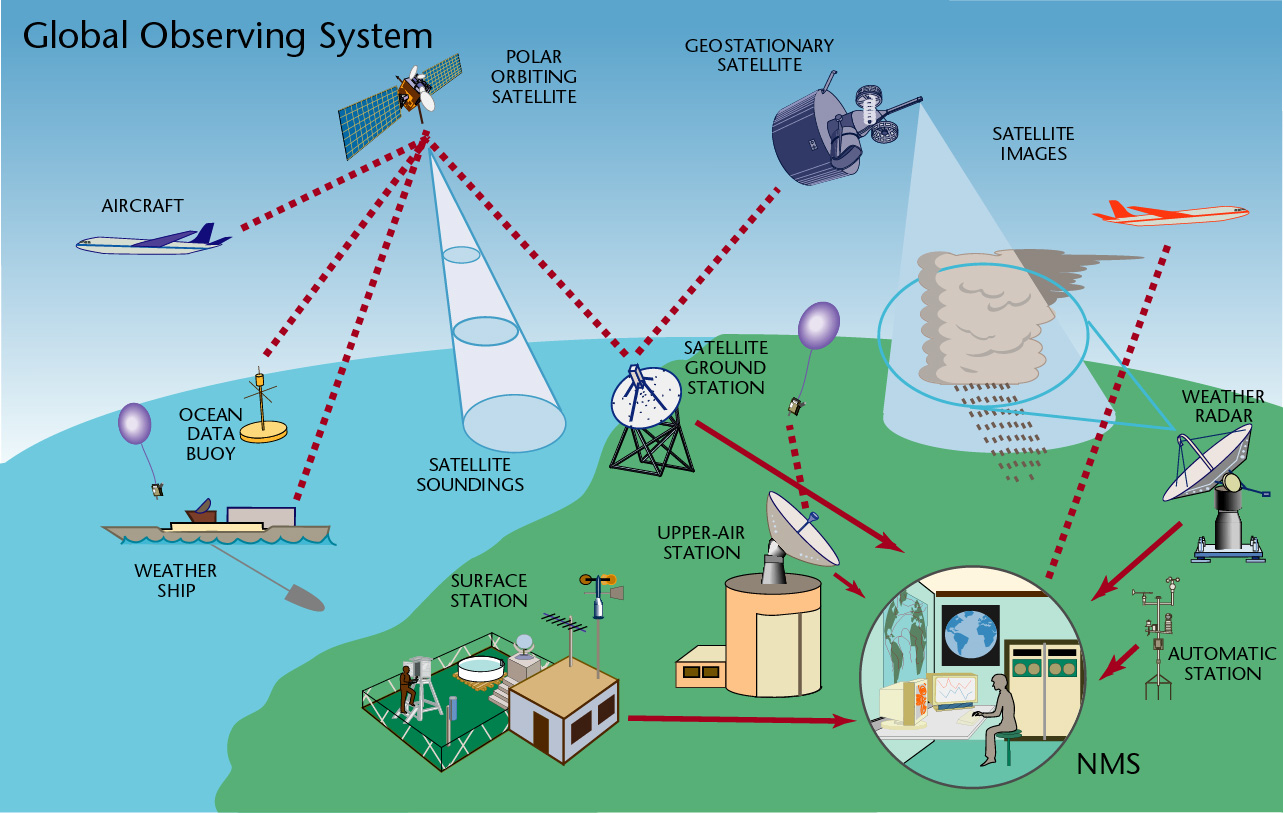
\includegraphics[width=0.66\textwidth]{./figures/gos.jpg}
    \caption{Illustration of the components of the Global Observing System (GOS) by the \textcite{worldmeteorologicalorganization2020observation}.}
    \label{fig:gos}
\end{figure}

However, better and higher-resolution instruments imply greater sensitivity to physical and chemical processes in the oceans and atmosphere, which in turn increases the complexity of the theoretical models required to interpret their measurements. The growing number of instruments also introduces new challenges in terms of quantity of collected data. Most notably, the use of satellite data has increased exponentially over the last two decades, becoming the largest contributor to forecast quality~\cite{jeppesen2020ecmwfs} and pushing current numerical weather prediction (NWP) methods to their limits. In fact, an overwhelming majority (90 to \qty{95}{\percent}) of the available satellite data is unexploited by operational NWP centers~\cite{bauer2015quiet}, including satellite channels in the visible and infrared spectrum, despite providing a wealth of information on atmospheric clouds~\cite{scheck2020assimilating, kugler2023potential}. These observations stand largely unassimilated because (a) efficient models of their measurement processes are still lacking, and (b) scaling current pipelines to ingest their volume remains computationally intractable.

Undeterred by these challenges, meteorologists across the globe continue their work towards more accurate weather prediction, for its impact is among the greatest of any field in the physical sciences~\cite{bauer2015quiet}. However, many now argue that, instead of investing solely in new instruments and increasingly sophisticated models, NWP should adopt a new computational paradigm; one that is more efficient, takes full advantage of modern hardware, and learns from the vast amounts of available data. This is where machine learning and, more specifically, deep learning come into play. Amid this abundance of data, where experts struggle to extract patterns and leverage domain knowledge, machines can learn efficient models automatically.\sidenote{\vspace{-4em}\textit{Machines take me by surprise with great frequency.}\\[1ex] --- Alan Turing (1950) \nocite{turing1950computing}} Over the past decade, this has proven true for an increasingly broad spectrum of tasks, including language modeling~\cite{vaswani2017attention, devlin2019bert, brown2020language}, voice processing~\cite{oord2016wavenet, radford2022robust, goel2022its}, image synthesis~\cite{zhu2017unpaired, karras2019stylebased, rombach2022highresolution}, autonomous agents~\cite{mnih2015humanlevel, silver2017mastering, baker2020emergent, andrychowicz2020learning, wei2022chainofthought}, and numerous scientific applications~\cite{jumper2021highly, rolnick2022tackling, degrave2022magnetic, merchant2023scaling, pfau2024accurate, manduchi2024leveraging}. Following this success, a wave of research has sought to enhance or replace NWP components with deep learning models~\cite{ravuri2021skilful, dueben2021machine, mack2020attentionbased, brajard2020combining, brajard2021combining, arcucci2021deep, fablet2021learning, frerix2021variational, buizza2022data, yeung2022physicsinformed, andrychowicz2023deep, lam2023learning}, some of which have already been integrated into operational pipelines~\cite{lang2024aifs, lentze2025ecmwfs}.

Still, unless one is akin to Laplace's demon, prediction remains fundamentally riddled with uncertainty. While there has been a long history of work to integrate deep learning models in the natural sciences, it is only recently that practitioners have started using deep \emph{probabilistic} models. These models explicitly take uncertainty into account and learn the non-deterministic relationships between the quantities of interest. Among the first deep probabilistic models were probability density estimators, including density ratio estimators \cite{tu2007learning, sugiyama2012density, gutmann2012noisecontrastive, cranmer2016approximating, cranmer2016experiments, menon2016linking, stoye2018likelihoodfree, belghazi2018mutual, durkan2020contrastive, rhodes2020telescoping, brehmer2020mining, hermans2020likelihoodfree, miller2021truncated, rozet2021arbitrary, miller2022contrastive, delaunoy2022reliable, choi2022density} and normalizing flows \cite{tabak2013family, dinh2014nice, rezende2015variational, dinh2016density, papamakarios2017masked, huang2018neural, wehenkel2019unconstrained, durkan2019neural, papamakarios2021normalizing}. One area where density estimators became the gold standard is simulation-based inference~\cite{cranmer2020frontier}, which is now recognized as a valuable extension to the statistical toolbox used in particle physics~\cite{atlascollaboration2025implementation}.

Unfortunately, density estimators have classically been restricted to low-dimensional settings, making their application to high-dimensional problems, such as those encountered in earth sciences, challenging. Furthermore, while estimating the probability density has many use cases, drawing samples from a target distribution is often the objective of probabilistic approaches. In response to these needs, a new class of deep probabilistic models has emerged, that can efficiently generate samples from high-dimensional distributions. These \emph{generative} models notably include variational auto-encoders \cite{kingma2013autoencoding, kingma2019introduction}, generative adversarial networks \cite{goodfellow2014generative}, and, most recently, diffusion models \cite{sohl-dickstein2015deep, ho2020denoising}, also known as score-based generative models \cite{song2019generative, song2021scorebased}, flow models \cite{liu2023flow, lipman2023flow}, or stochastic interpolants \cite{albergo2023stochastic}. Since their introduction, generative models have received widespread adoption in the context of image, video, and audio synthesis, and their success is now spreading to all areas of natural sciences.

\section{Research Question}

Motivated by the recent wave of research to solve scientific problems with deep probabilistic models, and the remaining obstacles to tackle high-dimensional settings, this thesis focuses on developing and applying generative models to large-scale inference problems in physics, particularly in systems whose state evolves through time, known as dynamical systems.\sidenote{\vspace{-2em}\textit{I will not define time, space, place and motion, as being well known to all.}\\[1ex] --- Isaac Newton (1687) \nocite{newton1687philosophiae}} The rapid evolution of deep learning and the modern abundance of scientific data make this objective not only timely, but a unique opportunity for technological progress.

In pursuit of this objective, this thesis explores several aspects of probabilistic modeling and dynamical systems, including state estimation, forecasting, reduced-order modeling, and learning from corrupted observations. Although motivated and developed in the context of scientific applications, the methodological contributions extend to the broader field of generative modeling.

\section{Outline}

Immediately following this introduction, we present the main contributions of this thesis, which are based on a series of peer-reviewed publications. We choose not to include an original primer on dynamical systems or deep probabilistic modeling as part of this dissertation. These topics are thoroughly covered in the literature through numerous books and reviews, and our own attempts could not match their clarity and completeness. We notably recommend two excellent reviews by \textcite{carrassi2018data} and \textcite{lai2025principles} on data assimilation and diffusion models, respectively. The background concepts and relevant literature are nevertheless discussed within the respective chapter of each contribution.

Opening the scientific part of this dissertation, Chapter \ref{chap:sda} investigates the application of diffusion models~\cite{sohl-dickstein2015deep, ho2020denoising} to the problem of state estimation in dynamical systems. This work establishes diffusion models as a promising and versatile alternative to classical data assimilation \cite{ledimet1986variational, hamill2006ensemblebased, evensen2009data, carrassi2018data, ecmwf2020ifs} methods. Chapter \ref{chap:sda-2lqg} further demonstrates that the method presented in Chapter \ref{chap:sda}, named score-based data assimilation (SDA), scales effectively to near-operational-scale systems. However, the data SDA relies on for training -- fully observed state sequences -- is rarely accessible. In practice, only incomplete and noisy observations of the states are available, especially in earth and space sciences where the systems of interest can only be probed superficially. Chapter \ref{chap:diem} addresses this limitation in the broader context of learning a prior distribution parameterized by a diffusion model when only partial and noisy observations are available. The proposed method is an adaptation of the expectation-maximization \cite{hartley1958maximum, dempster1977maximum, wu1983convergence, mclachlan2007em, balakrishnan2017statistical} algorithm tailored to diffusion models. Another limitation of SDA is its computational cost, which becomes prohibitive for long trajectories and high-dimensional states. In the context of image and video generation, this computational obstacle has been mitigated by generating in the latent space of an autoencoder rather than in pixel space. In Chapter \ref{chap:lola}, we investigate whether a similar strategy can be effectively applied to the emulation of dynamical systems, and at what cost. Our results indicate that latent modeling is a promising approach; one that is not only more efficient, but can also improve accuracy compared to physics-space models. Encouraged by these findings, we combine the latent modeling approach with the SDA framework in Chapter \ref{chap:appa}, obtaining promising results on operational-scale atmospheric data assimilation tasks.

Finally, Chapter \ref{chap:discussion} reflects upon the contributions of this thesis and discusses possible future developments in deep probabilistic modeling and its applications to dynamical systems.

\section{Publications}

The scientific content of this dissertation is exclusively borrowed from the following peer-reviewed publications, for which I played the role of lead author or project instigator.

\begin{itemize}[leftmargin=1em]
    \item[] \fullcite{rozet2023scorebased}.
    \item[] \fullcite{rozet2023scorebaseda}.
    \item[] \fullcite{rozet2024learning}.
    \item[] \fullcite{rozet2025lost}.
    \item[] \fullcite{andry2025appa}.
\end{itemize}

Throughout the pursuit of my degree, I also had the chance to take part and contribute to fruitful collaborations. The following list of publications, which are not featured in this thesis, stemmed from these collaborations.

\begin{itemize}[leftmargin=1em]
    \item[] \fullcite{hermans2022trust}.
    \item[] \fullcite{delaunoy2022reliable}.
    \item[] \fullcite{vasist2023neural}.
    \item[] \fullcite{ohana2024well}.
    \item[] \fullcite{savary2025trainingfree}.
    \item[] \fullcite{morel2025predicting}.
    \item[] \fullcite{mccabe2025walrus}.
\end{itemize}

Finally, over the past years, I have devoted a significant part of my time to free and open-source software. I consider the following Python packages, which I created and maintained during my degree, to be among its contributions.

\begin{itemize}[leftmargin=1em]
    \item[] \fullcite{rozet2021lampe}.\\ \url{https://pypi.org/project/lampe}
    \item[] \fullcite{rozet2022zuko}.\\ \url{https://pypi.org/project/zuko}
    \item[] \fullcite{rozet2024azula}.\\ \url{https://pypi.org/project/azula}
\end{itemize}

\clearpage
\section*{References}

\printbibliography[heading=none]


\newgeometry{margin=2.5cm, footskip=1cm, includefoot}
\cleardoublepage
\part{Matter} \label{part:matter}
\restoregeometry

\chapter{Score-based Data Assimilation} \label{chap:sda}

\begin{quote}
    \textit{A simple chain is an infinite sequence $x_1, x_2, \dots, x_k, x_{k+1}, \dots$ of variables connected in such a way that $x_{k+1}$ for any $k$ is independent of $x_1, x_2, \dots, x_{k-1}$ in case $x_k$ is known.}

    \begin{flushright}
        --- Andrei Markov (1906) \nocite{basharin2004life}
    \end{flushright}
\end{quote}

\vspace{2em}

\begin{addendum}{\Large\scshape Addendum}

This chapter has previously been published as

\begin{itemize}[leftmargin=1em]
    \item[] \fullcite{rozet2023scorebased}.
\end{itemize}

As the leading author, François came up with the method, formalized it, conducted the experiments, interpreted the results, and wrote the manuscript. Gilles supervised the project, suggested experiments, and participated in the writing and literature review.

For the version presented in this chapter, we have slightly edited the mathematical notations from the original publication. Notably, the diffusion time notation $x(t)$ has been replaced by the leaner $x_t$, which is more common in nowadays literature and more consistent with the rest of this document. The text itself remains unchanged, although we have enhanced it with a few retrospective comments.

\end{addendum}

\section*{Abstract}

Data assimilation, in its most comprehensive form, addresses the Bayesian inverse problem of identifying plausible state trajectories that explain noisy or incomplete observations of stochastic dynamical systems. Various approaches have been proposed to solve this problem, including particle-based and variational methods. However, most algorithms depend on the transition dynamics for inference, which becomes intractable for long time horizons or for high-dimensional systems with complex dynamics, such as oceans or atmospheres. In this work, we introduce score-based data assimilation for trajectory inference. We learn a score-based generative model of state trajectories based on the key insight that the score of an arbitrarily long trajectory can be decomposed into a series of scores over short segments. After training, inference is carried out using the score model, in a non-autoregressive manner by generating all states simultaneously. Quite distinctively, we decouple the observation model from the training procedure and use it only at inference to guide the generative process, which enables a wide range of zero-shot observation scenarios. We present theoretical and empirical evidence supporting the effectiveness of our method.

\section{Introduction}

Data assimilation (DA) \cite{lorenc1986analysis, ledimet1986variational, evensen1994sequential, hamill2006ensemblebased,tremolet2006accounting, tremolet2007modelerror, fisher2011weakconstraint, carrassi2018data, ecmwf2020ifs} is at the core of many scientific domains concerned with the study of complex dynamical systems such as atmospheres, oceans or climates. The purpose of DA is to infer the state of a system evolving over time based on various sources of imperfect information, including sparse, intermittent, and noisy observations.

Formally, let $x^{1:L} = (x^1, x^2, \dots, x^L) \in \mathbb{R}^{L \times D}$ denote a trajectory of states in a discrete-time stochastic dynamical system and $p(x^{i+1} \mid x^i)$ be the transition dynamics from state $x^i$ to state $x^{i+1}$. An observation $y \in \mathbb{R}^M$ of the state trajectory $x^{1:L}$ follows an observation process $p(y \mid x^{1:L})$, generally formulated as $y = \mathcal{A}(x^{1:L}) + \eta$, where the measurement function $\mathcal{A}: \mathbb{R}^{L \times D} \mapsto \mathbb{R}^M$ is often non-linear and the observational error $\eta \in \mathbb{R}^M$ is a stochastic additive term that accounts for instrumental noise and systematic uncertainties. In this framework, the goal of DA is to solve the inverse problem of inferring plausible trajectories $x^{1:L}$ given an observation $y$, that is, to estimate the trajectory posterior
\begin{equation}
    p(x^{1:L} \mid y) = \frac{p(y \mid x^{1:L})}{p(y)} \, p(x^1) \prod_{i=1}^{L-1} p(x^{i+1} \mid x^i)
\end{equation}
where the initial state prior $p(x^1)$ is commonly referred to as background \cite{tremolet2006accounting, tremolet2007modelerror, fisher2011weakconstraint, carrassi2018data, ecmwf2020ifs}. In geosciences, the amount of data available is generally insufficient to recover the full state of the system from the observation alone \cite{carrassi2018data}. For this reason, the physical model underlying the transition dynamics is of paramount importance to fill in spatial and temporal gaps in the observation.

State-of-the-art approaches to data assimilation are based on variational assimilation \cite{lorenc1986analysis, ledimet1986variational, tremolet2006accounting, tremolet2007modelerror, fisher2011weakconstraint}. Many of these approaches formulate the task as a maximum-a-posteriori (MAP) estimation problem and solve it by maximizing the log-posterior density $\log p(x^{1:L} \mid y)$ via gradient ascent. Although this approach only produces a point estimate of the trajectory posterior, its cost can already be substantial for problems of the size and complexity of geophysical systems, since it requires differentiating through the physical model. The amount of data that can be assimilated is therefore restricted because of computational limitations. For example, only a small volume of the available satellite data is exploited for operational forecasts and yet, even with these restrictions, data assimilation accounts for a significant fraction of the computational cost for modern numerical weather prediction \cite{bauer2015quiet, gustafsson2018survey}.
%
Recent work has shown that deep learning can be used in a variety of ways to improve the computational efficiency of data assimilation, increase the reconstruction performance by estimating unresolved scales after data assimilation, or integrate multiple sources of observations \cite{mack2020attentionbased, arcucci2021deep, frerix2021variational, fablet2021learning,yeung2022physicsinformed, brajard2020combining, brajard2021combining, zhang2022multisource}.

\paragraph{Contributions}
In this work, we propose a novel approach to data assimilation based on score-based generative models. Leveraging the Markovian structure of dynamical systems, we train a score network from short segments of trajectories which is then capable of generating physically consistent and arbitrarily-long state trajectories. The observation model is decoupled from the score network and used only during assimilation to guide the generative process, which allows for a wide range of zero-shot observation scenarios. Our approach provides an accurate approximation of the whole trajectory posterior -- it is not limited to point estimates -- without simulating or differentiating through the physical model. The code for all experiments is made available at \url{https://github.com/francois-rozet/sda}.

\section{Background}

Score-based generative models have recently shown remarkable capabilities, powering many of the latest advances in image, video or audio generation \cite{rombach2022highresolution, ramesh2022hierarchical, saharia2022photorealistic, ho2022video, ho2022cascaded, ho2022imagen, kong2021diffwave, goel2022its}. In this section, we review score-based generative models and outline how they can be used for solving inverse problems.

\paragraph{Continuous-time score-based generative models}
Adapting the formulation of \textcite{song2021scorebased}, samples $x \in \mathbb{R}^D$ from a distribution $p(x)$ are progressively perturbed through a continuous-time diffusion process expressed as a linear stochastic differential equation (SDE)
\begin{equation} \label{eq:sda-forward-sde}
    \d{x_t} = f_t \, x_t \d{t} + g_t \d{w_t}
\end{equation}
where $f_t \in \mathbb{R}$ is the drift coefficient, $g_t \in \mathbb{R}$ is the diffusion coefficient, $w_t \in \mathbb{R}^D$ denotes a Wiener process (standard Brownian motion) and $x_t \in \mathbb{R}^D$ is the perturbed sample at time $t \in [0, 1]$. Because the SDE is linear with respect to $x_t$, the perturbation kernel from $x$ to $x_t$ is Gaussian and takes the form
\begin{equation}
    p(x_t \mid x) = \mathcal{N}(x_t \mid \alpha_t \, x, \Sigma_t)
\end{equation}
where $\alpha_t$ and $\Sigma_t = \sigma_t^2 I$ can be derived analytically from $f_t$ and $g_t$ \cite{sarkka2019applied, zhang2023fast}. Denoting $p(x_t)$ the marginal distribution of $x_t$, we impose that $\alpha_0 = 1$ and $\sigma_0 \ll 1$, such that $p(x_0) \approx p(x)$, and we chose the coefficients $f_t$ and $g_t$ such that the influence of the initial sample $x$ on the final perturbed sample $x_1$ is negligible with respect to the noise level -- that is, $p(x_1) \approx \mathcal{N}(0, \Sigma_1)$. The variance exploding (VE) and variance preserving (VP) SDEs \cite{song2019generative, ho2020denoising, song2021scorebased} are widespread examples satisfying these constraints.

Crucially, the time reversal of the forward SDE \eqref{eq:sda-forward-sde} is given by a reverse SDE \cite{anderson1982reversetime, song2021scorebased}
\begin{equation} \label{eq:sda-reverse-sde}
    \d{x_t} = \left[ f_t \, x_t - g_t^2 \, \grad{x_t} \log p(x_t) \right] \d{t} + g_t \d{w_t} .
\end{equation}
That is, we can draw noise samples $x_1 \sim \mathcal{N}(0, \Sigma_1)$ and gradually remove the noise therein to obtain data samples $x_0 \sim p(x_0)$ by simulating the reverse SDE from $t = 1$ to $0$. This requires access to the quantity $\grad{x_t} \log p(x_t)$ known as the score of $p(x_t)$.

\paragraph{Denoising score matching}
In practice, the score $\grad{x_t} \log p(x_t)$ is approximated by a neural network $s_\phi(x_t, t)$, named the score network, which is trained to solve the denoising score matching objective \cite{hyvarinen2005estimation, vincent2011connection, song2021scorebased}
\begin{equation} \label{eq:sda-dsm-objective}
    \arg\min_\phi \mathbb{E}_{p(x) p_t p(x_t \mid x)} \left[ \sigma_t^2 \left\| s_\phi(x_t, t) - \grad{x_t} \log p(x_t \mid x) \right\|_2^2 \right]
\end{equation}
where $p_t = \mathcal{U}(0, 1)$. The theory of denoising score matching ensures that $s_\phi(x_t, t) \approx \grad{x_t} \log p(x_t)$ for a sufficiently expressive score network. After training, the score network is plugged into the reverse SDE \eqref{eq:sda-reverse-sde}, which is then simulated using an appropriate discretization scheme \cite{song2021scorebased, song2021denoising, liu2022pseudo, zhang2023fast}.

\sidenote{\vspace{1cm} \itshape We later found out that the EDM \cite{karras2022elucidating} or flow \cite{liu2023flow} parameterizations would have been better choices.}
In practice, the high variance of $\grad{x_t} \log p(x_t \mid x)$ near $t = 0$ makes the optimization of \eqref{eq:sda-dsm-objective} unstable \cite{zhang2023fast}. To mitigate this issue, a slightly different parameterization $\epsilon_\phi(x_t, t) = -\sigma_t \, s_\phi(x_t, t)$ of the score network is often used, which leads to the otherwise equivalent objective \cite{ho2020denoising, song2021denoising, zhang2023fast}
\begin{equation} \label{eq:sda-ddpm-objective}
    \arg\min_\phi \mathbb{E}_{p(x) p_t p(\epsilon)} \left[ \left\| \epsilon_\phi(\alpha_t \, x + \sigma_t \, \epsilon, t) - \epsilon\right\|_2^2 \right]
\end{equation}
where $p(\epsilon) = \mathcal{N}(0, I)$. In the following, we keep the score network notation $s_\phi(x_t, t)$ for convenience, even though we adopt the parameterization $\epsilon_\phi(x_t, t)$ and its objective for our experiments.

\paragraph{Zero-shot inverse problems}
With score-based generative models, we can generate samples from the unconditional distribution $p(x_0) \approx p(x)$. To solve inverse problems, however, we need to sample from the posterior distribution $p(x \mid y)$. This could be accomplished by training a conditional score network $s_\phi(x_t, t \mid y)$ to approximate the posterior score $\grad{x_t} \log p(x_t \mid y)$ and plugging it into the reverse SDE \eqref{eq:sda-reverse-sde}. However, this would require data pairs $(x, y)$ during training and one would need to retrain a new score network each time the observation process $p(y \mid x)$ changes. Instead, many have observed \cite{song2021scorebased, kawar2021snips, song2022solving, adam2022posterior, chung2023diffusion} that the posterior score can be decomposed into two terms thanks to Bayes' rule
\begin{equation} \label{eq:sda-score-bayes}
    \grad{x_t} \log p(x_t \mid y) = \grad{x_t} \log p(x_t) + \grad{x_t} \log p(y \mid x_t) .
\end{equation}
Since the prior score $\grad{x_t} \log p(x_t)$ can be approximated with a single score network, the remaining task is to estimate the likelihood score $\grad{x_t} \log p(y \mid x_t)$. Assuming a differentiable measurement function $\mathcal{A}$ and a Gaussian observation process $p(y \mid x) = \mathcal{N}(y \mid \mathcal{A}(x), \Sigma_y)$, \textcite{chung2023diffusion} propose the approximation
\begin{equation} \label{eq:sda-likelihood-approx-dps}
    p(y \mid x_t) = \int p(y \mid x) \, p(x \mid x_t) \d{x} \approx \mathcal{N} \left(y \mid \mathcal{A}(\hat{x}(x_t)), \Sigma_y \right)
\end{equation}
where the mean $\hat{x}(x_t) = \mathbb{E}_{p(x \mid x_t)} [x]$ is given by Tweedie's formula \cite{efron2011tweedies, kim2021noise2score}
\begin{align}
    \mathbb{E}_{p(x \mid x_t)} [x] & = \frac{x_t + \sigma_t^2 \, \grad{x_t} \log p(x_t)}{\alpha_t} \label{eq:sda-tweedie} \\
    & \approx \frac{x_t + \sigma_t^2 \, s_\phi(x_t, t)}{\alpha_t} \, .
\end{align}
As the log-likelihood of a multivariate Gaussian is known analytically and $s_\phi(x_t, t)$ is differentiable, we can compute the likelihood score $\grad{x_t} \log p(y \mid x_t)$ with this approximation in zero-shot, that is, without training any other network than $s_\phi(x_t, t)$.

\section{Score-based data assimilation}

Coming back to our initial inference problem, we want to approximate the trajectory posterior $p(x^{1:L} \mid y)$ of a dynamical system. To do so with score-based generative modeling, we need to estimate the posterior score $\grad{x^{1:L}_t} \log p(x^{1:L}_t \mid y)$, which we choose to decompose into prior and likelihood terms, as in \eqref{eq:sda-score-bayes}, to enable a wide range of zero-shot observation scenarios.

In typical data assimilation settings, the high-dimensionality of each state $x^i$ (e.g. the state of atmospheres or oceans) combined with potentially long trajectories would require an impractically large score network $s_\phi(x^{1:L}_t, t)$ to estimate the prior score $\grad{x^{1:L}_t} \log p(x^{1:L}_t)$ and a proportional amount of data for training, which could be prohibitive if data is scarce or if the physical model is expensive to simulate. To overcome this challenge, we leverage the Markovian structure of dynamical systems to approximate the prior score with a series of local scores, which are easier to learn, as explained in Section \ref{sec:sda-sda-blanket}.
%
In Section \ref{sec:sda-sda-likelihood-score}, we build upon diffusion posterior sampling (DPS) \cite{chung2023diffusion} to propose a new approximation for the likelihood score $\grad{x^{1:L}_t} \log p(y \mid x^{1:L}_t)$, which we find more appropriate for posterior inference. Finally, in Section \ref{sec:sda-sda-pc-sampling}, we describe our sampling procedure inspired from predictor-corrector sampling \cite{song2021scorebased}. Our main contribution, named score-based data assimilation (SDA), is the combination of these three components.

\subsection{How is your blanket?} \label{sec:sda-sda-blanket}
\sidenote{\vspace{-1.75cm} \itshape This section's title is a reference to OSS 117, a classic french comedy movie. To our delight, one of the reviewers noticed this reference, and replied with another reference:\\ \enquote{The blanket is good.}}

Given a set of random variables $x^{1:L} = \{ x^1, x^2, \dots, x^L \}$, it is sometimes possible to find a small Markov blanket $x^{b_i} \subseteq x^{\neq i}$ such that $p(x^i \mid x^{\neq i}) = p(x^i \mid x^{b_i})$ for each element $x^i$ using our knowledge of the set's structure. It follows that each element $\grad{x^i} \log p(x^{1:L})$ of the full score $\grad{x^{1:L}} \log p(x^{1:L})$ can be determined locally, that is, only using its blanket;
\begin{align}
    \grad{x^i} \log p(x^{1:L}) & = \grad{x^i} \log p(x^i \mid x^{\neq i}) + \grad{x^i} \log p(x^{\neq i}) \\
    & = \grad{x^i} \log p(x^i \mid x^{b_i}) + \grad{x^i} \log p(x^{b_i}) = \grad{x^i} \log p(x^i, x^{b_i}).
\end{align}
This property generally does not hold for the diffusion-perturbed set $x^{1:L}_t$ as there is no guarantee that $x^{b_i}_t$ is a Markov blanket of the element $x^i_t$. However, there exists a set of indices $\bar{b}_i \supseteq b_i$ such that
\begin{equation} \label{eq:sda-pseudo-blanket}
   \grad{x^i_t} \log p(x^{1:L}_t) \approx \grad{x^i_t} \log p(x^i_t, x^{\bar{b}_i}_t)
\end{equation}
is a good approximation for all $t \in [0, 1]$. That is, $x^{\bar{b}_i}_t$ is a \enquote{pseudo} Markov blanket of $x^i_t$. In the worst case, $\bar{b}_i$ contains all indices except $i$, but we argue that, for some structures, there is a set $\bar{b}_i$ not much larger than $b_i$ that satisfies \eqref{eq:sda-pseudo-blanket}. Our rationale is that, since we impose the initial noise to be negligible, we know that $x^{b_i}_t$ becomes indistinguishable from $x^{b_i}$ as $t$ approaches $0$. Furthermore, as $t$ grows and noise accumulates, the mutual information between elements $x^i_t$ and $x^j_t$ decreases to finally reach $0$ when $t = 1$. Hence, even if $\bar{b}_i = b_i$, the pseudo-blanket approximation \eqref{eq:sda-pseudo-blanket} already holds near $t = 0$ and $t = 1$. In between, even though the approximation remains unbiased (see Appendix \ref{app:sda-unbiased}), the structure of the set becomes decisive. If it is known and present enough regularities/symmetries, \eqref{eq:sda-pseudo-blanket} could and should be exploited within the architecture of the score network $s_\phi(x^{1:L}_t, t)$.

\begin{figure}[t]
    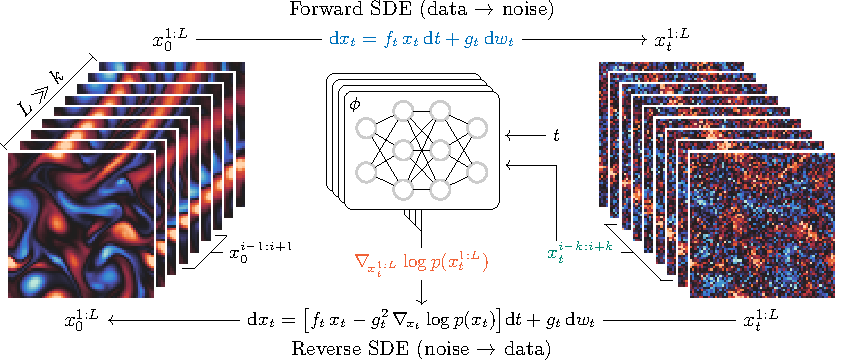
\includegraphics[width=\textwidth]{./chapters/sda/figures/diffusion.pdf}
    \caption{Trajectories $x^{1:L}$ of a dynamical system are transformed to noise via a \textcolor{RoyalBlue}{diffusion process}. Reversing this process generates new trajectories, but requires the \textcolor{RedOrange}{score of $p(x^{1:L}_t)$}. We approximate it by combining the outputs of a score network over \textcolor{PineGreen}{sub-segments of $x^{1:L}_t$}.}
    \label{fig:diffusion}
\end{figure}
\sidenote{\vspace{-14.5cm} \itshape The lines connecting the stack of networks and the score $\grad{x_t^{1:L}} \log p(x_t^{1:L})$ represent Algorithm \ref{alg:composing}.}

\sidenote{\vspace{2cm} \itshape In hindsight, systems governed by slowly evolving dynamics require much wider windows\\ than we expected.}
In the case of dynamical systems, the set $x^{1:L}$ is by definition a first-order Markov chain and the minimal Markov blanket of an element $x^i$ is $x^{b_i} = \{x^{i-1}, x^{i+1}\}$. For the perturbed element $x^i_t$, the pseudo-blanket $x^{\bar{b}_i}_t$ can take the form of a window surrounding $x^i_t$, that is $\bar{b}_i = \{i-k, \dots, i+k\} \setminus \{i\}$ with $k \geq 1$. The value of $k$ is dependent on the problem, but we argue, supported by our experiments, that it is generally much smaller than the chain's length $L$. Hence, a fully convolutional neural network (FCNN) with a narrow receptive field is well suited to the task, and long-range capabilities would be wasted resources. Importantly, if the receptive field is $2k + 1$, the network can be trained on segments $x^{i-k:i+k}$ instead of the full chain $x^{1:L}$, thereby drastically reducing training costs. More generally, we can train a local score network (see Algorithm \ref{alg:training})
\begin{equation}
    s_\phi(x^{i-k:i+k}_t, t) \approx \grad{x^{i-k:i+k}_t} \log p(x^{i-k:i+k}_t)
\end{equation}
such that its $k+1$-th element approximates the score of the $i$-th state $\grad{x^i_t} \log p(x^{1:L}_t)$. We also have that the $k$ first elements of $s_\phi(x^{1:2k+1}_t, t)$ approximate the score of the $k$ first states $\grad{x^{1:k}_t} \log p(x^{1:L}_t)$ and the $k$ last elements of $s_\phi(x^{L-2k:L}_t, t)$ approximate the score of the $k$ last states $\grad{x^{L-k:L}_t} \log p(x^{1:L}_t)$. Hence, we can apply the local score network on all sub-segments $x^{i-k:i+k}_t$ of $x^{1:L}_t$, similar to a convolution kernel, and combine the outputs (see Algorithm \ref{alg:composing}) to get an approximation of the full score $\grad{x^{1:L}_t} \log p(x^{1:L}_t)$. Note that we can either condition the score network with $i$ or assume the statistical stationarity of the chain, that is $p(x^i) = p(x^{i+1})$.

\begin{figure}[t]
\begin{minipage}[t]{0.49\textwidth}%
\vspace{-1em}
\begin{algorithm}[H]
    \caption{Training $\epsilon_\phi(x^{i-k:i+k}_t, t)$} \label{alg:training}
    \begin{algorithmic}[1]
        \For{$i = 1$ to $N$}
            \State $x^{1:L} \sim p(x^{1:L})$
            \State $i \sim \mathcal{U}(\{k+1, \dots, L-k\})$
            \State $t \sim \mathcal{U}(0, 1), \epsilon \sim \mathcal{N}(0, I)$
            \State $x^{i-k:i+k}_t \gets \alpha_t \, x^{i-k:i+k} + \sigma_t \, \epsilon$
            \State $\displaystyle \ell \gets \| \epsilon_\phi(x^{i-k:i+k}_t, t) - \epsilon \|_2^2$
            \State $\phi \gets \Call{GradientDescent}{\phi, \grad{\phi} \, \ell}$
        \EndFor{}
	\end{algorithmic}
\end{algorithm}
\end{minipage}
\hfill
\begin{minipage}[t]{0.49\textwidth}%
\vspace{-1em}
\begin{algorithm}[H]
    \caption{Composing $s_\phi(x^{i-k:i+k}_t, t)$} \label{alg:composing}
    \begin{algorithmic}[1]
        \Function{$s_\phi(x^{1:L}_t, t)$}{}
            \State $s_{1:k+1} \gets s_\phi(x^{1:2k+1}_t, t)[:\!k + 1]$
            \For{$i = k + 2$ to $L - k - 1$}
                \State $s_i \gets s_\phi(x^{i-k:i+k}_t, t)[k+1]$
            \EndFor{}
            \State $s_{L-k:L} \gets s_\phi(x^{L-2k:L}_t, t)[k+1\!:]$
            \State \Return{$s^{1:L}$}
        \EndFunction{}
	\end{algorithmic}
\end{algorithm}
\end{minipage}
\end{figure}

\subsection{Stable likelihood score} \label{sec:sda-sda-likelihood-score}

Due to approximation and numerical errors in $\hat{x}(x_t)$, computing the score $\grad{x_t} \log p(y \mid x_t)$ with the likelihood approximation \eqref{eq:sda-likelihood-approx-dps} is very unstable, especially in the low signal-to-noise regime, that is when $\sigma_t \gg \alpha_t$. This incites \textcite{chung2023diffusion} to replace the covariance $\Sigma_y$ by the identity $I$ and rescale the likelihood score with respect to $\|y - \mathcal{A}(\hat{x}(x_t))\|$ to stabilize the sampling process. These modifications introduce a significant error in the approximation as they greatly affect the norm of the likelihood score.

\sidenote{\vspace{2.5cm} \itshape This was the start of our journey towards better likelihood score approximations, which eventually led to the development of MMPS \cite{rozet2024learning}.}
We argue that the instability is due to \eqref{eq:sda-likelihood-approx-dps} being only exact if the variance of $p(x \mid x_t)$ is null or negligible, which is not the case when $t > 0$. Instead, \textcite{adam2022posterior} and \textcite{meng2022diffusion} approximate the covariance of $p(x \mid x_t)$ with $\nicefrac{\Sigma_t}{\alpha_t^2}$, which is valid as long as the prior $p(x)$ is Gaussian with a large diagonal covariance $\Sigma_x$. We motivate in Appendix \ref{app:sda-covariance} the more general covariance approximation $\nicefrac{\sigma_t^2}{\alpha_t^2} \Gamma$, where the matrix $\Gamma$ depends on the eigendecomposition of $\Sigma_x$. Then, taking inspiration from the extended Kalman filter, we approximate the perturbed likelihood as
\begin{equation} \label{eq:sda-likelihood-approx}
    p(y \mid x_t) \approx \mathcal{N} \left( y \mid \mathcal{A}(\hat{x}(x_t)), \Sigma_y + \frac{\sigma_t^2}{\alpha_t^2} A \Gamma A^T \right)
\end{equation}
where $A = \partial_x \, \mathcal{A} \mid_{\hat{x}(x_t)}$ is the Jacobian of $\mathcal{A}$. In practice, to simplify the approximation, the term $A \Gamma A^T$ can often be replaced by a constant (diagonal) matrix. We find that computing the likelihood score $\grad{x_t} \log p(y \mid x_t)$ with this new approximation (see Algorithm \ref{alg:posterior}) is stable enough that rescaling it or ignoring $\Sigma_y$ is unnecessary.

\subsection{Predictor-Corrector sampling}
\label{sec:sda-sda-pc-sampling}

To simulate the reverse SDE, we adopt the exponential integrator (EI) discretization scheme introduced by \textcite{zhang2023fast}
\begin{equation} \label{eq:sda-predictor}
    x_{t - \Delta t} \gets \frac{\alpha_{t - \Delta t}}{\alpha_t} x_t + \left( \frac{\alpha_{t - \Delta t}}{\alpha_t} - \frac{\sigma_{t - \Delta t}}{\sigma_t} \right) \sigma_t^2 \, s_\phi(x_t, t)
\end{equation}
which coincides with the deterministic DDIM \cite{song2021denoising} sampling algorithm when the variance preserving SDE \cite{ho2020denoising} is used. However, as we approximate both the prior and likelihood scores, errors accumulate along the simulation and cause it to diverge, leading to low-quality samples. To prevent errors from accumulating, we perform (see Algorithm \ref{alg:sampling}) a few steps of Langevin Monte Carlo (LMC) \cite{parisi1981correlation, grenander1994representations}
\begin{equation} \label{eq:sda-corrector}
    x_t \gets x_t + \delta \, s_\phi(x_t, t) + \sqrt{2 \delta} \, \epsilon
\end{equation}
where $\epsilon \sim \mathcal{N}(0, I)$, between each step of the discretized reverse SDE \eqref{eq:sda-predictor}. In the limit of an infinite number of LMC steps with a sufficiently small step size $\delta \in \mathbb{R}_+$, simulated samples are guaranteed to follow the distribution implicitly defined by our approximation of the posterior score at each time $t$, meaning that the errors introduced by the pseudo-blanket \eqref{eq:sda-pseudo-blanket} and likelihood \eqref{eq:sda-likelihood-approx} approximations do not accumulate. In practice, we find that few LMC steps are necessary. \textcite{song2021scorebased} introduced a similar strategy, named predictor-corrector (PC) sampling, to correct the errors introduced by the discretization of the reverse SDE.

\section{Results}

We demonstrate the effectiveness of score-based data assimilation on two chaotic dynamical systems: the Lorenz 1963 \cite{lorenz1963deterministic} and Kolmogorov flow \cite{chandler2013invariant} systems. The former is a simplified mathematical model for atmospheric convection. Its low dimensionality enables posterior inference using classical sequential Monte Carlo methods \cite{liu1998sequential, doucet2011tutorial} such as the bootstrap particle filter \cite{gordon1993novel}. This allows us to compare objectively our posterior approximations against the ground-truth posterior. The second system considers the state of a two-dimensional turbulent fluid subject to Kolmogorov forcing \cite{chandler2013invariant}. The evolution of the fluid is modeled by the Navier-Stokes equations, the same equations that underlie the models of oceans and atmospheres. This task provides a good understanding of how SDA would perform in typical data assimilation applications, although our analysis is primarily qualitative due to the unavailability of reliable assessment tools for systems of this scale.

For both systems, we employ as diffusion process the variance preserving SDE with a cosine schedule \cite{nichol2021improved}, that is $\alpha_t = \cos(\omega t)^2$ with $\omega = \arccos \sqrt{10^{-3}}$ and $\sigma_t = \sqrt{1 - \alpha_t^2}$. The score networks are trained once and then evaluated under various observation scenarios. Unless specified otherwise, we estimate the posterior score according to Algorithm \ref{alg:posterior} with $\Gamma = \num{e-2} I$ and simulate the reverse SDE \eqref{eq:sda-reverse-sde} according to Algorithm \ref{alg:sampling} in \num{256} evenly spaced discretization steps.

\subsection{Lorenz 1963}

The state $x = (a, b, c) \in \mathbb{R}^3$ of the Lorenz system evolves according to a system of ordinary differential equations
\begin{equation} \label{eq:sda-lorenz}
\begin{aligned}
    \dot{a} & = \sigma (b - a) \\
    \dot{b} & = a (\rho - c) - b \\
    \dot{c} & = ab - \beta c
\end{aligned}
\end{equation}
where $\sigma = 10$, $\rho = 28$ and $\beta = \frac{8}{3}$ are parameters for which the system exhibits a chaotic behavior. We denote $\tilde{a}$ and $\tilde{c}$ the standardized (zero mean and unit variance) versions of $a$ and $c$, respectively. As our approach assumes a discrete-time stochastic dynamical system, we consider a transition process of the form $x^{i+1} = \mathcal{M}(x^i) + \eta$, where $\mathcal{M}: \mathbb{R}^3 \mapsto \mathbb{R}^3$ is the integration of the differential equations \eqref{eq:sda-lorenz} for $\Delta = \num{0.025}$ time units and $\eta \sim \mathcal{N}(0, \Delta I)$ represents Brownian noise.

\begin{figure}[!t]
    \centering
    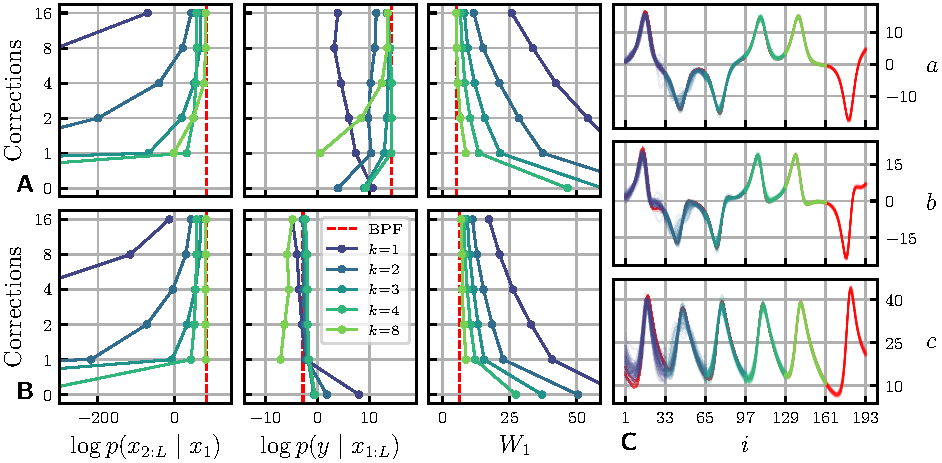
\includegraphics[scale=0.75]{./chapters/sda/figures/statistics.pdf}
    \caption{Average posterior summary statistics over 64 observations from the low (\textbf{\textsf{A}}) and high (\textbf{\textsf{B}}) frequency observation processes. We observe that, as $k$ and the number of corrections $C$ increase, the statistics of the approximate posteriors get closer to the ground-truth, in red, which means they are getting more accurate. However, increasing $k$ and $C$ improves the quality of posteriors with decreasing return, such that all posteriors with $k \geq 3$ and $C \geq 2$ are almost equivalent. This is visible in \textbf{\textsf{C}}, where we display trajectories inferred ($C=2$) for an observation of the low frequency observation process. For readability, we allocate a segment of 32 states to each $k$ instead of overlapping all 192 states. Note that the Wasserstein distance between the ground-truth posterior and itself is not zero as it is estimated with a finite number (1024) of samples.}
    \vspace{-0.5em}
    \label{fig:statistics}
\end{figure}

We generate \num{1024} independent trajectories of \num{1024} states, which are split into training (\qty{80}{\percent}), validation (\qty{10}{\percent}) and evaluation (\qty{10}{\percent}) sets. The initial states are drawn from the statistically stationary regime of the system. We consider two score network architectures: fully-connected local score networks for small $k$ ($k \leq 4$) and fully-convolutional score networks for large $k$. Architecture and training details for each $k$ are provided in Appendix \ref{app:sda-details}.

We first study the impact of $k$ (see Section \ref{sec:sda-sda-blanket}) and the number of LMC corrections (see Section \ref{sec:sda-sda-pc-sampling}) on the quality of the inferred posterior. We consider two simple observation processes $\mathcal{N}(y \mid \tilde{a}^{1:L:8}, 0.05^2 I)$ and $\mathcal{N}(y \mid \tilde{a}^{1:L}, 0.25^2 I)$. The former observes the state at low frequency (every eighth step) with low noise, while the latter observes the state at high frequency (every step) with high noise. For both processes, we generate an observation $y$ for a trajectory of the evaluation set (truncated at $L=65$) and apply the bootstrap particle filter (BPF) to draw \num{1024} trajectories $x^{1:L}$ from the ground-truth posterior $p(x^{1:L} \mid y)$. We use a large number of particles ($2^{16}$) to ensure convergence. Then, using SDA, we sample $1024$ trajectories from the approximate posterior $q(x^{1:L} \mid y)$ defined by each score network. We compare the approximate and ground-truth posteriors with three summary statistics: the expected log-prior $\mathbb{E}_{q(x^{1:L} \mid y)} [\log p(x^{2:L} \mid x^1)]$, the expected log-likelihood $\mathbb{E}_{q(x^{1:L} \mid y)} [\log p(y\mid x^{1:L})]$ and the Wasserstein distance $W_1(p, q)$ in trajectory space. We repeat the procedure for \num{64} observations and different number of corrections ($\tau = 0.25$, see Algorithm \ref{alg:sampling}) and present the results in Figure \ref{fig:statistics}. To paraphrase, SDA is able to reproduce the ground-truth posterior accurately. Interestingly, accuracy can be traded off for computational efficiency: fewer corrections leads to faster inference at the potential expense of physical consistency.

Another advantage of SDA over variational data assimilation approaches is that it targets the whole posterior distribution instead of point estimates, which allows to identify when several scenarios are plausible. As a demonstration, we generate an observation from the observation process $p(y \mid x^{1:L}) = \mathcal{N}(y \mid \tilde{c}^{1:L:4}, 0.1^2 I)$ and infer plausible trajectories with SDA ($k=4$, $C=2$). Several modes are identified in the posterior, which we illustrate in Figure \ref{fig:multimodal}.

\begin{figure}[!t]
    \centering
    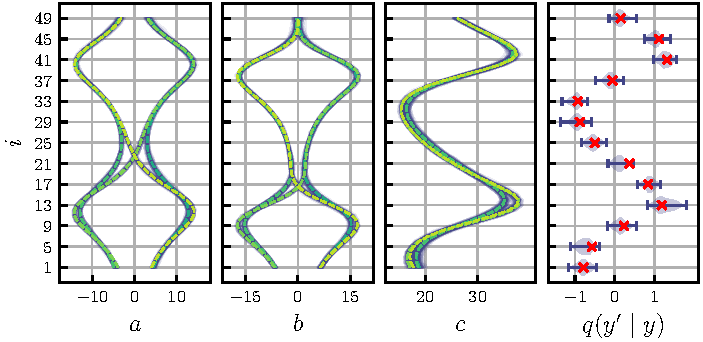
\includegraphics[scale=0.75]{./chapters/sda/figures/multimodal.pdf}
    \caption{Example of multi-modal posterior inference with SDA. We identify four modes (dashed lines) in the inferred posterior. All modes are consistent with the observation (red crosses), as demonstrated by the posterior predictive distribution $q(y' \mid y) = \mathbb{E}_{q(x^{1:L} \mid y)} [ p(y' \mid x^{1:L}) ]$.}
    \label{fig:multimodal}
\end{figure}

\subsection{Kolmogorov flow}

\begin{figure}[!b]
    \centering
    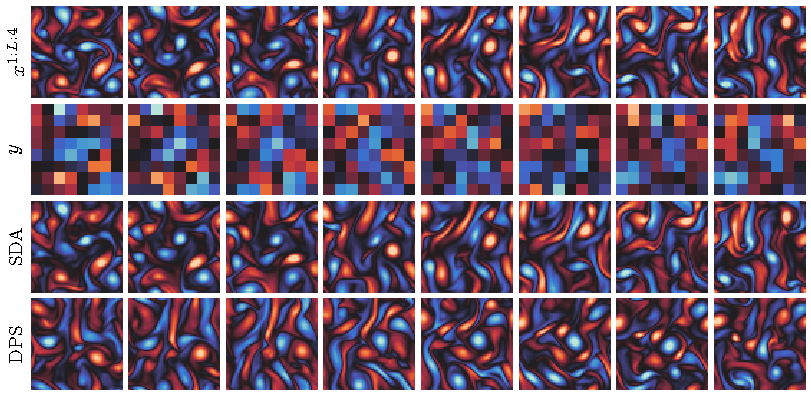
\includegraphics[scale=0.85]{./chapters/sda/figures/assimilation.pdf}
    \caption{Example of sampled trajectory from coarse, intermittent and noisy observations. States are visualized by their vorticity field $\omega = \nabla \times \bm{u}$, that is the curl of the velocity field. Positive values (red) indicate clockwise rotation and negative values (blue) indicate counter-clockwise rotation. SDA closely recovers the original trajectory, despite the limited amount of available data. Replacing SDA's likelihood score approximation with the one of DPS \cite{chung2023diffusion} yields trajectories inconsistent with the observation.}
    \label{fig:assimilation}
\end{figure}

Incompressible fluid dynamics are governed by the Navier-Stokes equations
\begin{equation} \label{eq:sda-navier-stokes}
\begin{aligned}
    \dot{\bm{u}} & = - \bm{u} \nabla \bm{u} + \frac{1}{Re} \nabla^2 \bm{u} - \frac{1}{\rho} \nabla p + \bm{f} \\
    0 & = \nabla \cdot \bm{u}
\end{aligned}
\end{equation}
where $\bm{u}$ is the velocity field, $Re$ is the Reynolds number, $\rho$ is the fluid density, $p$ is the pressure field and $\bm{f}$ is the external forcing. Following \textcite{kochkov2021machine}, we choose a two-dimensional domain $[0, 2 \pi]^2$ with periodic boundary conditions, a large Reynolds number $Re = \num{e3}$, a constant density $\rho = 1$ and an external forcing $\bm{f}$ corresponding to Kolmogorov forcing with linear damping \cite{chandler2013invariant, boffetta2012twodimensional}. We use the \href{https://github.com/google/jax-cfd}{\texttt{jax-cfd}} library \cite{kochkov2021machine} to solve the Navier-Stokes equations \eqref{eq:sda-navier-stokes} on a $256 \times 256$ domain grid. The states $x^i$ are snapshots of the velocity field $\bm{u}$, coarsened to a $64 \times 64$ resolution, and the integration time between two such snapshots is $\Delta = 0.2$ time units. This corresponds to \num{82} integration steps of the forward Euler method, which would be expensive to differentiate through repeatedly, as required by gradient-based data assimilation approaches.

We generate \num{1024} independent trajectories of \num{64} states, which are split into training (\qty{80}{\percent}), validation (\qty{10}{\percent}) and evaluation (\qty{10}{\percent}) sets. The initial states are drawn from the statistically stationary regime of the system. We consider a local score network with $k=2$. As states take the form of $64 \times 64$ images with two velocity channels, we use a U-Net \cite{ronneberger2015unet} inspired network architecture. Architecture and training details are provided in Appendix \ref{app:sda-details}.

We first apply SDA to a classic data assimilation problem. We take a trajectory of length $L=32$ from the evaluation set and observe the velocity field every four steps, coarsened to a resolution $8 \times 8$ and perturbed by a moderate Gaussian noise ($\Sigma_y = 0.1^2 I$). Given the observation, we sample a trajectory with SDA ($C=1$, $\tau=0.5$) and find that it closely recovers the original trajectory, as illustrated in Figure \ref{fig:assimilation}. A similar experiment where we modify the amount of spatial information is presented in Figure \ref{fig:subsampling}. When data is insufficient to identify the original trajectory, SDA extrapolates a physically plausible scenario while remaining consistent with the observation, which can also be observed in Figure \ref{fig:extrapolation} and \ref{fig:saturation}.

\sidenote{\vspace{-12cm} \itshape To this day, this figure remains one of our favorites. We vividly remember our excitement as we discovered the result of this silly experiment.}
\begin{figure}[!t]
    \centering
    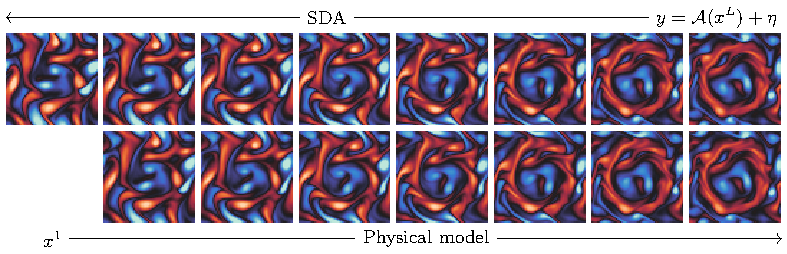
\includegraphics[scale=0.85]{./chapters/sda/figures/circle.pdf}
    \caption{A trajectory consistent with an unlikely observation of the final state $x^L$ is generated with SDA. To verify whether the trajectory is realistic and not hallucinated, we plug its initial state $x^1$ into the physical model and obtain an almost identical trajectory. This indicates that SDA is not simply interpolating between observations, but rather propagates information in a manner consistent with the physical model, even in unlikely scenarios.}
    \label{fig:circle}
\end{figure}

Finally, we investigate whether SDA generalizes to unlikely scenarios. We design an observation process that probes the vorticity of the final state $x^L$ in a circle-shaped sub-domain. Then, we sample a trajectory ($C=1$, $\tau = 0.5$) consistent with a uniform positive vorticity observation in this sub-domain, which is unlikely, but not impossible. The result is discussed in Figure \ref{fig:circle}.

\section{Conclusion}

\paragraph{Impact}
In addition to its contributions to the field of data assimilation, this work presents new technical contributions to the field of score-based generative modeling.

First, we provide new insights on how to exploit conditional independencies (Markov blankets) in sets of random variables to build and train score-based generative models. Based on these findings, we are able to generate/infer simultaneously all the states of arbitrarily long Markov chains $x^{1:L}$, while only training score models on short segments $x^{i-k:i+k}$, thereby reducing the training costs and the amounts of training data required. The decomposition of the global score into local scores additionally allows for better parallelization at inference, which could be significant depending on available hardware. Importantly, the pseudo-blanket approximation \eqref{eq:sda-pseudo-blanket} is not limited to Markov chains, but could be applied to any set of variables $x^{1:L}$, as long as some structure is known.

Second, we motivate and introduce a novel approximation \eqref{eq:sda-likelihood-approx} for the perturbed likelihood $p(y \mid x_t)$, when the likelihood $p(y \mid x)$ is assumed (linear or non-linear) Gaussian. We find that computing the likelihood score $\grad{x_t} \log p(y \mid x_t)$ with this new approximation leads to accurate posterior inference, without the need for stability tricks \cite{chung2023diffusion}. This contribution can be trivially adapted to many tasks such as inpainting, deblurring, super-resolution or inverse problems in scientific fields \cite{song2022solving, adam2022posterior, chung2023diffusion}.

\paragraph{Limitations}
From a computational perspective, even though SDA does not require simulating or differentiating through the physical model, inference remains limited by the speed of the simulation of the reverse SDE. Accelerating sampling in score-based generative models is an active area of research \cite{song2021denoising, liu2022pseudo, zhang2023fast, song2023consistency} with promising results which would be worth exploring in the context of our method.

Regarding the quality of our results, we empirically demonstrate that SDA provides accurate approximations of the whole posterior, especially as $k$ and the number of LMC corrections $C$ increase. However, our approximations \eqref{eq:sda-pseudo-blanket} and \eqref{eq:sda-likelihood-approx} introduce a certain degree of error, which precise impact on the resulting posterior remains to be theoretically quantified. Furthermore, although the Kolmogorov system is high-dimensional (tens of thousands of dimensions) with respect to what is approachable with classical posterior inference methods, it remains small in comparison to the millions of dimensions of some operational DA systems. Whether SDA would scale well to such applications is an open question and will present serious engineering challenges.

Another limitation of our work is the assumption that the dynamics of the system are shared by all trajectories. In particular, if a parametric physical model is used, all trajectories are assumed to share the same parameters. For this reason, SDA is not applicable to settings where fitting the model parameters is also required, or at least not without further developments. Some approaches \cite{archer2015black, maddison2017filtering, naesseth2018variational, lawson2022sixo} tackle this task, but they remain limited to low-dimensional settings. Additionally, if a physical model is used to generate synthetic training data, instead of relying on real data, one can only expect SDA to be as accurate as the model itself. This is a limitation shared by any model-based approach and robust assimilation under model misspecification or distribution shift is left as an avenue for future research.

Finally, posterior inference over entire state trajectories is not always necessary. In forecasting tasks, inferring the current state of the dynamical system is sufficient and likely much less expensive. In this setting, data assimilation reduces to a state estimation problem for which classical methods such as the Kalman filter \cite{kalman1960new} or its nonlinear extensions \cite{wan2000unscented, arasaratnam2009cubature} provide strong baselines. Many deep learning approaches have also been proposed to bypass the physical model entirely and learn instead a generative model of plausible forecasts from past observations only \cite{krishnan2015deep, girin2021dynamical, ravuri2021skilful, lam2023learning}.

\paragraph{Related work}
A number of previous studies have investigated the use of deep learning to improve the quality and efficiency of data assimilation. \textcite{mack2020attentionbased} use convolutional auto-encoders to project the variational data assimilation problem into a lower-dimensional space, which simplifies the optimization problem greatly.
\textcite{frerix2021variational} use a deep neural network to predict the initial state of a trajectory given the observations. This prediction is then used as a starting point for traditional (4D-Var) variational data assimilation methods, which proves to be more effective than starting at random. This strategy is also possible with SDA (using a trajectory sampled with SDA as a starting point) and could help cover multiple modes of the posterior distribution. Finally, \textcite{brajard2020combining} address the problem of simultaneously learning the transition dynamics and estimating the trajectory, when only the observation process is known.

Beyond data assimilation, SDA closely relates to the broader category of sequence models, which have been studied extensively for various types of data, including text, audio, and video. The latest advances demonstrate that score-based generative models achieve remarkable results on the most demanding tasks. \textcite{kong2021diffwave} and \textcite{goel2022its} use score-based models to generate long audio sequences non-autoregressively. \textcite{ho2022video} train a score-based generative model for a fixed number of video frames and use it autoregressively to generate videos of arbitrary lengths. Conversely, our approach is non-autoregressive which allows to generate and condition all elements (frames) simultaneously. Interestingly, as part of their method, \textcite{ho2022video} introduce \enquote{reconstruction guidance} for conditional sampling, which can be seen as a special case of our likelihood approximation \eqref{eq:sda-likelihood-approx} where the observation $y$ is a subset of $x$. Lastly, \textcite{ho2022imagen} generate low-frame rate, low-resolution videos which are then up-sampled temporally and spatially with a cascade \cite{ho2022cascaded} of super-resolution diffusion models. The application of this approach to data assimilation could be worth exploring, although the introduction of arbitrary observation processes seems challenging.

\section*{Acknowledgments}

François Rozet is a research fellow of the F.R.S.-FNRS (Belgium) and acknowledges its financial support.

\clearpage
\section*{References}

\printbibliography[heading=none]

\begin{subappendices}

\clearpage
\section{Unbiased pseudo-blanket approximation} \label{app:sda-unbiased}

For any continuous random variables $a$, $b$ and $c$,
\begin{align*}
    \grad{a} \log p(a, b) & = \frac{1}{p(a, b)} \grad{a} \, p(a, b) \\
    & = \frac{1}{p(a, b)} \grad{a} \int p(a, b, c) \d{c} \\
    & = \int \frac{p(c \mid a, b)}{p(a, b, c)} \grad{a} \, p(a, b, c) \d{c} \\
    & = \mathbb{E}_{p(c \mid a, b)} \big[ \grad{a} \log p(a, b, c) \big] \, .
\end{align*}
Replacing $a$, $b$ and $c$ by $x^i_t$, $x^{\bar{b}_i}_t$ and $x^{\not\in}_t = \{ x^{j}_t : j \neq i \wedge j \not\in \bar{b}_i \}$, respectively, we obtain
\begin{equation*}
    \grad{x^i_t} \log p(x^i_t, x^{\bar{b}_i}_t) = \mathbb{E}_{p(x^{\not\in}_t \mid x^i_t, x^{\bar{b}_i}_t)} \big[ \grad{x^i_t} \log p(x^{1:L}_t) \big] \, ,
\end{equation*}
meaning that $\grad{x^i_t} \log p(x^i_t, x^{\bar{b}_i}_t)$ is the expected value of $\grad{x^i_t} \log p(x^{1:L}_t)$ over $x^{\not\in}_t$. In other words, regardless of the elements or the size of $\bar{b}_i$, $\grad{x^i_t} \log p(x^i_t, x^{\bar{b}_i}_t)$ is an unbiased (exact in expectation) estimate of $\grad{x^i_t} \log p(x^{1:L}_t)$.

\section{On the covariance of $p(x \mid x_t)$} \label{app:sda-covariance}

Assuming a Gaussian prior $p(x)$ with covariance $\Sigma_x$, the covariance $\hat{\Sigma}$ of $p(x \mid x_t)$ takes the form
\begin{align*}
    \hat{\Sigma} & = \Sigma_x - \Sigma_x \left(\Sigma_x + \frac{\sigma_t^2}{\alpha_t^2} I \right)^{-1} \Sigma_x \\
    & = \frac{\sigma_t^2}{\alpha_t^2} Q \Lambda \left(\Lambda + \frac{\sigma_t^2}{\alpha_t^2} I \right)^{-1} Q^{-1}
\end{align*}
where $Q \Lambda Q^{-1}$ is the eigendecomposition of $\Sigma_x$. We observe that for most of the perturbation time $t$, the central diagonal term is close to $\Lambda (\Lambda + I)^{-1}$. We therefore propose the covariance approximation
\begin{align*}
    \hat{\Sigma} & = \frac{\sigma_t^2}{\alpha_t^2} \Gamma
\end{align*}
where $\Gamma = Q \Lambda \left(\Lambda + I\right)^{-1} Q^{-1}$ is a positive semi-definite matrix.

\clearpage
\section{Algorithms} \label{app:sda-aglorithms}

\begin{algorithm}[!h]
    \caption{Estimating the posterior score $\grad{x_t} \log p(x_t \mid y)$} \label{alg:posterior}
    \begin{algorithmic}[1]
        \Function{$s_\phi(x_t, t \mid y)$}{}
            \State $s_x \gets s_\phi(x_t, t)$
            \State $\hat{x} \gets \frac{x_t + \sigma_t^2 \, s_x}{\alpha_t}$
            \State $s_y \gets \grad{x_t} \log \mathcal{N} \left(y \mid \mathcal{A}(\hat{x}), \Sigma_y + \frac{\sigma_t^2}{\alpha_t^2} \Gamma \right)$
            \State \Return{$s_x + s_y$}
        \EndFunction{}
	\end{algorithmic}
\end{algorithm}

\begin{algorithm}[!h]
    \caption{Predictor-Corrector sampling from $s_\phi(x_t, t \mid y)$} \label{alg:sampling}
    \begin{algorithmic}[1]
        \Function{Sample}{$\{t_i\}_{i=0}^N, C, \tau$}
    	    \State{$x_1 \sim \mathcal{N}(0, \Sigma_1)$}
    	    \For{$i = N$ to $1$}
                \State $x_{t_{i-1}} \gets \frac{\alpha_{t_{i-1}}}{\alpha_{t_i}} x_{t_i} + \left( \frac{\alpha_{t_{i-1}}}{\alpha_{t_i}} - \frac{\sigma_{t_{i-1}}}{\sigma_{t_i}} \right) \sigma_{t_i}^2 \, s_\phi(x_{t_i}, t_i \mid y)$
                \For{$j = 1$ to $C$}
                    \State $\epsilon \sim \mathcal{N}(0, I)$
                    \State $s \gets s_\phi(x_{t_{i-1}}, t_{i-1} \mid y)$
                    \State $\delta \gets \tau \frac{\dim(s)}{\| s \|_2^2}$
                    \State $x_{t_{i-1}} \gets x_{t_{i-1}} + \delta \, s + \sqrt{2 \delta} \, \epsilon$
                \EndFor
            \EndFor
            \State \Return{$x_0$}
        \EndFunction{}
	\end{algorithmic}
\end{algorithm}

\clearpage
\section{Experiment details} \label{app:sda-details}

\paragraph{Resources} Experiments were conducted with the help of a cluster of GPUs. In particular, score networks were trained and evaluated concurrently, each on a single GPU with at least \qty{11}{\giga B} of memory.

\paragraph{Lorenz 1963}
We consider two score network architectures: fully-connected local score networks for small $k$ ($k \leq 4$) and fully-convolutional score networks for large $k$ ($k > 4$). Residual blocks \cite{he2016deep}, SiLU \cite{elfwing2018sigmoidweighted} activation functions and layer normalization \cite{ba2016layer} are used for both architecture. The number of blocks in the fully-convolutional architecture controls the value of $k$. We train all score networks for 1024 epochs with the AdamW \cite{loshchilov2019decoupled} optimizer and a linearly decreasing learning rate. Other hyperparameters are provided in Table \ref{tab:hyperparams-lorenz}.

\begin{table}[!h]
    \centering
    \caption{Score network hyperparameters for the Lorenz experiment.}
    \label{tab:hyperparams-lorenz}
    \begin{tabular}{lcc}
        \toprule
        Hyperparameter & $k \leq 4$ & $k > 4$ \\
        \midrule
        Architecture & fully-connected & fully-convolutional \\
        Residual blocks & 5 & $k - 2$ \\
        Features/channels & 256 & 64 \\
        Kernel size & -- & 3 \\
        Activation & SiLU & SiLU \\
        Normalization & LayerNorm & LayerNorm \\
        \midrule
        Optimizer & AdamW & AdamW \\
        Weight decay & \num{e-3} & \num{e-3} \\
        Learning rate & \num{e-3} & \num{e-3} \\
        Scheduler & linear & linear \\
        Epochs & 1024 & 1024 \\
        Batches per epoch & 256 & 256 \\
        Batch size & 256 & 64 \\
        \bottomrule
    \end{tabular}
\end{table}

\paragraph{Kolmogorov flow}
The local score network is a U-Net \cite{ronneberger2015unet} with residual blocks \cite{he2016deep}, SiLU \cite{elfwing2018sigmoidweighted} activation functions and layer normalization \cite{ba2016layer}. This architecture is motivated by the locality of the Navier-Stokes equations, which impose that the evolution of a drop of fluid is determined by its immediate environment. This can be seen as an application of the pseudo-blanket approximation \eqref{eq:sda-pseudo-blanket} to a grid-structured set of random variables. We train the score network for 1024 epochs with the AdamW \cite{loshchilov2019decoupled} optimizer and a linearly decreasing learning rate. Other hyperparameters are provided in Table \ref{tab:hyperparams-kolmogorov}.

\begin{table}[!h]
    \centering
    \caption{Score network hyperparameters for the Kolmogorov experiment.}
    \label{tab:hyperparams-kolmogorov}
    \begin{tabular}{lcc}
        \toprule
        Architecture & U-Net \\
        Residual blocks per level & $(3, 3, 3)$ \\
        Channels per level & $(96, 192, 384)$ \\
        Kernel size & 3 \\
        Padding & circular \\
        Activation & SiLU \\
        Normalization & LayerNorm \\
        \midrule
        Optimizer & AdamW \\
        Weight decay & \num{e-3} \\
        Learning rate & \num{2e-4} \\
        Scheduler & linear \\
        Epochs & 1024 \\
        Batches per epoch & 128 \\
        Batch size & 32 \\
        \bottomrule
    \end{tabular}
\end{table}

\clearpage
\section{Assimilation examples} \label{app:sda-examples}

\vfill{}

\begin{figure}[!h]
    \centering
    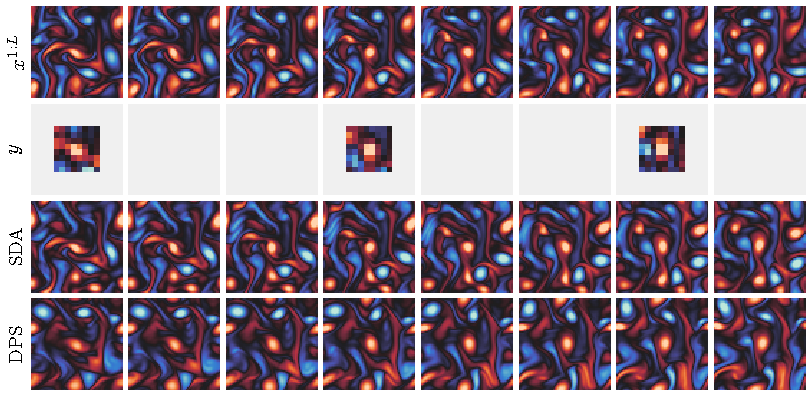
\includegraphics[scale=0.85]{./chapters/sda/figures/extrapolation.pdf}
    \caption{Example of sampled trajectory when the observation is insufficient to identify the original trajectory. The observation is the center of the velocity field every three steps, coarsened to a resolution $8 \times 8$ and perturbed by a small Gaussian noise ($\Sigma_y = 0.01^2 I$). SDA ($C=1$, $\tau=0.5$) identifies the original state where data is sufficient, while generating physically plausible states elsewhere. Replacing SDA's likelihood score approximation with the one of DPS \cite{chung2023diffusion} yields a trajectory less consistent with the observation.}
    \label{fig:extrapolation}
\end{figure}

\vfill{}

\begin{figure}[!h]
    \centering
    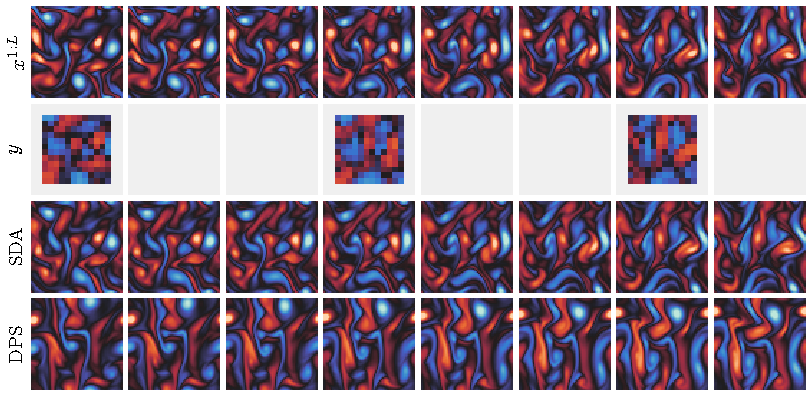
\includegraphics[scale=0.85]{./chapters/sda/figures/saturation.pdf}
    \caption{Example of sampled trajectory when the observation process is non-linear. The observation corresponds to a saturating transformation $x \mapsto \frac{x}{1 + |x|}$ of the vorticity field $\omega$. SDA (512 discretization steps, $C=1$, $\tau=0.5$) identifies the original state where data is sufficient, while generating physically plausible states elsewhere. Replacing SDA's likelihood score approximation with the one of DPS \cite{chung2023diffusion} yields a trajectory inconsistent with the observation.}
    \label{fig:saturation}
\end{figure}

\vfill{}

\begin{figure}[!h]
    \centering
    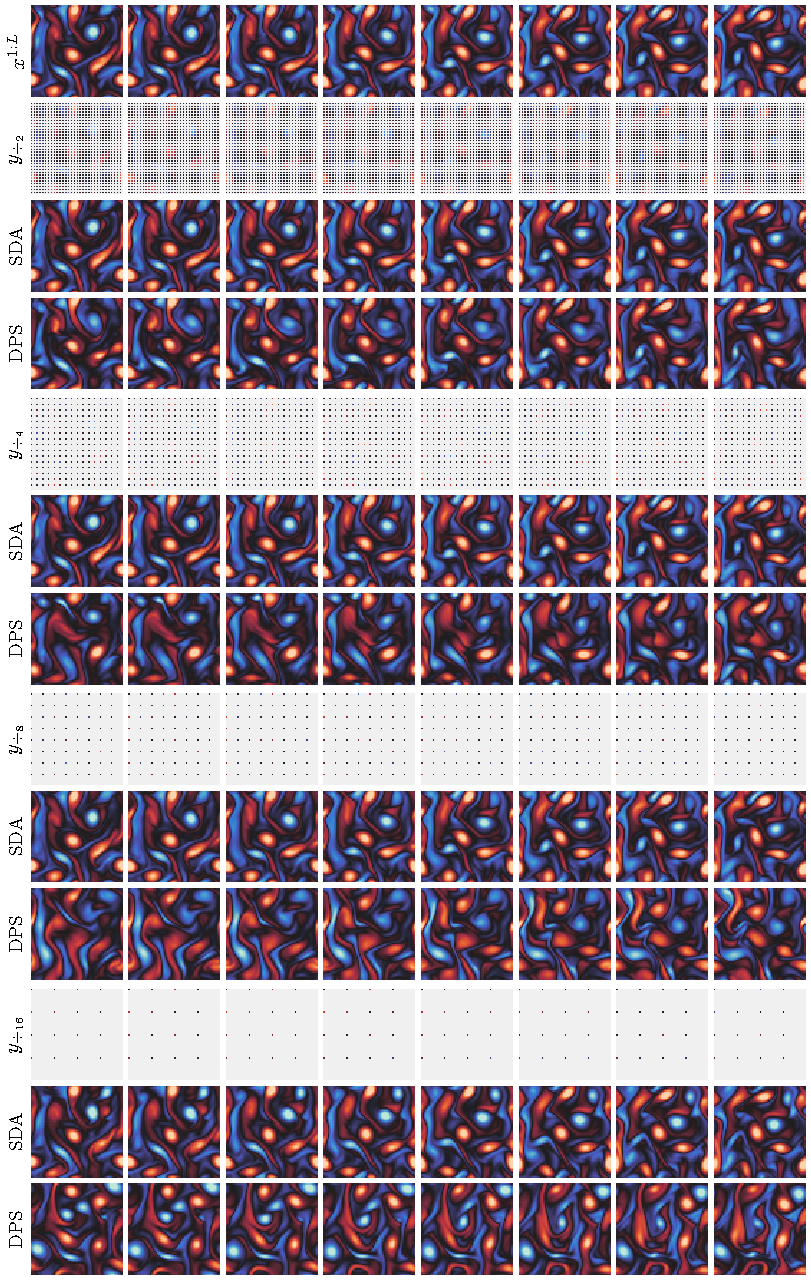
\includegraphics[scale=0.85]{./chapters/sda/figures/subsampling.pdf}
    \caption{Example of sampled trajectories when the observation is spatially sparse. The observation $y_{\div_{n}}$ corresponds to a spatial subsampling of factor $n$ of the velocity field. SDA ($C=1$, $\tau=0.5$) closely recovers the original trajectory for all factors $n$, despite the limited amount of available data. Replacing SDA's likelihood score approximation with the one of DPS \cite{chung2023diffusion} leads to trajectories that are progressively less consistent with the observation as $n$ increases.}
    \label{fig:subsampling}
\end{figure}

\begin{figure}[!h]
    \centering
    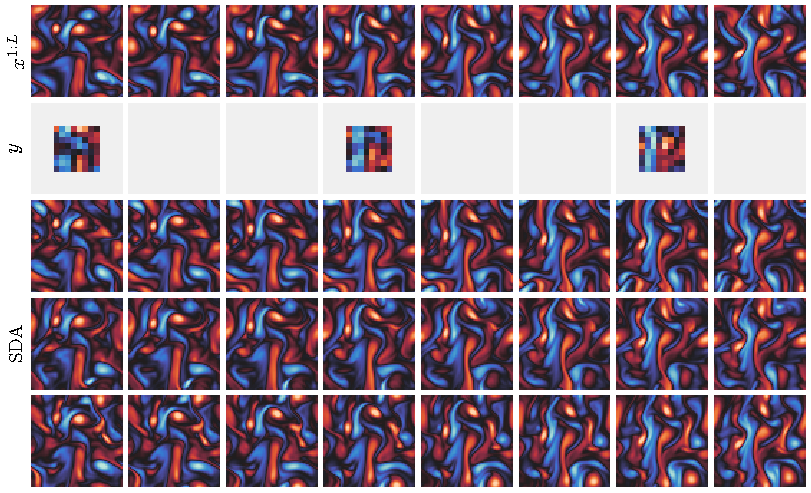
\includegraphics[scale=0.85]{./chapters/sda/figures/extra_bis.pdf}
    \caption{Example of sampled trajectories when the observation is insufficient to identify the original trajectory. The observation is the center of the velocity field every three steps, coarsened to a resolution $8 \times 8$ and perturbed by a small Gaussian noise ($\Sigma_y = 0.01^2 I$). SDA ($C=1$, $\tau=0.5$) identifies the original state where data is sufficient, while generating physically plausible states elsewhere.}
    \label{fig:extrapolation-bis}
\end{figure}

\begin{figure}[!h]
    \centering
    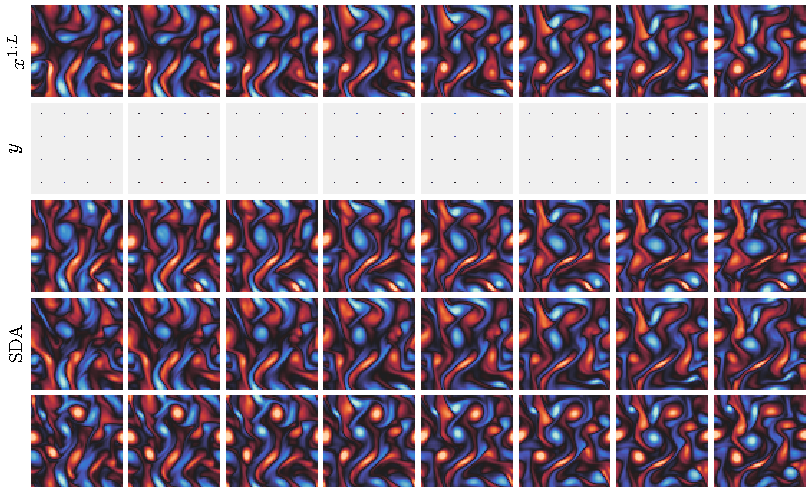
\includegraphics[scale=0.85]{./chapters/sda/figures/sub_bis.pdf}
    \caption{Example of sampled trajectories when the observation is spatially sparse. The observation $y$ corresponds to a spatial subsampling of factor $16$ of the velocity field with medium Gaussian noise ($\Sigma_y = 0.1^2 I$). SDA ($C=1$, $\tau=0.5$) generates trajectories similar to the original, with physically plausible variations.}
    \label{fig:subsampling-bis}
\end{figure}

\begin{figure}[!h]
    \centering
    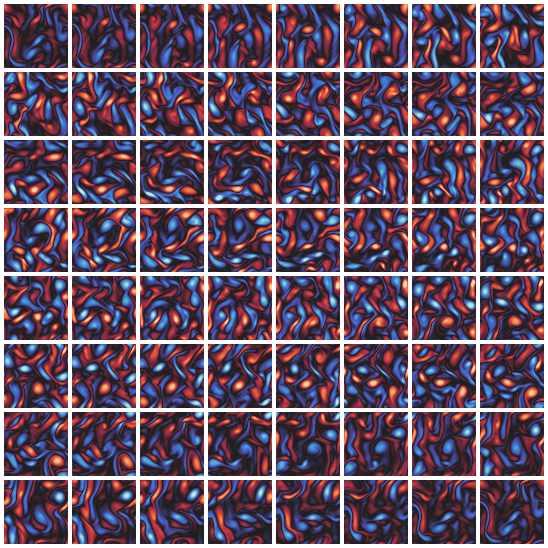
\includegraphics[width=0.85\textwidth]{./chapters/sda/figures/x_loop.png}
    \caption{Example of long ($L=127$) sampled trajectory. Odd states are displayed from left to right and from top to bottom. The observation process probes the difference between the initial and final states and the observation is set to zero, which enforces a looping trajectory ($x^1 \approx x^L$). Note that this scenario is not realistic and will therefore lead to physically implausible trajectories.}
    \label{fig:loop}
\end{figure}

\end{subappendices}

\chapter[Scaling Score-based Data Assimilation]{Scaling Score-based\\Data Assimilation} \label{chap:sda-2lqg}

\begin{quote}
    \begin{flushright}
        \textit{Turbulence is the most important unsolved problem of classical physics.}

        --- Richard Feynman (1964)
    \end{flushright}
\end{quote}

\vspace{2em}

\begin{addendum}{\Large\scshape Addendum}

This chapter appeared previously as

\begin{itemize}[leftmargin=1em]
    \item[] \fullcite{rozet2023scorebaseda}.
\end{itemize}

As the leading author, François came up with the method, conducted the experiments, interpreted the results, and wrote the manuscript. Gilles supervised the project and suggested experiments.

For the version presented in this chapter, we have slightly edited the mathematical notations from the original publication. Notably, the diffusion time notation $x(t)$ has been replaced by the leaner $x_t$, which is more common in nowadays literature and more consistent with the rest of this document. The text itself remains unchanged.

\end{addendum}

\section*{Abstract}

Data assimilation addresses the problem of identifying plausible state trajectories of dynamical systems given noisy or incomplete observations. In geosciences, it presents challenges due to the high-dimensionality of geophysical dynamical systems, often exceeding millions of dimensions. This work assesses the scalability of score-based data assimilation (SDA), a novel data assimilation method, in the context of such systems. We propose modifications to the score network architecture aimed at significantly reducing memory consumption and execution time. We demonstrate promising results for a two-layer quasi-geostrophic model. The code for all experiments is made available at \url{https://github.com/francois-rozet/sda}.

\section{Introduction}

$N$-layer quasi-geostrophic (NLQG) models \cite{cotter2020data} are special cases of the Navier-Stokes equations that have been extensively used to describe the dynamics of oceans and atmospheres. NLQG models consider a stratified fluid of $N$ superimposed layers of constant uniform densities; the layers being stacked according to increasing density. The state of the fluid is fully described by the potential vorticity field $q$ and the velocity fields $(u, v)$ of each layer. In practice, it is necessary to discretize temporally and spatially to solve/integrate the quasi-geostrophic equations, which leads to physical phenomena occurring at a smaller scale than the numerical resolution to be missed \cite{cotter2020data, bolton2019applications, ross2023benchmarking, mangeleer2023ocean}. In the long run, neglecting such phenomena can lead to poor simulations. It is therefore common to simulate such models at high temporal and spatial resolutions to ensure the quality of the simulations, but this comes at a significant computational cost.

Although they make (shallow water) assumptions to neglect some terms of the Navier-Stokes equations, NLGQ models effectively capture the characteristic features of turbulent ocean systems, such as jet streams, mesoscale eddies, and ocean currents. As such, they are good candidates for designing and benchmarking data assimilation (DA) \cite{lorenc1986analysis, ledimet1986variational, tremolet2006accounting, tremolet2007modelerror, fisher2011weakconstraint, carrassi2018data, ecmwf2020ifs} algorithms. Formally, DA targets the problem of inferring the posterior distribution
\begin{equation}
    p(x^{1:L} \mid y) = \frac{p(y \mid x^{1:L})}{p(y)} p(x^1) \prod_{i = 1}^{L - 1} p(x^{i+1} \mid x^i)
\end{equation}
of discrete-time state trajectories $x^{1:L} = (x^1, x^2, \dots, x^L)$ given an observation $y$ resulting from an observation process $p(y \mid x^{1:L})$. In geosciences, the physical model underlying transition dynamics $p(x^{i+1} \mid x^i)$ is typically well known and the observation process is generally formulated as $y = \mathcal{A}(x^{1:L}) + \eta$, where $\mathcal{A}$ is the measurement function and $\eta$ is a stochastic additive term that accounts for instrumental noise and systematic uncertainties.

In this setting, the simulation quality is very important as it strongly impacts the relevance of inference results. Unfortunately, high resolutions rapidly become a computational burden for classical DA algorithms, such as variational methods \cite{lorenc1986analysis, ledimet1986variational, tremolet2006accounting, tremolet2007modelerror, fisher2011weakconstraint} that require to repeatedly differentiate through the physical model, and Monte Carlo methods \cite{evensen1994sequential, liu1998sequential, hamill2006ensemblebased, doucet2011tutorial} that conduct large numbers of simulations.

Conversely, score-based data assimilation (SDA) \cite{rozet2023scorebased}, a novel DA method drawing its roots from score-based generative modeling, only relies on the physical model to generate training data. After training, inference can be carried out without relying on the model and at lower temporal and spatial resolutions. However, applying SDA to (very) high-dimensional systems remains an engineering challenge, which we attempt to address in this work.

\section{Background}

Score-based generative modeling has shown remarkable capabilities, powering many of the latest advances in image, video and audio generation \cite{rombach2022highresolution, ramesh2022hierarchical, saharia2022photorealistic, ho2022video, goel2022its}. In this section, we shortly review score-based generative models and outline how they can be used for solving data assimilation problems with SDA \cite{rozet2023scorebased}.

\paragraph{Continuous-time score-based generative models}
Adopting the notations of \textcite{rozet2023scorebased}, samples $x$ drawn from a distribution $p(x)$ are progressively perturbed through a continuous-time stochastic diffusion process. This process determines a series of marginal distributions $p(x_t)$ from $t=0$ to $t=1$ for which $p(x_0) \approx p(x)$ (clean data) and $p(x_1) \approx \mathcal{N}(0, I)$ (pure noise). By design, the diffusion process can be \enquote{reversed} in order to transform noise $x_1 \sim \mathcal{N}(0, I)$ into data samples $x_0 \sim p(x_0)$. However, this reverse process requires access to the quantity $\grad{x_t} \log p(x_t)$ known as the score of $p(x_t)$.

A score network is a neural network $s_\phi(x_t, t)$ trained -- usually by denoising score matching \cite{hyvarinen2005estimation, vincent2011connection} -- to approximate the score $\grad{x_t} \log p(x_t)$. After training, a score network can be plugged into the reverse process as a substitute for the true score in order to generate data samples from $p(x_0)$. A handy property of score-based models is that, under some assumptions on the likelihood $p(y \mid x)$, it is possible to approximate the posterior score
\begin{equation}
    \grad{x_t} \log p(x_t \mid y) = \grad{x_t} \log p(x_t) + \grad{x_t} \log p(y \mid x_t)
\end{equation}
without retraining the score network $s_\phi(x_t, t)$, and hence to generate data samples from $p(x_0 \mid y)$.

\paragraph{Score-based data assimilation}
In score-based data assimilation, the data we try to model are trajectories $x^{1:L}$ and we therefore approximate the trajectory score $\grad{x^{1:L}_t} \log p(x^{1:L}_t)$. \textcite{rozet2023scorebased} show that an element $\grad{x^{i}_t} \log p(x^{1:L}_t)$ of the trajectory score can be approximated locally by $\grad{x^{i}_t} \log p(x^{i-k:i+k}_t)$ for some $k \geq 1$. They therefore propose to train a local score network $s_\phi(x^{i-k:i+k}_t, t)$ to approximate the score over short segments, and compose this local score at inference to generate arbitrarily long trajectories. In addition, the authors introduce a novel approximation for the likelihood score $\grad{x^{1:L}_t} \log p(y \mid x^{1:L}_t)$ in the assumption of a Gaussian observation process $p(y \mid x^{1:L}) = \mathcal{N}(y \mid \mathcal{A}(x^{1:L}), \Sigma_y)$, which covers many observation scenarios. Finally, to prevent approximation errors from accumulating along the simulation of the reverse process, \textcite{rozet2023scorebased} perform a few Langevin Monte Carlo corrections between each step of the discretized reverse process.

\section{Task}

Although the Kolmogorov system presented in the experiments conducted by \textcite{rozet2023scorebased} is high-dimensional (tens of thousands of dimensions) compared to what is approachable with classical posterior inference methods, it remains small in comparison to the millions of dimensions of some operational DA systems.

In this study, we attempt to perform data assimilation for a two-layer quasi-geostrophic (2LQG) model. We choose a torus-like \qty{1000}{\kilo\meter} periodic domain, discretized into $256 \times 256$ spatial bins. The state is described by the potential vorticity field $q^l$ and the zonal and meridional velocity fields $u^l$ and $v^l$ for each layer $l \in \{1, 2\}$. A state snapshot $x = (q_1, u_1, v_1, q_2, u_2, v_2)$ is therefore a $256 \times 256$ grid with 6 channels, which exceeds the dimensionality of \textcite{rozet2023scorebased}'s Kolmogorov system by a factor 48.

We use the \texttt{pyqg} \cite{abernathey2022pyqg} Python library to solve the quasi-geostrophic equations using pseudo-spectral methods. To ensure the quality of the simulation, the domain is discretized into $512 \times 512$ spatial bins and the integration timestep is set to \qty{15}{min}. We coarsen the simulation to the target resolution ($256 \times 256$) afterwards and separate two snapshots $x^i$ and $x^{i + 1}$ by a day (\qty{24}{h}). To ensure that the system has reached statistical stationarity, that is $p(x^i) = p(x^{i+1})$, it is simulated for 5 years starting from random initial conditions before saving the first state $x^1$ \cite{bolton2019applications, ross2023benchmarking, mangeleer2023ocean}.

\section{Architecture} \label{sec:2lqg-architecture}

The high-dimensionality of the task at hand (and operational DA systems) introduces many engineering challenges. Notably, naively scaling the U-Net \cite{ronneberger2015unet} inspired score network architecture proposed by \textcite{rozet2023scorebased} to our task results in memory consumption exceeding the total memory of a A5000 GPU (\qty{24}{\giga B}) when training on segments, which gets worse at inference on full trajectories. We propose several modifications to the architecture to address these problems, avoiding low-level tricks such as custom CUDA kernels.

First, at inference, except for the extremities of the trajectory, only the $k + 1$-th element of the local score network's output is actually used. The other elements are therefore wasting both memory and compute resources. Instead, we make the score network fully-convolutional in the time axis, such that it can be applied to trajectories of any length. However, we limit its temporal receptive field such that it can still be trained on short segments. To do so, we make all layers 2-D spatial convolutions (no mixing along the time axis) and strategically add a few ($2k$) 1-D temporal convolutions. Assuming the same number of channels per state, this modification roughly reduces the amount of memory consumed and computation performed at inference by a factor $2k + 1$.

Still, training on segments of $256 \times 256$ grid states consumes a lot of memory. To solve this, we combine two ideas: activation checkpointing and inverted bottleneck blocks. Activation checkpointing \cite{chen2016training, gruslys2016memoryefficient} is an automatic differentiation trick that consists in only keeping in memory some intermediate values of the computation graph, instead of all. The missing values are recomputed during the backward pass, effectively trading memory consumption for execution time. Inverted bottleneck blocks \cite{sandler2018mobilenetv2, liu2022convnet} consist in limiting the number of channels of a convolutional network except within residual blocks where the number of channels is expanded to perform non-linear computations and contracted back afterwards. By checkpointing only the intermediate values with a limited number of channels, we are able to reduce memory consumption by \qty{72}{\percent}, while increasing execution time by only \qty{27}{\percent}. A diagram of the architecture incorporating the proposed modifications is provided in Figure \ref{fig:unet}.

\section{Results}

Following \textcite{rozet2023scorebased}, we choose a variance preserving diffusion process for our experiments and simulate the reverse process in 256 evenly spaced discretization steps and one Langevin Monte Carlo correction per step. The score networks are trained once and then evaluated under various observation scenarios.

As described in Section \ref{sec:2lqg-architecture}, the local score network presents a U-Net \cite{ronneberger2015unet} inspired architecture with efficiency-oriented modifications. The temporal receptive field of the score network is such that $k = 4$ and, therefore, it can be trained on segments of length $2k + 1 = 9$ instead of entire trajectories. Using \texttt{pyqg} \cite{abernathey2022pyqg}, we generate 1024 trajectories of 32 state snapshots, which are split into training (\qty{80}{\percent}), validation (\qty{10}{\percent}) and evaluation (\qty{10}{\percent}) sets. For practical reasons, the vorticity and velocity fields (channels) are standardized to have unit variance. We train the score network for 1024 epochs (\qty{48}{h} on a single A5000 GPU) with the AdamW \cite{loshchilov2019decoupled} optimizer and a linearly decreasing learning rate. Further architecture and training details are provided in Appendix \ref{app:2lqg-details}.

We consider a scenario where weather stations placed regularly over the domain measure the local velocities $(u_1, v_1, u_2, v_2)$ every day for a month ($L=32$). We generate an observation $y$ for a trajectory of the evaluation set. Given the observation, we sample three trajectories with SDA and find that they closely resembles the original trajectory, as illustrated in Figure \ref{fig:uniform}. A similar experiment where weather stations are placed randomly upon the domain and with more measurement noise is presented in Figure \ref{fig:random}. In both cases, however, we observe that the generated trajectories exhibit less small-scale details than a simulation, which indicates that the score network does not model the data perfectly. There are several avenues to explore in order to address this issue, such as training for longer with more data or increasing the capacity (more channels or layers) of the score network. Fourier neural operators (FNOs) could be another way to make the network more expressive and have proved to be effective for emulating partial differential equations \cite{li2021fourier, tran2023factorized, mangeleer2023ocean}.

\begin{figure}[!t]
    \centering
    \includegraphics[width=\textwidth]{./chapters/sda_2lqg/compressed/uniform.pdf}
    \caption{Example of sampled trajectories for a spatially sparse observation. States are visualized by their potential vorticity field $q$. Positive values (red) indicate clockwise rotation and negative values (blue) indicate counter-clockwise rotation. The observation $y$ corresponds to a spatial subsampling of factor $16$ of the velocity fields $(u_1, v_1, u_2, v_2)$ with small Gaussian noise ($\Sigma_y = 0.01^2 I$). SDA generates trajectories similar to the original one, despite the limited amount of information available in the observation. The three trajectories present slight physically plausible variations, as expected from sampling from a narrow posterior. We observe that the trajectories exhibit less small-scale details than the original one.}
    \label{fig:uniform}
\end{figure}

Importantly, the three trajectories in Figure \ref{fig:uniform} were generated concurrently on a single A5000 GPU in 18 minutes and using \qty{14}{\giga B} of memory. In comparison, naively scaling the original architecture of \textcite{rozet2023scorebased} would have required roughly 10 times more compute and 20 times more memory. With classical data assimilation algorithms, such as variational \cite{lorenc1986analysis, ledimet1986variational, tremolet2006accounting, tremolet2007modelerror, fisher2011weakconstraint} or Monte Carlo \cite{evensen1994sequential, liu1998sequential, hamill2006ensemblebased, doucet2011tutorial} methods, we estimate that inference would have required the compute equivalent of thousands of simulations, each taking roughly 3 minutes to complete using \texttt{pyqg} \cite{abernathey2022pyqg} on 4 CPU cores. In conclusion, we believe that SDA is ready to be tested in full operational conditions.

\section*{Acknowledgments}

François Rozet is a research fellow of the F.R.S.-FNRS (Belgium) and acknowledges its financial support.

\clearpage
\section*{References}

\printbibliography[heading=none]

\begin{subappendices}

\clearpage
\section{Experiment details} \label{app:2lqg-details}

\paragraph{Resources}
Experiments were conducted with the help of a cluster of GPUs. In particular, score networks were trained and evaluated concurrently, each on a single GPU with 24 GB of memory.

\paragraph{Score network}
The local score network is a U-Net \cite{ronneberger2015unet} with inverted bottleneck residual blocks \cite{he2016deep, sandler2018mobilenetv2, liu2022convnet}, SiLU \cite{elfwing2018sigmoidweighted} activation functions and layer normalization \cite{ba2016layer}. Residual blocks either operate on the temporal axis or the spatial axes (see Section \ref{sec:2lqg-architecture}). Gradient checkpointing \cite{chen2016training, gruslys2016memoryefficient} is applied to the residual blocks to reduce memory consumption. Other hyperparameters are provided in Table \ref{tab:hyperparams-2lqg} and a schematic representation of the architecture is provided in Figure \ref{fig:unet}.

\begin{table}[h]
    \centering
    \caption{Score network hyperparameters for the 2LQG experiment.}
    \label{tab:hyperparams-2lqg}
    \begin{tabular}{lcc}
        \toprule
        Spatial blocks per level & $(3, 3, 3)$ \\
        Channels per level & $(16, 32, 64)$ \\
        Inverted bottleneck factor & 4 \\
        Kernel size & 5 \\
        Padding & circular \\
        Activation & SiLU \\
        Normalization & LayerNorm \\
        \midrule
        Optimizer & AdamW \\
        Weight decay & \num{e-3} \\
        Learning rate & \num{2e-4} \\
        Scheduler & linear \\
        Epochs & 1024 \\
        Batch size & 4 \\
        \bottomrule
    \end{tabular}
\end{table}

\begin{figure}[h]
    \centering
    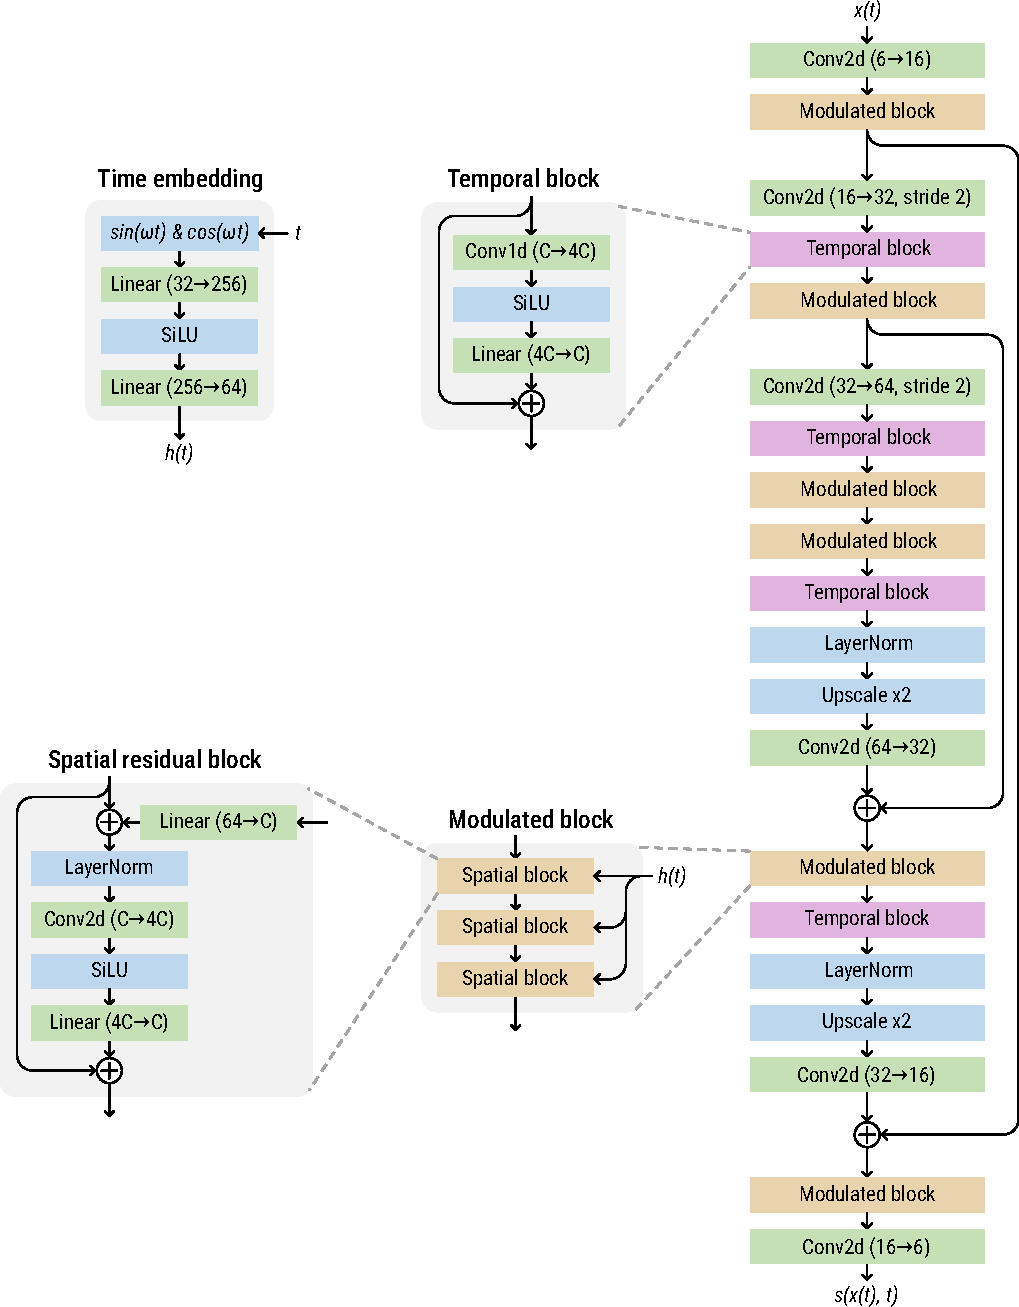
\includegraphics[width=\textwidth]{./chapters/sda_2lqg/figures/diagram.pdf}
    \caption{Schematic representation of the score network architecture. All spatial and temporal blocks are gradient checkpointed to reduce memory consumption.}
    \label{fig:unet}
\end{figure}

\clearpage
\section{Assimilation examples} \label{app:2lqg-example}

\begin{figure}[h]
    \centering
    \includegraphics[width=\textwidth]{./chapters/sda_2lqg/compressed/random.pdf}
    \caption{Example of sampled trajectories for a spatially sparse observation. The observation $y$ corresponds to a random (uniform) sampling of $\pm 80$ bins of the velocity fields $(u_1, v_1, u_2, v_2)$ with medium Gaussian noise ($\Sigma_y = 0.1^2 I$). SDA generates trajectories similar to the original one, despite the limited amount of information available in the observation. The three trajectories present slight physically plausible variations, as expected from sampling from a narrow posterior. We observe that the trajectories exhibit less small-scale details than the original one.}
    \label{fig:random}
\end{figure}

\end{subappendices}

\chapter[Learning Diffusion Priors by Expectation Maximization]{Learning Diffusion Priors by\\Expectation Maximization} \label{chap:diem}

\begin{quote}
    \textit{What we observe is not nature herself, but nature exposed to our method of questioning.}

    \begin{flushright}
        --- Werner Heisenberg (1958) \nocite{heisenberg1958physics}
    \end{flushright}
\end{quote}

\vspace{2em}

\begin{addendum}{\Large\scshape Addendum}

This chapter has previously been published as

\begin{itemize}[leftmargin=1em]
    \item[] \fullcite{rozet2024learning}.
\end{itemize}

The goal of this project, training diffusion models from incomplete and/or noisy data, was proposed by François L. and Gilles. As the leading author, François R. came up with the methods, conducted the experiments, interpreted the results, and wrote the manuscript. Gilles supervised the project, established the link with the EM algorithm, suggested experiments, and participated in the writing and literature review. Gérôme reviewed the manuscript and contributed to the methods through our frequent conversations.

For the version presented in this chapter, we have slightly modified the placement of figures with respect to the original publication. We have also given a name to the main method: diffusion-based expectation-maximization or DiEM, for short. The content remains otherwise unchanged.

\end{addendum}

\section*{Abstract}

Diffusion models recently proved to be remarkable priors for Bayesian inverse problems. However, training these models typically requires access to large amounts of clean data, which could prove difficult in some settings. In this work, we present DiEM, a novel method based on the expectation-maximization algorithm for training diffusion models from incomplete and noisy observations only. Unlike previous works, DiEM leads to proper diffusion models, which is crucial for downstream tasks. As part of our methods, we propose and motivate an improved posterior sampling scheme for unconditional diffusion models. We present empirical evidence supporting the effectiveness of our approach.

\section{Introduction}

Many scientific applications can be formalized as Bayesian inference in latent variable models, where the target is the posterior distribution $p(x \mid y) \propto p(y \mid x) \, p(x)$ given an observation $y \in \mathbb{R}^M$ resulting from a forward process $p(y \mid x)$ and a prior distribution $p(x)$ over the latent variable $x \in \mathbb{R}^N$. Notable examples include gravitational lensing inversion \cite{warren2003semilinear, morningstar2019datadriven, mishra-sharma2022strong}, accelerated MRI \cite{wang2016accelerating, hammernik2018learning, han2020kspace, zbontar2018fastmri, knoll2020fastmri}, unfolding in particle physics \cite{cowan2002survey, blobel2011unfolding}, and data assimilation \cite{ledimet1986variational, tremolet2006accounting, hamill2006ensemblebased, carrassi2018data}. In all of these examples, the observation $y$ alone is either too incomplete or too noisy to recover the latent $x$. Additional knowledge in the form of an informative prior $p(x)$ is crucial for valuable inference.

Recently, diffusion models \cite{sohl-dickstein2015deep, ho2020denoising} proved to be remarkable priors for Bayesian inference, demonstrating both quality and versatility \cite{song2022solving, kawar2021snips, kawar2022denoising, adam2022posterior, chung2023diffusion, song2023pseudoinverseguided, rozet2023scorebased, finzi2023userdefined, boys2023tweedie, zhu2023denoising, dia2023bayesian}. However, to train a diffusion model for the latent $x$, one would typically need a large number of latent realizations, which by definition are not or rarely accessible. This is notably the case in earth and space sciences where the systems of interest can only be probed superficially.

Empirical Bayes (EB) methods \cite{robbins1956empirical, casella1985introduction, carlin2000empirical, efron2014two} offer a solution to the problem of prior specification in latent variable models when only observations $y$ are available. The objective of EB is to find the parameters $\theta$ of a prior model $q_\theta(x)$ for which the evidence distribution $q_\theta(y) = \int p(y \mid x) \, q_\theta(x) \d{x}$ is closest to the empirical distribution of observations $p(y)$. Many EB methods have been proposed over the years, but they remain limited to low-dimensional settings \cite{dagostini1995multidimensional, dockhorn2020density, andreassen2020omnifold, louppe2019adversarial, vandegar2021neural, vetter2024sourcerer} or simple parametric models \cite{efron2016empirical, narasimhan2020deconvolver}.

In this work, our goal is to use diffusion models for the prior $q_\theta(x)$, as they are best-in-class for modeling high-dimensional distributions and enable many downstream tasks, including Bayesian inference. This presents challenges for previous empirical Bayes methods which typically rely on models for which the density $q_\theta(x)$ or samples $x \sim q_\theta(x)$ are differentiable with respect to the parameters $\theta$. Instead, we propose DiEM, an adaptation of the expectation-maximization \cite{hartley1958maximum, dempster1977maximum, wu1983convergence, mclachlan2007em, balakrishnan2017statistical} algorithm where we alternate between generating samples from the posterior $q_\theta(x \mid y)$ and training the prior $q_\theta(x)$ on these samples. As part of our method, we propose an improved posterior sampling scheme for unconditional diffusion models, which we motivate theoretically and empirically.

\section{Diffusion Models} \label{sec:diem-diffusion}

The primary purpose of diffusion models (DMs) \cite{sohl-dickstein2015deep, ho2020denoising}, also known as score-based generative models \cite{song2019generative, song2021scorebased}, is to generate plausible data from a distribution $p(x)$ of interest. Formally, adapting the continuous-time formulation of \textcite{song2021scorebased}, samples $x \in \mathbb{R}^N$ from $p(x)$ are progressively perturbed through a diffusion process expressed as a stochastic differential equation (SDE)
\begin{equation} \label{eq:diem-forward-sde}
    \d{x_t} = f_t \, x_t \d{t} + g_t \d{w_t}
\end{equation}
where $f_t \in \mathbb{R}$ is the drift coefficient, $g_t \in \mathbb{R}_+$ is the diffusion coefficient, $w_t \in \mathbb{R}^N$ denotes a standard Wiener process and $x_t \in \mathbb{R}^N$ is the perturbed sample at time $t \in [0, 1]$. Because the SDE is linear with respect to $x_t$, the perturbation kernel from $x$ to $x_t$ is Gaussian and takes the form
\begin{equation}
    p(x_t \mid x) = \mathcal{N}(x_t \mid \alpha_t \, x, \Sigma_t)
\end{equation}
where $\alpha_t$ and $\Sigma_t = \sigma_t^2 I$ are derived from $f_t$ and $g_t$ \cite{anderson1982reversetime, sarkka2019applied, song2021scorebased, zhang2023fast}. Crucially, the forward SDE \eqref{eq:diem-forward-sde} has an associated family of reverse SDEs \cite{anderson1982reversetime, sarkka2019applied, song2021scorebased, zhang2023fast}
\begin{equation} \label{eq:diem-reverse-sde}
    \d{x_t} = \left[ f_t \, x_t - \frac{1 + \eta^2}{2} g_t^2 \, \grad{x_t} \log p(x_t) \right] \d{t} + \eta \, g_t \d{w_t}
\end{equation}
where $\eta \geq 0$ is a parameter controlling stochasticity. In other words, we can draw noise samples $x_1 \sim p(x_1) \approx \mathcal{N}(0, \Sigma_1)$ and gradually remove the noise therein to obtain data samples $x_0 \sim p(x_0) \approx p(x)$ by simulating Eq. \eqref{eq:diem-reverse-sde} from $t = 1$ to $0$ using an appropriate discretization scheme \cite{song2019generative, ho2020denoising, song2021denoising, song2021scorebased, karras2022elucidating, lipman2023flow, zhang2023fast}. In this work, we adopt the variance exploding SDE \cite{song2019generative} for which $f_t = 0$ and $\alpha_t = 1$.

In practice, the score function $\grad{x_t} \log p(x_t)$ in Eq. \eqref{eq:diem-reverse-sde} is unknown, but can be approximated by a neural network trained via denoising score matching \cite{hyvarinen2005estimation, vincent2011connection}. Several equivalent parameterizations and objectives have been proposed for this task \cite{song2019generative, ho2020denoising, song2021denoising, song2021scorebased, karras2022elucidating, lipman2023flow}. In this work, we adopt the denoiser parameterization $d_\theta(x_t, t)$ and its objective \cite{karras2022elucidating}
\begin{equation} \label{eq:diem-denoiser-objective}
    \arg\min_\theta \mathbb{E}_{p(x) p(t) p(x_t \mid x)} \left[ \lambda_t \left\| d_\theta(x_t, t) - x \right\|_2^2 \right] \, ,
\end{equation}
for which the optimal denoiser is the mean $\mathbb{E}[x \mid x_t]$ of $p(x \mid x_t)$. Importantly, $\mathbb{E}[x \mid x_t]$ is linked to the score function through Tweedie's formula \cite{tweedie1947functions, efron2011tweedies, kim2021noise2score, meng2021estimating}
\begin{equation} \label{eq:diem-optimal-denoiser}
    \mathbb{E}[x \mid x_t] = x_t + \Sigma_t \grad{x_t} \log p(x_t) \, ,
\end{equation}
which allows to use $s_\theta(x_t) = \Sigma_t^{-1} (d_\theta(x_t, t) - x_t)$ as a score estimate in Eq. \eqref{eq:diem-reverse-sde}.

\section{Expectation-Maximization} \label{sec:diem-em}

The objective of the expectation-maximization (EM) algorithm \cite{hartley1958maximum, dempster1977maximum, wu1983convergence, mclachlan2007em, balakrishnan2017statistical} is to find the parameters $\theta$ of a latent variable model $q_\theta(x, y)$ that maximize the log-evidence $\log q_\theta(y)$ of an observation $y$. For a distribution of observations $p(y)$, the objective is to maximize the expected log-evidence \cite{mclachlan2007em, balakrishnan2017statistical} or, equivalently, to minimize the Kullback-Leibler (KL) divergence between $p(y)$ and $q_\theta(y)$. That is,
\begin{align}
    \theta^* & = \arg\max_\theta \mathbb{E}_{p(y)} \big[ \log q_\theta(y) \big] \\
    & = \arg\min_\theta \mathrm{KL} \big( p(y) \, \| \, q_\theta(y) \big) \, .
\end{align}
The key idea behind the EM algorithm is that for any two sets of parameters $\theta_a$ and $\theta_b$, we have
\begin{align}
    \log \frac{q_{\theta_a}(y)}{q_{\theta_b}(y)}
    & = \log \frac{q_{\theta_a}(x, y)}{q_{\theta_b}(x, y)} + \log \frac{q_{\theta_b}(x \mid y)}{q_{\theta_a}(x \mid y)} \\
    & = \mathbb{E}_{q_{\theta_b}(x \mid y)} \left[ \log \frac{q_{\theta_a}(x, y)}{q_{\theta_b}(x, y)} \right] + \mathrm{KL} \big( q_{\theta_b}(x \mid y) \, \| \, q_{\theta_a}(x \mid y) \big) \\
    & \geq \mathbb{E}_{q_{\theta_b}(x \mid y)} \big[ \log q_{\theta_a}(x, y) -  \log q_{\theta_b}(x, y) \big] \, .
\end{align}
This inequality also holds in expectation over $p(y)$. Therefore, starting from arbitrary parameters $\theta_0$, the EM update
\begin{align}
    \theta_{k+1} & = \arg\max_\theta \mathbb{E}_{p(y)} \mathbb{E}_{q_{\theta_k}(x \mid y)} \big[ \log q_\theta(x, y) - \log q_{\theta_k}(x, y)\big] \\
    & = \arg\max_\theta \mathbb{E}_{p(y)} \mathbb{E}_{q_{\theta_k}(x \mid y)} \big[ \log q_\theta(x, y) \big] \label{eq:diem-em-update}
\end{align}
leads to a sequence of parameters $\theta_k$ for which the expected log-evidence $\mathbb{E}_{p(y)} \big[ \log q_{\theta_k}(y) \big]$ is monotonically increasing and converges to a local optimum \cite{wu1983convergence, mclachlan2007em, balakrishnan2017statistical}.

When the expectation in Eq. \eqref{eq:diem-em-update} is intractable, many have proposed to use Monte Carlo approximations instead \cite{wei1990monte, celeux1992stochastic, delyon1999convergence, booth1999maximizing, levine2001implementations, caffo2005ascentbased, jank2006em, ruth2024review}. Previous approaches include Markov chain Monte Carlo (MCMC) sampling, importance sampling, rejection sampling and their variations \cite{levine2001implementations, caffo2005ascentbased, jank2006em, ruth2024review}. A perhaps surprising advantage of Monte Carlo EM (MCEM) algorithms is that they may be able to overcome local optimum traps \cite{celeux1992stochastic, delyon1999convergence}. We refer the reader to \textcite{ruth2024review} for a recent review of MCEM algorithms.

\section{Methods} \label{sec:diem-methods}

Although rarely mentioned in the literature, the expectation-maximization algorithm is a possible solution to the empirical Bayes problem. Indeed, both have the same objective: minimizing the KL between the empirical distribution of observations $p(y)$ and the evidence $q_\theta(y)$. In the empirical Bayes setting, the forward model $p(y \mid x)$ is known and only the parameters of the prior $q_\theta(x)$ should be optimized. In this case, Eq. \eqref{eq:diem-em-update} becomes
\begin{align}
    \theta_{k+1} & = \arg\max_\theta \mathbb{E}_{p(y)} \mathbb{E}_{q_{\theta_k}(x \mid y)} \big[ \log q_\theta(x) + \log p(y \mid x) \big] \\
    & = \arg\max_\theta \mathbb{E}_{p(y)} \mathbb{E}_{q_{\theta_k}(x \mid y)} \big[ \log q_\theta(x) \big] \\
    & = \arg\min_\theta \mathrm{KL} \big( \pi_k(x) \, \| \, q_\theta(x) \big) \label{eq:diem-iter}
\end{align}
where $\pi_k(x) = \int q_{\theta_k}(x \mid y) \, p(y) \d{y}$. Intuitively, $\pi_k(x)$ and therefore $q_{\theta_{k+1}}(x)$ assign more density to latents $x$ which are consistent with observations $y \sim p(y)$ than $q_{\theta_k}(x)$. In this work, we consider a special case of the empirical Bayes problem where each observation $y$ has an associated measurement matrix $A$ and the forward process takes a linear Gaussian form $p(y \mid x, A) = \mathcal{N}(y \mid Ax, \Sigma_y)$. This formulation allows the forward process to be potentially different for each observation $y$. For example, if the position or environment of a sensor changes, the measurement matrix $A$ may also change, which leads to an empirical distribution of pairs $(y, A) \sim p(y, A)$. As a result, $\pi_k(x)$ in Eq. \eqref{eq:diem-iter} becomes $\pi_k(x) = \int q_{\theta_k}(x \mid y, A) \, p(y, A) \d{y}$.

\subsection{Diffusion-based Expectation-Maximization}

Now that our goals and assumptions are set, we present our method to learn a diffusion model $q_\theta(x)$ for the latent $x$ from observations $y$ by expectation-maximization. The idea is to decompose Eq. \eqref{eq:diem-iter} into
\begin{enumerate*}[label=(\roman*)]
    \item generating a dataset of i.i.d. samples from $\pi_k(x)$ and
    \item training $q_{\theta_{k+1}}(x)$ to reproduce the generated dataset.
\end{enumerate*}
We summarize the pipeline in Algorithms \ref{alg:em}, \ref{alg:ddim-sampling} and \ref{alg:mmps}, provided in Appendix \ref{app:diem-algorithms} due to space constraints.

\paragraph{Expectation} To draw from $\pi_k(x)$, we first sample a pair $(y, A) \sim p(y, A)$ and then generate $x \sim q_{\theta_k}(x \mid y, A)$ from the posterior. Unlike previous MCEM algorithms that rely on expensive and hard to tune sampling strategies \cite{levine2001implementations, caffo2005ascentbased, jank2006em, ruth2024review}, the use of a diffusion model enables efficient and embarrassingly parallelizable posterior sampling \cite{chung2023diffusion, song2023pseudoinverseguided, rozet2023scorebased}. However, the quality of posterior samples is critical for the EM algorithm to converge properly \cite{levine2001implementations, caffo2005ascentbased, jank2006em, ruth2024review} and, in this regard, we find previous posterior sampling methods \cite{chung2023diffusion, song2023pseudoinverseguided, rozet2023scorebased, boys2023tweedie, zhu2023denoising} to be unsatisfactory. Therefore, we propose an improved posterior sampling scheme, named moment matching posterior sampling (MMPS), which we present and motivate in Section \ref{sec:diem-mmps}. We evaluate MMPS independently from the context of learning from observations in Appendix \ref{app:diem-mmps-eval}.

\paragraph{Maximization} We parameterize our diffusion model $q_\theta(x)$ by a denoiser network $d_\theta(x_t, t)$ and train it via denoising score matching \cite{hyvarinen2005estimation, vincent2011connection}, as presented in Section \ref{sec:diem-diffusion}. To accelerate the training, we start each iteration with the previous parameters $\theta_k$.

\paragraph{Initialization} An important part of our pipeline is the initial prior $q_0(x)$. Any initial prior leads to a local optimum \cite{wu1983convergence, mclachlan2007em, balakrishnan2017statistical}, but an informed initial prior can reduce the number of iterations until convergence. In our experiments, we take a Gaussian distribution $\mathcal{N}(x \mid \mu_x, \Sigma_x)$ as initial prior and fit its mean and covariance by -- you guessed it! -- expectation-maximization. Fitting a Gaussian distribution by EM is very fast as the maximization step can be conducted in closed-form, especially for low-rank covariance approximations \cite{tipping1999mixtures}.

An alternative we do not explore in this work would be to use a pre-trained diffusion model as initial prior. Pre-training can be conducted on data we expect to be similar to the latents, such as computer simulations or even video games. The more similar, the faster the EM algorithm converges. However, if the initial prior $q_0(x)$ does not cover latents that are otherwise plausible under the observations, the following priors $q_{\theta_k}(x)$ may not cover these latents either. A conservative initial prior is therefore preferable for scientific applications.

\subsection{Moment Matching Posterior Sampling} \label{sec:diem-mmps}

To sample from the posterior distribution $q_\theta(x \mid y) \propto q_\theta(x) \, p(y \mid x)$ of our diffusion prior $q_\theta(x)$, we have to estimate the posterior score $\grad{x_t} \log q_\theta(x_t \mid y)$ and plug it into the reverse SDE \eqref{eq:diem-reverse-sde}. In this section, we propose and motivate an improved approximation for the posterior score. As this contribution is not bound to the context of EM, we temporarily switch back to the notations of Section \ref{sec:diem-diffusion} where our prior is denoted $p(x)$ instead of $q_\theta(x)$.

\paragraph{Diffusion posterior sampling} Thanks to Bayes' rule,\sidenote{\textit{If there be two subsequent events, the probability of the second $\nicefrac{M}{N}$ and\\ the probability of both together $\nicefrac{P}{N}$, and it being first discovered that the second event has also happened, the probability I am right is $\frac{P}{M}$.}\\[1ex] --- Thomas Bayes (1763) \nocite{bayes1763essay}} the posterior score $\grad{x_t} \log p(x_t \mid y)$ can be decomposed into two terms \cite{song2021scorebased, kawar2021snips, song2022solving, chung2023diffusion, song2023pseudoinverseguided, rozet2023scorebased, finzi2023userdefined, boys2023tweedie}
\begin{equation} \label{eq:diem-score-bayes}
    \grad{x_t} \log p(x_t \mid y) = \grad{x_t} \log p(x_t) + \grad{x_t} \log p(y \mid x_t) \, .
\end{equation}
As an estimate of the prior score $\grad{x_t} \log p(x_t)$ is already available via the denoiser $d_\theta(x_t, t)$, the remaining task is to estimate the likelihood score $\grad{x_t} \log p(y \mid x_t)$. Assuming a differentiable measurement function $\mathcal{A}$ and a Gaussian forward process $p(y \mid x) = \mathcal{N}(y \mid \mathcal{A}(x), \Sigma_y)$, \textcite{chung2023diffusion} propose the approximation
\begin{equation} \label{eq:diem-dps}
    p(y \mid x_t) = \int p(y \mid x) \, p(x \mid x_t) \d{x} \approx \mathcal{N} \left(y \mid \mathcal{A}(\mathbb{E}[x \mid x_t]), \Sigma_y \right)
\end{equation}
which allows to estimate the likelihood score $\grad{x_t} \log p(y \mid x_t)$ without training any other network than $d_\theta(x_t, t) \approx \mathbb{E}[x \mid x_t]$. The motivation behind Eq. \eqref{eq:diem-dps} is that, when $\sigma_t$ is small, assuming that $p(x \mid x_t)$ is narrowly concentrated around its mean $\mathbb{E}[x \mid x_t]$ is reasonable. However, this approximation is very poor when $\sigma_t$ is not negligible. Consequently, DPS \cite{chung2023diffusion} is unstable, does not properly cover the support of the posterior $p(x \mid y)$ and often leads to samples $x$ which are inconsistent with the observation $y$ \cite{song2023pseudoinverseguided, rozet2023scorebased, finzi2023userdefined, boys2023tweedie}.

\paragraph{Moment matching} To address these flaws, following studies \cite{song2023pseudoinverseguided, rozet2023scorebased, finzi2023userdefined, boys2023tweedie} take the covariance $\mathbb{V}[x \mid x_t]$ into account when estimating the likelihood score $\grad{x_t} \log p(y \mid x_t)$. Specifically, they consider the Gaussian approximation\sidenote{\textit{Good approximations often lead to better ones.}\\[1ex] --- George Pólya (1977)}
\begin{equation} \label{eq:diem-p_x_xt}
    q(x \mid x_t) = \mathcal{N} \left(x \mid \mathbb{E}[x \mid x_t], \mathbb{V}[x \mid x_t] \right)
\end{equation}
which is closest to $p(x \mid x_t)$ in Kullback-Leibler (KL) divergence \cite{bishop2006pattern}. Then, assuming a linear Gaussian forward process $p(y \mid x) = \mathcal{N}(y \mid A x, \Sigma_y)$, we obtain \cite{bishop2006pattern}
\begin{align} \label{eq:diem-p_y_xt}
    q(y \mid x_t) = \int p(y \mid x) \, q(x \mid x_t) \d{x} = \mathcal{N} \left(y \mid A \mathbb{E}[x \mid x_t], \Sigma_y + A \mathbb{V}[x \mid x_t] A^\top \right)
\end{align}
which allows to estimate the likelihood score $\grad{x_t} \log p(y \mid x_t)$ as
\begin{equation} \label{eq:diem-likelihood-score}
    \grad{x_t} \log q(y \mid x_t) = \grad{x_t} \mathbb{E}[x \mid x_t]^\top A^\top \big(\Sigma_y + A \mathbb{V}[x \mid x_t] A^\top\big)^{-1} \big(y - A \mathbb{E}[x \mid x_t]\big)
\end{equation}
under the assumption that the derivative of $\mathbb{V}[x \mid x_t]$ with respect to $x_t$ is negligible \cite{finzi2023userdefined, boys2023tweedie}. Even with simple heuristics for $\mathbb{V}[x \mid x_t]$, such as $\Sigma_t$ \cite{adam2022posterior} or $(\Sigma_t^{-1} + \Sigma_x^{-1})^{-1}$ \cite{song2023pseudoinverseguided, rozet2023scorebased}, this adaptation leads to significantly more stable sampling and better coverage of the posterior $p(x \mid y)$ than DPS \cite{chung2023diffusion}. However, we find that heuristics lead to overly dispersed posteriors $q(x_t \mid y) \propto p(x_t) \, q(y \mid x_t)$ in the presence of local covariances -- \emph{i.e.} covariances in the neighborhood of $x_t$.

We illustrate this behavior in Figure \ref{fig:manifold} and measure its impact as the Sinkhorn divergence \cite{chizat2020faster, flamary2021pot} between the posteriors $p(x_t \mid y)$ and $q(x_t \mid y)$ when the prior $p(x)$ lies on randomly generated 1-dimensional manifolds \cite{zenke2021remarkable} embedded in $\mathbb{R}^3$. The prior $p(x)$ is modeled as a mixture of isotropic Gaussians centered around points of the manifold, which gives access to $p(x_t)$, $\mathbb{E}[x \mid x_t]$ and $\mathbb{V}[x \mid x_t]$ analytically. The results, presented in Figure \ref{fig:divergence}, indicate that using $\mathbb{V}[x \mid x_t]$ instead of heuristics leads to orders of magnitude more accurate posteriors $q(x_t \mid y)$. We expect this gap to further increase with real high-dimensional data as the latter often lies along low-dimensional manifolds and, therefore, presents strong local covariances.

\begin{figure}[!b]
\begin{minipage}[b]{0.48\textwidth}
    \centering
    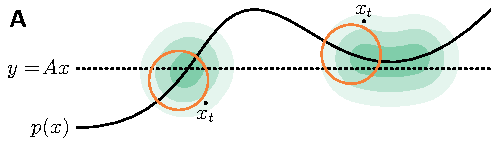
\includegraphics[width=\textwidth]{./chapters/diem/figures/manifold_a.pdf}
    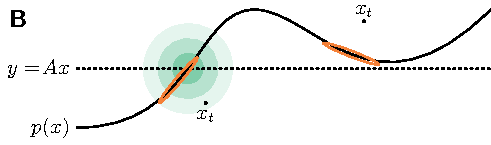
\includegraphics[width=\textwidth]{./chapters/diem/figures/manifold_b.pdf}
    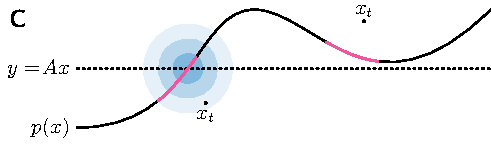
\includegraphics[width=\textwidth]{./chapters/diem/figures/manifold_c.pdf}
    \captionof{figure}{Illustration of the posterior \textcolor{ForestGreen}{$q(x_t \mid y)$} for the Gaussian approximation \textcolor{Orange}{$q(x \mid x_t)$} when the prior $p(x)$ lies on a manifold. Ellipses represent \qty{95}{\percent} credible regions of \textcolor{Orange}{$q(x \mid x_t)$}. (\textbf{\textsf{A}}) With $\Sigma_t$ as heuristic for $\mathbb{V}[x \mid x_t]$, any $x_t$ whose mean \mbox{$\mathbb{E}[x \mid x_t]$} is close to the plane $y =\! Ax$ is considered likely. (\textbf{\textsf{B}}) With $\mathbb{V}[x \mid x_t]$, more regions are correctly pruned. (\textbf{\textsf{C}}) Ground-truth \textcolor{NavyBlue}{$p(x_t \mid y)$} and \textcolor{Rhodamine}{$p(x \mid x_t)$} for reference.}
    \label{fig:manifold}
\end{minipage}%
\hfill%
\begin{minipage}[b]{0.49\textwidth}
    \centering
    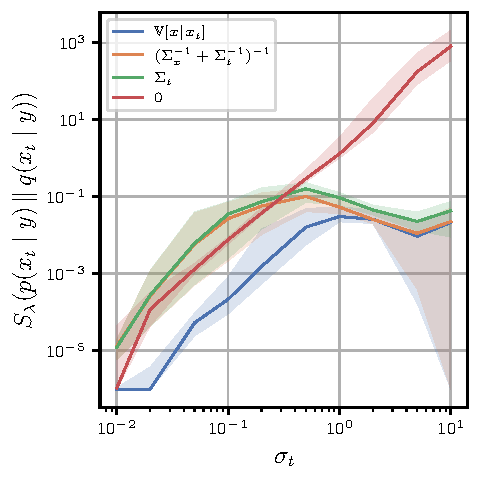
\includegraphics[width=\textwidth]{./chapters/diem/figures/divergence.pdf}%
    \vspace{-0.5em}
    \captionof{figure}{Sinkhorn divergence \cite{chizat2020faster} between the posteriors $p(x_t \mid y)$ and $q(x_t \mid y)$ for different heuristics of $\mathbb{V}[x \mid x_t]$ when the prior $p(x)$ lies on 1-d manifolds embedded in $\mathbb{R}^3$. Lines and shades represent the 25-50-75 percentiles for 64 randomly generated manifolds \cite{zenke2021remarkable} and measurement matrices $A \in \mathbb{R}^{1 \times 3}$. Using $\mathbb{V}[x \mid x_t]$ instead of heuristics leads to orders of magnitude more accurate posteriors $q(x_t \mid y)$. }
    \label{fig:divergence}
\end{minipage}
\end{figure}

Because the MCEM algorithm is sensitive to the accuracy of posterior samples \cite{levine2001implementations, caffo2005ascentbased, jank2006em, ruth2024review}, we choose to estimate $\mathbb{V}[x \mid x_t]$ using Tweedie's covariance formula \cite{tweedie1947functions, efron2011tweedies, kim2021noise2score, meng2021estimating}
\begin{align}
    \mathbb{V}[x \mid x_t] & = \Sigma_t + \Sigma_t \, \grad{x_t}^2 \log p(x_t) \, \Sigma_t \\
    & = \Sigma_t \grad{x_t}^\top \mathbb{E}[x \mid x_t] \approx \Sigma_t \grad{x_t}^\top d_\theta(x_t, t) \, .
\end{align}

\paragraph{Conjugate gradient method} As noted by \textcite{finzi2023userdefined}, explicitly computing and materializing the Jacobian $\grad{x_t}^\top d_\theta(x_t, t) \in \mathbb{R}^{N \times N}$ is intractable in high dimension. Furthermore, even if we had access to $\mathbb{V}[x \mid x_t]$, naively computing the inverse of the matrix $\Sigma_y + A \mathbb{V}[x \mid x_t] A^\top$ in Eq. \eqref{eq:diem-likelihood-score} would still be intractable. Fortunately, we observe that the matrix $\Sigma_y + A \mathbb{V}[x \mid x_t] A^\top$ is symmetric positive definite (SPD) and, therefore, compatible with the conjugate gradient (CG) method \cite{hestenes1952methods}. The CG method is an iterative algorithm to solve linear systems of the form $Mv = b$ where the SPD matrix $M$ and the vector $b$ are known. Importantly, the CG method only requires implicit access to $M$ through an operator that performs the matrix-vector product $Mv$ given a vector $v$. In our case, the linear system to solve is
\begin{align}
    y - A \mathbb{E}[x \mid x_t] & = \big(\Sigma_y + A \mathbb{V}[x \mid x_t] A^\top\big) \, v \\
    & = \Sigma_y v + A \big( \underbrace{v^\top \! A \, \Sigma_t \grad{x_t}^\top \mathbb{E}[x \mid x_t]}_{\text{vector-Jacobian product}} \big)^\top \, .
\end{align}
Within automatic differentiation frameworks \cite{bradbury2018jax, paszke2019pytorch}, the vector-Jacobian product in the right-hand side can be cheaply evaluated. In practice, due to numerical errors and imperfect training, the Jacobian $\grad{x_t}^\top d_\theta(x_t, t) \approx \grad{x_t}^\top \mathbb{E}[x \mid x_t]$ is not always perfectly SPD. Consequently, the CG method becomes unstable after a number of iterations and fails to reach an exact solution. Fortunately, we find that truncating the CG algorithm to very few iterations (1 to 3) already leads to significant improvements over using heuristics for the covariance $\mathbb{V}[x \mid x_t]$. Alternatively, the CG method can be replaced by other iterative algorithms that can solve non-symmetric non-definite linear systems, such as GMRES \cite{saad1986gmres} or BiCGSTAB \cite{vandervorst1992bicgstab}, at the cost of slower convergence.

\section{Results} \label{sec:diem-results}

We conduct three experiments to demonstrate the effectiveness of DiEM. We design the first experiment around a low-dimensional latent variable $x$ whose ground-truth distribution $p(x)$ is known. In this setting, we can use asymptotically exact sampling schemes such as predictor-corrector sampling \cite{song2021scorebased, rozet2023scorebased} or twisted diffusion sampling \cite{wu2023practical} without worrying about their computational cost. This allows us to validate our expectation-maximization pipeline (see Algorithm \ref{alg:em}) in the limit of (almost) exact posterior sampling. The remaining experiments target two benchmarks from previous studies: corrupted CIFAR-10 and accelerated MRI. These tasks provide a good understanding of how our method would perform in typical empirical Bayes applications with limited data and compute.

\subsection{Low-dimensional manifold}

In this experiment, the latent variable $x \in \mathbb{R}^5 \sim p(x)$ lies on a random 1-dimensional manifold embedded in $\mathbb{R}^5$ represented in Figure \ref{fig:manifold-px}. Each observation $y \in \mathbb{R}^2 \sim \mathcal{N}(y \mid Ax, \Sigma_y)$ is the result of a random linear projection of a latent $x$ plus isotropic Gaussian noise ($\Sigma_y = \num{e-4} I$). The rows of the measurement matrix $A \in \mathbb{R}^{2 \times 5}$ are drawn uniformly from the unit sphere $\mathbb{S}^{4}$. We note that observing all push-forward distributions $p(u^\top \! x)$ with $u \in \mathbb{S}^{N - 1}$ of a distribution $p(x)$ in $\mathbb{R}^N$ is sufficient to recover $p(x)$ in theory \cite{bonneel2015sliced, nadjahi2020statistical}. In practice, we generate a finite training set of $2^{16}$ pairs $(y, A)$.

We train a DM $q_\theta(x)$ parameterized by a multi-layer perceptron $d_\theta(x_t, t)$ for $K = 32$ EM iterations. We apply Algorithm \ref{alg:mmps} to estimate the posterior score $\grad{x_t} \log q_{\theta}(x_t \mid y, A)$, but rely on the predictor-corrector \cite{song2021scorebased, rozet2023scorebased} sampling scheme with a large number (4096) of correction steps to sample from the posterior $q_\theta(x \mid y, A)$. We provide additional details such as noise schedule, network architectures, and learning rate in Appendix \ref{app:diem-details}.

As expected, the model $q_{\theta_k}(x)$ converges towards a stationary distribution whose marginals are close to the marginals of the ground-truth $p(x)$, as illustrated in Figure \ref{fig:manifold-evolution}. We attribute the remaining artifacts to finite data and inaccuracies in our sampling scheme.

\begin{figure}[!t]
    \centering
    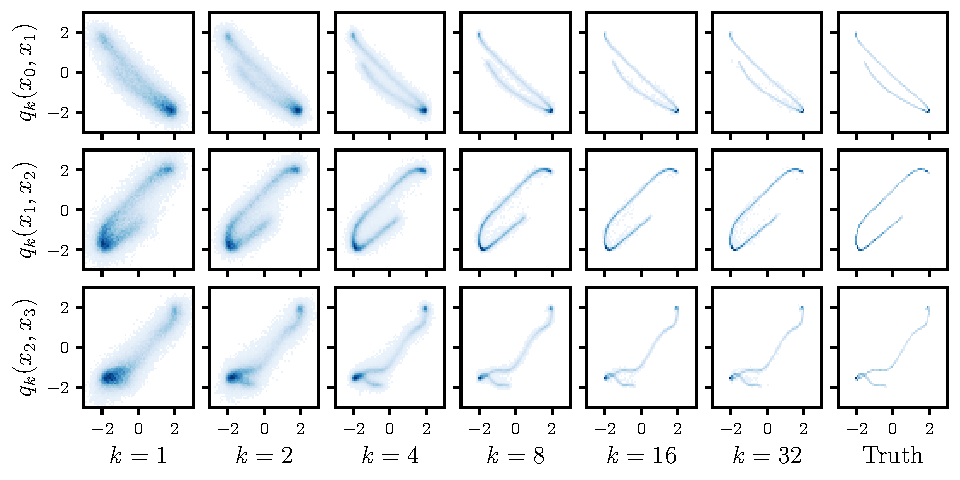
\includegraphics[scale=0.75]{./chapters/diem/figures/manifold_evolution.pdf}
    \caption{Illustration of 2-d marginals of the model $q_{\theta_k}(x)$ along the EM iterations. The initial Gaussian prior $q_0(x)$ leads to a very dispersed first model $q_{\theta_1}(x)$. The EM algorithm gradually prunes the density regions which are inconsistent with observations, until it reaches a stationary distribution. The marginals of the final distribution are close to the marginals of the ground-truth distribution.}
    \label{fig:manifold-evolution}
\end{figure}

\subsection{Corrupted CIFAR-10}

\begin{figure}[!t]
\begin{minipage}[t]{0.50\textwidth}
    \vspace*{0pt}
    \centering
    \resizebox{0.95\textwidth}{!}{%
    \begin{tabular}{l|ccc}
        \toprule
        Method & $\rho$ & FID $\downarrow$ & IS $\uparrow$ \\
        \midrule
        & 0.20 & 11.70 & 7.97 \\
        AmbientDiffusion \cite{daras2023ambient} & 0.40 & 18.85 & 7.45 \\
        & 0.60 & 28.88 & 6.88 \\
        \midrule
        & 0.25 & 5.88 & 8.83 \\
        DiEM w/ Tweedie & 0.50 & 6.76 & 8.75 \\
        & 0.75 & 13.18 & 8.14 \\
        \midrule
        DiEM w/ $(I + \Sigma_t^{-1})^{-1}$ & 0.75 & 39.94 & 7.69 \\
        DiEM w/ $\Sigma_t$ & 0.75 & 118.69 & 4.23 \\
        \bottomrule
    \end{tabular}}
    \vspace{0.25em}
    \captionof{table}{Evaluation of final models trained on corrupted CIFAR-10. DiEM outperforms AmbientDiffusion \cite{daras2023ambient} at similar corruption $\rho$. Using heuristics for $\mathbb{V}[x \mid x_t]$ instead of Tweedie's formula greatly decreases the sample quality.}
    \label{tab:cifar-table}
\end{minipage}%
\hfill%
\begin{minipage}[t]{0.47\textwidth}
    \vspace*{0pt}
    \centering
    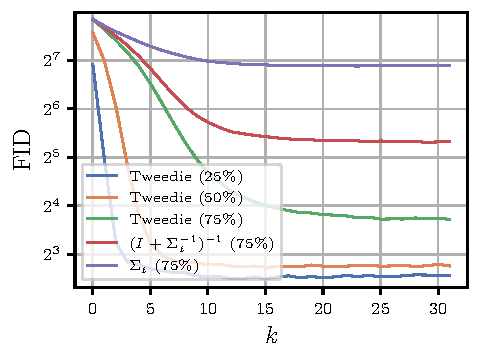
\includegraphics[width=\textwidth]{./chapters/diem/figures/cifar_fid.pdf}%
    \vspace{-0.5em}
    \captionof{figure}{FID of $q_{\theta_k}(x)$ along the EM iterations for the corrupted CIFAR-10 experiment. With less corruption, the EM algorithm converges faster.}
    \label{fig:cifar-fid}
\end{minipage}%
\end{figure}

Following \textcite{daras2023ambient}, we take the \num{50000} training images of the CIFAR-10 \cite{krizhevsky2009learning} dataset as latent variables $x$. A single observation $y$ is generated for each image $x$ by randomly deleting pixels with probability $\rho$. The measurement matrix $A$ is therefore a binary diagonal matrix. We add negligible isotropic Gaussian noise ($\Sigma_y = \num{e-6} I$) for fair comparison with AmbientDiffusion \cite{daras2023ambient} which cannot handle noisy observations.

For each corruption rate $\rho \in \{0.25, 0.5, 0.75\}$, we train a DM $q_\theta(x)$ parameterized by a U-Net \cite{ronneberger2015unet} inspired network $d_\theta(x_t, t)$ for $K = 32$ EM iterations. We apply Algorithm \ref{alg:ddim-sampling} with $T = 256$ discretization steps and $\eta = 1$ to approximately sample from the posterior $q_\theta(x \mid y, A)$. We apply Algorithm \ref{alg:mmps} with several heuristics for $\mathbb{V}[x \mid x_t]$ to compare their results against Tweedie's covariance formula. For the latter, we truncate the conjugate gradient method in Algorithm \ref{alg:cg} to a single iteration.

For each model $q_{\theta_k}(x)$, we generate a set of \num{50000} images and evaluate its Inception score (IS) \cite{salimans2016improved} and Fréchet Inception distance (FID) \cite{heusel2017gans} against the uncorrupted training set of CIFAR-10. We report the results in Table \ref{tab:cifar-table} and Figures \ref{fig:cifar-fid} and \ref{fig:cifar-prior}. At \qty{75}{\percent} of corruption, our method performs similarly to AmbientDiffusion \cite{daras2023ambient} at only \qty{20}{\percent} of corruption. On the contrary, using heuristics for $\mathbb{V}[x \mid x_t]$ leads to poor sample quality.

\begin{figure}[!b]
    \centering
    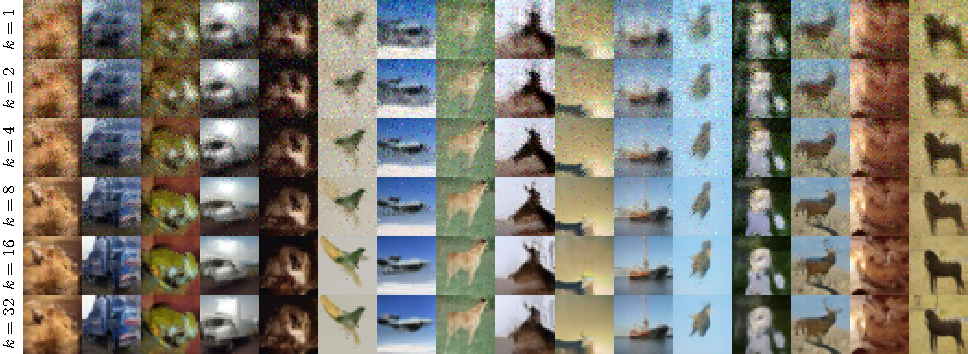
\includegraphics[scale=0.75]{./chapters/diem/figures/cifar_prior_tweedie.pdf}
    \caption{Example of samples from the model $q_{\theta_k}(x)$ along the EM iterations for the corrupted CIFAR-10 experiment with $\rho = 0.75$. We use the deterministic DDIM \cite{song2021denoising} sampling scheme for easier comparison. Generated images become gradually more detailed and less noisy.}
    \label{fig:cifar-prior}
\end{figure}

\subsection{Accelerated MRI}

\begin{figure}[!b]
    \centering
    \includegraphics[scale=0.8]{./chapters/diem/compressed/fastmri_accelerated.pdf}
    \caption{Examples of posterior samples for accelerated MRI using a diffusion prior trained from $k$-space observations only. Posterior samples are detailed and present plausible variations, while remaining consistent with the observation. We provide the zero-filled inverse $\mathcal{F}^{-1}(m \odot y)$ as baseline.}
    \label{fig:fastmri-accelerated}
\end{figure}

Magnetic resonance imaging (MRI) is a non-invasive medical imaging technique used in radiology to inspect the internal anatomy and physiology of the body. MRI measurements of an object are obtained in the frequency domain, also called $k$-space, using strong magnetic fields. However, measuring the entire $k$-space can be time-consuming and expensive. Accelerated MRI \cite{wang2016accelerating, hammernik2018learning, han2020kspace, zbontar2018fastmri, knoll2020fastmri} consists in inferring the scanned object based on partial, possibly randomized and noisy, frequency measurements.

In this experiment, following \textcite{kawar2024gsurebased}, we consider the single-coil knee MRI scans from the fastMRI \cite{zbontar2018fastmri, knoll2020fastmri} dataset. We treat each slice between the 10th and 40th of each scan as an independent latent variable $x$, represented as a $320 \times 320$ gray-scale image. Scans are min-max normalized such that pixel values range between $-2$ and $2$. A single observation $y$ is generated for each slice $x$ by first applying the discrete Fourier transform $\mathcal{F}(x)$ and then a random horizontal frequency sub-sampling mask $m$ with acceleration factor $R = 6$ \cite{jalal2021robust, kawar2024gsurebased}, meaning that a proportion $\nicefrac{1}{R}$ of all frequencies are observed on average. Eventually, we obtain \num{24853} $k$-space observations to which we add isotropic Gaussian noise ($\Sigma_y = \num{e-4} I$) to match \textcite{kawar2024gsurebased}.

Once again, we train a DM $q_\theta(x)$ parameterized by a U-Net \cite{ronneberger2015unet} inspired network $d_\theta(x_t, t)$ for $K = 16$ EM iterations. We apply Algorithm \ref{alg:ddim-sampling} with $T = 64$ discretization steps and $\eta = 1$ to approximately sample from the posterior $q_\theta(x \mid y, A)$ and truncate the conjugate gradient method in Algorithm \ref{alg:cg} to 3 iterations. After training, we employ our final model $q_{\theta_K}(x)$ as a diffusion prior for accelerated MRI. Thanks to our moment matching posterior sampling, we are able to infer plausible scans at acceleration factors up to $R = 32$, as shown in Figure \ref{fig:fastmri-accelerated}. Our samples are noticeably more detailed than the ones of \textcite{kawar2024gsurebased}. We choose not to report the PSNR/SSIM of our samples as these metrics only make sense for regression tasks and unfairly penalize proper generative models \cite{blau2018perceptiondistortion, delbracio2023inversion}. We provide prior samples in Figure \ref{fig:fastmri-prior} and posterior samples for another kind of forward process in Figure \ref{fig:fastmri-crop}.

\section{Related Work} \label{sec:diem-related-work}

\paragraph{Empirical Bayes} A number of previous studies have investigated the use of deep learning to solve the empirical Bayes problem. \textcite{louppe2019adversarial} use adversarial training for learning a prior distribution that reproduces the empirical distribution of observations when pushed through a non-differentiable black-box forward process. \textcite{dockhorn2020density} use normalizing flows \cite{tabak2013family, rezende2015variational} to estimate the prior density by variational inference when the forward process consists of additive noise. \textcite{vandegar2021neural} also use normalizing flows but consider black-box forward processes for which the likelihood $p(y \mid x)$ is intractable. They note that empirical Bayes is an ill-posed problem in that distinct prior distributions may result in the same distribution over observations. \textcite{vetter2024sourcerer} address this issue by targeting the prior distribution of maximum entropy while minimizing the sliced-Wasserstein distance \cite{bonneel2015sliced, nadjahi2020statistical} with the empirical distribution of observations. These methods rely on generative models $q_\theta(x)$ for which the density $q_\theta(x)$ or samples $x \sim q_\theta(x)$ are differentiable with respect to the parameters $\theta$, which is not or hardly the case for diffusion models.

Closer to this work, \textcite{daras2023ambient} and \textcite{kawar2024gsurebased} attempt to train DMs from linear observations only. \textcite{daras2023ambient} consider noiseless observations of the form $y = Ax$ and train a network $d_\theta(A x_t, A, t)$ to approximate $\mathbb{E}[x \mid A x_t]$ under the assumption that $\mathbb{E}[A^\top \! A]$ is full-rank. The authors argue that $\mathbb{E}[x \mid A x_t]$ can act as a surrogate for $\mathbb{E}[x \mid x_t]$. Similarly, \textcite{kawar2024gsurebased} assume Gaussian observations $y \sim \mathcal{N}(y \mid Ax, \Sigma_y)$ and train a network $d_\theta(P x_t, t)$ to approximate $\mathbb{E}[x \mid P x_t]$ under the assumption that $\mathbb{E}[P]$ is full-rank where $P = A^+ \! A$ and $A^+$ is the Moore-Penrose pseudo-inverse of $A$. The authors assume that $d_\theta(P x_t, t)$ can generalize to $P = I$, even if the training data does not contain $P = I$.  In both cases, the trained networks are not proper denoisers approximating $\mathbb{E}[x \mid x_t]$ and cannot reliably parameterize a standard diffusion model, which is problematic for downstream applications. Notably, in the case of Bayesian inference, they require custom posterior sampling schemes such as the one proposed by \textcite{aali2025ambient} for AmbientDiffusion \cite{daras2023ambient} models. Conversely, in this work, we do not make modifications to the denoising score matching objective \cite{hyvarinen2005estimation, vincent2011connection}, which guarantees a proper DM that is compatible with any posterior sampling scheme at every iteration. In addition, we find that DiEM leads to quantitatively and qualitatively better diffusion priors.

In a concurrent work, \textcite{daras2024consistent} propose an algorithm to train DMs from noisy ($A = I$ and $\Sigma_y = \sigma_y^2 I$) data by enforcing the \enquote{consistency} of the denoiser along diffusion paths. They prove that the mean $\mathbb{E}[x \mid x_t]$ is the unique consistent denoiser. Interestingly, this training algorithm also relies on posterior samples, which are easy to obtain thanks to the white noise assumption.

\paragraph{Posterior sampling} Recently, there has been much work on conditional generation using unconditional diffusion models, most of which adopt the posterior score decomposition in Eq. \eqref{eq:diem-score-bayes}. As covered in Section \ref{sec:diem-mmps}, \textcite{chung2023diffusion} propose an analytical approximation for the likelihood score $\grad{x_t} \log p(y \mid x_t)$ when the forward process $p(y \mid x)$ is Gaussian. \textcite{song2023pseudoinverseguided} and \textcite{rozet2023scorebased} improve this approximation by taking the covariance $\mathbb{V}[x \mid x_t]$ into account in the form of simple heuristics. We build upon this idea and replace heuristics with a proper estimate of the covariance $\mathbb{V}[x \mid x_t]$ based on Tweedie's covariance formula \cite{tweedie1947functions, efron2011tweedies, kim2021noise2score, meng2021estimating}. \textcite{finzi2023userdefined} take the same approach, but materialize the matrix $A \mathbb{V}[x \mid x_t] A^\top$ which is intractable in high dimension. \textcite{boys2023tweedie} replace the covariance $\mathbb{V}[x \mid x_t]$ with a row-sum approximation $\operatorname{diag}( e^\top \mathbb{V}[x \mid x_t] )$ where $e$ is the all-ones vector. This approximation is only valid when $\mathbb{V}[x \mid x_t]$ is diagonal, which limits its applicability. Instead, we take advantage of the conjugate gradient method \cite{hestenes1952methods} to avoid materializing $A \mathbb{V}[x \mid x_t] A^\top$. A potential cheaper solution is to train a sparse approximation of $\mathbb{V}[x \mid x_t]$, as proposed by \textcite{peng2024improving}, but this approach is less general and not immediately applicable to any diffusion model.

A parallel line of work \cite{song2023lossguided, bansal2024universal, he2024manifold} extends the conditioning of diffusion models to arbitrary loss terms $\ell(x, y) \propto -\log p(y \mid x)$, for which no reliable analytical approximation of the likelihood score $\grad{x_t} \log p(y \mid x_t)$ exists. \textcite{song2023lossguided} rely on Monte Carlo approximations of the likelihood $p(y \mid x_t) = \int p(y \mid x) \, p(x \mid x_t) \d{x}$ by sampling from a Gaussian approximation of $p(x \mid x_t)$. Conversely, \textcite{he2024manifold} use the mean $\mathbb{E}[x \mid x_t]$ as a point estimate for $p(x \mid x_t)$, but leverage a pre-trained encoder-decoder pair to project the updates of $x_t$ within its manifold. We note that our use of the covariance $\mathbb{V}[x \mid x_t]$ similarly leads to updates tangent to the manifold of $x_t$.

Finally, \textcite{wu2023practical} propose a particle-based posterior sampling scheme that is asymptotically exact in the limit of infinitely many particles as long as the likelihood approximation $q(y \mid x_t)$ -- here named the \emph{twisting} function -- converges to $p(y \mid x)$ as $t$ approaches $0$. Using TDS \cite{wu2023practical} as part of our expectation-maximization pipeline could lead to better results and/or faster convergence, at the cost of computational resources. In addition, the authors note that the efficiency of TDS \cite{wu2023practical} depends on how closely the twisting function approximates the exact likelihood. In this regard, our moment matching Gaussian approximation in Eq. \eqref{eq:diem-p_y_xt} could be a good twisting candidate.

\section{Discussion} \label{sec:diem-discussion}

To the best of our knowledge, we are the first to formalize the training of diffusion models from corrupted observations as an empirical Bayes \cite{robbins1956empirical, casella1985introduction, carlin2000empirical, efron2014two} problem. In this work, we limit our analysis to linear Gaussian forward processes to take advantage of accurate and efficient high-dimensional posterior sampling schemes. This contrasts with typical empirical Bayes methods which target low-dimensional latent spaces and highly non-linear forward processes \cite{dockhorn2020density, andreassen2020omnifold, louppe2019adversarial, vandegar2021neural, vetter2024sourcerer}. In addition, as mentioned in Section \ref{sec:diem-related-work}, these EB methods are not applicable to diffusion models. As such, we choose to benchmark DiEM against similar methods in the diffusion model literature \cite{daras2023ambient, kawar2024gsurebased}, but stress that a proper comparison with previous empirical Bayes methods would be valuable for both communities. We also note that Monte Carlo EM \cite{wei1990monte, celeux1992stochastic, delyon1999convergence, booth1999maximizing, levine2001implementations, caffo2005ascentbased, jank2006em, ruth2024review} can handle arbitrary forward processes $p(y \mid x)$ as long as one can sample from the posterior $q_\theta(x \mid y)$. Therefore, our approach could be adapted to any kind of forward processes in the future. We believe that the works of \textcite{dhariwal2021diffusion} and \textcite{ho2022classifierfree} on diffusion guidance are good avenues for adapting our method to non-linear, non-differentiable, or even black-box forward processes.

From a computational perspective, the iterative nature of DiEM is a drawback compared to previous works \cite{daras2023ambient, kawar2024gsurebased}. Notably, generating enough samples from the posterior can be expensive, although embarrassingly parallelizable. In addition, even though the architecture and training of the model $q_\theta(x)$ itself are simpler than in previous works \cite{daras2023ambient, kawar2024gsurebased}, the sampling step adds a significant amount of complexity, especially as the convergence of our method is sensitive to the quality of posterior samples. In fact, we find that previous posterior sampling methods \cite{chung2023diffusion, song2023pseudoinverseguided, rozet2023scorebased, boys2023tweedie, zhu2023denoising} lead to disappointing results, which motivates us to develop a better one.

As such, moment matching posterior sampling (MMPS) is a byproduct of our work. However, it is not bound to the context of learning from observations and is applicable to any linear inverse problem given a pre-trained diffusion prior. In Appendix \ref{app:diem-mmps-eval}, we evaluate MMPS against previous posterior sampling methods for several linear inverse problems on the FFHQ \cite{karras2019stylebased} dataset. We find that MMPS consistently outperforms previous methods, both qualitatively and quantitatively. MMPS is remarkably stable and requires fewer sampling steps to generate qualitative samples, which largely makes up for its slightly higher step cost.

Finally, as mentioned in Section \ref{sec:diem-related-work}, empirical Bayes is an ill-posed problem in that distinct prior distributions may result in the same distribution over observations. In other words, it is generally impossible to identify \enquote{the} ground-truth distribution $p(x)$ given an empirical distribution of observations $p(y)$. Instead, for a sufficiently expressive diffusion model, our EM method will eventually converge to a prior $q_\theta(x)$ that is consistent with $p(y)$, but generally different from $p(x)$. Following the maximum entropy principle, as advocated by \textcite{vetter2024sourcerer}, is left to future work.

\section*{Acknowledgments}

François Rozet and Gérôme Andry are research fellows of the F.R.S.-FNRS (Belgium) and acknowledge its financial support.

The present research benefited from computational resources made available on Lucia, the Tier-1 supercomputer of the Walloon Region, infrastructure funded by the Walloon Region under the grant no. 1910247. The computational resources have been provided by the Consortium des Équipements de Calcul Intensif (CÉCI), funded by the Fonds de la Recherche Scientifique de Belgique (F.R.S.-FNRS) under the grant no. 2.5020.11 and by the Walloon Region.

MRI data used in the preparation of this article were obtained from the NYU fastMRI Initiative database \cite{knoll2020fastmri, zbontar2018fastmri}. As such, NYU fastMRI investigators provided data but did not participate in analysis or writing of this report. A listing of NYU fastMRI investigators, subject to updates, can be found at \url{https://fastmri.med.nyu.edu/}. The primary goal of fastMRI is to test whether machine learning can aid in the reconstruction of medical images.

\clearpage
\section*{References}

\printbibliography[heading=none]

\begin{subappendices}

\clearpage
\section{Algorithms} \label{app:diem-algorithms}

\begin{algorithm}
    \caption{Expectation-maximization pipeline} \label{alg:em}
    \begin{algorithmic}[1]
        \State Choose an initial prior $q_0(x)$
        \State Initialize the parameters $\theta$ of the denoiser $d_\theta(x_t, t)$
        \For{$k = 1$ to $K$}
            \For{$i = 1$ to $S$}
                \State $y_i, A_i \sim p(y, A)$
                \State $x_i \sim q_{k-1}(x \mid y_i, A_i)$ \Comment{\# Posterior sampling}
            \EndFor
            \Repeat
                \State $i \sim \mathcal{U}(\{1, \dots, S\})$
                \State $t \sim \mathcal{U}(0, 1)$
                \State $z \sim \mathcal{N}(0, I)$
                \State $x_t \gets x_i + \sigma_t \, z$
                \State $\ell \gets \lambda_t \big\| d_\theta(x_t, t) - x_i \big\|^2$ \Comment{\# Denoising score matching}
                \State $\theta \gets \Call{GradientDescent}{\theta, \grad{\theta} \ell}$
            \Until \textbf{convergence}
            \State $\theta_k \gets \theta$
            \State $q_k := q_{\theta_k}$
        \EndFor
        \State \Return{$\theta_K$}
	\end{algorithmic}
\end{algorithm}

\begin{algorithm}
    \caption{DDIM-style posterior sampling} \label{alg:ddim-sampling}
    \begin{algorithmic}[1]
        \State{$x_1 \sim \mathcal{N}(0, \Sigma_1)$}
        \For{$i = T$ to $1$}
            \State $s \gets \nicefrac{i - 1}{T}$
            \State $t \gets \nicefrac{i}{T}$
            \State $\hat{x} \gets x_t + \Sigma_t \, s_{\theta}(x_t \mid y, A)$ \Comment{\# Estimate $\mathbb{E}[x \mid x_t, y, A]$}
            \State $z \sim \mathcal{N}(0, I)$
            \State $\displaystyle x_s \gets \hat{x} + \sigma_s \, \sqrt{1 - \eta \left( 1 - \frac{\sigma_s^2}{\sigma_t^2} \right)} \, \frac{x_t - \hat{x}}{\sigma_t} + \sigma_s \, \sqrt{\eta \left( 1 - \frac{\sigma_s^2}{\sigma_t^2} \right)} \, z$
        \EndFor
        \State \Return{$x_0$}
	\end{algorithmic}
\end{algorithm}

\begin{algorithm}
    \caption{Moment matching posterior score} \label{alg:mmps}
    \begin{algorithmic}[1]
        \Function{}{} $s_{\theta}(x_t \mid y, A)$ \Comment{\# Estimate $\grad{x_t} \log q_\theta(x_t \mid y, A)$}
            \State $\hat{x} \gets d_\theta(x_t, t)$
            \If{Tweedie}
                \State $\Sigma_{x|x_t} \gets \Sigma_t \grad{x_t} d_\theta(x_t, t)^\top$
            \Else
                \State $\Sigma_{x|x_t} \gets \Sigma_t$ or $(I + \Sigma_t^{-1})^{-1}$ or $(\Sigma_x^{-1} + \Sigma_t^{-1})^{-1}$
            \EndIf
            \State $u \gets \left( \Sigma_y + A \Sigma_{x|x_t} A^\top \right)^{-1} (y - A \hat{x})$ \Comment{\# Solve with conjugate gradient method}
            \State $s_{y|x} \gets \grad{x_t} d_\theta(x_t, t) ^\top A^\top u$ \Comment{\# Estimate $\grad{x_t} \log q_\theta(y \mid x_t, A)$}
            \State $s_x \gets \Sigma_t^{-1}(\hat{x} - x_t)$ \Comment{\# Estimate $\grad{x_t} \log q_\theta(x_t)$}
            \State \Return{$s_x + s_{y|x}$}
        \EndFunction
	\end{algorithmic}
\end{algorithm}

\begin{algorithm}
    \caption{Conjugate gradient method} \label{alg:cg}
    \begin{algorithmic}[1]
        \Function{ConjugateGradient}{$A, b, x_0$}
            \State{$r_0 \gets b - A x_0$}
            \State{$p_0 \gets r_0$}
            \For{$i = 0$ to $N - 1$}
                \If{$\| r_i \| \leq \epsilon$}
                    \State \Return{$x_i$}
                \EndIf
                \State $\displaystyle \alpha_i \gets \frac{r_i^\top r_i}{p_i^\top A p_i}$
                \State $x_{i+1} \gets x_i + \alpha_i p_i$
                \State $r_{i+1} \gets r_i - \alpha_i A p_i$
                \State $\displaystyle \beta_i \gets \frac{r_{i+1}^\top r_{i+1}}{r_i^\top r_i}$
                \State $p_{i+1} \gets r_{i+1} + \beta_i p_i$
            \EndFor
            \State \Return{$x_N$}
        \EndFunction
	\end{algorithmic}
\end{algorithm}

\clearpage

\section{Tweedie's formulae} \label{app:diem-tweedie}

\begin{theorem} \label{thm:tweedie}
    For any distribution $p(x)$ and $p(x_t \mid x) = \mathcal{N}(x_t \mid x, \Sigma_t)$, the first and second moments of the distribution $p(x \mid x_t)$ are linked to the score function $\grad{x_t} \log p(x_t)$ through
    \begin{align}
        \mathbb{E} [x \mid x_t] & = x_t + \Sigma_t \, \grad{x_t} \log p(x_t) \\
        \mathbb{V} [x \mid x_t] & = \Sigma_t + \Sigma_t \, \grad{x_t}^2 \log p(x_t) \, \Sigma_t
    \end{align}
\end{theorem}

We provide proofs of Theorem \ref{thm:tweedie} for completeness, even though it is a well known result \cite{tweedie1947functions, efron2011tweedies, kim2021noise2score, meng2021estimating}.

\begin{proof}
    \begin{align*}
        \grad{x_t} \log p(x_t) & = \frac{1}{p(x_t)} \grad{x_t} \, p(x_t) \\
        & = \frac{1}{p(x_t)} \int \grad{x_t} \, p(x, x_t) \d{x} \\
        & = \frac{1}{p(x_t)} \int p(x, x_t) \, \grad{x_t} \log p(x, x_t) \d{x} \\
        & = \int p(x \mid x_t) \, \grad{x_t} \log p(x_t \mid x) \d{x} \\
        & = \int p(x \mid x_t) \, \Sigma_t^{-1} (x - x_t) \d{x} \\
        & = \Sigma_t^{-1} \, \mathbb{E} [x \mid x_t] - \Sigma_t^{-1} \, x_t \qedhere
    \end{align*}
\end{proof}
\begin{proof}
    \begin{align*}
        \grad{x_t}^2 \log p(x_t) & = \grad{x_t} \grad{x_t}^\top \log p(x_t) \\
        & = \grad{x_t} \mathbb{E} [x \mid x_t]^\top \Sigma_t^{-1} - \Sigma_t^{-1} \\
        & = \left( \int \grad{x_t} \, p(x \mid x_t) \, x^\top \d{x} \right) \Sigma_t^{-1} - \Sigma_t^{-1} \\
        & = \left( \int p(x \mid x_t) \grad{x_t} \log \frac{p(x_t \mid x)}{p(x_t)} \, x^\top \d{x} \right) \Sigma_t^{-1} - \Sigma_t^{-1} \\
        & = \left( \int p(x \mid x_t) \, \Sigma_t^{-1} \big(x - \mathbb{E} [x \mid x_t] \big) \, x^\top \d{x} \right) \Sigma_t^{-1} - \Sigma_t^{-1} \\
        & = \Sigma_t^{-1} \Big( \mathbb{E} \left[ x x^\top \mid x_t \right] - \mathbb{E} [x \mid x_t] \, \mathbb{E} [x \mid x_t]^\top \Big) \Sigma_t^{-1} - \Sigma_t^{-1} \\
        & = \Sigma_t^{-1} \, \mathbb{V} [ x \mid x_t ] \, \Sigma_t^{-1} - \Sigma_t^{-1} \qedhere
    \end{align*}
\end{proof}

\newpage
\section{Experiment details} \label{app:diem-details}

All experiments are implemented within the JAX \cite{bradbury2018jax} automatic differentiation framework. The code for all experiments along instructions to obtain the data are made available at \url{https://github.com/francois-rozet/diem}.

\paragraph{Diffusion models} As mentioned in Section \ref{sec:diem-diffusion}, in this work, we adopt the variance-exploding SDE \cite{song2019generative} and the denoiser parameterization \cite{karras2022elucidating}. Following \textcite{karras2022elucidating}, we precondition our denoiser $d_\theta(x_t, t)$ as
\begin{equation}
    d_\theta(x_t, t) = \frac{1}{\sigma_t^2 + 1} x_t + \frac{\sigma_t}{\sqrt{\sigma_t^2 + 1}} h_\theta \left( \frac{x_t}{\sqrt{\sigma_t^2 + 1}}, \log \sigma_t \right)
\end{equation}
where $h_\theta(x, \log \sigma)$ is an arbitrary noise-conditional network. The scalar $\log \sigma$ is embedded as a vector using a sinusoidal positional encoding \cite{vaswani2017attention}. In our experiments, we use an exponential noise schedule
\begin{equation}
    \sigma_t = \exp \big( (1 - t) \log \num{e-3} + t \log \num{e2} \big) \, ,
\end{equation}
loss weights $\lambda_t = \frac{1}{\sigma_t^2} + 1$ and sample $t$ from a Beta distribution $\mathcal{B}(\alpha=3, \beta=3)$ during training.

\paragraph{Low-dimensional manifold} The noise-conditional network $h_\theta(x, \log \sigma)$ is a multi-layer perceptron with 3 hidden layers of 256 neurons and SiLU \cite{elfwing2018sigmoidweighted} activation functions. A layer normalization \cite{ba2016layer} function is inserted after each activation. The input of the network is the concatenation of $x_t$ and the noise embedding vector. We train the network with Algorithm \ref{alg:em} for $K = 32$ EM iterations. Each iteration consists of \num{16384} optimization steps of the Adam \cite{kingma2015adam} optimizer. The optimizer and learning rate are re-initialized after each EM iteration. Other hyperparameters are provided in Table \ref{tab:hyperparams-manifold}.

\begin{table}[h]
    \centering
    \caption{Hyperparameters for the low-dimensional manifold experiment.}
    \label{tab:hyperparams-manifold}
    \begin{tabular}{l|c}
        \toprule
        Architecture & MLP \\
        Input shape & (5) \\
        Hidden features & (256, 256, 256) \\
        Activation & SiLU \\
        Normalization & LayerNorm \\
        \midrule
        Optimizer & Adam \\
        Weight decay & 0.0 \\
        Scheduler & linear \\
        Initial learning rate & \num{1e-3} \\
        Final learning rate & \num{1e-6} \\
        Gradient norm clipping & 1.0 \\
        Batch size & 1024 \\
        Steps per EM iteration & \num{16384} \\
        EM iterations & 32 \\
        \bottomrule
    \end{tabular}
\end{table}

We apply Algorithm \ref{alg:mmps} to estimate the posterior score $\grad{x_t} \log p(x_t \mid y, A)$ and truncate Algorithm \ref{alg:cg} to 3 iterations. We rely on the predictor-corrector \cite{song2021scorebased, rozet2023scorebased} sampling scheme to sample from the posterior $q_\theta(x \mid y, A)$. Following \textcite{rozet2023scorebased}, the predictor is a deterministic DDIM \cite{song2021denoising} step and the corrector is a Langevin Monte Carlo step. We perform 4096 prediction steps, each followed by 1 correction step. At each EM iteration, we generate a single latent $x$ for each pair $(y, A)$.

We generate smooth random manifolds according to a procedure described by \textcite{zenke2021remarkable}. We evaluate the Sinkhorn divergences using the \texttt{POT} \cite{flamary2021pot} package with an entropic regularization factor $\lambda = 1e-3$.

\paragraph{Corrupted CIFAR-10} The noise-conditional network $h_\theta(x, \log \sigma)$ is a U-Net \cite{ronneberger2015unet} with residual blocks \cite{he2016deep}, SiLU \cite{elfwing2018sigmoidweighted} activation functions and layer normalization \cite{ba2016layer}. Each residual block is modulated with respect to the noise $\sigma_t$ in the style of diffusion transformers \cite{peebles2023scalable}. A multi-head self-attention block \cite{vaswani2017attention} is inserted after each residual block at the last level of the U-Net. We train the network with Algorithm \ref{alg:em} for $K = 32$ EM iterations. Each iteration consists of \num{256} epochs over the training set (\num{50000} images). To prevent overfitting, images are augmented with horizontal flips and hue shifts. The optimizer is re-initialized after each EM iteration. Other hyperparameters are provided in Table \ref{tab:hyperparams}.

\begin{table}[h]
    \centering
    \caption{Hyperparameters for the corrupted CIFAR-10 and accelerated MRI experiments.}
    \label{tab:hyperparams}
    \begin{tabular}{l|cc}
        \toprule
        Experiment & corrupted CIFAR-10 & accelerated MRI \\
        \midrule
        Architecture & U-Net & U-Net \\
        Input shape & (32, 32, 3) & (80, 80, 16) \\
        Residual blocks per level & (5, 5, 5) & (3, 3, 3, 3) \\
        Channels per level & (128, 256, 384) & (128, 256, 384, 512) \\
        Attention heads per level & (0, 4, 0) & (0, 0, 0, 4) \\
        Kernel size & 3 & 3 \\
        Activation & SiLU & SiLU \\
        Normalization & LayerNorm & LayerNorm \\
        \midrule
        Optimizer & Adam & Adam \\
        Weight decay & 0.0 & 0.0 \\
        Learning rate & \num{2e-4} & \num{e-4} \\
        Gradient norm clipping & 1.0 & 1.0 \\
        EMA decay & 0.9999 & 0.999 \\
        Dropout & 0.1 & 0.1 \\
        Augmentation & h-flip, hue & h-flip, pad \& crop \\
        Batch size & 256 & 256 \\
        Epochs per EM iteration & 256 & 64 \\
        EM iterations & 32 & 16 \\
        \bottomrule
    \end{tabular}
\end{table}

We apply Algorithm \ref{alg:ddim-sampling} with $T = 256$ discretization steps and $\eta = 1$ to sample from the posterior $q_\theta(x \mid y, A)$. We apply Algorithm \ref{alg:mmps} with several heuristics for $\mathbb{V}[x \mid x_t]$ to compare their results against Tweedie's covariance formula. For the latter, we truncate the conjugate gradient method in Algorithm \ref{alg:cg} to a single iteration. At each EM iteration, we generate a single latent $x$ for each pair $(y, A)$. Each EM iteration (including sampling and training) takes around \qty{4}{\hour} on 4 A100 (40GB) GPUs.

We evaluate the Inception score (IS) \cite{salimans2016improved} and Fréchet Inception distance (FID) \cite{heusel2017gans} of generated images using the \texttt{torch-fidelity} \cite{obukhov2020highfidelity} package.

\paragraph{Accelerated MRI} The noise-conditional network architecture is the same as for the corrupted CIFAR-10 experiment. The $320 \times 320 \times 1$ tensor $x_t$ is reshaped into a $80 \times 80 \times 16$ tensor using pixel shuffling \cite{shi2016realtime} before entering the network. We train the network with Algorithm \ref{alg:em} for $K = 16$ EM iterations. Each iteration consists of \num{64} epochs over the training set ($2 \times \num{24853}$ images). To prevent overfitting, images are augmented with horizontal flips and random crops. The optimizer is re-initialized after each EM iteration. Other hyperparameters are provided in Table \ref{tab:hyperparams}.

We apply Algorithm \ref{alg:ddim-sampling} with $T = 64$ discretization steps and $\eta = 1$ to sample from the posterior $q_\theta(x \mid y, A)$. We truncate the conjugate gradient method in Algorithm \ref{alg:cg} to 3 iterations. At each EM iteration, we generate 2 latents $x$ for each pair $(y, A)$, which acts as data augmentation. Each EM iteration (including sampling and training) takes around \qty{3}{\hour} on 4 A100 (40GB) GPUs.

\clearpage
\section{Additional figures} \label{app:diem-figures}

\begin{figure}[h]
    \centering
    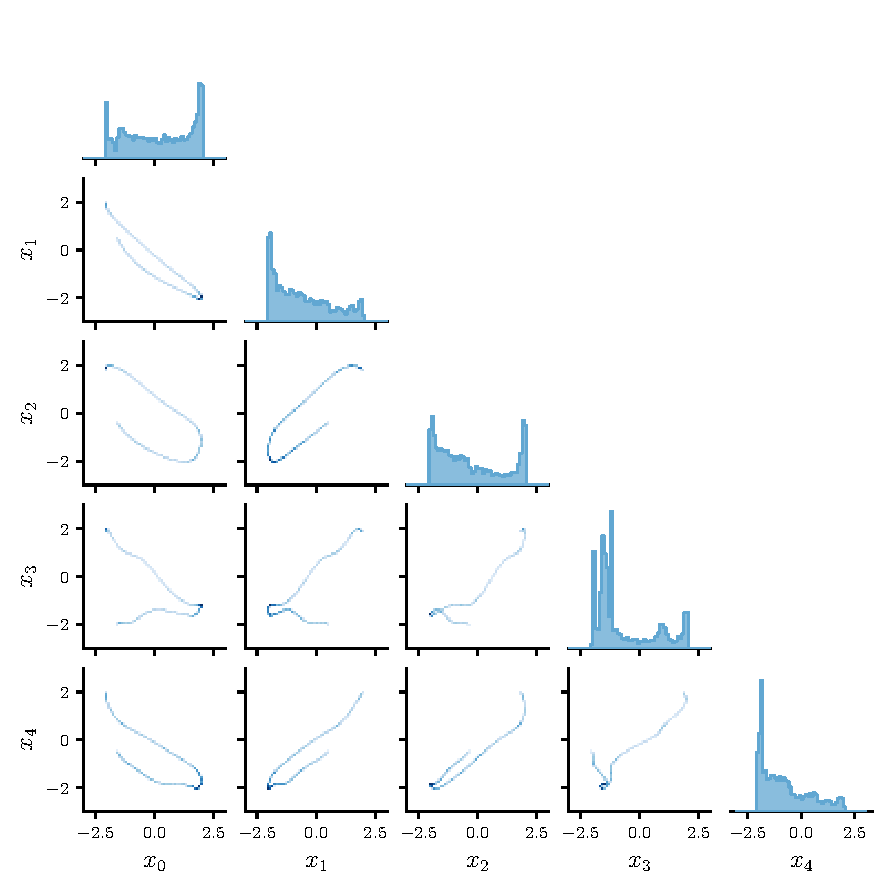
\includegraphics[width=0.9\textwidth]{./chapters/diem/figures/manifold_px.pdf}
    \caption{1-d and 2-d marginals of the ground-truth distribution $p(x)$ used in the low-dimensional manifold experiment. The distribution lies on a random 1-dimensional manifold embedded in $\mathbb{R}^5$.}
    \label{fig:manifold-px}
\end{figure}

% \begin{figure}
%     \centering
%     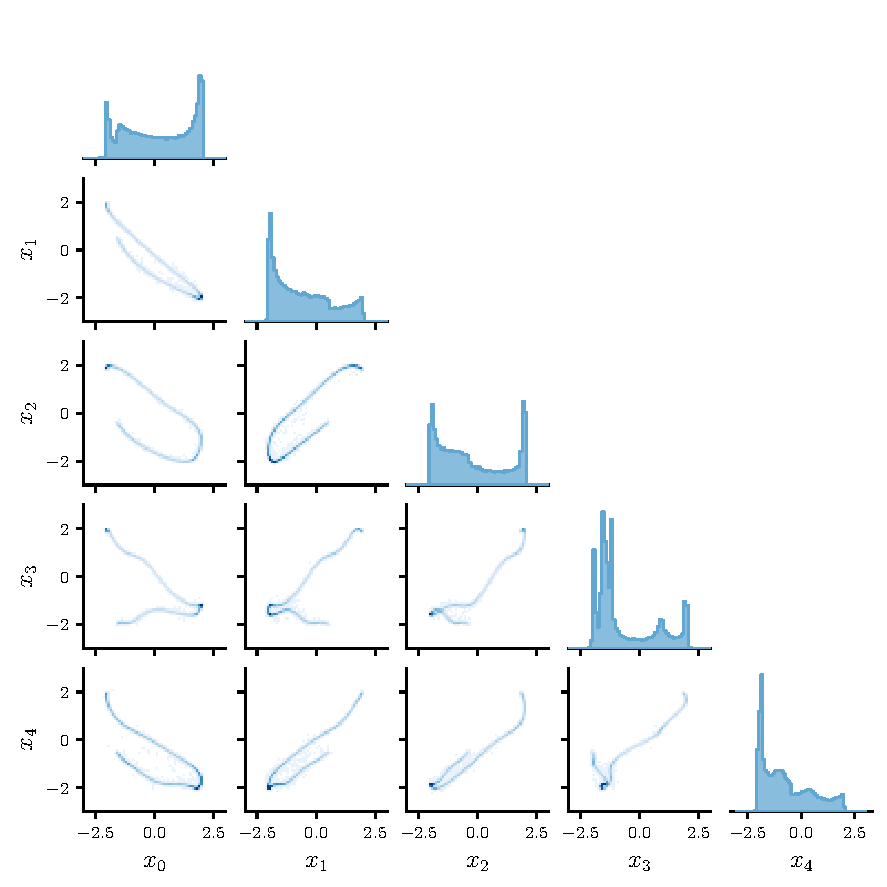
\includegraphics[width=0.8\textwidth]{./chapters/diem/figures/manifold_qx_15.pdf}
%     \caption{Prior learned with our method where $y \in \mathbb{R}^2$ is a random projection, $A \in \mathbb{R}^{2 \times 5}$ is a random projection.}
% \end{figure}

\clearpage

\begin{figure}
    \centering
    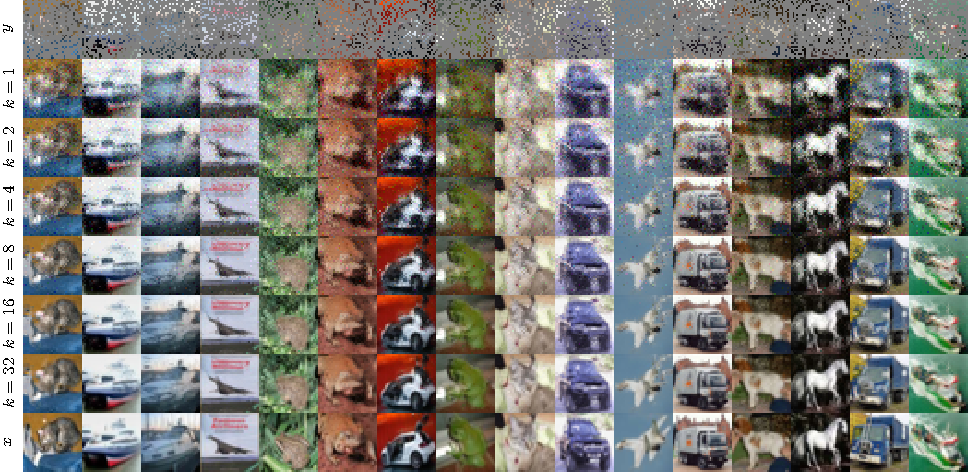
\includegraphics[width=0.95\textwidth]{./chapters/diem/figures/cifar_inpaint_tweedie.pdf}
    \caption{Example of samples from the posterior $q_{\theta_k}(x \mid y)$ along the EM iterations for the CIFAR-10 experiment. The generated images become gradually more detailed and less noisy.}
\end{figure}

\begin{figure}
    \centering
    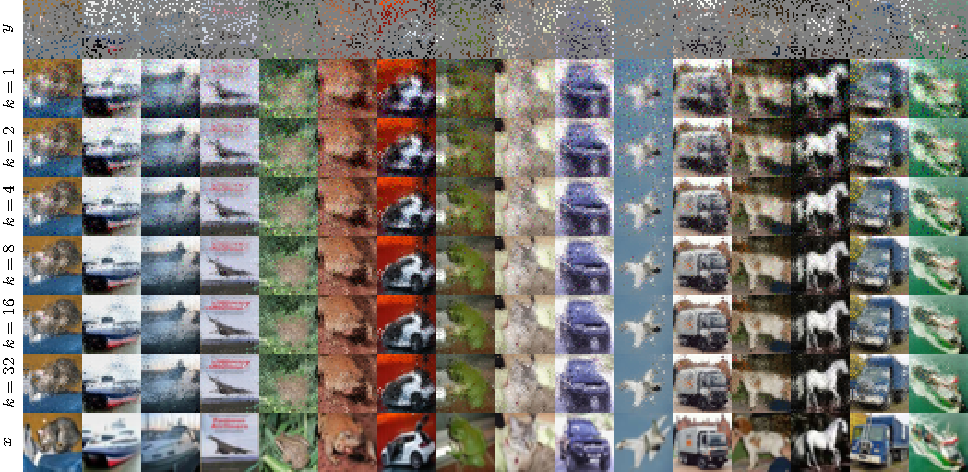
\includegraphics[width=0.95\textwidth]{./chapters/diem/figures/cifar_inpaint_ones.pdf}
    \caption{Example of samples from the posterior $q_{\theta_k}(x \mid y)$ along the EM iterations for the CIFAR-10 experiment when the heuristic $(I + \Sigma_t^{-1})^{-1}$ is used for $\mathbb{V}[x\mid x_t]$. The generated images become gradually more detailed but some noise remains.}
\end{figure}

\begin{figure}
    \centering
    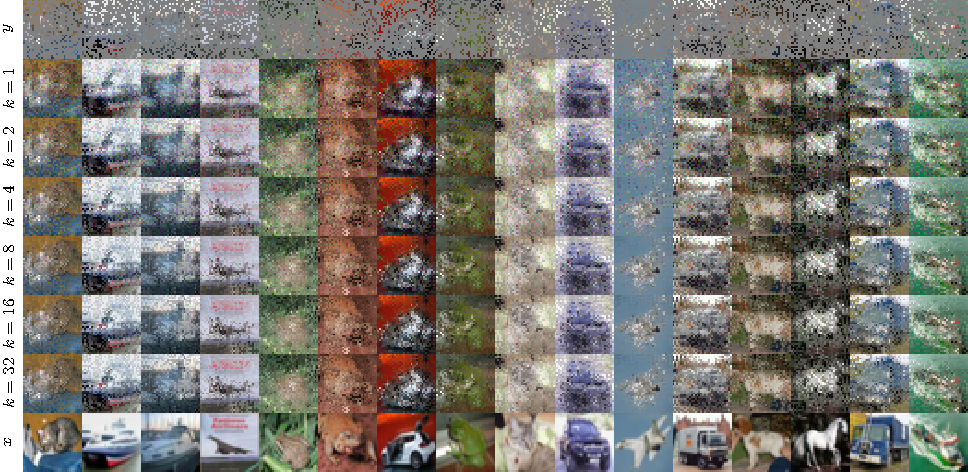
\includegraphics[width=0.95\textwidth]{./chapters/diem/figures/cifar_inpaint_cov_t.pdf}
    \caption{Example of samples from the posterior $q_{\theta_k}(x \mid y)$ along the EM iterations for the CIFAR-10 experiment when the heuristic $\Sigma_t$ is used for $\mathbb{V}[x\mid x_t]$. The generated images remain very noisy.}
\end{figure}

\clearpage

\begin{figure}
    \centering
    \includegraphics[width=0.75\textwidth]{./chapters/diem/compressed/fastmri_x.jpg}
    \caption{Example of scan slices from the fastMRI \cite{zbontar2018fastmri, knoll2020fastmri} dataset.}
    \label{fig:fastmri-x}
\end{figure}

\begin{figure}
    \centering
    \includegraphics[width=0.75\textwidth]{./chapters/diem/compressed/fastmri_y.jpg}
    \caption{Example of $k$-space sub-sampling observations with acceleration factor $R = 6$ for the accelerated MRI experiment. We represent each observation by its zero-filled inverse, where missing frequencies are set to zero before taking the inverse discrete Fourier transform.}
    \label{fig:fastmri-y}
\end{figure}

\begin{figure}
    \centering
    \includegraphics[width=0.75\textwidth]{./chapters/diem/compressed/fastmri_prior.jpg}
    \caption{Example of samples from the final model $q_{\theta_k}(x)$ for the accelerated MRI experiment. The samples present varied and coherent global structures. Samples seem slightly less sharp than real scans (see Figure \ref{fig:fastmri-x}), but do not present artifacts typical to unresolved frequencies (see Figure \ref{fig:fastmri-y}).}
    \label{fig:fastmri-prior}
\end{figure}

\begin{figure}
    \centering
    \includegraphics[width=0.9\textwidth]{./chapters/diem/compressed/fastmri_crop.pdf}
    \caption{Examples of posterior samples using a diffusion prior trained from $k$-space observations only. The forward process crops the latent $x$ to a centered $160 \times 160$ window. Moment matching posterior sampling is used to sample from the posterior. Samples are consistent with the ground-truth where observed, but present plausible variations elsewhere.}
    \label{fig:fastmri-crop}
\end{figure}

\begin{figure}
    \centering
    \includegraphics[width=0.75\textwidth]{./chapters/diem/compressed/fastmri_prior_collapse_1.jpg}
    \caption{Example of samples from the model $q_{\theta_k}(x)$ after $k = 2$ EM iterations for the accelerated MRI experiment when the heuristic $(I + \Sigma_t^{-1})^{-1}$ is used for $\mathbb{V}[x\mid x_t]$. The samples start to present vertical artifacts due to poor sampling.}
\end{figure}

\begin{figure}
    \centering
    \includegraphics[width=0.75\textwidth]{./chapters/diem/compressed/fastmri_prior_collapse_3.jpg}
    \caption{Example of samples from the model $q_{\theta_k}(x)$ after $k = 4$ EM iterations for the accelerated MRI experiment when the heuristic $(I + \Sigma_t^{-1})^{-1}$ is used for $\mathbb{V}[x\mid x_t]$. The artifacts introduced by the poor sampling get amplified at each iteration, leading to a total collapse after few iterations.}
\end{figure}

\clearpage

\section{Evaluation of MMPS} \label{app:diem-mmps-eval}

In this section, we evaluate moment matching posterior sampling (MMPS) presented in Section \ref{sec:diem-mmps} independently from the context of learning from observations. The code is available at \url{https://github.com/francois-rozet/mmps-benchmark}.

\paragraph{Tasks} We consider four linear inverse problems on the $256 \times 256$ FFHQ \cite{karras2019stylebased} dataset.
\begin{enumerate*}[label=(\roman*)]
    \item For box inpainting, we mask out a randomly positioned $128 \times 128$ square of pixels and add a large amount of noise ($\sigma_y = 1$).
    \item For random inpainting, we randomly delete pixels with $\qty{98}{\percent}$ probability and add a small amount of noise ($\sigma_y = 0.01$).
    \item For motion deblur, we apply a randomly generated $61 \times 61$ motion blur kernel and add a medium amount of noise ($\sigma_y = 0.1$).
    \item For super resolution, we apply a $4 \times$ bicubic downsampling and add a medium amount of noise ($\sigma_y = 0.1$).
\end{enumerate*}

\paragraph{Methods} For all inverse problems, we use the pre-trained diffusion model provided by \textcite{chung2023diffusion} as diffusion prior. We adapt and extend the DPS \cite{chung2023diffusion} codebase to support MMPS as well as DiffPIR \cite{zhu2023denoising}, $\Pi$GDM \cite{song2023pseudoinverseguided} and TMPD \cite{boys2023tweedie}. We use the DDIM \cite{song2021denoising} sampler with $\eta = 1$ for all methods, which is equivalent to the DDPM \cite{ho2020denoising} sampler. We fine-tune the hyperparameters of DPS ($\zeta' = 0.5$) and DiffPIR ($\lambda = 8.0$) to have the best results across the four tasks. With MMPS, we find that the Jacobian of the pre-trained model provided by \textcite{chung2023diffusion} is strongly non-symmetric and non-definite for large $\sigma_t$, which leads to unstable conjugate gradient (CG) \cite{hestenes1952methods} iterations. We therefore replace the CG solver with the GMRES \cite{saad1986gmres} solver, which can solve non-symmetric non-definite linear systems.

\paragraph{Protocol} We generate one observation per inverse problem for 100 images\footnotemark{} of the FFHQ \cite{karras2019stylebased} dataset. We generate a sample for each observation with all considered posterior sampling methods. All methods are executed with the same random seed. We compute three standard image reconstruction metrics -- LPIPS \cite{zhang2018unreasonable}, PSNR and SSIM \cite{wang2004image} -- for each sample and report their average in Table \ref{tab:quantitative}. We present generated samples for each inverse problem in Figures \ref{fig:qualitative-mmps}, \ref{fig:qualitative-dps-diffpir} and \ref{fig:qualitative-pgdm-tmpd}.

\footnotetext{\textcite{chung2023diffusion} do not indicate which subset of FFHQ \cite{karras2019stylebased} was used to train their model. Without further information, we choose to use the first 100 images for evaluation, which could lead to biased metrics if the diffusion prior was trained on them. However, since we use the same diffusion prior for all posterior sampling methods, the evaluation remains fair.}

As a side note, we emphasize that reconstruction metrics do not necessarily reflect the accuracy of the inferred posterior distribution, which we eventually care about. For example, PSNR and SSIM \cite{wang2004image} favor smooth predictions such as the mean $\mathbb{E}[x \mid y]$ over actual samples from the posterior $p(x \mid y)$. Conversely, LPIPS \cite{zhang2018unreasonable} favors predictions which are \emph{perceptually} similar to the reference, even if they are distorted. In general, it is impossible to simultaneously optimize for all reconstruction metrics \cite{blau2018perceptiondistortion, delbracio2023inversion}.

\paragraph{Results} MMPS consistently outperforms all baselines, both qualitatively and quantitatively. As expected, performing more solver iterations improves the sample quality, especially when the Gram matrix $A A^\top$ is strongly non-diagonal, which is the case for the motion deblur task. However, the improvement shows rapidly diminishing returns, as the difference between 1 and 3 iterations is much larger than between 3 and 5. MMPS is also remarkably stable with respect to the number of sampling steps in contrast to DPS \cite{chung2023diffusion}, DiffPIR \cite{zhu2023denoising} and $\Pi$GDM \cite{song2023pseudoinverseguided} which are sensitive to the number of steps and choice of hyperparameters. Finally, MMPS requires fewer sampling steps to reach the same image quality as previous methods, which largely makes up for its slightly higher step cost.

\begin{table}
    \renewcommand{\arraystretch}{1.25}
    \addtolength{\tabcolsep}{-0.25em}
    \centering
    \caption{Quantitative evaluation of MMPS with 1, 3 and 5 solver iterations.}
    \resizebox{\textwidth}{!}{%
    \begin{tabular}{ll|ccc|ccc|ccc|ccc}
        \toprule
        & & \multicolumn{3}{c|}{\bfseries Box inpainting} & \multicolumn{3}{c|}{\bfseries Random inpainting} & \multicolumn{3}{c|}{\bfseries Motion deblur} & \multicolumn{3}{c}{\bfseries Super resolution} \\
        Method & Steps & LPIPS $\downarrow$ & PSNR $\uparrow$ & SSIM $\uparrow$ & LPIPS $\downarrow$ & PSNR $\uparrow$ & SSIM $\uparrow$ & LPIPS $\downarrow$ & PSNR $\uparrow$ & SSIM $\uparrow$ & LPIPS $\downarrow$ & PSNR $\uparrow$ & SSIM $\uparrow$ \\
        \midrule
        DiffPIR \cite{zhu2023denoising} & 10 & 0.33 & 19.17 & 0.50 & 0.78 & 10.97 & 0.32 & 0.24 & 24.54 & 0.72 & 0.20 & 26.63 & 0.78 \\
        DiffPIR \cite{zhu2023denoising} & 100 & 0.30 & 18.15 & 0.54 & 0.68 & 10.26 & 0.25 & 0.19 & 23.97 & 0.70 & 0.17 & 25.24 & 0.73 \\
        DiffPIR \cite{zhu2023denoising} & 1000 & 0.33 & 17.39 & 0.49 & 0.74 & 9.51 & 0.21 & 0.17 & 23.55 & 0.67 & 0.15 & 24.72 & 0.70 \\
        DPS \cite{chung2023diffusion} & 10 & 0.64 & 10.41 & 0.34 & 0.58 & 12.68 & 0.43 & 0.75 & 8.63 & 0.27 & 0.58 & 12.01 & 0.41 \\
        DPS \cite{chung2023diffusion} & 100 & 0.38 & 16.82 & 0.50 & 0.39 & 16.66 & 0.49 & 0.29 & 19.75 & 0.57 & 0.35 & 18.29 & 0.54 \\
        DPS \cite{chung2023diffusion} & 1000 & 0.22 & 21.01 & 0.64 & 0.19 & 21.90 & 0.66 & 0.18 & 22.91 & 0.66 & 0.16 & 25.02 & 0.72 \\
        $\Pi$GDM \cite{song2023pseudoinverseguided} & 10 & 0.40 & 18.94 & 0.61 & 0.59 & 11.28 & 0.40 & 0.25 & 25.83 & 0.76 & 0.25 & 26.42 & 0.77 \\
        $\Pi$GDM \cite{song2023pseudoinverseguided} & 100 & 0.44 & 18.23 & 0.47 & 0.39 & 17.03 & 0.48 & 0.25 & 22.37 & 0.61 & 0.15 & 25.63 & 0.71 \\
        $\Pi$GDM \cite{song2023pseudoinverseguided} & 1000 & 0.81 & 14.80 & 0.31 & \textbf{0.14} & 22.32 & 0.69 & 1.06 & 13.12 & 0.21 & 0.64 & 18.41 & 0.29 \\
        TMPD \cite{boys2023tweedie} & 10 & 0.36 & 19.90 & 0.64 & 0.59 & 11.08 & 0.40 & 0.27 & 25.28 & 0.74 & 0.26 & 26.07 & 0.76 \\
        TMPD \cite{boys2023tweedie} & 100 & 0.27 & 19.86 & 0.64 & 0.58 & 10.73 & 0.31 & 0.17 & \underline{26.22} & 0.76 & 0.17 & 26.79 & 0.77 \\
        TMPD \cite{boys2023tweedie} & 1000 & 0.25 & 19.53 & 0.62 & 0.68 & 9.98 & 0.25 & 0.14 & 25.91 & 0.74 & 0.14 & 26.53 & 0.76 \\
        \midrule
        MMPS (1) & 10 & 0.27 & 21.19 & \underline{0.68} & 0.26 & 22.41 & 0.69 & 0.33 & 22.12 & 0.66 & 0.24 & 26.94 & 0.78 \\
        MMPS (1) & 100 & \underline{0.20} & 21.19 & 0.67 & 0.18 & 22.18 & 0.69 & 0.20 & 23.92 & 0.71 & 0.15 & 27.32 & \underline{0.79} \\
        MMPS (1) & 1000 & \textbf{0.19} & 20.77 & 0.64 & 0.18 & 21.94 & 0.66 & 0.16 & 23.83 & 0.69 & \underline{0.12} & 26.92 & 0.77 \\
        MMPS (3) & 10 & 0.26 & \underline{21.55} & \underline{0.68} & 0.21 & \underline{23.58} & \underline{0.74} & 0.24 & 25.33 & 0.75 & 0.19 & \underline{27.94} & \textbf{0.81} \\
        MMPS (3) & 100 & \underline{0.20} & 21.29 & 0.67 & \underline{0.15} & 22.76 & 0.71 & 0.15 & 26.16 & 0.76 & 0.13 & 27.18 & 0.78 \\
        MMPS (3) & 1000 & \textbf{0.19} & 21.01 & 0.64 & \underline{0.15} & 22.45 & 0.68 & \underline{0.12} & 25.73 & 0.74 & \textbf{0.11} & 26.69 & 0.76 \\
        MMPS (5) & 10 & 0.23 & \textbf{21.73} & \textbf{0.69} & 0.20 & \textbf{23.72} & \textbf{0.75} & 0.20 & \textbf{26.70} & \textbf{0.78} & 0.18 & \textbf{28.02} & \textbf{0.81} \\
        MMPS (5) & 100 & \underline{0.20} & 21.30 & 0.67 & \underline{0.15} & 22.82 & 0.72 & 0.13 & \textbf{26.70} & \underline{0.77} & 0.13 & 27.12 & 0.78 \\
        MMPS (5) & 1000 & \underline{0.20} & 20.98 & 0.64 & \textbf{0.14} & 22.52 & 0.69 & \textbf{0.11} & 26.18 & 0.75 & \textbf{0.11} & 26.60 & 0.76 \\
        \bottomrule
    \end{tabular}}
    \label{tab:quantitative}
\end{table}

\begin{table}
    \centering
    \caption{Time and memory complexity of MMPS for the $4\times$ super resolution task. Each solver iteration increases the time per step by around $\qty{16}{\milli\second}$. The maximum memory allocated by MMPS is about $\qty{10}{\percent}$ larger than DPS \cite{chung2023diffusion} and $\Pi$GDM \cite{song2023pseudoinverseguided}.}
    \begin{tabular}{l|ccc}
        \toprule
        Method & VJPs & Time $[\unit{\milli\second\per step}]$ & Memory $[\unit{\giga B}]$ \\
        \midrule
        DiffPIR \cite{zhu2023denoising} & 0 & 30.2 & 0.66 \\
        DPS \cite{chung2023diffusion} & 1 & 40.5 & 2.29 \\
        $\Pi$GDM \cite{song2023pseudoinverseguided} & 1 & 47.6 & 2.30 \\
        TMPD \cite{boys2023tweedie} & 2 & 62.2 & 2.52 \\
        MMPS (1) & 2 & 58.0 & 2.52 \\
        MMPS (3) & 4 & 90.1 & 2.52 \\
        MMPS (5) & 6 & 122.1 & 2.52 \\
        \bottomrule
    \end{tabular}
    \label{tab:complexity}
\end{table}

\clearpage

\begin{figure}
    \centering
    \includegraphics[width=\textwidth]{./chapters/diem/compressed/ffhq_mmps.pdf}%
    \caption{Qualitative evaluation of MMPS with 1 and 5 solver iterations.}
    \vspace{-0.5em}
    \label{fig:qualitative-mmps}
\end{figure}

\begin{figure}
    \centering
    \includegraphics[width=\textwidth]{./chapters/diem/compressed/ffhq_dps_diffpir.pdf}%
    \caption{Qualitative evaluation of DPS \cite{chung2023diffusion} and DiffPIR \cite{zhu2023denoising}.}
    \label{fig:qualitative-dps-diffpir}
\end{figure}

\begin{figure}
    \centering
    \includegraphics[width=\textwidth]{./chapters/diem/compressed/ffhq_pgdm_tmpd.pdf}%
    \caption{Qualitative evaluation of $\Pi$GDM \cite{song2023pseudoinverseguided} and TMPD \cite{boys2023tweedie}.}
    \label{fig:qualitative-pgdm-tmpd}
\end{figure}

\end{subappendices}

\chapter{Lost in Latent Space} \label{chap:lola}

\begin{quote}
    \textit{Data becomes temporarily interesting to some self-improving, but computationally limited, subjective observer once they learn to predict or compress the data in a better way, thus making it subjectively simpler and more beautiful.}

    \begin{flushright}
        --- Jürgen Schmidhuber (2009) \nocite{schmidhuber2009driven}
    \end{flushright}
\end{quote}

\vspace{2em}

\begin{addendum}{\Large\scshape Addendum}

This chapter has previously been published as

\begin{itemize}[leftmargin=1em]
    \item[] \fullcite{rozet2025lost}.
\end{itemize}

This project was conducted as part of an internship with Polymathic at the Flatiron Institute. The initial goal of the project, training latent diffusion models on physics data, was decided by François R., François L., Ruben, and Michael. As the leading author, François R. conducted the experiments, interpreted the results, and wrote the manuscript. Ruben, Michael, and Gilles offered guidance, suggested experiments, and participated in the writing and literature review. François L. and Shirley provided supervision and funding.

For the version presented in this chapter, we have slightly modified the placement of figures with respect to the original publication. The content remains otherwise unchanged.

\end{addendum}

\section*{Abstract}

The steep computational cost of diffusion models at inference hinders their use as fast physics emulators. In the context of image and video generation, this computational drawback has been addressed by generating in the latent space of an autoencoder instead of the pixel space. In this work, we investigate whether a similar strategy can be effectively applied to the emulation of dynamical systems and at what cost. We find that the accuracy of latent-space emulation is surprisingly robust to a wide range of compression rates (up to $1000\times$). We also show that diffusion-based emulators are consistently more accurate than non-generative counterparts and compensate for uncertainty in their predictions with greater diversity. Finally, we cover practical design choices, spanning from architectures to optimizers, that we found critical to train latent-space emulators.

\section{Introduction} \label{sec:lola-introduction}

Numerical simulations of dynamical systems are at the core of many scientific and engineering disciplines. Solving partial differential equations (PDEs) that describe the dynamics of physical phenomena enables, among others, weather forecasts \cite{ecmwf2024ifs, han2011revision}, predictions of solar wind and flares \cite{hundhausen1969numerical, mariska1989numerical, wang2013magnetohydrodynamics}, or control of plasma in fusion reactors \cite{dnestrovskii1986numerical, suzen2005numerical}. These simulations typically operate on fine-grained spatial and temporal grids and require significant computational resources for high-fidelity results.

To address this limitation, a promising strategy is to develop neural network-based emulators to make predictions orders of magnitude faster than traditional numerical solvers. The typical approach \cite{tompson2017accelerating, sanchez-gonzalez2020learning, pfaff2021learning, brandstetter2022message, stachenfeld2022learned, kovachki2023neural, lam2023learning, mccabe2024multiple, herde2024poseidon, morel2025disco} is to consider the dynamics as a function $f(x^i) = x^{i+1}$ that evolves the state $x^i$ of the system and to train a neural network $f_\phi(x)$ to approximate that function. In the context of PDEs, this network is sometimes called a neural solver \cite{brandstetter2022message, lippe2023pderefiner, kohl2024benchmarking}. After training, the autoregressive application of the solver, or rollout, emulates the dynamics.
However, recent studies \cite{brandstetter2022message, list2022learned, mccabe2023stability, lippe2023pderefiner, kohl2024benchmarking} reveal that, while neural solvers demonstrate impressive accuracy for short-term prediction, errors accumulate over the course of the rollout, leading to distribution shifts between training and inference. This phenomenon is even more severe for stochastic or undetermined systems, where it is not possible to predict the next state given the previous one(s) with certainty. Instead of modeling the uncertainty, neural solvers produce a single point estimate, usually the mean, instead of a distribution.

The natural choice to alleviate these issues are generative models, in particular diffusion models, which have shown remarkable results in recent years. Following their success, diffusion models have been applied to emulation tasks \cite{lippe2023pderefiner, cachay2023dyffusion, shysheya2024conditional, kohl2024benchmarking, huang2024diffusionpde, price2025probabilistic} for which they were found to mitigate the rollout instability of non-generative emulators. However, diffusion models are much more expensive than deterministic alternatives at inference, due to their iterative sampling process, which defeats the purpose of using an emulator. To address this computational drawback, many works in the image and video generation literature~\cite{rombach2022highresolution, peebles2023scalable, esser2024scaling, karras2024analyzing, xie2025sana, chen2025deep, polyak2024movie} consider generating in the latent space of an autoencoder. This approach has been adapted with success to the problem of emulating dynamical systems \cite{gao2023prediff, du2024conditional, zhou2025text2pde, li2025generative, andry2025appa}, sometimes even outperforming pixel-space emulation. In this work, we seek to answer a simple question: \emph{What is the impact of latent-space compression on emulation accuracy?} To this end, we train and systematically evaluate latent-space emulators across a wide range of compression rates for challenging dynamical systems from TheWell \cite{ohana2024well}. Our results indicate that
\begin{enumerate}[label=\roman*., leftmargin=*]
    \item Latent diffusion-based emulation is surprisingly robust to the compression rate, even when autoencoder reconstruction quality greatly degrades.
    \item Latent-space emulators match or exceed the accuracy of pixel-space emulators, while using fewer parameters and less training compute.
    \item Diffusion-based emulators consistently outperform their non-generative counterparts in both accuracy and plausibility of the emulated dynamics.
\end{enumerate}

Finally, we dedicate part of this manuscript to design choices. We discuss architectural and modeling decisions for autoencoders and diffusion models that enable stable training of latent-space emulators under high compression. To encourage further research in this direction, we provide the code for all experiments along pre-trained model weights at \url{https://github.com/polymathicai/lola}.

\section{Diffusion models} \label{sec:lola-diffusion}

The primary purpose of diffusion models (DMs) \cite{sohl-dickstein2015deep, ho2020denoising}, also known as score-based generative models \cite{song2019generative, song2021scorebased}, is to generate plausible data from a distribution $p(x)$ of interest. Formally, continuous-time diffusion models define a series of increasingly noisy distributions
\begin{equation}
    p(x_t) = \int p(x_t \mid x) \, p(x) \d{x} = \int \mathcal{N}(x_t \mid \alpha_t \, x, \sigma_t^2 I) \, p(x) \d{x}
\end{equation}
such that the ratio $\nicefrac{\alpha_t}{\sigma_t} \in \mathbb{R}_+$ is monotonically decreasing with the time $t \in [0, 1]$. For such a series, there exists a family of reverse-time stochastic differential equations (SDEs) \cite{anderson1982reversetime, sarkka2019applied, song2021scorebased}
\begin{equation} \label{eq:lola-reverse-sde}
    \d{x_t} = \left[ f_t \, x_t - \frac{1 + \eta^2}{2} g_t^2 \, \grad{x_t} \log p(x_t) \right] \d{t} + \eta \, g_t \d{w_t}
\end{equation}
where $\eta \geq 0$ is a parameter controlling stochasticity, the coefficients $f_t$ and $g_t$ are derived from $\alpha_t$ and $\sigma_t$~\cite{anderson1982reversetime, sarkka2019applied, song2021scorebased}, and for which the variable $x_t$ follows $p(x_t)$. In other words, we can draw noise samples $x_1 \sim p(x_1) \approx \mathcal{N}(0, \sigma_1^2 I)$ and obtain data samples $x_0 \sim p(x_0) \approx p(x)$ by solving Eq. \eqref{eq:lola-reverse-sde} from $t = 1$ to $0$. For high-dimensional samples, the terminal signal-to-noise ratio $\nicefrac{\alpha_1}{\sigma_1}$ should be at or very close to zero \cite{lin2024common}. In this work, we adopt the rectified flow \cite{liu2023flow, lipman2023flow, esser2024scaling} noise schedule, for which $\alpha_t = 1 - t$ and $\sigma_t = t$.

\paragraph{Denoising score matching}
In practice, the score function $\grad{x_t} \log p(x_t)$ in Eq. \eqref{eq:lola-reverse-sde} is unknown, but can be approximated by a neural network trained via denoising score matching \cite{hyvarinen2005estimation, vincent2011connection}. Several equivalent parameterizations and objectives have been proposed for this task \cite{song2019generative, ho2020denoising, song2021denoising, song2021scorebased, karras2022elucidating, lipman2023flow}. In this work, we adopt the denoiser parameterization $d_\phi(x_t, t)$ and its objective \cite{karras2022elucidating}
\begin{equation} \label{eq:lola-denoiser-objective}
    \arg\min_\phi \mathbb{E}_{p(x) p(t) p(x_t \mid x)} \left[ \lambda_t \left\| d_\phi(x_t, t) - x \right\|_2^2 \right] \, ,
\end{equation}
for which the optimal denoiser is the mean $\mathbb{E}[x \mid x_t]$ of $p(x \mid x_t)$. Importantly, $\mathbb{E}[x \mid x_t]$ is linked to the score function through Tweedie's formula \cite{tweedie1947functions, efron2011tweedies, kim2021noise2score, meng2021estimating}
\begin{equation} \label{eq:lola-optimal-denoiser}
    \mathbb{E}[x \mid x_t] = \frac{x_t + \sigma_t^2 \grad{x_t} \log p(x_t)}{\alpha_t} \, ,
\end{equation}
which allows to use $s_\phi(x_t) = \sigma_t^{-2} (d_\phi(x_t, t) - \alpha_t \, x_t)$ as a score estimate in Eq. \eqref{eq:lola-reverse-sde}.

\section{Methodology} \label{sec:lola-methodology}

In this section, we detail and motivate our experimental methodology for investigating the impact of compression on the accuracy of latent-space emulators. To summarize, we consider three challenging datasets from TheWell \cite{ohana2024well}. For each dataset, we first train a series of autoencoders with varying compression rates. These autoencoders learn to map high-dimensional physical states $x^i \in \mathbb{R}^{H \times W \times C_\text{pixel}}$ to low-dimensional latent representations $z^i \in \mathbb{R}^{\frac{H}{r} \times \frac{W}{r} \times C_\text{latent}}$. Subsequently, for each autoencoder, we train two emulators operating in the latent space: a diffusion model (generative) and a neural solver (non-generative). Both are trained to predict the next $n$ latent states $z^{i+1:i+n}$ given the current latent state $z^i$ and simulation parameters $\theta$. This technique, known as temporal bundling \cite{brandstetter2022message}, mitigates the accumulation of errors during rollout by decreasing the number of required autoregressive steps. After training, latent-space emulators are used to produce autoregressive rollouts $z^{1:L}$ starting from known initial state $z^0 = E_\psi(x^0)$ and simulation parameters $\theta$, which are then decoded to the pixel space as $\hat{x}^i = D_\psi(z^i)$.

\begin{figure}[h]
    \centering
    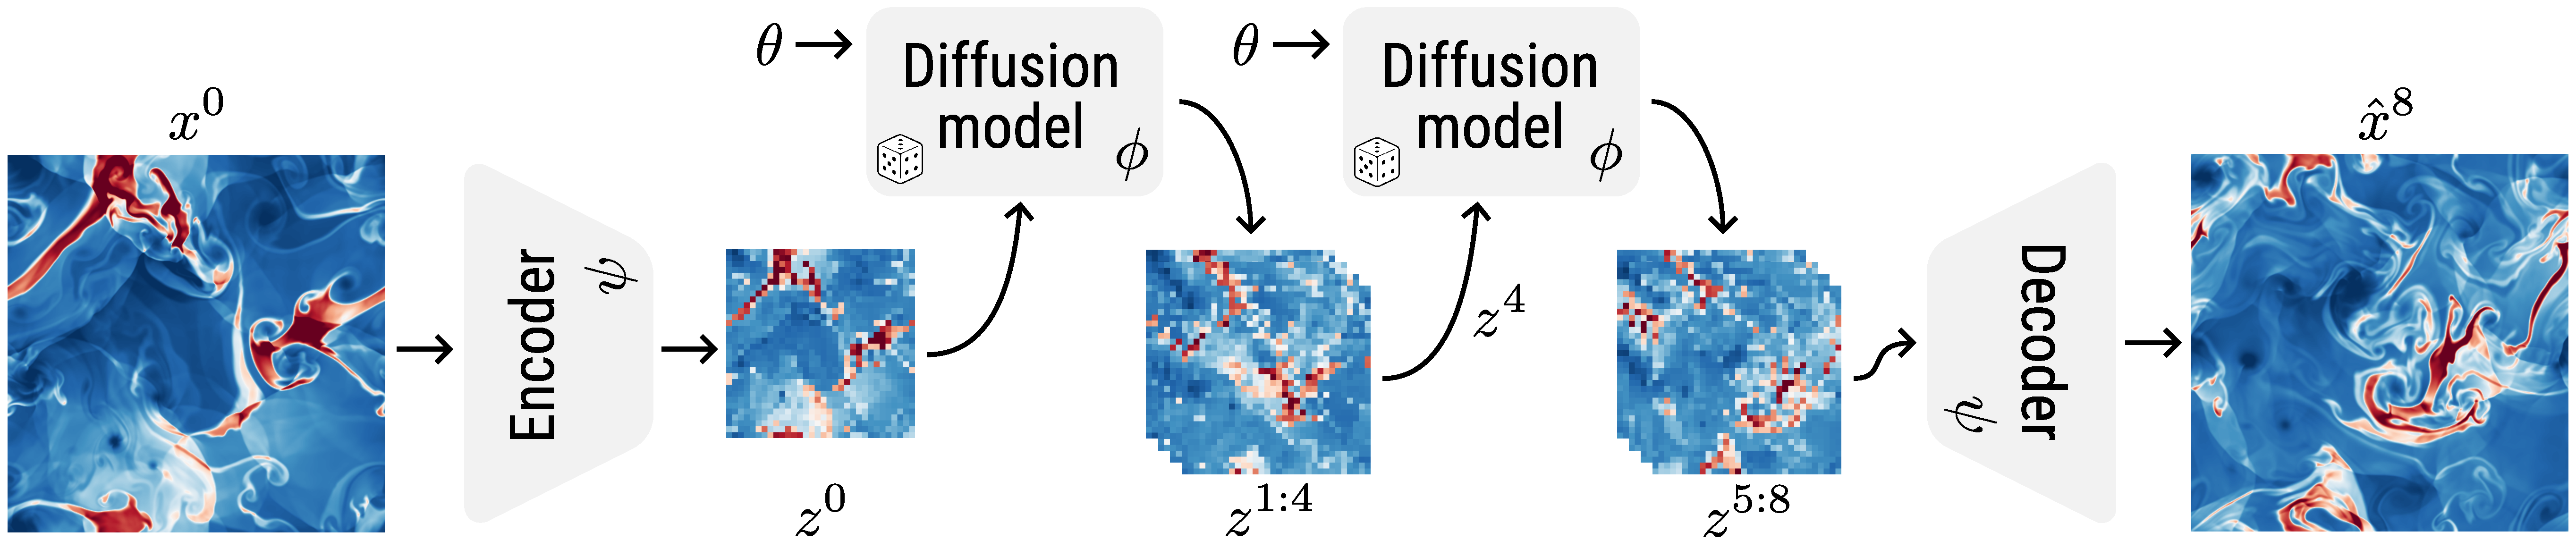
\includegraphics[width=0.95\textwidth]{./chapters/lola/figures/latent_emulation.pdf}
    \caption{Illustration of the latent-space emulation process. At each step of the autoregressive rollout, the diffusion model generates the next $n = 4$ latent states $z^{i+1:i+n}$ given the current state $z^i$ and the simulation parameters $\theta$. After rollout, the generated latent states are decoded to pixel space.}
    \label{fig:latent-emulation}
\end{figure}

\subsection{Datasets}

To study the effects of extreme compression rates, the datasets we consider should be high-dimensional and contain large amounts of data. Intuitively, the effective size of the dataset decreases in latent space, making overfitting more likely at fixed model capacity. According to these criteria, we select three datasets from TheWell \cite{ohana2024well}. Additional details are provided in Appendix~\ref{app:details}.

\paragraph{Euler Multi-Quadrants} The Euler equations model the behavior of compressible non-viscous fluids. In this dataset, the initial state presents multiple discontinuities which result in interacting shock waves as the system evolves for 100 steps. The 2d state of the system is represented with three scalar fields (energy, density, pressure) and one vector field (momentum) discretized on a $512 \times 512$ grid, for a total of $C_\text{pixel} = 5$ channels. Each simulation has either periodic or open boundary conditions and a different heat capacity $\gamma$, which constitutes their parameters $\theta$. We set a time stride $\Delta = 4$ between consecutive states $x^i$ and $x^{i+1}$, such that the simulation time $\tau = i \times \Delta$.

\paragraph{Rayleigh-Bénard (RB)} The Rayleigh-Bénard convection phenomenon occurs when a horizontal layer of fluid is heated from below and cooled from above. Over the 200 simulation steps, the temperature difference leads to the formation of convection currents where cooler fluid sinks and warmer fluid rises. The 2d state of the system is represented with two scalar fields (buoyancy, pressure) and one vector field (velocity) discretized on a $512 \times 128$ grid, for a total of $C_\text{pixel} = 4$ channels. Each simulation has different Rayleigh and Prandtl numbers as parameters $\theta$. We set a time stride $\Delta = 1$.

\paragraph{Turbulence Gravity Cooling (TGC)} The interstellar medium can be modeled as a turbulent fluid subject to gravity and radiative cooling. Starting from a homogeneous state, dense filaments form in the fluid, leading to the birth of stars. The 3d state of the system is represented with three scalar fields (density, pressure, temperature) and one vector field (velocity) discretized on a $64 \times 64 \times 64$ grid, for a total of $C_\text{pixel} = 6$ channels. Each simulation has different initial conditions function of their density, temperature, and metallicity. We set a time stride $\Delta = 1$.

\subsection{Autoencoders}

To isolate the effect of compression, we use a consistent autoencoder architecture and training setup across datasets and compression rates. We focus on compressing individual states $x^i$ into latent states $z^i = E_\psi(x^i)$, which are reconstructed as $\hat{x}^i = D_\psi(z^i)$.

\paragraph{Architecture} We adopt a convolution-based autoencoder architecture similar to the one used by \textcite{rombach2022highresolution}, which we adapt to perform well under high compression rates. Specifically, inspired by \textcite{chen2025deep}, we initialize the downsampling and upsampling layers near identity, which enables training deeper architectures with complex latent representations, while preserving reconstruction quality. For 2d datasets (Euler and RB), we set the spatial downsampling factor $r = 32$ for all autoencoders, meaning that a $32 \times 32$ patch in pixel space corresponds to one token in latent space. For 3d datasets (TGC), we set $r = 8$. The compression rate is then controlled solely by varying the number of channels per token in the latent representation. For instance, with the Euler dataset, an autoencoder with $C_\text{latent} = 64$ latent channels -- \texttt{f32c64} in the notations of \textcite{chen2025deep} -- transforms the input state with shape $512 \times 512 \times 5$ to a latent state with shape $16 \times 16 \times 64$, yielding a compression rate of $80$. This setup ensures that the architectural capacity remains similar for all autoencoders and allows for fair comparison across compression rates. Further details as well as a short ablation study are provided in Appendix \ref{app:details}.

\paragraph{Training} Latent diffusion models \cite{rombach2022highresolution} often rely on a Kullback-Leibler (KL) divergence penalty to encourage latents to follow a standard Gaussian distribution. However, this term is typically down-weighted by several orders of magnitude to prevent severe reconstruction degradation. As such, the KL penalty acts more as a weak regularization than a proper variational objective \cite{dieleman2025generative} and post-hoc standardization of latents is often necessary. We replace this KL penalty with a deterministic saturating function
\begin{equation}
    z \mapsto \frac{z}{\sqrt{1 + \nicefrac{z^2}{B^2}}}
\end{equation}
applied to the encoder's output. In our experiments, we choose the bound $B = 5$ to mimic the range of a standard Gaussian distribution. We find this approach simpler and more effective at structuring the latent space, without introducing a tradeoff between regularization and reconstruction quality. We additionally omit perceptual \cite{zhang2018unreasonable} and adversarial \cite{goodfellow2014generative, esser2021taming} loss terms, as they are designed for natural images where human perception is the primary target, unlike physics. The training objective thus simplifies to a reconstruction loss
\begin{equation}
    \arg\min_\psi \mathbb{E}_{p(x)} \left[ \ell(x, D_\psi(E_\psi(x))) \right] \, .
\end{equation}
The loss $\ell$ is typically a variation of $L_1$ or $L_2$ regression, which we discuss in Appendix \ref{app:details}. Finally, we find that preconditioned optimizers \cite{li2018preconditioned, gupta2018shampoo, vyas2025soap} greatly accelerate the training convergence of autoencoders compared to the widespread Adam \cite{kingma2015adam} optimizer (see Table \ref{tab:rb-ae-ablation}). We adopt the PSGD~\cite{li2018preconditioned} implementation in the \texttt{heavyball} \cite{nestler2022heavyball} library for its fewer number of tunable hyper-parameters and lower memory footprint than SOAP \cite{vyas2025soap}.

\subsection{Diffusion models}

\begin{figure}[b]
    \centering
    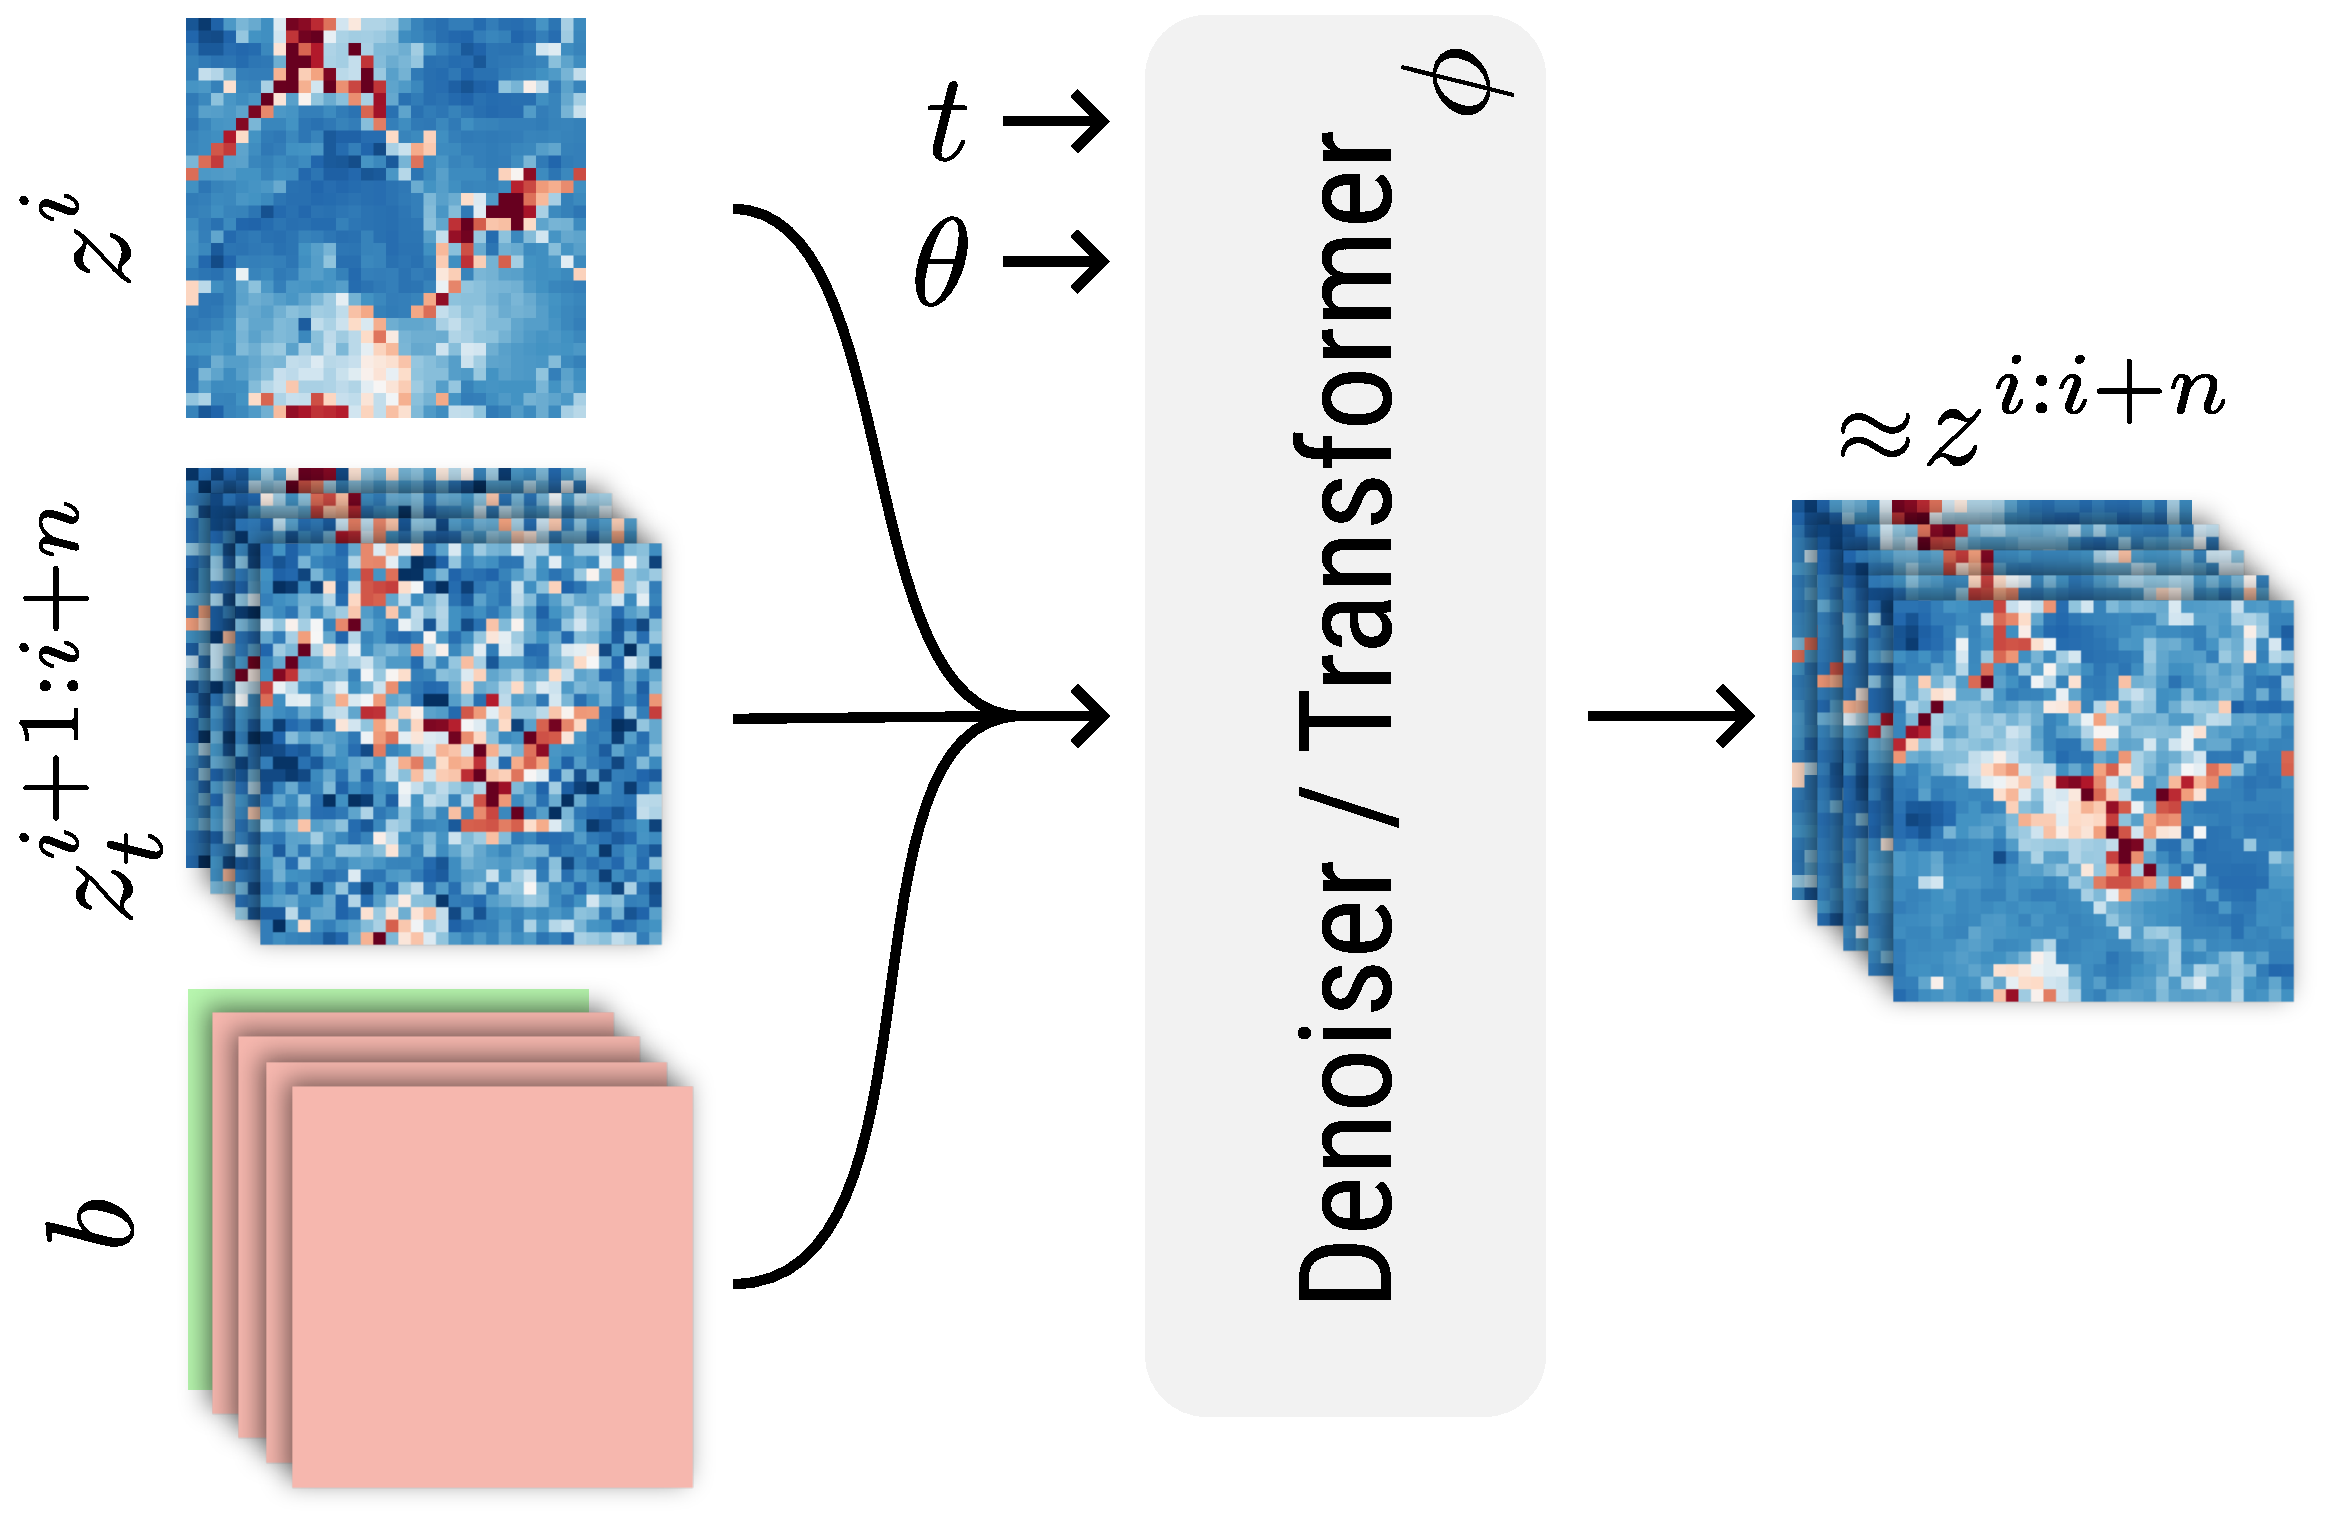
\includegraphics[width=0.5\textwidth]{./chapters/lola/figures/latent_denoiser.pdf}
    \caption{Illustration of the denoiser's inputs and outputs, while generating from $p(z^{i+1:i+n} \mid z^i, \theta)$. A binary mask $b$ is concatenated to the input to indicate which elements are noisy. The transformer blocks are modulated with respect to the parameters $\theta$ and the diffusion time $t$.}
    \label{fig:denoiser-io}
\end{figure}

We train diffusion models to predict the next $n$ latent states $z^{i+1:i+n}$ given the current state $z^i$ and simulation parameters $\theta$, that is to generate from $p(z^{i+1:i+n} \mid z^i, \theta)$. We parameterize our diffusion models with a denoiser $d_\phi(z_t^{i:i+n}, b, \theta, t)$ whose task is to denoise sequences of noisy states $z_t^{i} \sim p(z_t^{i} \mid z^{i}) = \mathcal{N}(z_t^{i} \mid \alpha_t \, z^{i}, \sigma_t^2 I)$ given the parameters $\theta$ of the simulation. Conditioning with respect to known elements in the sequence $z^{i:i+n}$ is tackled with a binary mask $b \in \{0, 1\}^{n+1}$ concatenated to the input, as in MCVD \cite{voleti2022mcvd}. For instance, $b = (1, 0, \dots, 0)$ indicates that the first element $z^i$ is known, while $b = (1, \dots, 1, 0)$ indicates that the first $n - 1$ elements $z^{i:i+n-1}$ are known. Known elements are provided to the denoiser without noise.

\paragraph{Architecture} Drawing inspiration from recent successes in latent image generation \cite{peebles2023scalable, karras2024analyzing, esser2024scaling, xie2025sana, chen2025deep}, we use a transformer-based architecture for the denoiser. We incorporate several architectural refinements shown to improve performance and stability, including query-key normalization \cite{henry2020querykey}, rotary positional embedding (RoPE) \cite{su2024roformer, heo2025rotary}, and value residual learning \cite{zhou2024value}. The transformer operates on the spatial and temporal axes of the input $z_t^{i:i+n}$, while the parameters $\theta$ and diffusion time $t$ modulate the transformer blocks. Thanks to the considerable ($r = 32$) spatial downsampling performed by the autoencoder, we are able to apply full spatio-temporal attention, avoiding the need for sparse attention patterns \cite{huang2019ccnet, ho2019axial, hassani2023neighborhood}. Finally, we fix the token embedding size (1024) and the number of transformer blocks (16) for all diffusion models. The only architectural variation stems from the number of input and output channels dictated by the corresponding autoencoder.

\paragraph{Training} As in Section \ref{sec:lola-diffusion}, diffusion models are trained via denoising score matching \cite{vincent2011connection, hyvarinen2005estimation}
\begin{equation}
    \arg\min_\phi \mathbb{E}_{p(\theta, z^{i:i+n}, z_t^{i:i+n}) p(b)} \Big[ \big\| d_\phi(\underbrace{z^{i:i+n} \odot b}_\text{clean} + \underbrace{z_t^{i:i+n} \odot (1 - b)}_\text{noisy}, b, \theta, t) - z^{i:i+n} \big\|_2^2 \Big]
\end{equation}
with the exception that the data does not come from the pixel-space distribution $p(\theta, x^{1:L})$ but from the latent-space distribution $p(\theta, z^{1:L})$ determined by the encoder $E_\psi$. Following \textcite{voleti2022mcvd}, we randomly sample the binary mask $b \sim p(b)$ during training to cover several conditioning tasks, including prediction with variable-length context $p(z^{i+c:i+n} \mid z^{i:i+c-1})$.

\paragraph{Sampling} After training, we sample from the learned distribution by solving Eq.~\eqref{eq:lola-reverse-sde} with $\eta = 0$, which corresponds to the probability flow ODE \cite{song2021scorebased}. To this end, we implement a 3rd order Adams-Bashforth multi-step integration method, as proposed by \textcite{zhang2023fast}. Intuitively, this method leverages information from previous integration steps to improve accuracy. We find this approach highly effective, producing high-quality samples with significantly fewer neural function evaluations (NFEs) than other widespread samplers~\cite{song2021denoising, karras2022elucidating}.

\subsection{Neural solvers}

We train neural solvers to perform the same task as diffusion models. Unlike the latter, however, solvers do not generate from $p(z^{i+1:i+n} \mid z^i, \theta)$, but produce a point estimate $f_\phi(z_i, \theta) \approx \mathbb{E}\big[ z^{i+1:i+n} \mid z_i, \theta \big]$ instead. We also train a pixel-space neural solver, for which $z^i = x^i$, as baseline.

\paragraph{Architecture} For latent-space neural solvers, we use the same transformer-based architecture as for diffusion models. The only notable difference is that transformer blocks are only modulated with respect to the simulation parameters $\theta$. For the pixel-space neural solver, we keep the same architecture, but group the pixels into $16 \times 16$ patches, as in vision transformers \cite{dosovitskiy2021image}. We also double the token embedding size (2048) such that the pixel-space neural solver has roughly two times more trainable parameters than an autoencoder and latent-space emulator combined.

\paragraph{Training} Neural solvers are trained via mean regression
\begin{equation}
    \arg\min_\phi \mathbb{E}_{p(\theta, z^{i:i+n}) p(b)} \left[ \big\| f_\phi(z^{i:i+n} \odot b, b, \theta) - z^{i:i+n} \big\|_2^2 \right] \, .
\end{equation}
Apart from the training objective, the training configuration (optimizer, learning rate schedule, batch size, epochs, masking, ...) for neural solvers is strictly the same as for diffusion models.

\subsection{Evaluation metrics}

We consider several metrics for evaluation, each serving a different purpose. We report these metrics either at a lead time $\tau = i \times \Delta$ or averaged over a lead time horizon $a\!:\!b$. If the states $x^i$ present several fields, the metric is first computed on each field separately, then averaged.

\paragraph{Variance-normalized RMSE} The root mean squared error (RMSE) and its normalized variants are widespread metrics to quantify the point-wise accuracy of an emulation \cite{fortin2014why, mccabe2023stability, ohana2024well}. Following \textcite{ohana2024well}, we pick the variance-normalized RMSE (VRMSE) over the more common normalized RMSE (NRMSE), as the latter down-weights errors in non-negative fields such as pressure and density. Formally, for two spatial fields $u$ and $v$, the VRMSE is defined as
\begin{equation} \label{eq:lola-vrmse}
    \operatorname{VRMSE}(u, v) = \sqrt{\frac{\left\langle (u - v)^2 \right\rangle}{\left\langle (u - \langle u \rangle)^2 \right\rangle + \epsilon}}
\end{equation}
where $\langle \cdot \rangle$ denotes the spatial mean operator and $\epsilon = \num{e-6}$ is a numerical stability term.

\paragraph{Power spectrum RMSE} For chaotic systems such as turbulent fluids, it is typically intractable to achieve accurate long-term emulation as very small errors can lead to entirely different trajectories later on. In this case, instead of reproducing the exact trajectory, emulators should generate diverse trajectories that remain statistically plausible. Intuitively, even though structures are wrongly located, the types of patterns and their distribution should stay similar \cite{dryden1943review}. Following \textcite{ohana2024well}, we assess statistical plausibility by comparing the power spectra of the ground-truth and emulated trajectories. For two spatial fields $u$ and $v$, we compute the isotropic power spectra $p_u$ and $p_v$ and split them into three frequency bands (low, mid and high) evenly distributed in log-space. We report the RMSE of the relative power spectra $\nicefrac{p_v}{p_u}$ over each band.

\paragraph{Spread-skill ratio} In earth sciences \cite{fortin2014why, price2025probabilistic}, the skill of an ensemble of $K$ particles is defined as the RMSE of the ensemble mean. The spread is defined as the ensemble standard deviation. Under these definitions and the assumption of a perfect forecast where ensemble particles are exchangeable, \textcite{fortin2014why} show that
\begin{equation}
    \operatorname{Skill} \approx \sqrt{\nicefrac{K+1}{K}} \, \operatorname{Spread} \, .
\end{equation}
This motivates the use of the (corrected) spread-skill ratio as a metric. Intuitively, if the ratio is smaller than one, the ensemble is biased or under-dispersed. If the ratio is larger than one, the ensemble is over-dispersed. It should be noted, however, that a spread-skill ratio of 1 is a necessary but insufficient condition for a perfect forecast.

\section{Results} \label{sec:lola-results}

We start with the evaluation of the autoencoders. For all datasets, we train three autoencoders with respectively 64, 16, and 4 latent channels. These correspond to compression rates of 80, 320 and 1280 for the Euler dataset, 64, 256, and 1024 for the RB dataset, and 48, 192, 768 for the TGC dataset, respectively. In the following, we refer to models by their compression rate. Additional experimental details are provided in Section \ref{sec:lola-methodology} and Appendix \ref{app:details}.

For each autoencoder, we evaluate the reconstruction $\hat{x}^i = D_\psi(E_\psi(x^i))$ of all states $x^i$ in 64 test trajectories $x^{0:L}$. As expected, when the compression rate increases, the reconstruction quality degrades, as reported in Figure \ref{fig:ae-vrmse}. For the Euler dataset, the reconstruction error grows with the lead time due to wavefront interactions and rising high-frequency content. For the RB dataset, the reconstruction error peaks mid-simulation during the transition from low to high-turbulence regime. Similar trends can be observed for the power spectrum RMSE in Tables \ref{tab:euler-power-rmse}, \ref{tab:rb-power-rmse} and \ref{tab:tgc-power-rmse}, where the high-frequency band is most affected by compression. These results so far align with what practitioners intuitively expect from lossy compression.

\begin{figure}[!h]
    \centering
    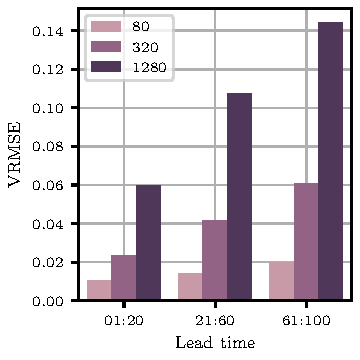
\includegraphics[width=0.32\textwidth]{./chapters/lola/figures/euler_ae_mean_absolute.pdf}
    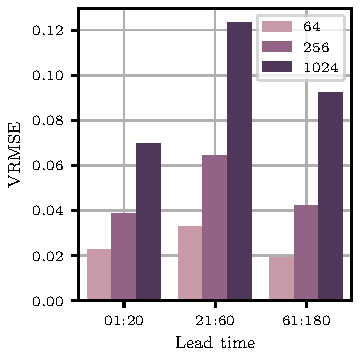
\includegraphics[width=0.32\textwidth]{./chapters/lola/figures/rb_ae_mean_absolute.pdf}
    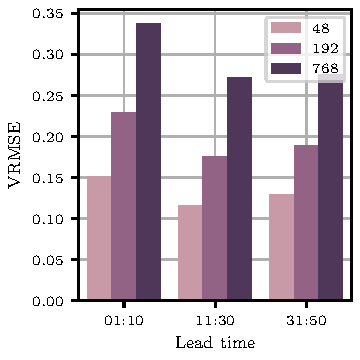
\includegraphics[width=0.32\textwidth]{./chapters/lola/figures/tgc_ae_mean_absolute.pdf}
    \caption{Average VRMSE of the autoencoder reconstruction at different compression rates and lead time horizons for the Euler (left), RB (center) and TGC (right) datasets. The compression rate has a clear impact on reconstruction quality.}
    \label{fig:ae-vrmse}
\end{figure}

We now turn to the evaluation of the emulators. For each autoencoder, we train two latent-space emulators: a diffusion model and a neural solver. Starting from the initial state $z^0 = E_\psi(x^0)$ and simulation parameters $\theta$ of 64 test trajectories $x^{0:L}$, each emulator produces 16 distinct autoregressive rollouts $z^{1:L}$, which are then decoded to the pixel space as $\hat{x}^i = D_\psi(z^i)$. Note that for neural solvers, all 16 rollouts are identical. We compute the metrics of each prediction $\hat{x}^i$ against the ground-truth state $x^i$.

As expected from imperfect emulators, the emulation error grows with the lead time, as shown in Figures \ref{fig:euler-mosaic} and \ref{fig:all-mosaic}. However, the point-wise error of diffusion models, as measured by the VRMSE, does not grow (Euler, TGC) and sometimes decreases (RB) with higher compression rates. Even at extreme ($>1000$) compression rates, latent-space emulators outperform the baseline pixel-space neural solver, despite the latter benefiting from more parameters and training compute. Similar observations can be made with the power spectrum RMSE over low and mid-frequency bands. High-frequency content, however, appears limited by the autoencoder's reconstruction capabilities. We confirm this hypothesis by recomputing the metrics relative to the autoencoded state $D_\psi(E_\psi(x^i))$, which we report in Figure~\ref{fig:all-mosaic-relative}. This time, the power spectrum RMSE of the diffusion models is low for mid and high-frequency bands. These findings support a puzzling narrative: emulation accuracy exhibits strong resilience to latent-space compression, starkly contrasting with the clear degradation in reconstruction quality.

\begin{figure}[!b]
    \vspace{-0.5em}
    \centering
    \includegraphics[width=\textwidth]{./chapters/lola/compressed/examples/example_1.pdf}
    \caption{Examples of latent-space emulation for the Euler (left) and Rayleigh-Bénard (right) datasets. Even for large compression rates ($\div$), latent-space emulators are able to reproduce the dynamics surprisingly faithfully, despite significant reconstruction artifacts. For Euler, wavefronts are accurately propagated until the end of the simulation, while vortices are well located, but distorted. For Rayleigh-Bénard, diffusion-based emulators produce plumes that grow at the correct pace but diverge from the ground-truth. Similar observations can be made in Figures \ref{fig:viz-euler-1} to \ref{fig:viz-tgc-4}.}
    \label{fig:viz-0}
\end{figure}

\begin{figure}[!b]
    \vspace{-0.5em}
    \centering
    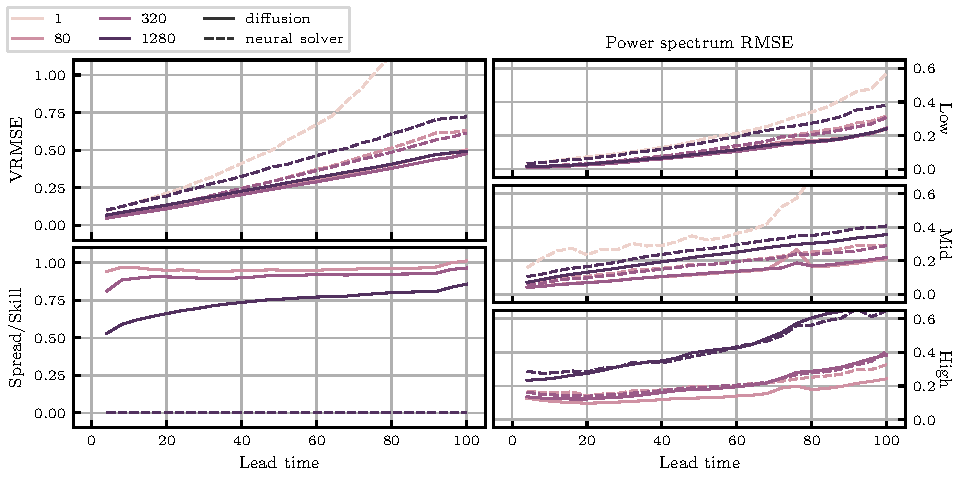
\includegraphics[width=\textwidth]{./chapters/lola/figures/euler_mosaic_mean_absolute.pdf}
    \caption{Average evaluation metrics of latent-space emulation for the Euler dataset. As expected from imperfect emulators, the emulation error grows with the lead time. However, the compression rate has little to no impact on diffusion-based emulation accuracy, beside high-frequency content. The spread-skill ratio \cite{fortin2014why, price2025probabilistic} drops slightly with the compression rate, which could be a sign of overfitting. Diffusion-based emulators are consistently more accurate than neural solvers.}
    \label{fig:euler-mosaic}
    \vspace{-0.5em}
\end{figure}

\begin{wraptable}{r}{0.4\textwidth}
    \centering
    \caption{Inference time per state for the Euler dataset, including generation and decoding.}
    \small
    \begin{tabular}{ccc}
        \toprule
        Method & Space & Time \\
        \midrule
        simulator & pixel & $\mathcal{O}(\qty{10}{\second})$ \\
        neural solver & pixel & \qty{56}{\milli\second} \\
        neural solver & latent & \qty{13}{\milli\second} \\
        diffusion & pixel & $\mathcal{O}(\qty{1}{\second})$ \\
        diffusion & latent & \qty{84}{\milli\second} \\
        \bottomrule
    \end{tabular}
    \label{tab:inference-time}
\end{wraptable}

Our experiments also provide a direct comparison between generative (diffusion) and deterministic (neural solver) approaches to emulation within a latent space. Figures \ref{fig:all-mosaic} and \ref{fig:all-mosaic-relative} indicate that diffusion-based emulators are consistently more accurate than their deterministic counterparts and generate trajectories that are statistically more plausible in terms of power spectrum. This can be observed qualitatively in Figure \ref{fig:viz-0} or Figures \ref{fig:viz-euler-1} to \ref{fig:viz-tgc-4} in Appendix \ref{app:emulation-results}. In addition, the spread-skill ratio of diffusion models is close to 1, suggesting that the ensemble of trajectories they produce are reasonably well calibrated in terms of uncertainty. However, the ratio slightly decreases with the compression rate. This phenomenon is partially explained by the smoothing effect of $L_2$-driven compression, and is therefore less severe in Figure \ref{fig:all-mosaic-relative}. Nonetheless, it remains present and could be a sign of overfitting due to the reduced amount of training data in latent space.

In terms of computational cost, although they remain slower than latent-space neural solvers, latent-space diffusion models are much faster than their pixel-space counterparts and competitive with pixel-space neural solvers (see Table \ref{tab:inference-time}). With our latent diffusion models, generating and decoding a full (100 simulation steps, 7 autoregressive steps) Euler trajectory takes 3 seconds on a single A100 GPU, compared to roughly 1 CPU-hour with the original numerical simulation \cite{mandli2016clawpack, ohana2024well}.

\begin{figure}[!b]
    \centering
    \includegraphics[width=\textwidth]{./chapters/lola/compressed/examples/example_2.pdf}
    \caption{Example of guided latent-space emulation for the RB (left) and TGC (right) datasets. The observations are the states downsampled by a factor 16 for RB and a stripe along the domain boundaries for TGC. Guidance is performed using the MMPS \cite{rozet2024learning} method. Thanks to the additional information in the observations, the emulation diverges less from the ground-truth.}
    \label{fig:rb-guidance}
\end{figure}

A final advantage of diffusion models lies in their capacity to incorporate additional information during sampling via guidance methods \cite{song2021scorebased, ho2022video, chung2023diffusion, rozet2023scorebased, rozet2024learning}. For example, if partial or noisy state observations are available, we can guide the emulation such that it remains consistent with these observations. We provide an illustrative example in Figure \ref{fig:rb-guidance} where guidance is performed with the MMPS \cite{rozet2024learning} method. Thanks to the additional information in the observations, the emulation diverges less from the ground-truth.

\section{Related work} \label{sec:lola-related-work}

Data-driven emulation of dynamical systems has become a prominent research area \cite{tompson2017accelerating, sanchez-gonzalez2020learning, pfaff2021learning, brandstetter2022message, stachenfeld2022learned, kovachki2023neural, lam2023learning, mccabe2024multiple, herde2024poseidon, morel2025disco} with diverse applications, including accelerating fluid simulations on uniform meshes using convolutional networks \cite{tompson2017accelerating, stachenfeld2022learned}, emulating various physics on non-uniform meshes with graph neural networks~\cite{sanchez-gonzalez2020learning, pfaff2021learning, brandstetter2022message, lam2023learning}, and solving partial differential equations with neural operators \cite{li2021fourier, raonic2023convolutional, hao2023gnot, mccabe2023stability, kovachki2023neural}. However, \textcite{mccabe2024multiple} and \textcite{herde2024poseidon} highlight the large data requirements of these methods and propose pre-training on multiple data-abundant physics before fine-tuning on data-scarce ones to improve data efficiency and generalization. Our experiments similarly suggest that large datasets are needed to train latent-space emulators.

A parallel line of work, related to reduced-order modeling \cite{benner2015survey}, focuses on learning low-dimensional representations of high-dimensional system states. Within this latent space, dynamics can be emulated more efficiently \cite{lusch2018deep, lui2019construction, wiewel2019latent, maulik2021reducedorder, han2022predicting, geneva2022transformers, chen2023crom, hemmasian2023reducedorder, li2025latent}. Various embedding approaches have been explored: convolutional autoencoders for uniform meshes \cite{wiewel2019latent, maulik2021reducedorder}, graph-based autoencoders for non-uniform meshes \cite{han2022predicting}, and implicit neural representations for discretization-free states \cite{chen2023crom, du2024conditional}. Koopman operator theory~\cite{koopman1931hamiltonian} has also been integrated into autoencoder training to promote linear latent dynamics \cite{yeung2019learning, geneva2022transformers}. Other approaches to enhance latent predictability include regularizing temporal derivatives~\cite{xie2024smooth}, jointly optimizing the decoder and latent emulator \cite{regazzoni2024learning}, and self-supervised prediction \cite{bardes2024revisiting}. While our work adopts this latent emulation paradigm, we do not impose structural biases on the latent space beside reconstruction quality.

A persistent challenge in neural emulation is ensuring temporal stability. Many models, while accurate for short-term prediction, exhibit long-term instabilities as errors accumulate, pushing the predictions out of the training data distribution \cite{mccabe2023stability}. Several strategies have been proposed to mitigate this issue: autoregressive unrolling during training \cite{lusch2018deep, geneva2020modeling, brandstetter2022message}, architectural modifications \cite{mccabe2023stability, raonic2023convolutional}, noise injection \cite{stachenfeld2022learned}, and post-processing \cite{lippe2023pderefiner, worrall2024spectral}. Generative models, particularly diffusion models, have recently emerged as a promising approach to address this problem \cite{lippe2023pderefiner, cachay2023dyffusion, kohl2024benchmarking, shysheya2024conditional, huang2024diffusionpde, price2025probabilistic} as they produce statistically plausible states, even when they diverge from the ground-truth solution.

While more accurate and stable, diffusion models are computationally expensive at inference. Drawing inspiration from latent space generation in computer vision \cite{rombach2022highresolution, peebles2023scalable, esser2024scaling, karras2024analyzing, xie2025sana, chen2025deep, polyak2024movie}, recent studies have applied latent diffusion models to emulate dynamical systems: \textcite{gao2023prediff} address short-term precipitation forecasting, \textcite{zhou2025text2pde} generate trajectories conditioned on text descriptions, \textcite{du2024conditional} generate trajectories within an implicit neural representation, and \textcite{li2025generative} combine a state-wise autoencoder with a spatio-temporal diffusion transformer \cite{peebles2023scalable} for autoregressive emulation, similar to our approach. These studies report favorable or competitive results against pixel-space and deterministic baselines, consistent with our observations.

\section{Discussion} \label{sec:lola-discussion}

Our results reveal key insights about latent physics emulation. First, diffusion-based emulation accuracy is surprisingly robust to latent-space compression, with performance remaining constant or even improving when autoencoder reconstruction quality significantly deteriorates. This observation is consistent with the latent generative modeling literature \cite{rombach2022highresolution, dieleman2025generative}, where compression serves a dual purpose: reducing dimensionality and filtering out perceptually irrelevant patterns that might distract from semantically meaningful information. Our experiments support this hypothesis as latent-space emulators outperform their pixel-space counterparts despite using fewer parameters and requiring less training compute. \textcite{yao2025reconstruction} similarly demonstrate that higher compression can sometimes improve generation quality despite degrading reconstruction. While our findings seem to violate the famous data processing inequality,\sidenote{\textit{The weakness of the Kolmogorov complexity theory is that it focuses on Shannon information and ignores computability.}\\[1ex] --- Ilya Sutskever (2023) \nocite{sutskever2023observation}} they are well aligned with the theory of \emph{usable} information \cite{xu2020theory}, where a learned representation can hold more $\mathcal{V}$-information from the point of view of a computationally constrained observer. Second, diffusion-based generative emulators consistently achieve higher ensemble accuracy than deterministic neural solvers while producing diverse, statistically plausible trajectories. This supports the idea that generative models mitigate distribution shift \cite{lippe2023pderefiner, cachay2023dyffusion, kohl2024benchmarking, shysheya2024conditional, huang2024diffusionpde, price2025probabilistic}. However, at the first prediction step, before distribution shift can take effect, diffusion models are already more accurate than deterministic neural solvers. This suggests an inherent modeling advantage, possibly lying in the iterative nature of diffusion sampling.

Despite the finite number of datasets, we believe that our findings are likely to generalize well across the broader spectrum of fluid dynamics. The Euler, RB and TGC datasets represent distinct fluid regimes that cover many key challenges in dynamical systems emulation: nonlinearities, multi-scale interactions, and complex spatio-temporal patterns. In addition, previous studies \cite{gao2023prediff, zhou2025text2pde, du2024conditional, li2025generative} come to similar conclusions for other fluid dynamics problems. However, we exercise caution about extending these conclusions beyond fluids. Systems governed by fundamentally different physics, such as chemical or quantum phenomena, may respond unpredictably to latent compression. Probing these boundaries represents an important direction for future research. Our empirical findings also prompt the need for theoretical explanations, which we leave to future work.

Apart from datasets, if compute resources were not a limiting factor, our study could be extended along several dimensions, although we anticipate that additional experiments would not fundamentally alter our conclusions. First, we could investigate techniques for improving the structure of the latent representation, such as incorporating Koopman-inspired losses \cite{yeung2019learning, geneva2022transformers}, regularizing temporal derivatives \cite{xie2024smooth}, or training shallow auxiliary decoders \cite{yao2025reconstruction, chen2025masked}. Second, we could probe the behavior of different embedding strategies under high compression, including spatio-temporal embeddings \cite{yu2023magvit, zhou2025text2pde, du2024conditional}, implicit neural representations \cite{chen2023crom, du2024conditional}, and masked autoencoders \cite{he2022masked, chen2025masked}. Third, we could add the capability to trade speed for accuracy, analogous to running numerical solvers at finer resolutions, by training an autoencoder with an adaptive latent dimensionality \cite{karkadaashok2018autoencoders, pham2022pcaae, bachmann2025flextok}. Fourth, we could study the effects of autoencoder and emulator capacity by scaling either up or down their number of trainable parameters. Each of these directions represents a substantial computational investment, particularly given the scale of our datasets and models, but would help establish best practices for latent-space emulation.

Nevertheless, our findings lead to clear recommendations for practitioners wishing to implement physics emulators. First, try latent-space approaches before pixel-space emulation. The former offer reduced computational requirements, lower memory footprint, and comparable or better accuracy across a wide range of compression rates. Second, prefer diffusion-based emulators over deterministic neural solvers. Latent diffusion models provide more accurate, diverse and stable long-term trajectories, while narrowing the inference speed gap significantly.

Our experiments, however, reveal important considerations about dataset scale when training latent-space emulators. The decreasing spread-skill ratio observed at higher compression rates suggests potential overfitting. This makes intuitive sense: as compression increases, the effective size of the dataset in latent space decreases, making overfitting more likely at fixed model capacity. Benchmarking latent emulators on smaller (10-100 GB) datasets like those used by \textcite{kohl2024benchmarking} could therefore yield misleading results. In addition, because the latent space is designed to preserve pixel space content, observing overfitting in this compressed representation suggests that pixel-space models encounter similar issues that remain undetected. This points towards the need for large training datasets or mixtures of datasets used to pre-train emulators before fine-tuning on targeted physics, as advocated by \textcite{mccabe2024multiple} and \textcite{herde2024poseidon}.

\section*{Acknowledgments}

We thank Géraud Krawezik and the Scientific Computing Core at the Flatiron Institute, a division of the Simons Foundation, for the compute facilities and support. We gratefully acknowledge use of the research computing resources of the Empire AI Consortium, Inc., with support from the State of New York, the Simons Foundation, and the Secunda Family Foundation. Polymathic AI acknowledges funding from the Simons Foundation and Schmidt Sciences, LLC. François Rozet is a research fellow of the F.R.S.-FNRS (Belgium) and acknowledges its financial support.

\clearpage
\section*{References}

\printbibliography[heading=none]

\begin{subappendices}

\clearpage
\section{Spread / Skill}

The skill \cite{fortin2014why, price2025probabilistic} of an ensemble of $K$ particles $v_k$ is defined as the RMSE of the ensemble mean
\begin{equation}
    \operatorname{Skill} = \sqrt{\left\langle \left( u - \frac{1}{K} \sum_{k=1}^K v_k \right)^2 \right\rangle}
\end{equation}
where $\langle \cdot \rangle$ denotes the spatial mean operator. The spread is defined as the ensemble standard deviation
\begin{equation}
    \operatorname{Spread} = \sqrt{\left\langle \frac{1}{K - 1} \sum_{j=1}^K  \left( v_j - \frac{1}{K} \sum_{k=1}^K v_k \right)^2 \right\rangle} \, .
\end{equation}
Under these definitions and the assumption of a perfect forecast where ensemble particles are exchangeable, \textcite{fortin2014why} show that
\begin{equation}
    \operatorname{Skill} \approx \sqrt{\frac{K+1}{K}} \, \operatorname{Spread} \, .
\end{equation}
This motivates the use of the (corrected) spread-skill ratio as a metric. Intuitively, if the ratio is smaller than one, the ensemble is biased or under-dispersed. If the ratio is larger than one, the ensemble is over-dispersed. It should be noted however, that a spread-skill ratio of 1 is a necessary but not sufficient condition for a perfect forecast.

\clearpage
\section{Experiment details} \label{app:details}

\paragraph{Datasets} For all datasets, each field is standardized with respect to its mean and variance over the training set. For Euler, the non-negative scalar fields (energy, density, pressure) are transformed with $x \mapsto \log (x + 1)$ before standardization. For TGC, the non-negative scalar fields (density, pressure, temperature) are transformed with $x \mapsto \log (x + \num{e-6})$ before standardization. When the states are illustrated graphically, as in Figure~\ref{fig:latent-emulation}, we represent the density field for Euler, the buoyancy field for RB, and a slice of the temperature field for TGC.

\begin{table}[!h]
    \centering
    \caption{Details of the selected datasets. We refer the reader to \textcite{ohana2024well} for more information.}
    \footnotesize
    \begin{tabular}{lccc}
        \toprule
        & Euler Multi-Quadrants & Rayleigh-Bénard & Turbulence Gravity Cooling \\
        \midrule
        Software & Clawpack \cite{mandli2016clawpack} & Dedalus \cite{burns2020dedalus} & ASURA-FDPS \cite{hirashima20233dspatiotemporal} \\
        Size & \qty{5243}{\giga\byte} & \qty{367}{\giga\byte} & \qty{849}{\giga\byte} \\
        \multirow{2}{*}{Fields} & energy, density, & buoyancy, pressure, & density, pressure, \\
        & pressure, velocity & momentum & temperature, velocity \\[0.25em]
        Channels $C_\text{pixel}$ & 5 & 4 & 6 \\
        Resolution & $512 \times 512$ & $512 \times 128$ & $64 \times 64 \times 64$ \\
        Discretization & Uniform & Chebyshev & Uniform \\
        Trajectories & 10000 & 1750 & 2700 \\
        Time steps $L$ & 100 & 200 & 50 \\
        Stride $\Delta$ & 4 & 1 & 1 \\
        \multirow{2}{*}{$\theta$} & heat capacity $\gamma$, & Rayleigh number, & hydrogen density $\rho_0$, \\
        & boundary conditions & Prandtl number & temperature $T_0$, metallicity $Z$ \\
        \bottomrule
    \end{tabular}
    \label{tab:datasets-details}
\end{table}

\paragraph{Autoencoders} The encoder $E_\psi$ and decoder $D_\psi$ are convolutional networks with residual blocks \cite{he2016deep}, SiLU \cite{elfwing2018sigmoidweighted} activation functions and layer normalization \cite{ba2016layer}. The output of the encoder is transformed with a saturating function (see Section \ref{sec:lola-methodology}). We provide a schematic illustration of the autoencoder architecture in Figure \ref{fig:ae-diagram}. Following \textcite{mccabe2024multiple}, we use a field-weighted loss $\ell$, and choose the variance-normalized MSE (VMSE)
\begin{equation} \label{eq:lola-vmse}
    \operatorname{VMSE}(u, v) = \frac{\big\langle (u - v)^2 \big\rangle}{\big\langle (u - \langle u \rangle)^2 \big\rangle + \epsilon}
\end{equation}
averaged over fields, where $\epsilon = \num{e-2}$ mitigates training instabilities. We train the encoder and decoder jointly for $1024 \times 256$ steps of the PSGD \cite{li2018preconditioned} optimizer. To mitigate overfitting we use random spatial axes permutations, flips and rolls as data augmentation. Each autoencoder takes 1 (RB), 2 (Euler) or 4 (TGC) days to train on 8 H100 GPUs. Other hyperparameters are provided in Table \ref{tab:ae-details}.

\begin{table}[!h]
    \centering
    \caption{Hyperparameters for the autoencoders.}
    \footnotesize
    \begin{tabular}{lcc}
        \toprule
        & Euler \& RB & TGC \\
        \midrule
        Architecture & Conv & Conv \\
        Parameters & \num{3.1e8} & \num{7.2e8} \\
        Pixel shape & $C_\text{pixel} \times H \times W$ & $C_\text{pixel} \times H \times W \times Z$ \\
        Latent shape & $C_\text{latent} \times \frac{H}{32} \times \frac{W}{32}$ & $C_\text{latent} \times \frac{H}{8} \times \frac{W}{8} \times \frac{Z}{8}$ \\[0.25em]
        Residual blocks per level & (3, 3, 3, 3, 3, 3) & (3, 3, 3, 3) \\
        Channels per level & (64, 128, 256, 512, 768, 1024) & (64, 256, 512, 1024) \\
        Kernel size & $3 \times 3$ & $3 \times 3 \times 3$ \\
        Activation & SiLU & SiLU \\
        Normalization & LayerNorm & LayerNorm \\
        Dropout & 0.05 & 0.05 \\
        \midrule
        Loss & VMSE & VMSE \\
        Optimizer & PSGD & PSGD \\
        Learning rate & \num{e-5} & \num{e-5} \\
        Weight decay & 0.0 & 0.0 \\
        Scheduler & cosine & cosine \\
        Gradient norm clipping & 1.0 & 1.0 \\
        Batch size & 64 & 64 \\
        Steps per epoch & 256 & 256 \\
        Epochs & 1024 & 1024 \\
        GPUs & 8 & 8 \\
        \bottomrule
    \end{tabular}
    \label{tab:ae-details}
\end{table}

\begin{table}[!h]
    \centering
    \caption{Short ablation study on the autoencoder architecture and training configurations. We pick the Rayleigh-Bénard dataset and an architecture with 64 latent channels to perform this study. The two major modifications that we propose are (1) the initialization of the downsampling and upsampling layers near identity, inspired by \textcite{chen2025deep}, and (2) the use of a preconditioned optimizer, PSGD~\cite{li2018preconditioned}, instead of Adam \cite{kingma2015adam}. We report the mean absolute error (MAE) on the validation set during training. The combination of both proposed modifications leads to order(s) of magnitude faster convergence.}
    \small
    \begin{tabular}{clcccc}
        \toprule
        \multirow[c]{2}{*}{Optimizer} & \multirow[c]{2}{*}{Id. init} & \multicolumn{3}{c}{Epoch} & \multirow[c]{2}{*}{Time} \\
        \cmidrule(lr){3-5}
        & & 10 & 100 & 1000 \\
        \midrule
        Adam & w/o & 0.065 & 0.029 & 0.017 & \qty{19}{\hour} \\
        Adam & w/ & 0.039 & 0.023 & 0.014 & \qty{19}{\hour} \\
        PSGD & w/ & 0.023 & 0.015 & 0.011 & \qty{25}{\hour} \\
        \bottomrule
    \end{tabular}
    \label{tab:rb-ae-ablation}
\end{table}

\begin{figure}[!h]
    \centering
    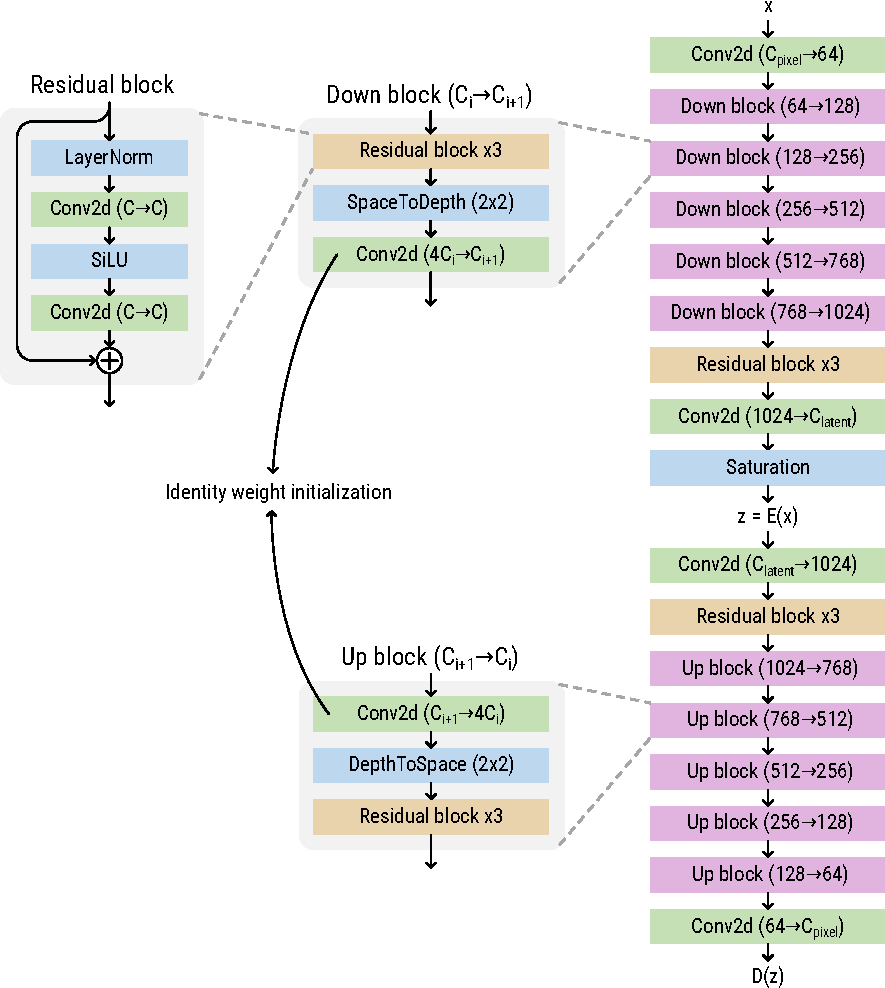
\includegraphics[width=\textwidth]{./chapters/lola/figures/ae_diagram.pdf}
    \caption{Schematic representation of the autoencoder architecture. Downsampling (resp. upsampling) is performed with a space-to-depth (resp. depth-to-space) operation followed (resp. preceded) with a convolution initialized near identity.}
    \label{fig:ae-diagram}
\end{figure}

\paragraph{Caching} The entire dataset is encoded with each trained autoencoder and the resulting latent trajectories are cached permanently on disk. The latter can then be used to train latent-space emulators, without needing to load and encode high-dimensional samples on the fly. Depending on hardware and data dimensionality, this approach can make a huge difference in I/O efficiency.

\clearpage
\paragraph{Emulators} The denoiser $d_\phi$ and neural solver $f_\phi$ are transformers with query-key normalization \cite{henry2020querykey}, rotary positional embedding (RoPE) \cite{su2024roformer, heo2025rotary}, and value residual learning \cite{zhou2024value}. The 16 blocks are modulated by the simulation parameters $\theta$ and the diffusion time $t$, as in diffusion transformers \cite{peebles2023scalable}. We train the emulator for $4096 \times 64$ steps of the Adam \cite{kingma2015adam} optimizer. Each latent-space emulator takes 2 (RB) or 5 (Euler, TGC) days to train on 8 H100 GPUs. Each pixel-space emulator takes 5 (RB) or 10 (Euler) days to train on 16 H100 GPUs. We do not train a pixel-space emulator for TGC. Other hyperparameters are provided in Table \ref{tab:emulator-details}

During training we randomly sample the binary mask $b$. The number of context elements $c$ follows a Poisson distribution $\operatorname{Pois}(\lambda = 2)$ truncated between $1$ and $n$. Hence, the masks $b$ take the form
\begin{equation}
    b = (\underbrace{1, \dots, 1}_{c}, 0, \dots, 0)
\end{equation}
implicitly defining a distribution $p(b)$.

\begin{table}[!h]
    \centering
    \caption{Hyperparameters for the emulators.}
    \footnotesize
    \begin{tabular}{lcc}
        \toprule
        & Latent-space & Pixel-space \\
        \midrule
        Architecture & Transformer & Transformer \\
        Parameters & \num{2.2e8} & \num{8.6e8} \\
        Input shape & $C_\text{latent} \times (n + 1) \times \frac{H}{32} \times \frac{W}{32}$ & $C_\text{pixel} \times (n + 1) \times H \times W$ \\
        Patch size & $1 \times 1 \times 1$ & $1 \times 16 \times 16$ \\
        Tokens & $(n + 1) \times \frac{H}{32} \times \frac{W}{32}$ & $(n + 1) \times \frac{H}{16} \times \frac{W}{16}$ \\[0.25em]
        Embedding size & 1024 & 2048 \\
        Blocks & 16 & 16 \\
        Positional embedding & Absolute + RoPE & Absolute + RoPE \\
        Activation & SiLU & SiLU \\
        Normalization & LayerNorm & LayerNorm \\
        Dropout & 0.05 & 0.05 \\
        \midrule
        Optimizer & Adam & Adam \\
        Learning rate & \num{e-4} & \num{e-4} \\
        Weight decay & 0.0 & 0.0 \\
        Scheduler & cosine & cosine \\
        Gradient norm clipping & 1.0 & 1.0 \\
        Batch size & 256 & 256 \\
        Steps per epoch & 64 & 64 \\
        Epochs & 4096 & 4096 \\
        GPUs & 8 & 16 \\
        \bottomrule
    \end{tabular}
    \label{tab:emulator-details}
\end{table}

\paragraph{Evaluation} For each dataset, we randomly select 64 trajectories $x^{0:L}$ with various parameters $\theta$ in the test set. For each latent-space emulator, we encode the initial state $z^0 = E_\psi(x^0)$ and produce 16 distinct autoregressive rollouts $z^{1:L}$. For the diffusion models, sampling is performed with 16 steps of the 3rd order Adams-Bashforth multi-step integration method \cite{zhang2023fast}. The metrics (VRMSE, power spectrum RMSE, spread-skill ratio) are then measured between the predicted states $\hat{x}^i = D_\psi(z^i)$ and the ground-truth states $x^i$ or the autoencoded states $D_\psi(E_\psi(x^i))$.

\clearpage
\section{Additional emulation results} \label{app:emulation-results}

\begin{figure}[!h]
    \centering
    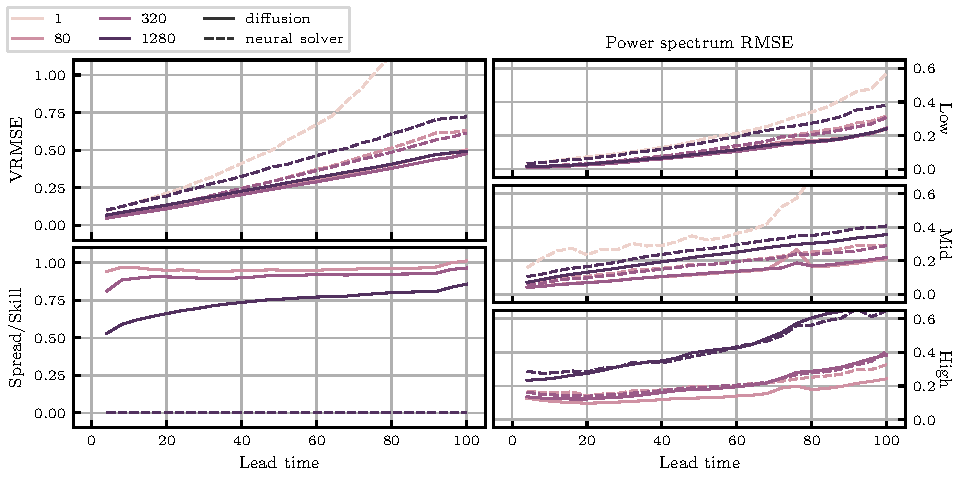
\includegraphics[width=\textwidth]{./chapters/lola/figures/euler_mosaic_mean_absolute.pdf}
    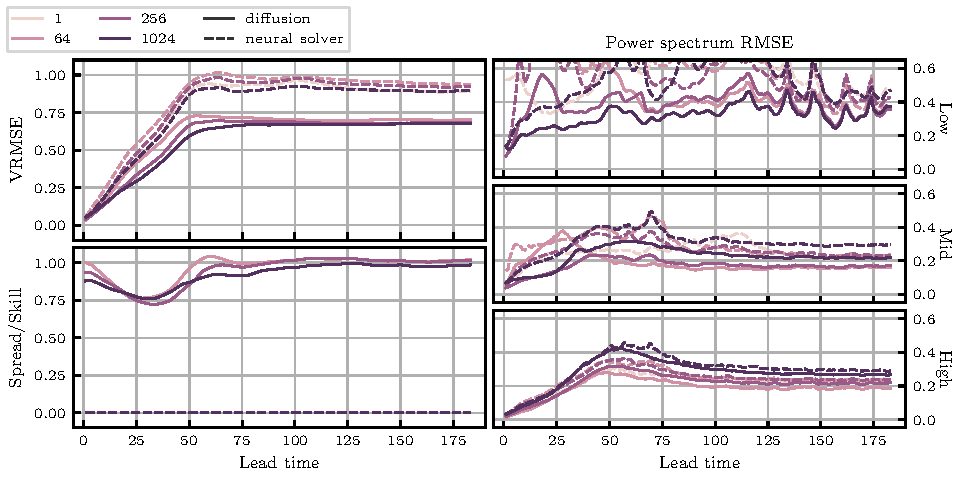
\includegraphics[width=\textwidth]{./chapters/lola/figures/rb_mosaic_mean_absolute.pdf}
    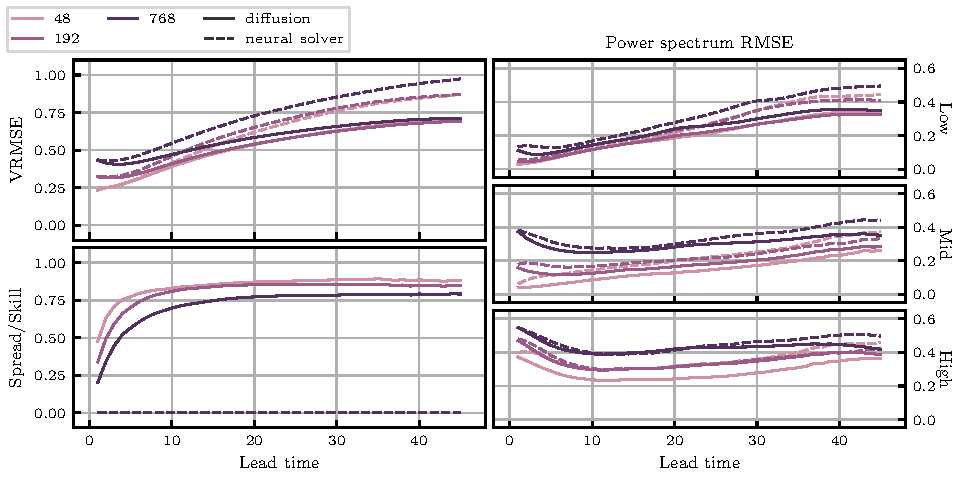
\includegraphics[width=\textwidth]{./chapters/lola/figures/tgc_mosaic_mean_absolute.pdf}
    \caption{Average evaluation metrics of latent-space emulation for the Euler (top), RB (center) and TGC (bottom) datasets. As expected from imperfect emulators, the emulation error grows with the lead time. However, increasing the compression rate does not degrade (Euler, TGC) and sometimes improves (RB) the accuracy of diffusion models. The spread-skill ratio \cite{fortin2014why, price2025probabilistic} drops slightly with the compression rate, which could be a sign of overfitting. Diffusion-based emulators are consistently more accurate than neural solvers.}
    \label{fig:all-mosaic}
\end{figure}

\begin{figure}[!h]
    \centering
    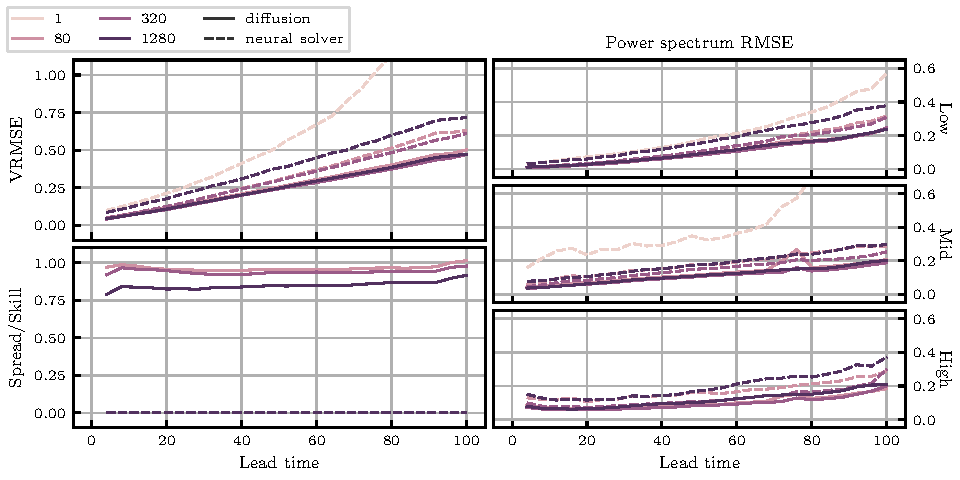
\includegraphics[width=\textwidth]{./chapters/lola/figures/euler_mosaic_mean_relative.pdf}
    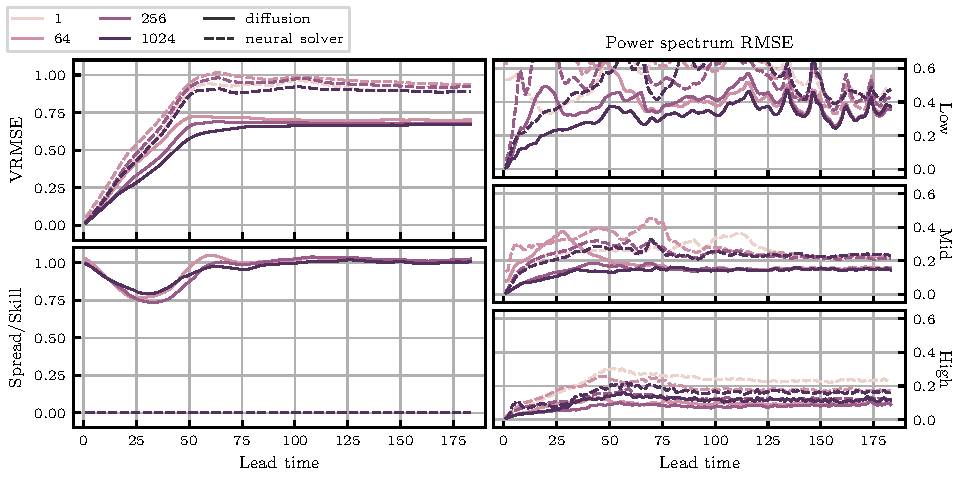
\includegraphics[width=\textwidth]{./chapters/lola/figures/rb_mosaic_mean_relative.pdf}
    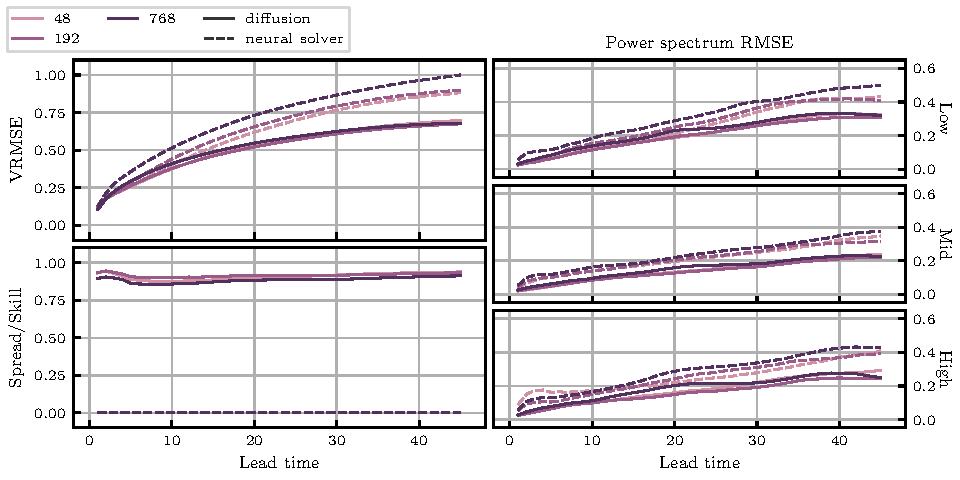
\includegraphics[width=\textwidth]{./chapters/lola/figures/tgc_mosaic_mean_relative.pdf}
    \caption{Average evaluation metrics of latent-space emulation relative to the autoencoded states $D_\psi(E_\psi(x^i))$ for the Euler (top), RB (center) and TGC (bottom) datasets. As expected from imperfect emulators, the emulation error grows with the lead time. However, increasing the compression rate does not degrade (Euler, TGC) and sometimes improves (RB) the accuracy of diffusion models. The spread-skill ratio \cite{fortin2014why, price2025probabilistic} drops slightly with the compression rate, which could be a sign of overfitting. Diffusion-based emulators are consistently more accurate than neural solvers.}
    \label{fig:all-mosaic-relative}
\end{figure}

\begin{table}[!h]
    \centering
    \caption{Average VRMSE of autoencoder reconstruction and latent-space emulation at different compression rates ($\div$) and lead time horizons for the Euler, RB and TGC datasets. Increasing the compression rate has a clear impact on reconstruction quality, but does not degrade significantly (Euler, TGC) and sometimes improves (RB) the accuracy of diffusion models.}
    \footnotesize
    \begin{tabular}{lrccc}
        \toprule
        \multirow[c]{2}{*}{Method} & \multicolumn{4}{c}{Euler} \\
        \cmidrule(lr){2-5}
         & $\div$ & 1:20 & 21:60 & 61:100 \\
        \midrule
        \multirow[c]{3}{*}{autoencoder}
        & 80 & 0.011 & 0.014 & 0.020 \\
        & 320 & 0.023 & 0.041 & 0.061 \\
        & 1280 & 0.060 & 0.107 & 0.144 \\
        \midrule
        \multirow[c]{3}{*}{diffusion}
        & 80 & 0.075 & 0.199 & 0.395 \\
        & 320 & 0.070 & 0.192 & 0.371 \\
        & 1280 & 0.093 & 0.217 & 0.400 \\
        \midrule
        \multirow[c]{4}{*}{neural solver}
        & 1 & 0.138 & 0.397 & 1.102 \\
        & 80 & 0.077 & 0.232 & 0.500 \\
        & 320 & 0.080 & 0.232 & 0.476 \\
        & 1280 & 0.137 & 0.314 & 0.592 \\
        \bottomrule
    \end{tabular}
    \hspace{1em}
    \begin{tabular}{lrccc}
        \toprule
        \multirow[c]{2}{*}{Method} & \multicolumn{4}{c}{RB} \\
        \cmidrule(lr){2-5}
         & $\div$ & 1:20 & 21:60 & 61:180 \\
        \midrule
        \multirow[c]{3}{*}{autoencoder}
        & 64   & 0.023 & 0.033 & 0.019 \\
        & 256  & 0.039 & 0.064 & 0.042 \\
        & 1024 & 0.070 & 0.124 & 0.092 \\
        \midrule
        \multirow[c]{3}{*}{diffusion}
        & 64   & 0.171 & 0.582 & 0.704 \\
        & 256  & 0.141 & 0.509 & 0.683 \\
        & 1024 & 0.146 & 0.457 & 0.670 \\
        \midrule
        \multirow[c]{4}{*}{neural solver}
        & 1    & 0.185 & 0.681 & 0.918 \\
        & 64   & 0.244 & 0.761 & 0.968 \\
        & 256  & 0.197 & 0.716 & 0.945 \\
        & 1024 & 0.195 & 0.665 & 0.903 \\
        \bottomrule
    \end{tabular}

    \vspace{1em}

    \begin{tabular}{lrccc}
        \toprule
        \multirow[c]{2}{*}{Method} & \multicolumn{4}{c}{TGC} \\
        \cmidrule(lr){2-5}
         & $\div$ & 1:10 & 11:20 & 21:50 \\
        \midrule
        \multirow[c]{3}{*}{autoencoder}
        & 48 & 0.151 & 0.116 & 0.129 \\
        & 192 & 0.229 & 0.175 & 0.189 \\
        & 768 & 0.338 & 0.272 & 0.276 \\
        \midrule
        \multirow[c]{3}{*}{diffusion}
        & 48 & 0.296 & 0.522 & 0.673 \\
        & 192 & 0.342 & 0.527 & 0.665 \\
        & 768 & 0.425 & 0.575 & 0.694 \\
        \midrule
        \multirow[c]{4}{*}{neural solver}
        & 48 & 0.302 & 0.599 & 0.826 \\
        & 192 & 0.361 & 0.632 & 0.835 \\
        & 768 & 0.462 & 0.710 & 0.920 \\
        \bottomrule
    \end{tabular}
    \label{tab:vrmse-vs-compression}
\end{table}

\begin{table}[!h]
    \centering
    \caption{Average VRMSE of latent-space emulation at different context lengths ($c$) and lead time horizons for the Euler, RB and TGC datasets. We can test different context lengths without retraining as our models were trained for different conditioning tasks (see Section \ref{sec:lola-methodology}). Perhaps surprisingly, context lengths does not have a significant impact on emulation accuracy.}
    \footnotesize
    \begin{tabular}{lcccc}
        \toprule
        \multirow[c]{2}{*}{Method} & \multicolumn{4}{c}{Euler} \\
        \cmidrule(lr){2-5}
         & $c$ & 1:20 & 21:60 & 61:100 \\
        \midrule
        \multirow[c]{3}{*}{diffusion}
        & 1 & 0.085 & 0.204 & 0.393 \\
        & 2 & 0.074 & 0.200 & 0.383 \\
        & 3 & 0.078 & 0.203 & 0.389 \\
        \midrule
        \multirow[c]{3}{*}{neural solver}
        & 1 & 0.108 & 0.266 & 0.526 \\
        & 2 & 0.092 & 0.253 & 0.513 \\
        & 3 & 0.094 & 0.260 & 0.529 \\
        \bottomrule
    \end{tabular}
    \hspace{1em}
    \begin{tabular}{lcccc}
        \toprule
        \multirow[c]{2}{*}{Method} & \multicolumn{4}{c}{RB} \\
        \cmidrule(lr){2-5}
         & $c$ & 1:20 & 21:60 & 61:180 \\
        \midrule
        \multirow[c]{3}{*}{diffusion}
        & 1 & 0.152 & 0.510 & 0.683 \\
        & 2 & 0.150 & 0.511 & 0.685 \\
        & 3 & 0.157 & 0.527 & 0.689 \\
        \midrule
        \multirow[c]{3}{*}{neural solver}
        & 1 & 0.208 & 0.705 & 0.932 \\
        & 2 & 0.209 & 0.708 & 0.943 \\
        & 3 & 0.220 & 0.728 & 0.940 \\
        \bottomrule
    \end{tabular}

    \vspace{1em}

    \begin{tabular}{lcccc}
        \toprule
        \multirow[c]{2}{*}{Method} & \multicolumn{4}{c}{TGC} \\
        \cmidrule(lr){2-5}
         & $c$ & 1:10 & 11:20 & 21:50 \\
        \midrule
        \multirow[c]{3}{*}{diffusion}
        & 1 & 0.362 & 0.550 & 0.681 \\
        & 2 & 0.351 & 0.535 & 0.669 \\
        & 3 & 0.350 & 0.539 & 0.683 \\
        \midrule
        \multirow[c]{3}{*}{neural solver}
        & 1 & 0.376 & 0.632 & 0.837 \\
        & 2 & 0.371 & 0.641 & 0.855 \\
        & 3 & 0.378 & 0.669 & 0.888 \\
        \bottomrule
    \end{tabular}
    \label{tab:vrmse-vs-context}
\end{table}

\begin{table}[h]
    \centering
    \caption{Average power spectrum RMSE of autoencoder reconstruction and latent-space emulation at different compression rates ($\div$) and lead time horizons for the Euler dataset. The high-frequency content of diffusion-based emulators is limited by the autoencoder's reconstruction capabilities.}
    \footnotesize
    \begin{tabular}{lrccccccccc}
        \toprule
        \multirow[c]{2}{*}{Method} & \multirow[c]{2}{*}{$\div$ \hspace{0.1em}} & \multicolumn{3}{c}{Low} & \multicolumn{3}{c}{Mid} & \multicolumn{3}{c}{High} \\
        \cmidrule(lr){3-5} \cmidrule(lr){6-8} \cmidrule(lr){9-11}
         & & 1:20 & 21:60 & 61:100 & 1:20 & 21:60 & 61:100 & 1:20 & 21:60 & 61:100 \\
        \midrule
        \multirow[c]{3}{*}{autoencoder}
        & 80 & 0.001 & 0.001 & 0.001 & 0.006 & 0.008 & 0.014 & 0.072 & 0.069 & 0.096 \\
        & 320 & 0.002 & 0.003 & 0.004 & 0.022 & 0.047 & 0.085 & 0.112 & 0.141 & 0.240 \\
        & 1280 & 0.009 & 0.017 & 0.025 & 0.074 & 0.167 & 0.264 & 0.240 & 0.355 & 0.577 \\
        \midrule
        \multirow[c]{3}{*}{diffusion}
        & 80 & 0.017 & 0.063 & 0.168 & 0.054 & 0.100 & 0.178 & 0.112 & 0.116 & 0.184 \\
        & 320 & 0.014 & 0.058 & 0.157 & 0.052 & 0.102 & 0.171 & 0.128 & 0.155 & 0.275 \\
        & 1280 & 0.019 & 0.065 & 0.163 & 0.096 & 0.187 & 0.300 & 0.246 & 0.349 & 0.569 \\
        \midrule
        \multirow[c]{4}{*}{neural solver}
        & 1 & 0.046 & 0.128 & 0.339 & 0.227 & 0.297 & 0.754 & 0.821 & 0.984 & 2.666 \\
        & 80 & 0.021 & 0.074 & 0.212 & 0.085 & 0.151 & 0.245 & 0.164 & 0.173 & 0.249 \\
        & 320 & 0.020 & 0.075 & 0.204 & 0.074 & 0.144 & 0.234 & 0.151 & 0.169 & 0.271 \\
        & 1280 & 0.045 & 0.116 & 0.274 & 0.131 & 0.227 & 0.349 & 0.283 & 0.345 & 0.545 \\
        \bottomrule
    \end{tabular}
    \label{tab:euler-power-rmse}
\end{table}

\begin{table}[h]
    \centering
    \caption{Average power spectrum RMSE of autoencoder reconstruction and latent-space emulation at different compression rates ($\div$) and lead time horizons for the Rayleigh-Bénard dataset. The high-frequency content of diffusion-based emulators is limited by the autoencoder's reconstruction capabilities.}
    \footnotesize
    \begin{tabular}{lrccccccccc}
        \toprule
        \multirow[c]{2}{*}{Method} & \multirow[c]{2}{*}{$\div$ \hspace{0.1em}} & \multicolumn{3}{c}{Low} & \multicolumn{3}{c}{Mid} & \multicolumn{3}{c}{High} \\
        \cmidrule(lr){3-5} \cmidrule(lr){6-8} \cmidrule(lr){9-11}
         & & 1:20 & 21:60 & 61:180 & 1:20 & 21:60 & 61:180 & 1:20 & 21:60 & 61:180 \\
        \midrule
        \multirow[c]{3}{*}{autoencoder}
        & 64   & 0.043 & 0.004 & 0.001 & 0.011 & 0.013 & 0.012 & 0.026 & 0.159 & 0.148 \\
        & 256  & 0.061 & 0.011 & 0.004 & 0.028 & 0.080 & 0.075 & 0.050 & 0.220 & 0.212 \\
        & 1024 & 0.121 & 0.033 & 0.018 & 0.063 & 0.186 & 0.197 & 0.076 & 0.294 & 0.294 \\
        \midrule
        \multirow[c]{3}{*}{diffusion}
        & 64   & 1.751 & 0.850 & 0.386 & 0.197 & 0.266 & 0.159 & 0.054 & 0.220 & 0.199 \\
        & 256  & 0.328 & 0.399 & 0.396 & 0.084 & 0.195 & 0.177 & 0.065 & 0.239 & 0.232 \\
        & 1024 & 0.193 & 0.292 & 0.344 & 0.095 & 0.243 & 0.240 & 0.083 & 0.314 & 0.297 \\
        \midrule
        \multirow[c]{4}{*}{neural solver}
        & 1    & 0.467 & 0.520 & 0.650 & 0.151 & 0.255 & 0.264 & 0.076 & 0.232 & 0.242 \\
        & 64   & 3.625 & 0.915 & 0.566 & 0.268 & 0.351 & 0.275 & 0.099 & 0.279 & 0.257 \\
        & 256  & 0.575 & 0.675 & 0.526 & 0.165 & 0.317 & 0.264 & 0.091 & 0.275 & 0.257 \\
        & 1024 & 0.285 & 0.496 & 0.560 & 0.152 & 0.338 & 0.321 & 0.090 & 0.320 & 0.326 \\
        \bottomrule
    \end{tabular}
    \label{tab:rb-power-rmse}
\end{table}

\begin{table}[h]
    \centering
    \caption{Average power spectrum RMSE of autoencoder reconstruction and latent-space emulation at different compression rates ($\div$) and lead time horizons for the TGC dataset. The high-frequency content of diffusion-based emulators is limited by the autoencoder's reconstruction capabilities.}
    \footnotesize
    \begin{tabular}{lrccccccccc}
        \toprule
        \multirow[c]{2}{*}{Method} & \multirow[c]{2}{*}{$\div$ \hspace{0.1em}} & \multicolumn{3}{c}{Low} & \multicolumn{3}{c}{Mid} & \multicolumn{3}{c}{High} \\
        \cmidrule(lr){3-5} \cmidrule(lr){6-8} \cmidrule(lr){9-11}
        & & 1:10 & 11:30 & 31:50 & 1:10 & 11:30 & 31:50 & 1:10 & 11:30 & 31:50 \\
        \midrule
        \multirow[c]{3}{*}{autoencoder}
        & 48 & 0.011 & 0.016 & 0.025 & 0.023 & 0.026 & 0.044 & 0.275 & 0.188 & 0.195 \\
        & 192 & 0.028 & 0.033 & 0.045 & 0.108 & 0.091 & 0.114 & 0.359 & 0.273 & 0.282 \\
        & 768 & 0.072 & 0.068 & 0.080 & 0.285 & 0.235 & 0.254 & 0.454 & 0.476 & 0.367 \\
        \midrule
        \multirow[c]{3}{*}{diffusion}
        & 48 & 0.064 & 0.185 & 0.319 & 0.058 & 0.128 & 0.220 & 0.296 & 0.247 & 0.331 \\
        & 192 & 0.069 & 0.191 & 0.311 & 0.128 & 0.164 & 0.252 & 0.369 & 0.316 & 0.384 \\
        & 768 & 0.107 & 0.294 & 0.425 & 0.289 & 0.305 & 0.360 & 0.456 & 0.419 & 0.444 \\
        \midrule
        \multirow[c]{3}{*}{neural solver}
        & 48 & 0.070 & 0.221 & 0.424 & 0.110 & 0.197 & 0.324 & 0.357 & 0.320 & 0.427 \\
        & 192 & 0.086 & 0.228 & 0.402 & 0.172 & 0.201 & 0.295 & 0.391 & 0.317 & 0.395 \\
        & 768 & 0.138 & 0.277 & 0.465 & 0.322 & 0.305 & 0.407 & 0.471 & 0.418 & 0.493 \\
        \bottomrule
    \end{tabular}
    \label{tab:tgc-power-rmse}
\end{table}

\begin{table}[h]
    \centering
    \caption{Average sliced earth mover's distance (SEMD) \cite{bonneel2015sliced, kolouri2019generalized} of the density field of autoencoder reconstruction and latent-space emulation at different compression rates ($\div$) and lead time horizons for the Euler dataset. The SEMD is small and is not significantly impacted by the compression rate, especially for diffusion models. For reference, the density fields of two consecutive states $x^i$ and $x^{i+1}$ have a typical SEMD of $0.0025$. \emph{Why this metric?} The Euler equations are sometimes used in aerodynamics to model flow around objects and one is typically interested in the global fluid displacement. The rationale for using this metric is that a small drift in the density field would not significantly affect the (S)EMD, while it could affect point-wise metrics heavily.}
    \footnotesize
    \begin{tabular}{lrccc}
        \toprule
        \multirow[c]{2}{*}{Method} & \multicolumn{4}{c}{EMD (density field)} \\
        \cmidrule(lr){2-5}
        & $\div$ & 1:20 & 21:60 & 61:100 \\
        \midrule
        \multirow[c]{3}{*}{autoencoder}
        & 80 & 0.0000 & 0.0000 & 0.0000 \\
        & 320 & 0.0001 & 0.0001 & 0.0001 \\
        & 1280 & 0.0002 & 0.0003 & 0.0005 \\
        \midrule
        \multirow[c]{3}{*}{diffusion}
        & 80 & 0.0004 & 0.0010 & 0.0023 \\
        & 320 & 0.0003 & 0.0009 & 0.0022 \\
        & 1280 & 0.0004 & 0.0010 & 0.0023 \\
        \midrule
        \multirow[c]{4}{*}{neural solver}
        & 1 & 0.0011 & 0.0031 & 0.0066 \\
        & 80 & 0.0005 & 0.0012 & 0.0028 \\
        & 320 & 0.0004 & 0.0012 & 0.0027 \\
        & 1280 & 0.0008 & 0.0020 & 0.0041 \\
        \bottomrule
    \end{tabular}
    \label{tab:emd-euler-vs-compression}
\end{table}

\begin{table}[h]
    \centering
    \caption{Average Wasserstein distance of the distribution of vertical velocity values of autoencoder reconstruction and latent-space emulation at different compression rates ($\div$) and lead time horizons for the RB dataset. The Wasserstein distance is smaller for diffusion models and decreases with the compression rate. For reference, the distributions of vertical velocity values of two consecutive states $x^i$ and $x^{i+1}$ have a typical Wasserstein distance of $0.004$. \emph{Why this metric?} One interesting quantity in buoyancy-driven convection is the growth speed of plumes in the fluid. The distribution of the (vertical) velocity values is a good summary statistic for tracking the growth of plumes.}
    \footnotesize
    \begin{tabular}{lrccc}
        \toprule
        \multirow[c]{2}{*}{Method} & \multicolumn{4}{c}{Wasserstein (vertical velocity field)} \\
        \cmidrule(lr){2-5}
         & $\div$ & 1:20 & 21:60 & 61:180 \\
        \midrule
        \multirow[c]{3}{*}{autoencoder}
        & 64   & 0.0000 & 0.0002 & 0.0002 \\
        & 256  & 0.0001 & 0.0007 & 0.0005 \\
        & 1024 & 0.0002 & 0.0020 & 0.0018 \\
        \midrule
        \multirow[c]{3}{*}{diffusion}
        & 64   & 0.0003 & 0.0104 & 0.0141 \\
        & 256  & 0.0003 & 0.0092 & 0.0141 \\
        & 1024 & 0.0004 & 0.0063 & 0.0139 \\
        \midrule
        \multirow[c]{4}{*}{neural solver}
        & 1    & 0.0003 & 0.0153 & 0.0247 \\
        & 64   & 0.0009 & 0.0272 & 0.0223 \\
        & 256  & 0.0007 & 0.0197 & 0.0187 \\
        & 1024 & 0.0007 & 0.0157 & 0.0206 \\
        \bottomrule
    \end{tabular}
    \label{tab:wasserstein-rb-vs-compression}
\end{table}

\begin{table}[h]
    \centering
    \caption{Average Wasserstein distance of the distribution of density values of autoencoder reconstruction and latent-space emulation at different compression rates ($\div$) and lead time horizons for the TGC dataset. The Wasserstein distance is smaller for diffusion models, but grows significantly with the lead time, even for the autoencoder reconstruction. For reference, the distributions of density values of two consecutive states $x^i$ and $x^{i+1}$ have a typical Wasserstein distance of $0.01$. \emph{Why this metric?} In the interstellar medium, gravity forms clusters of matter that eventually lead to the birth of stars. The kind of clusters (compact, diffuse, or anything in between) and their proportions is of interest for domain-scientists. The distribution of the density values is a good summary statistic for clustering dynamics.}
    \footnotesize
    \begin{tabular}{lrccc}
        \toprule
        \multirow[c]{2}{*}{Method} & \multicolumn{4}{c}{Wasserstein (density field)} \\
        \cmidrule(lr){2-5}
         & $\div$ & 1:10 & 11:30 & 31:50 \\
        \midrule
        \multirow[c]{3}{*}{autoencoder}
        & 48  & 0.0034 & 0.0048 & 0.0089 \\
        & 192 & 0.0082 & 0.0110 & 0.0183 \\
        & 768 & 0.0181 & 0.0236 & 0.0338 \\
        \midrule
        \multirow[c]{3}{*}{diffusion}
        & 48  & 0.0044 & 0.0138 & 0.0266 \\
        & 192 & 0.0089 & 0.0172 & 0.0310 \\
        & 768 & 0.0186 & 0.0274 & 0.0425 \\
        \midrule
        \multirow[c]{3}{*}{neural solver}
        & 48  & 0.0074 & 0.0253 & 0.0524 \\
        & 192 & 0.0091 & 0.0171 & 0.0329 \\
        & 768 & 0.0220 & 0.0296 & 0.0492 \\
        \bottomrule
    \end{tabular}
    \label{tab:wasserstein-tgc-vs-compression}
\end{table}

\begin{table}[h]
    \centering
    \caption{Average VRMSE results from various studies using TheWell \cite{ohana2024well} datasets. Even though our latent neural solvers (LNSs) and latent diffusion models (LDMs) outperform most published baselines, we emphasize that we do not position our models as state-of-the-art, due to the discrepancies in parameter count, training and evaluation. Notably, the U-Net and FNO baselines trained by \textcite{ohana2024well} are much smaller than other models, and their hyper-parameters were not tuned.}
    \footnotesize
    \begin{tabular}{lccccc}
        \toprule
        Source & Method & Dataset & Parameters & Lead time & VRMSE \\
        \midrule
        \textcite{ohana2024well} & FNO & Euler & \num{2e7} & 6:12 & 1.13 \\
        \textcite{ohana2024well} & U-Net & Euler & \num{2e7} & 6:12 & 1.02 \\
        Ours & ViT & Euler & \num{8.6e8} & 1:20 & 0.138 \\
        Ours & LNS $\div_{80}$ & Euler & \num{3.1e8} + \num{2.2e8} & 1:20 & 0.077 \\
        Ours & LDM $\div_{80}$ & Euler & \num{3.1e8} + \num{2.2e8} & 1:20 & 0.075 \\
        \midrule
        \textcite{ohana2024well} & FNO & RB & \num{2e7} & 6:12 & 10+ \\
        \textcite{ohana2024well} & U-Net & RB & \num{2e7} & 6:12 & 10+ \\
        \textcite{nguyen2025physix} & PhysiX & RB & \num{4.5e9} & 2:8 & 1.067 \\
        \textcite{wu2025tante} & TANTE & RB & \num{e8} & 1:16 & 0.609 \\
        \textcite{mukhopadhyay2025controllable} & ViT + CSM & RB & \num{e8} & 10 & 0.140 \\
        Ours & ViT & RB & \num{8.6e8} & 1:20 & 0.185 \\
        Ours & LNS $\div_{256}$ & RB & \num{3.1e8} + \num{2.2e8} & 1:20 & 0.197 \\
        Ours & LDM $\div_{256}$ & RB & \num{3.1e8} + \num{2.2e8} & 1:20 & 0.141 \\
        \midrule
        \textcite{ohana2024well} & FNO & TGC & \num{2e7} & 6:12 & 3.55 \\
        \textcite{ohana2024well} & U-Net & TGC & \num{2e7} & 6:12 & 7.14 \\
        \textcite{mukhopadhyay2025controllable} & ViT + CKM & TGC & \num{e8} & 10 & 0.527 \\
        Ours & LNS $\div_{48}$ & TGC & \num{7.2e8} + \num{2.2e8} & 1:10 & 0.302 \\
        Ours & LDM $\div_{48}$ & TGC & \num{7.2e8} + \num{2.2e8} & 1:10 & 0.296 \\
        \bottomrule
    \end{tabular}
    \label{tab:vrmse-baselines}
\end{table}

\begin{figure}[h]
    \centering
    \includegraphics[width=0.49\textwidth]{./chapters/lola/compressed/examples/example_3.pdf}
    \includegraphics[width=0.49\textwidth]{./chapters/lola/compressed/examples/example_4.pdf}
    \includegraphics[width=0.49\textwidth]{./chapters/lola/compressed/examples/example_5.pdf}
    \includegraphics[width=0.49\textwidth]{./chapters/lola/compressed/examples/example_6.pdf}
    \caption{Examples of emulation at different compression rates ($\div$) for the Euler dataset. In this simulation, the system has open boundary conditions.}
    \label{fig:viz-euler-1}
\end{figure}

\begin{figure}[h]
    \centering
    \includegraphics[width=0.49\textwidth]{./chapters/lola/compressed/examples/example_7.pdf}
    \includegraphics[width=0.49\textwidth]{./chapters/lola/compressed/examples/example_8.pdf}
    \includegraphics[width=0.49\textwidth]{./chapters/lola/compressed/examples/example_9.pdf}
    \includegraphics[width=0.49\textwidth]{./chapters/lola/compressed/examples/example_10.pdf}
    \caption{Examples of emulation at different compression rates ($\div$) for the Euler dataset. In this simulation, the system has periodic boundary conditions.}
    \label{fig:viz-euler-2}
\end{figure}

\begin{figure}[h]
    \centering
    \includegraphics[width=0.49\textwidth]{./chapters/lola/compressed/examples/example_11.pdf}
    \includegraphics[width=0.49\textwidth]{./chapters/lola/compressed/examples/example_12.pdf}
    \includegraphics[width=0.49\textwidth]{./chapters/lola/compressed/examples/example_13.pdf}
    \includegraphics[width=0.49\textwidth]{./chapters/lola/compressed/examples/example_14.pdf}
    \caption{Examples of emulation at different compression rates ($\div$) for the Euler dataset. In this simulation, the system has periodic boundary conditions.}
    \label{fig:viz-euler-3}
\end{figure}

\begin{figure}[h]
    \centering
    \includegraphics[width=0.49\textwidth]{./chapters/lola/compressed/examples/example_15.pdf}
    \includegraphics[width=0.49\textwidth]{./chapters/lola/compressed/examples/example_16.pdf}
    \includegraphics[width=0.49\textwidth]{./chapters/lola/compressed/examples/example_17.pdf}
    \includegraphics[width=0.49\textwidth]{./chapters/lola/compressed/examples/example_18.pdf}
    \caption{Examples of emulation at different compression rates ($\div$) for the Euler dataset. In this simulation, the system has periodic boundary conditions.}
    \label{fig:viz-euler-4}
\end{figure}

\begin{figure}[h]
    \centering
    \includegraphics[width=0.49\textwidth]{./chapters/lola/compressed/examples/example_19.pdf}
    \includegraphics[width=0.49\textwidth]{./chapters/lola/compressed/examples/example_20.pdf}
    \includegraphics[width=0.49\textwidth]{./chapters/lola/compressed/examples/example_21.pdf}
    \includegraphics[width=0.49\textwidth]{./chapters/lola/compressed/examples/example_22.pdf}
    \caption{Examples of emulation at different compression rates ($\div$) for the Rayleigh-Bénard dataset. In this simulation, the fluid is in a low-turbulence regime ($\mathrm{Ra} = \num{e6}$).}
    \label{fig:viz-rb-1}
\end{figure}

\begin{figure}[h]
    \centering
    \includegraphics[width=0.49\textwidth]{./chapters/lola/compressed/examples/example_23.pdf}
    \includegraphics[width=0.49\textwidth]{./chapters/lola/compressed/examples/example_24.pdf}
    \includegraphics[width=0.49\textwidth]{./chapters/lola/compressed/examples/example_25.pdf}
    \includegraphics[width=0.49\textwidth]{./chapters/lola/compressed/examples/example_26.pdf}
    \caption{Examples of emulation at different compression rates ($\div$) for the Rayleigh-Bénard dataset. In this simulation, the fluid is in a high-turbulence regime ($\mathrm{Ra} = \num{e8}$).}
    \label{fig:viz-rb-2}
\end{figure}

\begin{figure}[h]
    \centering
    \includegraphics[width=0.49\textwidth]{./chapters/lola/compressed/examples/example_27.pdf}
    \includegraphics[width=0.49\textwidth]{./chapters/lola/compressed/examples/example_28.pdf}
    \includegraphics[width=0.49\textwidth]{./chapters/lola/compressed/examples/example_29.pdf}
    \includegraphics[width=0.49\textwidth]{./chapters/lola/compressed/examples/example_30.pdf}
    \caption{Examples of emulation at different compression rates ($\div$) for the Rayleigh-Bénard dataset. In this simulation, the fluid is in a low-turbulence regime ($\mathrm{Ra} = \num{e6}$).}
    \label{fig:viz-rb-3}
\end{figure}

\begin{figure}[h]
    \centering
    \includegraphics[width=0.49\textwidth]{./chapters/lola/compressed/examples/example_31.pdf}
    \includegraphics[width=0.49\textwidth]{./chapters/lola/compressed/examples/example_32.pdf}
    \includegraphics[width=0.49\textwidth]{./chapters/lola/compressed/examples/example_33.pdf}
    \includegraphics[width=0.49\textwidth]{./chapters/lola/compressed/examples/example_34.pdf}
    \caption{Examples of emulation at different compression rates ($\div$) for the Rayleigh-Bénard dataset. In this simulation, the fluid is in a high-turbulence regime ($\mathrm{Ra} = \num{e8}$).}
    \label{fig:viz-rb-4}
\end{figure}

\begin{figure}[h]
    \centering
    \hspace{0.49\textwidth}
    \includegraphics[width=0.49\textwidth]{./chapters/lola/compressed/examples/example_36.pdf}
    \includegraphics[width=0.49\textwidth]{./chapters/lola/compressed/examples/example_37.pdf}
    \includegraphics[width=0.49\textwidth]{./chapters/lola/compressed/examples/example_38.pdf}
    \caption{Examples of emulation at different compression rates ($\div$) for the TGC dataset. In this simulation, the initial density is low and the initial temperature is low ($\rho_0 = 0.445$, $T_0 = 10.0$).}
    \label{fig:viz-tgc-1}
\end{figure}

\begin{figure}[h]
    \centering
    \hspace{0.49\textwidth}
    \includegraphics[width=0.49\textwidth]{./chapters/lola/compressed/examples/example_40.pdf}
    \includegraphics[width=0.49\textwidth]{./chapters/lola/compressed/examples/example_41.pdf}
    \includegraphics[width=0.49\textwidth]{./chapters/lola/compressed/examples/example_42.pdf}
    \caption{Examples of emulation at different compression rates ($\div$) for the TGC dataset. In this simulation, the initial density is medium and the initial temperature is high ($\rho_0 = 4.45$, $T_0 = 1000.0$).}
    \label{fig:viz-tgc-2}
\end{figure}

\begin{figure}[h]
    \centering
    \hspace{0.49\textwidth}
    \includegraphics[width=0.49\textwidth]{./chapters/lola/compressed/examples/example_44.pdf}
    \includegraphics[width=0.49\textwidth]{./chapters/lola/compressed/examples/example_45.pdf}
    \includegraphics[width=0.49\textwidth]{./chapters/lola/compressed/examples/example_46.pdf}
    \caption{Examples of emulation at different compression rates ($\div$) for the TGC dataset. In this simulation, the initial density is high and the initial temperature is low ($\rho_0 = 44.5$, $T_0 = 10.0$).}
    \label{fig:viz-tgc-3}
\end{figure}

\begin{figure}[h]
    \centering
    \hspace{0.49\textwidth}
    \includegraphics[width=0.49\textwidth]{./chapters/lola/compressed/examples/example_48.pdf}
    \includegraphics[width=0.49\textwidth]{./chapters/lola/compressed/examples/example_49.pdf}
    \includegraphics[width=0.49\textwidth]{./chapters/lola/compressed/examples/example_50.pdf}
    \caption{Examples of emulation at different compression rates ($\div$) for the TGC dataset. In this simulation, the initial density is high and the initial temperature is medium ($\rho_0 = 44.5$, $T_0 = 100.0$).}
    \label{fig:viz-tgc-4}
\end{figure}

\clearpage
\section{Latent space analysis} \label{app:latent-analysis}

In this section, we conduct a short analysis of the learned latent representations. We are notably interested in the separability of the latent representation with respect to different parameteres $\theta$.

For our first experiment, we select a random initial state $x^1$ from the test split of the Euler dataset. We compute the initial state $z^1 = E_\psi(x^1)$ for the $\div_{80}$ autoencoder. For each heat capacity $\gamma \in \{1.2, 1.3, 1.4, 1.5, 1.6\}$, we generate one latent trajectory $z^{1:L}$ with the diffusion-based emulator. Afterwards we compute the Euclidean distance $|| z^i_a - z^i_b ||_2$ for each pair $(\gamma_a, \gamma_b)$ of heat capacities. We report the results in Table \ref{tab:euler-theta-distance} and represent the trajectories in Figure \ref{fig:euler-theta-viz}. As expected, trajectories with similar heat capacity $\gamma$ are close to each others.

For our second experiment, we compute the latent representations $z^i = E_\psi(x^i) \in \mathbb{R}^{16 \times 4 \times 64}$ of the $\div_{64}$ autoencoder for randomly selected states $x^i$ of the Rayleigh-Bénard dataset. We then train a small multi-layer perceptron (MLP) to predict the simulation parameters $\theta$ (Rayleigh and Prandtl numbers) from the latent state's central token $z^i[8, 2] \in \mathbb{R}^{64}$. We extract the activations of the MLP's last layer and visualize them with t-SNE \cite{maaten2008visualizing} in Figure \ref{fig:rb-theta-tsne}. We observe that t-SNE \cite{maaten2008visualizing} continuously separates latent states with respect to their parameters $\theta$, indicating that our autoencoders learn to distinguish between different physics. We further validate this result by computing the pairwise Bures-Wasserstein distances \cite{peyre2019computational} between the distributions of central tokens $z^i[8, 2]$ for different Rayleigh and Prandtl numbers. The distances, reported in Tables \ref{tab:rb-rayleigh-bw} and \ref{tab:rb-prandtl-bw}, are anti-correlated with the similarity of simulation parameters $\theta$.

\begin{figure}[h]
    \centering
    \includegraphics[width=0.625\textwidth]{./chapters/lola/compressed/examples/example_51.pdf}
    \caption{Example of emulated trajectories with different heat capacities $\gamma \in \{1.2, 1.3, 1.4, 1.5, 1.6\}$ but starting at the same initial state $x^1$ for the Euler dataset. The energy field is visualized instead of the density field to emphasize the differences.}
    \label{fig:euler-theta-viz}
\end{figure}

\begin{table}[h]
    \centering
    \caption{Euclidean distance matrix between emulated trajectories with different heat capacities $\gamma \in \{1.2, 1.3, 1.4, 1.5, 1.6\}$ but starting at the same initial state $x^1$ for the Euler dataset.}
    \resizebox{\textwidth}{!}{%
    \begin{tabular}{c|ccccc}
    \toprule
    $\tau = 1$ & 1.2 & 1.3 & 1.4 & 1.5 & 1.6 \\
    \midrule
    1.2 & 0.00 & 26.61 & 32.45 & 38.46 & 46.28 \\
    1.3 & 26.61 & 0.00 & 14.72 & 22.09 & 32.33 \\
    1.4 & 32.45 & 14.72 & 0.00 & 15.26 & 25.62 \\
    1.5 & 38.46 & 22.09 & 15.26 & 0.00 & 18.52 \\
    1.6 & 46.28 & 32.33 & 25.62 & 18.52 & 0.00 \\
    \midrule
    $\tau = 60$ & 1.2 & 1.3 & 1.4 & 1.5 & 1.6 \\
    \midrule
    1.2 & 0.00 & 74.68 & 84.37 & 90.41 & 96.04 \\
    1.3 & 74.68 & 0.00 & 67.06 & 75.22 & 82.20 \\
    1.4 & 84.37 & 67.06 & 0.00 & 67.42 & 76.49 \\
    1.5 & 90.41 & 75.22 & 67.42 & 0.00 & 71.58 \\
    1.6 & 96.04 & 82.20 & 76.49 & 71.58 & 0.00 \\
    \bottomrule
    \end{tabular}
    \begin{tabular}{c|ccccc}
    \toprule
    $\tau = 20$ & 1.2 & 1.3 & 1.4 & 1.5 & 1.6 \\
    \midrule
    1.2 & 0.00 & 55.95 & 64.92 & 71.06 & 78.85 \\
    1.3 & 55.95 & 0.00 & 38.93 & 55.03 & 66.19 \\
    1.4 & 64.92 & 38.93 & 0.00 & 44.00 & 59.93 \\
    1.5 & 71.06 & 55.03 & 44.00 & 0.00 & 52.14 \\
    1.6 & 78.85 & 66.19 & 59.93 & 52.14 & 0.00 \\
    \midrule
    $\tau = 100$ & 1.2 & 1.3 & 1.4 & 1.5 & 1.6 \\
    \midrule
    1.2 & 0.00 & 74.71 & 82.09 & 90.16 & 94.79 \\
    1.3 & 74.71 & 0.00 & 66.72 & 74.16 & 81.68 \\
    1.4 & 82.09 & 66.72 & 0.00 & 67.51 & 74.72 \\
    1.5 & 90.16 & 74.16 & 67.51 & 0.00 & 69.75 \\
    1.6 & 94.79 & 81.68 & 74.72 & 69.75 & 0.00 \\
    \bottomrule
    \end{tabular}}
    \label{tab:euler-theta-distance}
\end{table}

\begin{figure}[h]
    \centering
    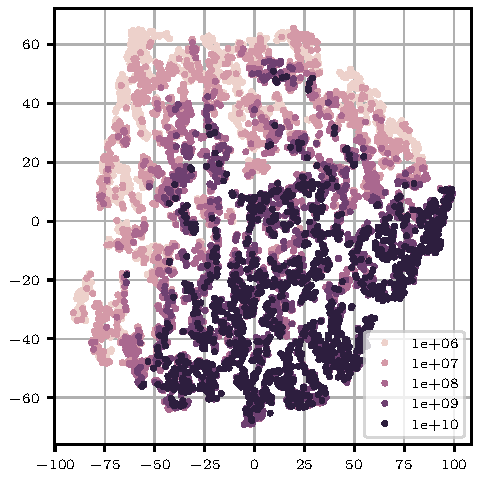
\includegraphics[width=0.49\textwidth]{./chapters/lola/figures/rb_tsne_rayleigh.pdf}
    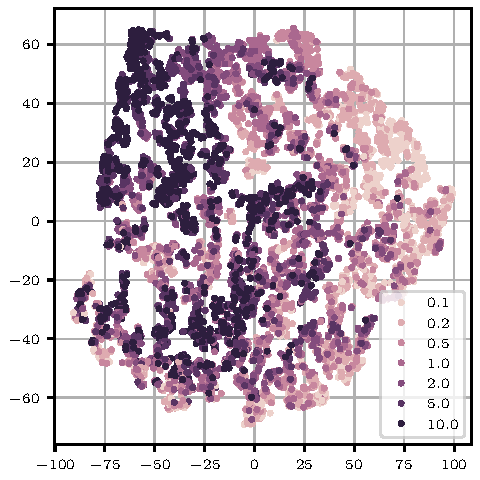
\includegraphics[width=0.49\textwidth]{./chapters/lola/figures/rb_tsne_prandtl.pdf}
    \caption{t-SNE \cite{maaten2008visualizing} visualization of the latent states $z^i = E_\psi(x^i)$. The projections are colored with respect to their Rayleigh (left) and Prandtl (right) numbers.}
    \label{fig:rb-theta-tsne}
\end{figure}

\begin{table}[h]
    \centering
    \caption{Bures-Wasserstein distance matrix between the distributions of latent states $z^i = E_\psi(x^i)$ with different Rayleigh numbers.}
    \footnotesize
    \begin{tabular}{l|ccccc}
    \toprule
    & \num{e6} & \num{e7} & \num{e8} & \num{e9} & \num{e10} \\
    \midrule
    \num{e6} & 0.000 & 1.045 & 1.708 & 2.279 & 2.489 \\
    \num{e7} & 1.045 & 0.000 & 0.965 & 1.537 & 1.794 \\
    \num{e8} & 1.708 & 0.965 & 0.000 & 0.915 & 1.180 \\
    \num{e9} & 2.279 & 1.537 & 0.915 & 0.000 & 0.714 \\
    \num{e10} & 2.489 & 1.794 & 1.180 & 0.714 & 0.000 \\
    \bottomrule
    \end{tabular}
    \label{tab:rb-rayleigh-bw}
\end{table}

\begin{table}[h]
    \centering
    \caption{Bures-Wasserstein distance matrix between the distributions of latent states $z^i = E_\psi(x^i)$ with different Prandtl numbers.}
    \footnotesize
    \begin{tabular}{l|ccccccc}
    \toprule
    & 0.1 & 0.2 & 0.5 & 1.0 & 2.0 & 5.0 & 10.0 \\
    \midrule
    0.1  & 0.000 & 1.367 & 2.042 & 2.631 & 3.244 & 3.884 & 4.210 \\
    0.2  & 1.367 & 0.000 & 1.269 & 1.839 & 2.381 & 3.007 & 3.331 \\
    0.5  & 2.042 & 1.269 & 0.000 & 0.986 & 1.479 & 2.093 & 2.398 \\
    1.0  & 2.631 & 1.839 & 0.986 & 0.000 & 0.930 & 1.472 & 1.766 \\
    2.0  & 3.244 & 2.381 & 1.479 & 0.930 & 0.000 & 0.988 & 1.251 \\
    5.0  & 3.884 & 3.007 & 2.093 & 1.472 & 0.988 & 0.000 & 0.711 \\
    10.0 & 4.210 & 3.331 & 2.398 & 1.766 & 1.251 & 0.711 & 0.000 \\
    \bottomrule
    \end{tabular}
    \label{tab:rb-prandtl-bw}
\end{table}

\end{subappendices}

\chapter[Latent Score-based Data Assimilation]{Latent Score-based\\Data Assimilation} \label{chap:appa}

\begin{quote}
    \textit{Imagine a system on a rotating sphere that is 8000 miles wide, consists of different materials, different gases that have different properties (one of the most important of which, water, exists in different concentrations), heated by a nuclear reactor 98 million miles away. Then, just to make life interesting, this sphere is oriented such that, as it revolves around the nuclear reactor, it is heated differently at different locations at different times of the year. Then, someone is asked to watch the mixture of gases, a fluid only 20 miles deep, that covers an area of 250 million square miles, and to predict the state of that fluid at one point on the sphere two days from now. This is the problem weather forecasters face.}

    \begin{flushright}
        --- Robert T. Ryan (1982) \nocite{ryan1982weather}
    \end{flushright}
\end{quote}

\vspace{2em}

\begin{addendum}{\Large\scshape Addendum}

This chapter appeared previously as

\begin{itemize}[leftmargin=1em]
    \item[] \fullcite{andry2025appa}.
\end{itemize}

Gérôme and Sacha implemented the methods, conducted the experiments, interpreted the results, and wrote most of the manuscript. François came up with the methods, supervised the codebase, and wrote the technical parts of the manuscript. Omer, Victor and Matthias contributed to the codebase and the visualization of the results. Elise provided valuable domain knowledge. Gilles supervised the project, suggested experiments, and participated in the writing.

For the version presented in this chapter, we have edited the structure and content of the manuscript to be consistent with the rest of this document. At the time of writing, the Appa project is still in progress and is not published within a peer-reviewed venue. Nevertheless, we wish to include this early version in this dissertation, as it is a logical continuation of our work.

\end{addendum}

\section*{Abstract}

While deep learning has been transformative for numerical weather prediction, the assimilation step preceding forecasting that estimates the current atmospheric state from observational data remains challenging. In this work, we introduce Appa, a score-based data assimilation model generating global atmospheric trajectories at \qty{0.25}{\degree} resolution and 1-hour intervals. Powered by a 565M latent diffusion model trained on ERA5, Appa can be conditioned on arbitrary observations to infer plausible trajectories, without retraining. Our probabilistic framework handles reanalysis, filtering, and forecasting as special cases. Results establish latent score-based data assimilation as a promising foundation for future global atmospheric modeling systems.

\section{Introduction} \label{sec:appa-introduction}

Data assimilation combines observational data with physical models to estimate atmospheric states. Formally, let $x^{1:L} = (x^1, x^2, \dots, x^L) \in \mathbb{R}^{L \times V \times C}$ denote a trajectory of $L$ atmospheric states, each represented as $C$ physical fields over a mesh of $V$ vertices. Let $p(x^1)$ be the initial state prior and $p(x^{i+1} \mid x^i)$ the transition dynamics. Observations $y^{1:L} \in \mathbb{R}^{M_1 + \dots + M_L}$ of the states $x^{1:L}$ follow an observation process $p(y^i \mid x^i)$, generally formulated as $y^i = \mathcal{H}^i(x^i) + \eta^i$, where the measurement functions $\mathcal{H}^i: \mathbb{R}^{V \times C} \mapsto \mathbb{R}^{M_i}$ can be non-linear and $\eta^i \in \mathbb{R}^{M_i}$ represents observational error that accounts for instrumental noise and systematic uncertainties. The goal of data assimilation is to infer plausible trajectories $x^{1:L}$ consistent with the observations $y^{1:L}$, that is, to estimate the trajectory posterior
\begin{equation} \label{eq:general-assim}
    p(x^{1:L} \mid y^{1:L}) \propto p(x^1) \prod_{i=1}^{L-1} p(x^{i+1} \mid x^i) \prod_{i=1}^{L} p(y^i \mid x^i) \, .
\end{equation}
While Eq.~\eqref{eq:general-assim} defines the general assimilation problem, assimilation tasks correspond to specific choices of states $x^i$ to infer and observations $y^i$ to take into account. In this work, we focus on three special cases:
\begin{align}
    \textbf{Reanalysis}  \quad & p(x^{1:L} \mid y^{1:L}) \, , \label{eq:reanalysis} \\
    \textbf{Filtering}   \quad & p(x^L \mid y^{1:L}) \, , \label{eq:filtering} \\
    \textbf{Forecasting} \quad & p(x^{K+1:L} \mid y^{1:K}) \, . \label{eq:forecast}
\end{align}
Reanalysis aims to reconstruct full trajectories from historical observations. The primary purpose of reanalysis is to create datasets of historical data for the land, atmosphere, and oceans. These datasets enable scientists to better monitor and understand the climate, conduct surveys, and develop new weather models. Filtering, in contrast, only infers the posterior distribution of the last/current state $x^L$. This step is crucial to initialize global weather models in numerical weather prediction. Forecasting, as its name suggests, extends beyond the observed segment, producing posterior distributions over future states. The forecasting problem is often decomposed into first estimating the current state $x^K$ from $y^{1:K}$, and then predicting its evolution.

Traditional assimilation methods like 4D-Var~\cite{lorenc1986analysis, ledimet1986variational, tremolet2006accounting, tremolet2007modelerror, fisher2011weakconstraint} or ensemble Kalman filters~\cite{evensen1994sequential, bishop2001adaptive, anderson2007adaptive, hunt2007efficient, evensen2009data} are effective but rely on linearization and differentiation of the transition dynamics, which is very expensive at a global scale. In addition, 4D-Var provides point estimates instead of a posterior distribution~\cite{carrassi2018data}. Recent data-driven approaches~\cite{cheng2023machine, huang2024diffda, xu2025fuxida, fablet2021joint, andrychowicz2023deep} integrate deep learning into assimilation, but suffer from limited resolution, lack of uncertainty quantification, and require retraining for new observation configurations.

\section{Appa} \label{sec:appa}

Appa combines score-based data assimilation~\cite{rozet2023scorebased, rozet2023scorebaseda, schmidt2025generative} with latent diffusion-based physics emulation~\cite{rozet2025lost}, scaled to the global atmospheric system at \qty{0.25}{\degree} resolution and 1-hour intervals. It consists of (1) a 340M encoder-decoder pair $(E_\psi, D_\psi)$ that compresses atmospheric states $x^i$ into $530\times$ smaller latent representations $z^i \sim \mathcal{N}(z^i \mid E_\psi(x^i), \sigma_z^2 I)$ and (2) a 225M diffusion transformer (DiT) \cite{peebles2023scalable} that generates windows $z^{i:i+W}$ of $W = 24$ consecutive latent states.

The encoder and decoder are trained to minimize the $L_2$ error between states $x^i$ and their reconstruction $\hat{x}^i = D_\psi(z^i)$. The DiT $d_\phi(z^{i:i+W}_t)$ is trained to estimate the denoising posterior mean $\mathbb{E}[z^{i:i+W} \mid z^{i:i+W}_t]$ for noisy latent states $z^{i:i+W}_t \sim \mathcal{N}(\alpha_t \, z^{i:i+W}, \sigma_t^2 I)$. Tweedie's formula~\cite{tweedie1947functions, efron2011tweedies, kim2021noise2score}
\begin{equation}
    \mathbb{E} \big[z^{i:i+W} \mid z^{i:i+W}_t\big] = \frac{z^{i:i+W}_t + \sigma^2_t \, \grad{z^{i:i+W}_t} \log p(z^{i:i+W}_t)}{\alpha_t}
\end{equation}
then gives access to the prior score $\grad{z^{i:i+W}_t} \log p(z^{i:i+W}_t)$ necessary to simulate the reverse diffusion process \cite{song2021scorebased}. As in the SDA~\cite{rozet2023scorebased, rozet2023scorebaseda} framework, the score over longer trajectories $z^{1:L}_t$ is approximated by composing the scores over windows $z^{i:i+W}_t$. Algorithm \ref{alg:appa-composing} generalizes SDA's composition algorithm by introducing a time stride $\Delta \geq 1$ between consecutive windows. Using a larger stride reduces the window overlap and, therefore, the number of network evaluations.

\begin{figure}[b]
\begin{minipage}[t]{0.49\textwidth}%
\vspace{-1em}
\begin{algorithm}[H]
    \caption{Training $d_\phi(z^{i:i+W}_t)$} \label{alg:appa-training}
    \begin{algorithmic}[1]
        \For{$n = 1$ to $N$}
            \State $x^{1:L} \sim p(x^{1:L})$
            \State $i \sim \mathcal{U}(\{1, \dots, L-W\})$
            \State $t \sim \mathcal{U}(0, 1) \, , \varepsilon \sim \mathcal{N}(0, I)$
            \For{$j = i$ to $i + W$}
                \State $z_j \gets E_\psi(x_j)$
            \EndFor{}
            \State $z^{i:i+W}_t \gets \alpha_t \, z^{i:i+W} + \sigma_t \, \varepsilon$
            \State $\displaystyle \ell \gets \big\| d_\phi(z^{i:i+W}_t) - z^{i:i+W} \big\|^2_2$
            \State $\phi \gets \Call{SGD}{\phi, \grad{\phi} \, \ell}$
        \EndFor{}
	\end{algorithmic}
\end{algorithm}
\end{minipage}%
\hfill%
\begin{minipage}[t]{0.49\textwidth}%
\vspace{-1em}
\begin{algorithm}[H]
    \caption{Composing $d_\phi(z^{i:i+W}_t)$} \label{alg:appa-composing}
    \begin{algorithmic}[1]
        \Function{$d_\phi(z^{1:L}_t)$}{}
            \State $a \gets \nicefrac{(W - \Delta)}{2}$
            \State $b \gets a + \Delta$
            \State $E_{1:a} \gets d_\phi(z^{1:1+W}_t)[:\!a]$
            \For{$n = 0$ to $\nicefrac{(L - W)}{\Delta} + 1$}
                \State $i \gets 1 + n \Delta$
                \State $E_{i+a:i+b} \gets d_\phi(z^{i:i+W}_t)[a\!:\!b]$
            \EndFor{}
            \State $E_{L-W+b:L} \gets d_\phi(z^{L-W:L}_t)[b\!:]$
            \State \Return{$E_{1:L}$}
        \EndFunction{}
	\end{algorithmic}
\end{algorithm}
\end{minipage}
\end{figure}

\paragraph{Sampling conditionally on observations}
To sample from the posterior $p(z^{1:L} \mid y^{1:L})$, we replace the prior score in the reverse diffusion process with the posterior score
\begin{equation} \label{eq:score-bayes}
    \grad{z^{1:L}_t} \log p(z^{1:L}_t \mid y^{1:L}) = \grad{z^{1:L}_t} \log p(z^{1:L}_t) + \grad{z^{1:L}_t} \log p(y^{1:L} \mid z^{1:L}_t) \, .
\end{equation}
The prior score $\grad{z^{1:L}_t} \log p(z^{1:L}_t)$ is obtained with the denoiser $d_\phi(z^{i:i+W}_t)$ and Algorithm \ref{alg:appa-composing}, while the likelihood score $\grad{z^{1:L}_t} \log p(y^{1:L} \mid z^{1:L}_t)$ can be approximated \cite{chung2023diffusion, rozet2023scorebased, rozet2024learning, daras2024survey} without retraining under moderate assumptions on the observation process $p(y^i \mid x^i)$.

The key challenge is that the observation process $p(y^i \mid x^i)$ is defined in terms of atmospheric state $x^i$ rather than latent state $z^i$. To address this issue, we approximate the mapping from $z^i$ to $y^i$ as the composition of the decoder $D_\psi$ and measurement function $\mathcal{H}^i$. Formally, we assume
\begin{equation}
    p(y^{1:L} \mid z^{1:L}) \approx \mathcal{N} \left( y^{1:L} \mid \mathcal{A}(z^{1:L}), \Sigma_{y} \right)
\end{equation}
such that $\mathcal{A}(z^{1:L}) = \big( \mathcal{H}^{1}(D_\psi(z^{1})) \dots \mathcal{H}^{L}(D_\psi(z^{L})) \big)$ and $\Sigma_y$ is the covariance of $\eta^{1:L}$. With this formulation, off-the-shelf posterior sampling algorithms~\cite{daras2024survey} can be used to infer atmospheric trajectories conditionally on observational data. In this work, we adapt moment matching posterior sampling (MMPS) \cite{rozet2024learning} to non-linear measurement functions $\mathcal{A}$ by estimating the covariance with the Jacobian $A$ of $\mathcal{A}$, yielding the following perturbed likelihood approximation
\begin{equation}
    p(y^{1:L} \mid z^{1:L}_t) \approx \mathcal{N} \left(y^{1:L} \mid \mathcal{A} \big( \mathbb{E} \big[z^{1:L} \mid z^{1:L}_t\big] \big), \Sigma_y + A \, \mathbb{V} \big[z^{1:L} \mid z^{1:L}_t\big] \, A^\top \right) \, .
\end{equation}
Once the posterior score $\grad{z^{1:L}_t} \log p(z^{1:L}_t \mid y^{1:L})$ is available, we simulate the reverse diffusion process \cite{song2021scorebased} to sample from $p(z^{1:L} \mid y^{1:L})$. Afterwards, the latent trajectories $z^{1:L}$ are mapped back to the atmospheric space via the decoder $\hat{x}^i = D_\psi(z^i)$.

\section{Experiments} \label{sec:appa-experiments}

We train and evaluate Appa on the ERA5 reanalysis dataset \cite{hersbach2020era5}. We follow standard chronological splitting for evaluation: 1993--2019 for training, 2020 for validation, and 2021--2023 for testing. We consider 6 surface and 5 atmospheric fields across 13 pressure levels for a total of $C=71$ physical fields. In the following, we evaluate the latent representation quality, performance across assimilation tasks, and compare against existing assimilation and forecasting methods.

\paragraph{Latent representation}
Despite the large ($530 \times$) compression factor, standardized reconstruction root-mean-squared error (RMSE) is mostly below 0.1, with slightly higher values for humidity and winds, and lower ones for surface and low-altitude fields, as shown in Figure~\ref{fig:ae-rmse}. Power spectra of state reconstructions match the ground-truth closely at large scales, but slightly diverge for wavelengths smaller than \qty{100}{\kilo\meter}, which is expected behavior from $L_2$ driven compression \cite{rozet2024learning}. Since atmospheric energy concentrates at larger scales, the majority of energy is preserved. Overall, our autoencoder attains similar or better performance than prior neural compression methods of ERA5 \cite{mirowski2024neural}.

\begin{figure}[!b]
    \vspace{-0.5em}
    \centering
    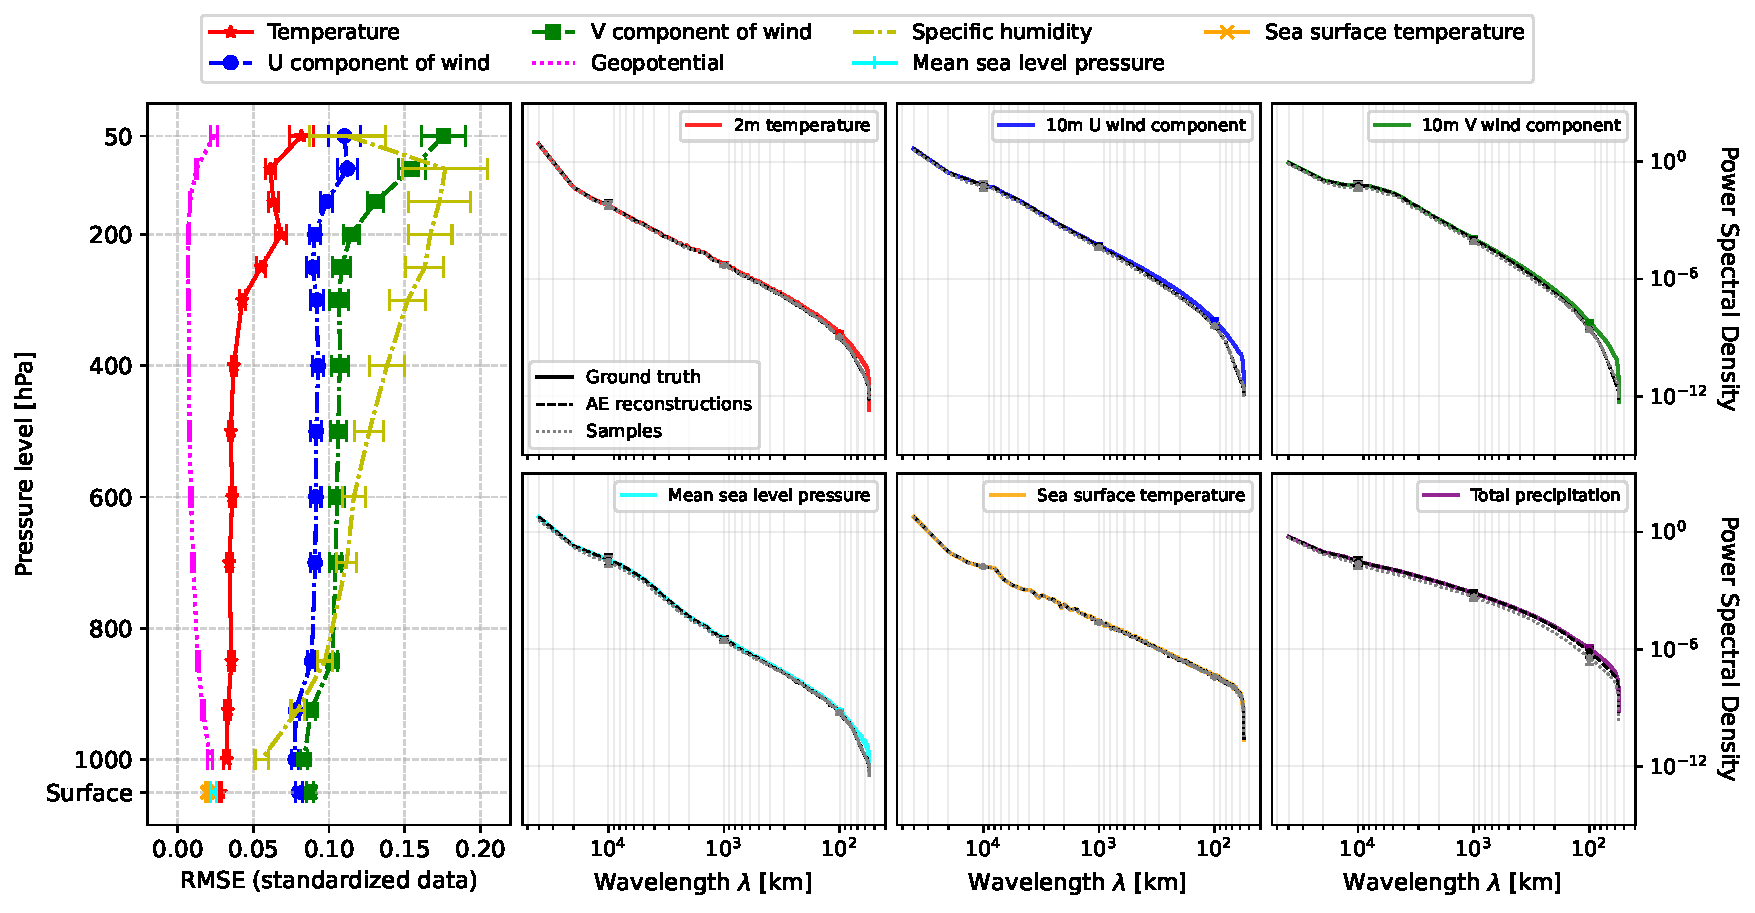
\includegraphics[width=\textwidth]{./chapters/appa/figures/ae_rmse_spectra.pdf}
    \caption{Standardized autoencoder reconstruction RMSE (left) and power spectra of Appa's prior samples (right) between January and December 2021. Lower-frequency fields (temperature, geopotential) are reconstructed more accurately than volatile fields (humidity, wind). Near-surface fields benefit from altitude-weighting. Power spectral density shows close alignment across wavelenghts, with deviations below \qty{100}{\kilo\meter}.}
    \label{fig:ae-rmse}
\end{figure}

\paragraph{Assimilation}
We evaluate Appa across four tasks: reanalysis, filtering, observational forecasting, and full-state forecasting. For the first three tasks, we assimilate synthetic ground station observations of all surface fields and simulated satellite scans of the 5 atmospheric fields. The station network consists of \num{11000} real-world measurement locations~\cite{noaanationalcentersofenvironmentalinformation1999global} covering roughly $\qty{1}{\percent}$ of \qty{0.25}{\degree} grid points. Ground stations are sparse and globally distributed, while satellite orbital paths provide dense coverage within a limited spatio-temporal domain. Observations are modeled as Gaussian distributions centered on the ERA5 ground-truth, with noise levels of $\qty{1}{\percent}$ for ground stations and $\qty{10}{\percent}$ for satellites, relative to the observed field's respective standard deviation. Each assimilation is carried with 10 ensemble members.

Figure~\ref{fig:reanalysis-quant} summarizes Appa's quantitative performance. Further results can be found in Appendix \ref{app:appa-additional-results}. For reanalysis and filtering, conditioning on longer assimilation windows improves both skill and CRPS but gains saturate beyond 24 hours. Forecasting's skill decays gradually with lead time but remains significantly stronger than the persistence baseline. Observational forecasts, conditioned on the last 12 hours of a day-long assimilation, start at skill and CRPS levels comparable to the reanalysis plateau. Full-state forecasts, initialized from two complete states, start with lower errors but eventually converge to similar performance. The error growth lies between two baselines: steeper than IFS~\cite{ecmwf2020ifs} but parallel to GraphDOP~\cite{alexe2024graphdop}. This suggests that the learned latent representation does not introduce artifacts that strongly impede the learning of the dynamics, supporting \textcite{rozet2025lost}'s findings.

\begin{figure}[!h]
    \centering
    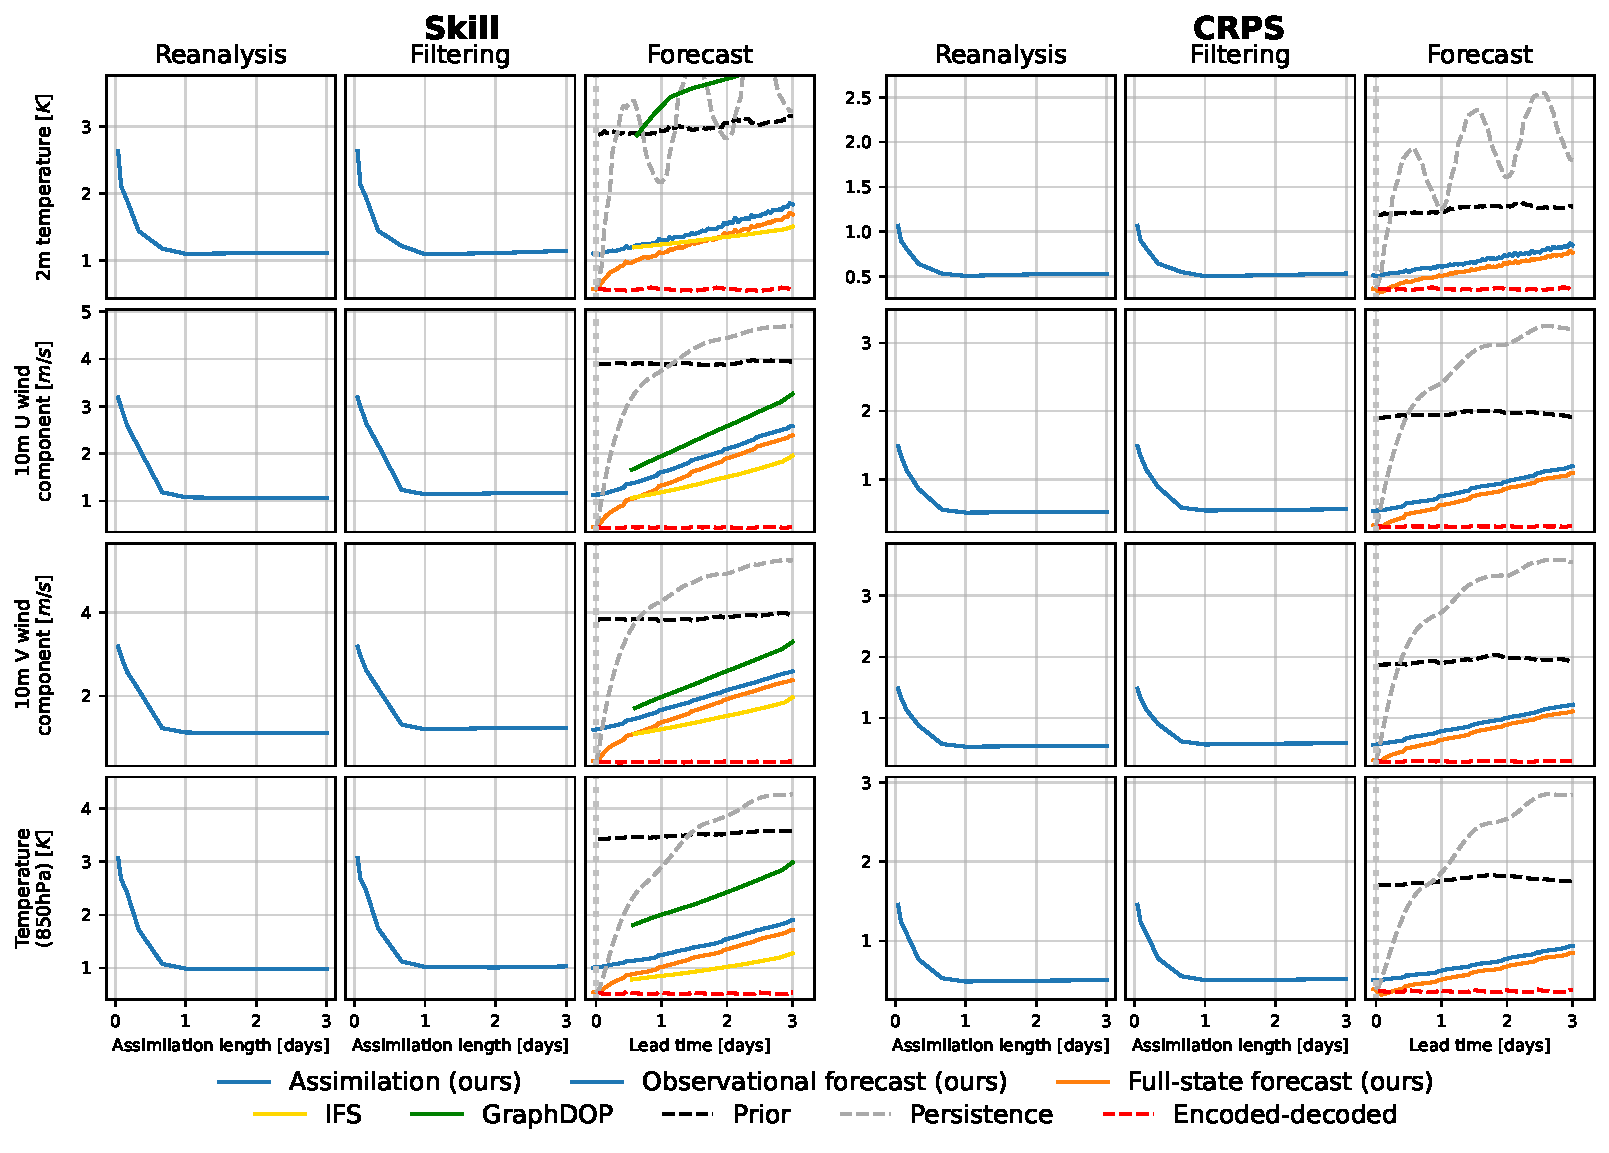
\includegraphics[width=\textwidth]{./chapters/appa/figures/skill_crps_main_2023.pdf}
    \caption{Skill and continuous ranked probability score (CRPS) of representative fields in assimilation tasks over January 2023. Reanalysis metrics are averaged over assimilation windows $x^{1:L}$, while filtering only considers the last assimilated state $x^L$. Both improve with longer assimilation windows, but eventually stagnate. Forecasts gradually lose skill over lead time. IFS~\cite{ecmwf2020ifs} and GraphDOP~\cite{alexe2024graphdop} are reported for reference.}
    \label{fig:reanalysis-quant}
\end{figure}

\section{Discussion} \label{sec:appa-discussion}

\paragraph{Summary}
We introduce Appa, a latent score-based data assimilation model that produces global atmospheric trajectories efficiently by operating in a compressed latent space. Appa can be conditioned on arbitrary observations without retraining, providing access to the full posterior distribution of consistent trajectories. Our results demonstrate that Appa flexibly handles reanalysis, filtering, and forecasting within a unified probabilistic framework, while remaining competitive with baselines.

\paragraph{Limitations and future work}
While Appa demonstrates strong assimilation and forecasting capabilities, it remains a proof of concept that isn't ready yet for operational applications. We foresee several possible improvements. First, we should move from simplified synthetic observations to realistic measurements, such as satellite radiances. Improving physical consistency is also critical, especially for forecasting tasks where Appa falls short of standard baselines such as IFS~\cite{ecmwf2020ifs}. Replacing guidance-based posterior sampling with explicit conditioning on past states, as in GenCast~\cite{price2025probabilistic} and LoLA~\cite{rozet2024learning}, could improve both accuracy and efficiency of forecasting. In terms of statistical assessment, the calibration of posterior distributions deserves further validation. The approximations present in our method, notably while estimating the prior and likelihood scores, introduce errors which are hard to quantify without proper statistical validation. Computational efficiency of reanalysis remains a challenge as well, as conditioning with respect to atmospheric observations requires decoding latent states repeatedly. Projecting observations into latent space could mitigate this bottleneck \cite{raphaeli2025silo}. Finally, our comparison to other models is still preliminary due to the discrepancies in experimental configurations. Fair evaluation against IFS~\cite{ecmwf2020ifs}, GraphDOP~\cite{alexe2024graphdop} and other models \cite{lam2023learning, price2025probabilistic} would help position Appa within the spectrum of global atmospheric models.

\section*{Acknowledgments}

Gérôme Andry, François Rozet, Sacha Lewin, and Elise Faulx are research fellows of the F.R.S.-FNRS (Belgium) and acknowledge its financial support. Omer Rochman acknowledges the financial support of the Walloon Region under grant no. 2.0102.35 (ARIAC by Digital Wallonia 4.AI). Victor Mangeleer is a research fellow part of the Multiple THreats on Ocean health (MiTHO) project and acknowledges funding from the European Space Agency (ESA).

The present research benefited from computational resources made available on Lucia, the Tier-1 supercomputer of the Walloon Region, infrastructure funded by the Walloon Region under the grant no. 1910247. The computational resources have been provided by the Consortium des Équipements de Calcul Intensif (CÉCI), funded by the Fonds de la Recherche Scientifique de Belgique (F.R.S.-FNRS) under the grant no. 2.5020.11 and by the Walloon Region.

\clearpage
\section*{References}

\printbibliography[heading=none]

\begin{subappendices}

\clearpage
\section{Data} \label{app:appa-data}

ERA5 is a global deterministic reanalysis dataset from ECMWF that provides high-resolution (\qty{0.25}{\degree}) hourly estimates of atmospheric, land, and oceanic fields from 1959 onward~\cite{hersbach2020era5}. It assimilates observations into a numerical weather prediction model using 4D-Var data assimilation.

In this work, we use a subset of ERA5 data, defined on a \qty{0.25}{\degree} equiangular grid with 13 pressure levels: 50, 100, 150, 200, 250, 300, 400, 500, 600, 700, 850, 925, and 1000 \unit{\hecto\pascal}. Following \textcite{lam2023learning}, we restrict the temporal coverage of the dataset to the 1993--2021 period, with data split into training (1993--2019), validation (2020), and testing (2021--2023). ERA5 data was downloaded from the WeatherBench2 \cite{rasp2024weatherbench} platform, where Google has made it available via Google Cloud Storage.

Table~\ref{tab:data-era5-fields} lists the selected fields. Some fields serve as both input and output (predicted) features, while others provide contextual information as inputs but are not predicted.

\begin{table}[h]
\centering
\caption{List of selected fields.}
\label{tab:data-era5-fields}
\begin{tabular}{ccc}
\toprule
\textbf{Type} & \textbf{Name} & \textbf{Role} \\
\midrule
Atmospheric & Temperature & Input / Output \\
Atmospheric & U-Wind Component & Input / Output \\
Atmospheric & V-Wind Component & Input / Output \\
Atmospheric & Geopotential & Input / Output \\
Atmospheric & Specific Humidity & Input / Output \\
Surface & 2m Temperature & Input / Output \\
Surface & 10m U-Wind Component & Input / Output \\
Surface & 10m V-Wind Component & Input / Output \\
Surface & Mean Sea Level Pressure & Input / Output \\
Surface & Sea Surface Temperature & Input / Output \\
Surface & Total Precipitation & Input / Output \\
\midrule
Time & Local time of day & Input (diffusion)\\
Time & Year progress & Input (diffusion)\\
\bottomrule
\end{tabular}
\end{table}

\subsection{Data processing}

\paragraph{Standardization} Although the dynamics across the atmospheric column are correlated, each pressure level exhibits distinct statistical behavior. Thus, we compute the mean and standard deviation separately for each field and at each pressure level, on the whole training dataset. We use these statistics to standardize our entire dataset and to rescale the output of Appa.

\paragraph{Missing values}
As sea surface temperature is undefined over land (NaN values), we replace these with zeros after standardization as a neutral placeholder.

\clearpage
\section{Technical details}

This section provides further technical details for training and inference. Our code will be made available with full reproducibility steps for both training and evaluation.

\subsection{Architectures}

We adapted architectures from \textcite{rozet2025lost} for both autoencoder and latent diffusion model. The encoder and decoder are fully convolutional neural networks and the diffusion model is adapted from a diffusion transformer (DiT) \cite{peebles2023scalable}.

\paragraph{Autoencoder}
The autoencoder compresses atmospheric states from the high-dimensional N320 grid ($721\times1440$ pixels with 71 channels) into a compact latent space ($23\times47$ pixels with 128 channels) via progressive spatial downsampling and channel expansion. To accommodate any spatial compression factor, the input is padded to the nearest compatible grid size. We apply circular padding along longitude to respect periodicity, and constant zero padding along latitude to handle polar boundaries. The encoder-decoder pair is trained with a latitude-altitude-weighted mean squared error loss, following \textcite{lam2023learning}.

\begin{table}[!h]
    \centering
    \caption{Autoencoder training configuration}
    \begin{tabular}{ll}
        \toprule
        \textbf{Parameter} & \textbf{Value} \\
        \midrule
        Loss function & latitude-altitude-weighted mean squared error \\
        Latent noise & $\sigma_z = 0.01$ for regularization \\
        Optimizer & SOAP \cite{vyas2025soap} with initial learning rate \num{3e-5} and linear decay\\
        Batch size & 64 samples per optimizer step \\
        Training duration & 95000 optimizer steps (2 days) \\
        Hardware & 64 A100 (40GB) GPUs \\
        \bottomrule
    \end{tabular}
    \label{tab:training-details}
\end{table}

\paragraph{Latent denoiser}
The denoiser is a DiT that operates on $W = 24$ consecutive latent states. We patchify the latent sequence by a factor of 2 along the temporal axis and flatten the spatial dimensions, yielding a total of $23 \times 47 \times \nicefrac{24}{2} = \num{12972}$ tokens, each with 256 channels. During training and inference, we adopt a variance exploding noise process \cite{song2019generative} for which $\alpha_t = 1$ and $\sigma_t \in [\sigma_{\min}, \sigma_{\max}]$.

\begin{table}[!h]
    \centering
    \caption{Denoiser training configuration}
    \begin{tabular}{ll}
        \toprule
        \textbf{Parameter} & \textbf{Value} \\
        \midrule
        Loss & Denoising score matching \\
        Noise range & $\sigma_{\min} = \num{e-3}$, $\sigma_{\max} = \num{e3}$ \\
        Optimizer & Adam \cite{kingma2015adam} with initial learning rate \num{e-4} \\
        Batch size & 256 samples per optimizer step\\
        Training duration & 125000 optimizer steps (5 days) \\
        Hardware & 64 A100 (40GB) GPUs \\
        \bottomrule
    \end{tabular}
    \label{tab:denoiser-training}
\end{table}

\subsection{Assimilation}

\paragraph{Forecasting}
Appa is trained to generate state windows of $W = 24$ hours. To perform forecasting, we split the window in two parts: the conditioned states and the predicted states. We either use the result of a reanalysis (observational forecasting) or encoded ground-truth atmospheric states (full-state forecasting) as condition, to infer the first window. For forecast of more than 24 hours, we perform autoregressive rollout. We use the last latent states of the previous window to condition the next one. The number of conditioning states can be tuned to carry more or less information from the past states.

\paragraph{Evaluation}
In Figure \ref{fig:reanalysis-quant}, we borrow IFS~\cite{ecmwf2020ifs} and GraphDOP \cite{alexe2024graphdop} metrics from \textcite{alexe2024graphdop}. However, a direct and fair comparison is difficult due to the lack of experimental details. \textcite{alexe2024graphdop} report metrics for 6 different fields over January 2023, but do not mention the exact dates or ensemble size. We selected the first 8 days of January 2023 at midnight as starting time. We compute metrics for 10 ensemble members.

\section{Evaluation metrics}

We follow conventional metrics for assimilation and forecasting performance. For a fair comparison with the literature, evaluation is performed using WeatherBench2 \cite{rasp2024weatherbench}. For assimilation, we average performance over the time steps.

\paragraph{Skill}
The skill \cite{fortin2014why, price2025probabilistic} of an ensemble of $K$ particles $v_k$ is defined as the RMSE of the ensemble mean compared to the ground-truth $u$
\begin{equation}
    \text{Skill} = \sqrt{\left\langle \left( u - \frac{1}{K} \sum_{k=1}^K v_k \right)^2 \right\rangle}
\end{equation}
where $\langle \cdot \rangle$ denotes the spatial mean operator.

\paragraph{Spread} The spread \cite{fortin2014why, price2025probabilistic} is defined as the ensemble standard deviation
\begin{equation}
    \text{Spread} = \sqrt{\left\langle \frac{1}{K - 1} \sum_{j=1}^K \left( v_j - \frac{1}{K} \sum_{k=1}^K v_k \right)^2 \right\rangle}
\end{equation}

\paragraph{Spread-Skill ratio} Under these definitions and the assumption of a perfect forecast where ensemble particles are exchangeable, \textcite{fortin2014why} show that
\begin{equation}
    \text{Skill} = \sqrt{\frac{K + 1}{K}} \text{Spread}
\end{equation}
This motivates the use of the (corrected for ensemble size) spread-skill ratio as a metric. Intuitively, if the ratio is smaller than one, the ensemble is biased or under-dispersed. If the ratio is larger than one, the ensemble is over-dispersed. It should be noted, however, that a spread-skill ratio of 1 is a necessary but not sufficient condition for a perfect forecast.

\paragraph{CRPS} The continuous ranked probability score (CRPS) \cite{hersbach2000decomposition, gneiting2007strictly} is defined as
\begin{equation}
    \text{CRPS} = \left\langle \frac{1}{K} \sum_{k=1}^K | u - v_k | - \frac{1}{2K(K - 1)} \sum_{j=1}^K \sum_{k=1}^{K} | v_j - v_k | \right\rangle
\end{equation}
The first term penalizes the distance of the particles to the ground-truth while the second term encourages variations within the ensemble. Minimizing the CRPS ($\text{CRPS} = 0$) means that the 1-d marginals of the ensemble are calibrated.

\clearpage
\section{Additional results} \label{app:appa-additional-results}

\begin{figure}[!h]
    \centering
    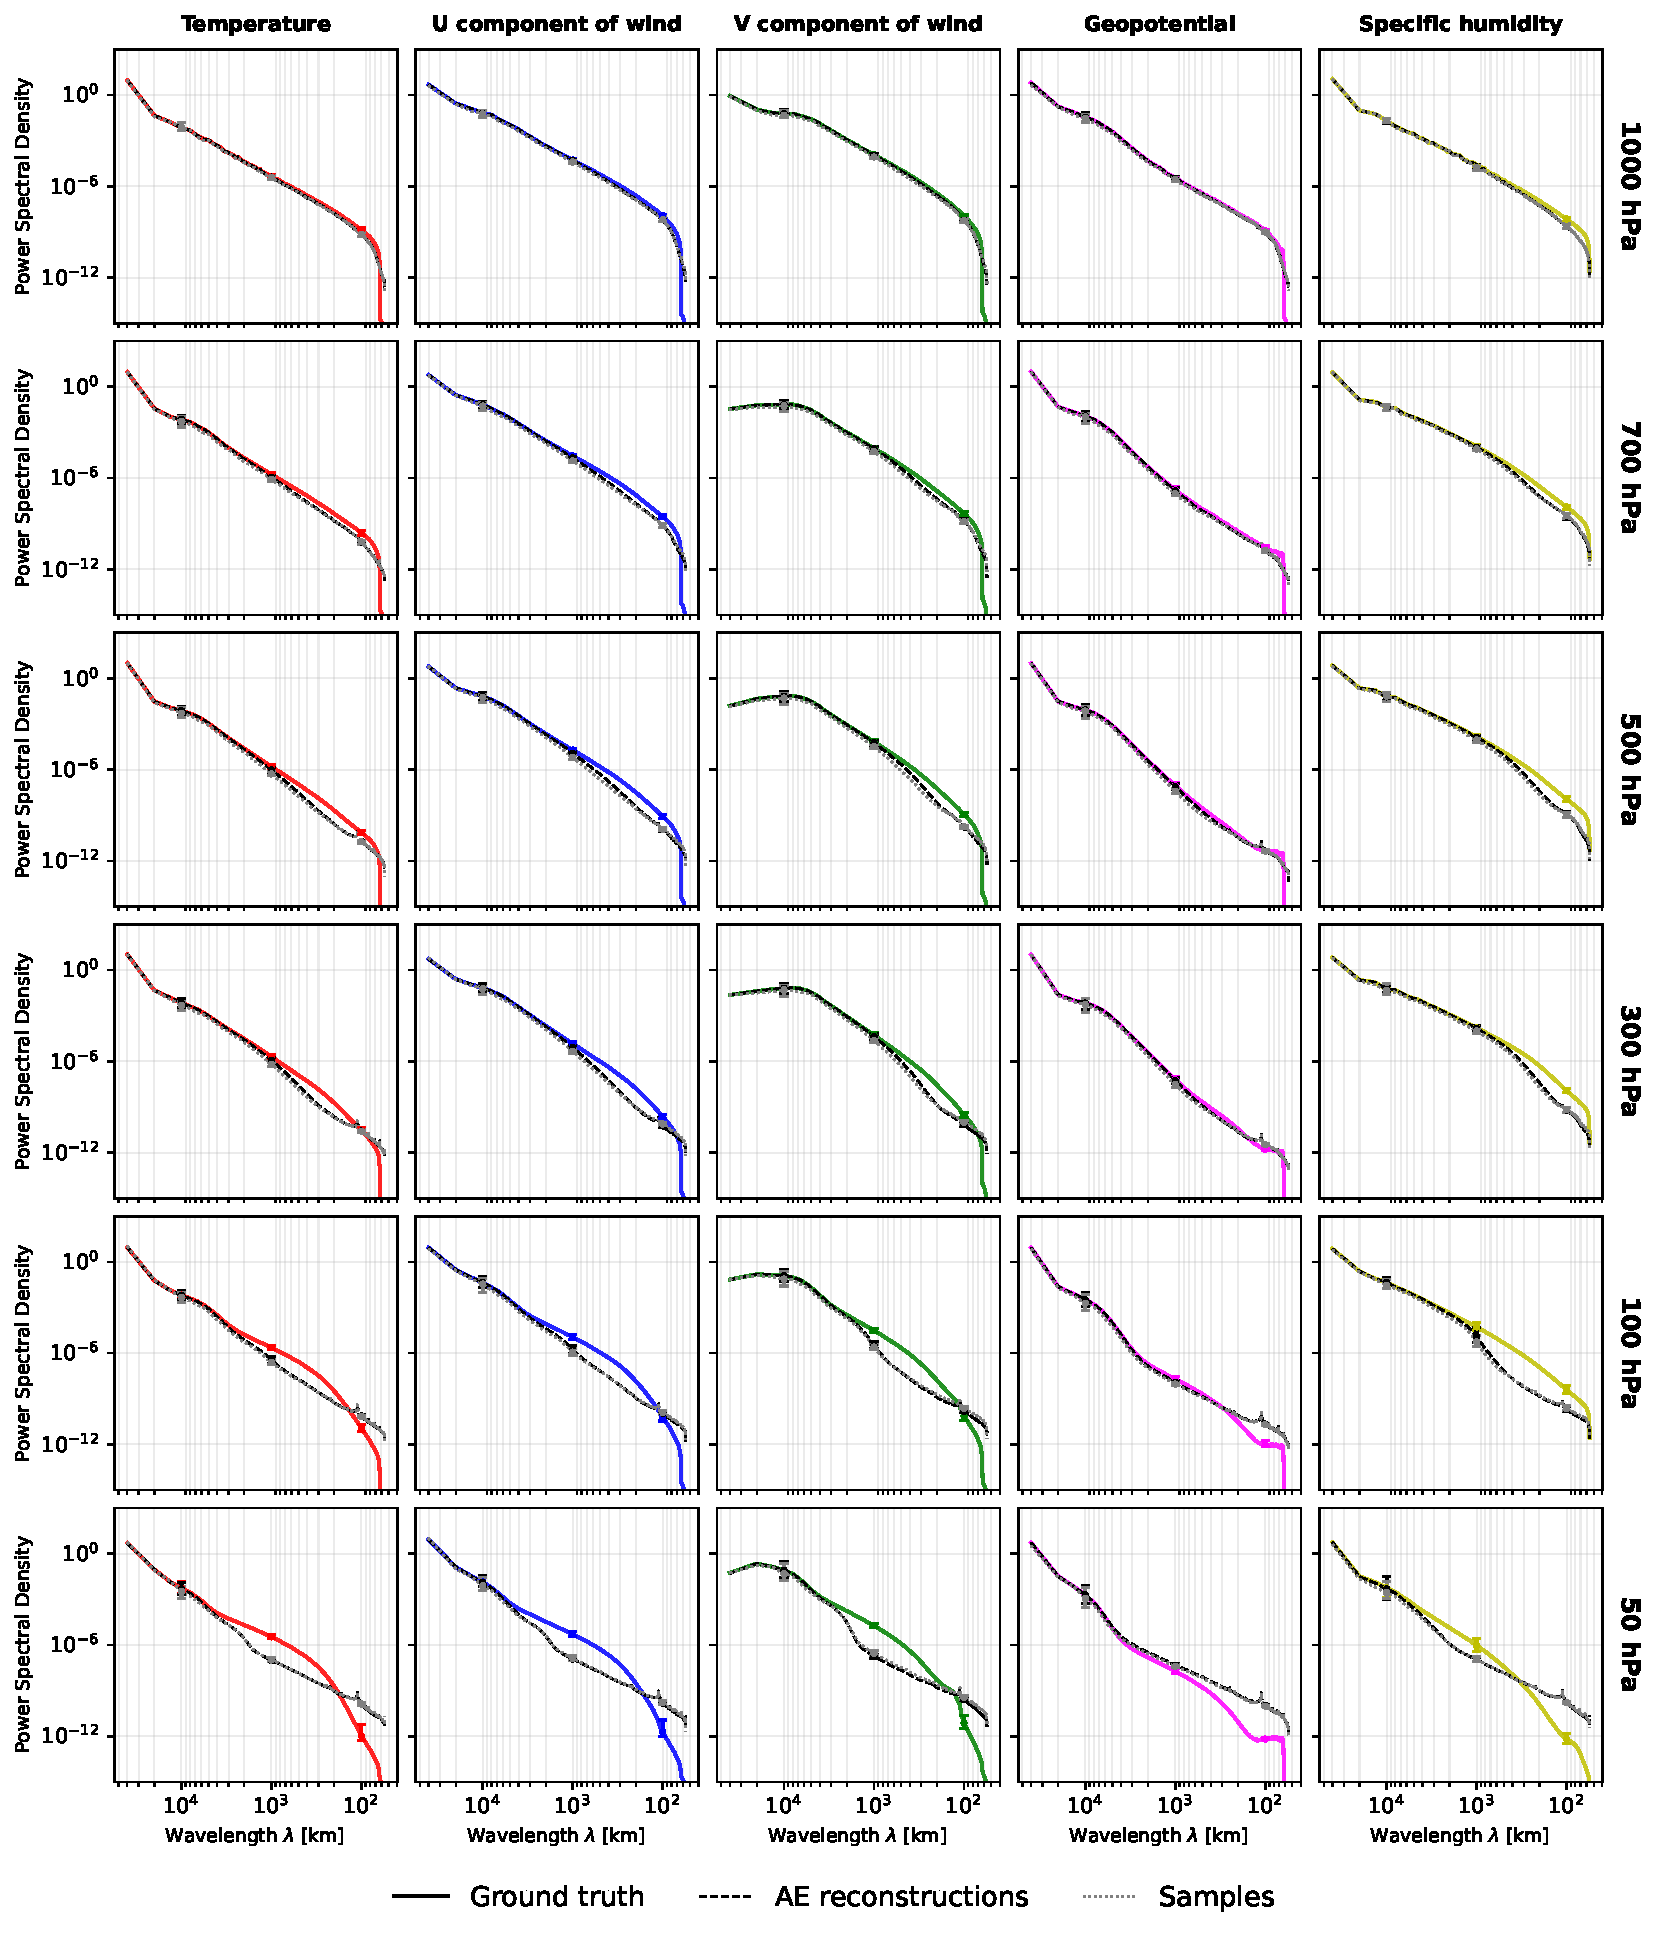
\includegraphics[width=\textwidth]{./chapters/appa/figures/power_spectra.pdf}
    \caption{Power spectral density across wavelengths for atmospheric fields at different pressure levels between January 2021 and December 2021. Lines show median values and error bars indicate the 5th to 95th percentiles. The close alignment between the curves demonstrates that both the autoencoder and the diffusion model preserve the energy distribution across most spatial scales. Deviations begin to appear at wavelengths around \qty{1000}{\kilo\meter}, which corresponds to roughly 40 pixels at the equator at our \qty{0.25}{\degree} resolution. These differences become more pronounced at smaller scales, suggesting that while large-scale atmospheric patterns are well-preserved, features spanning fewer than \qty{1000}{\kilo\meter} lose energy in the compression processes. Deviations become more pronounced at lower pressure levels, as the model prioritizes surface and low-altitude fields.}
\end{figure}

\begin{figure}[!h]
    \centering
    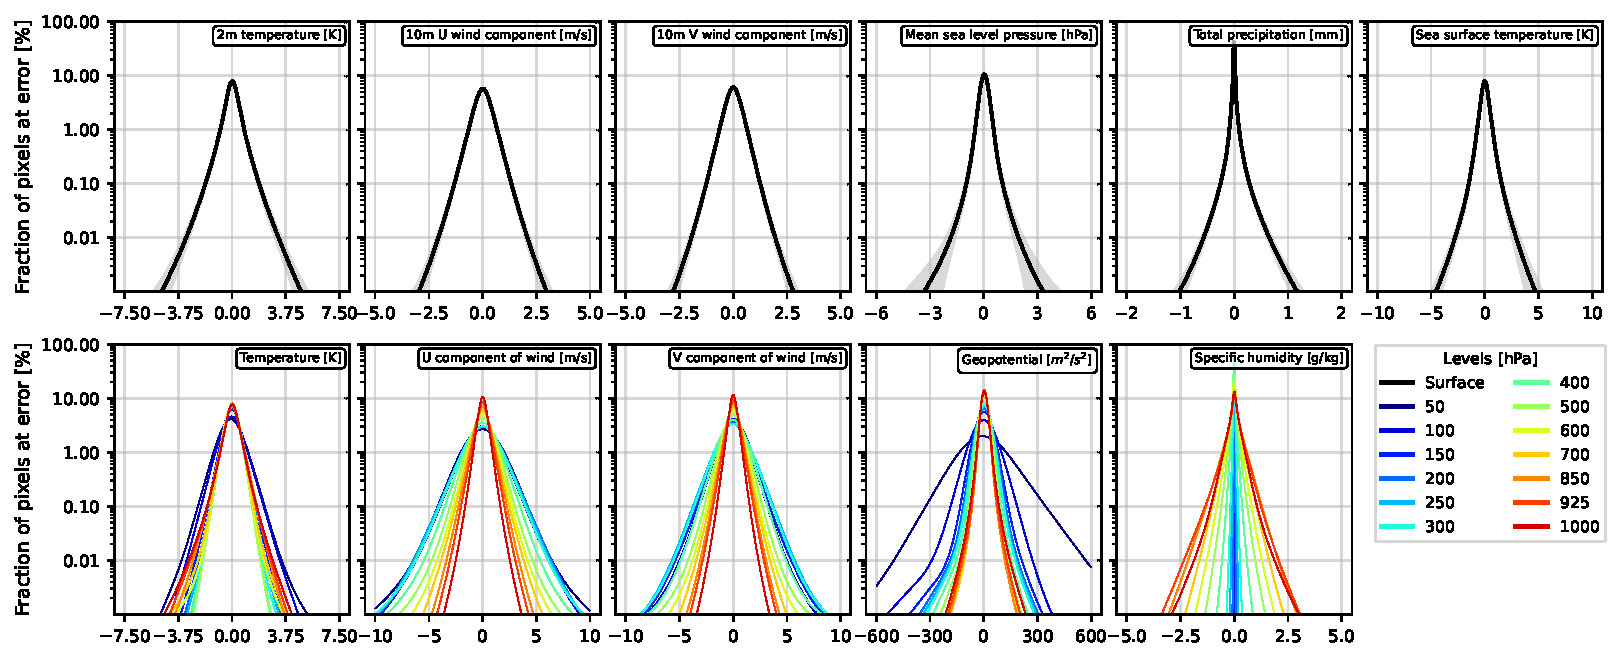
\includegraphics[width=\textwidth]{./chapters/appa/figures/ae_bells.pdf}
    \caption{Reconstruction bias distributions for surface fields across all grid points (top) and atmospheric fields across all pressure levels (bottom). The distributions centered around zero demonstrate unbiased and accurate reconstructions. For $\num{721} \times \num{1440} = \num{1038240}$ grid points, a \qty{0.01}{\percent} fraction on the y-axis corresponds to approximately 100 points, indicating that large biases are rare.}
    \label{fig:ae-bias}
\end{figure}

\begin{figure}[!h]
    \centering
    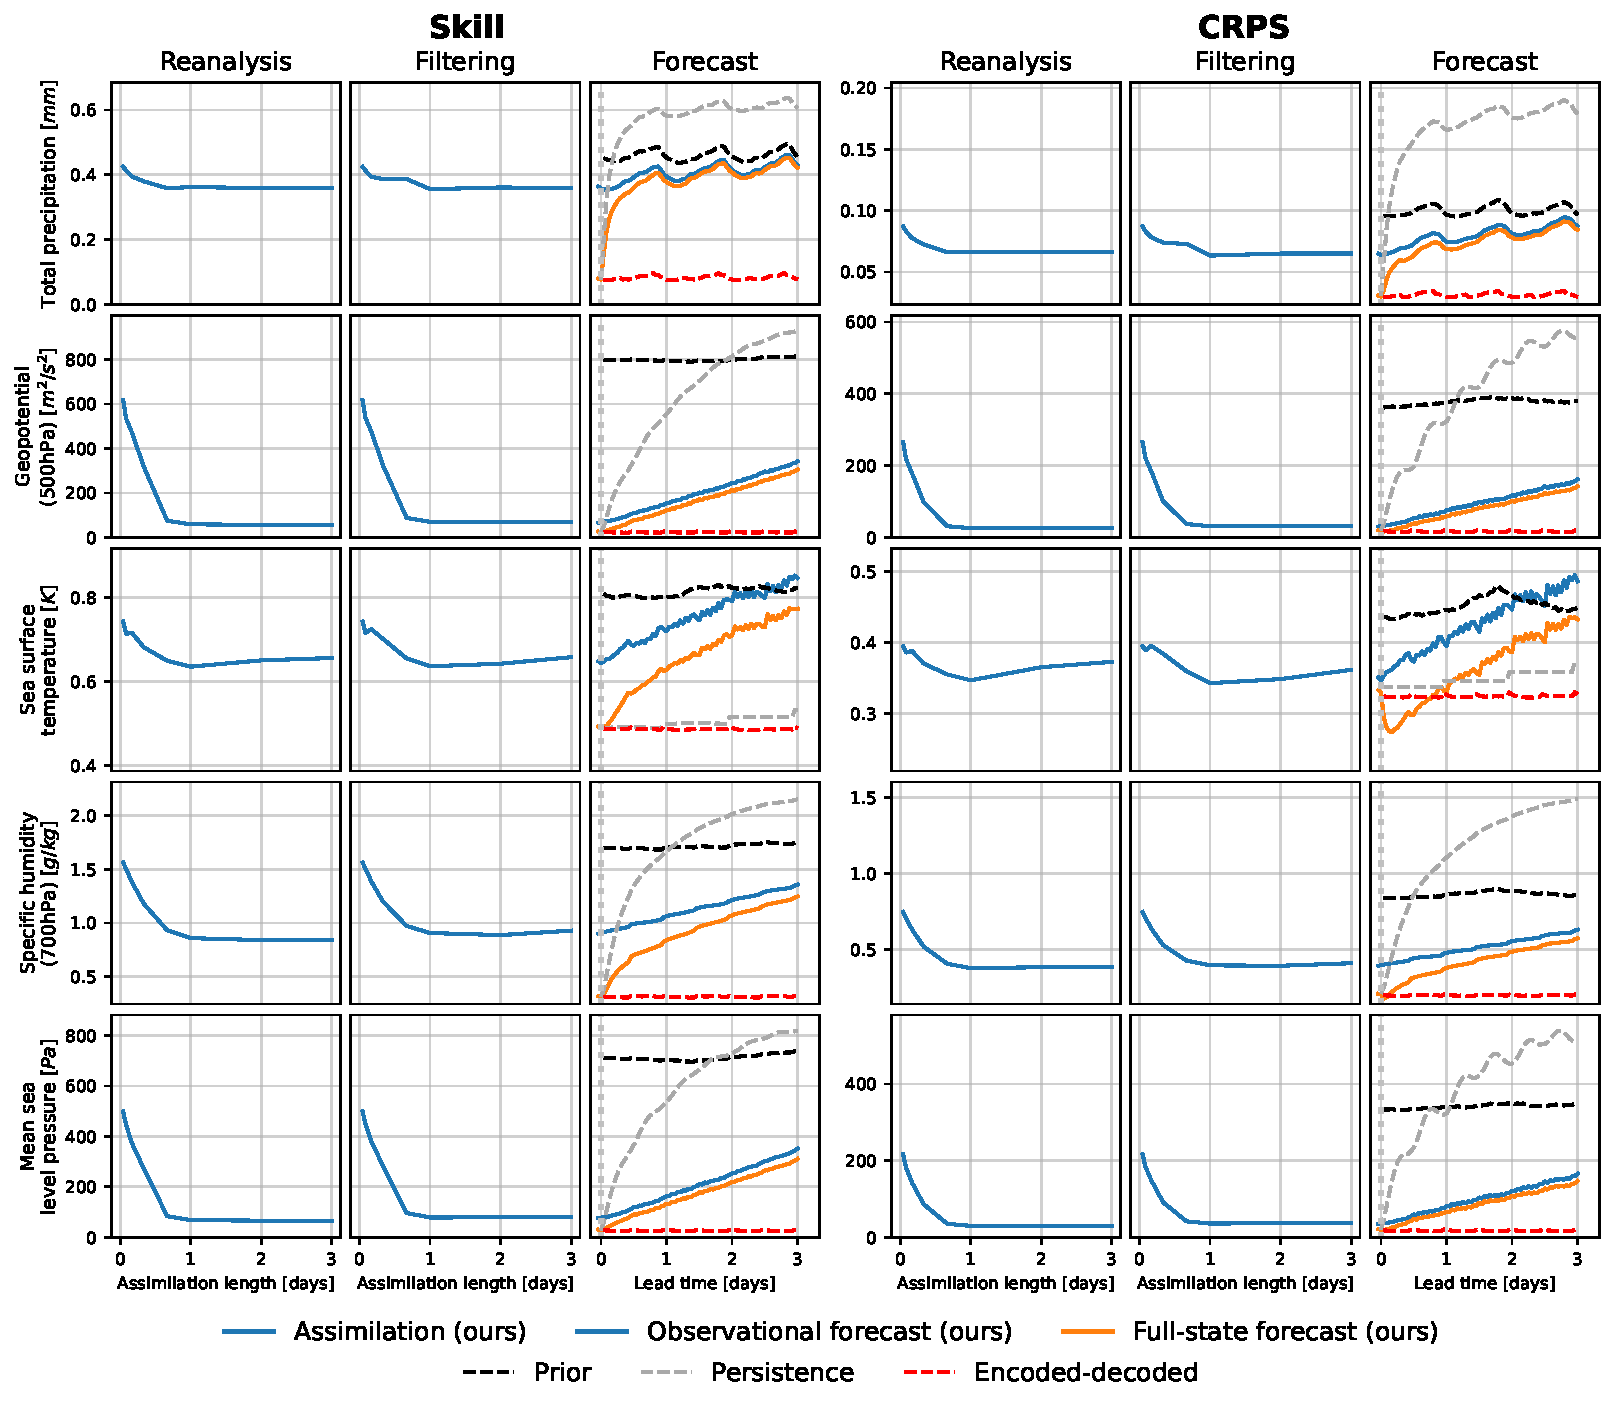
\includegraphics[width=\textwidth]{./chapters/appa/figures/skill_crps_appendix_2023.pdf}
    \caption{Skill and CRPS of other representative fields in assimilation tasks over January 2023. Reanalysis metrics are averaged over assimilation windows $x^{1:L}$, while filtering only considers the last assimilated state $x^L$. Both improve with longer assimilation windows, but eventually stagnate. Forecasts gradually lose skill over lead time. IFS~\cite{ecmwf2020ifs} and GraphDOP~\cite{alexe2024graphdop} are shown for reference.}
\end{figure}

\begin{figure}[!h]
    \centering
    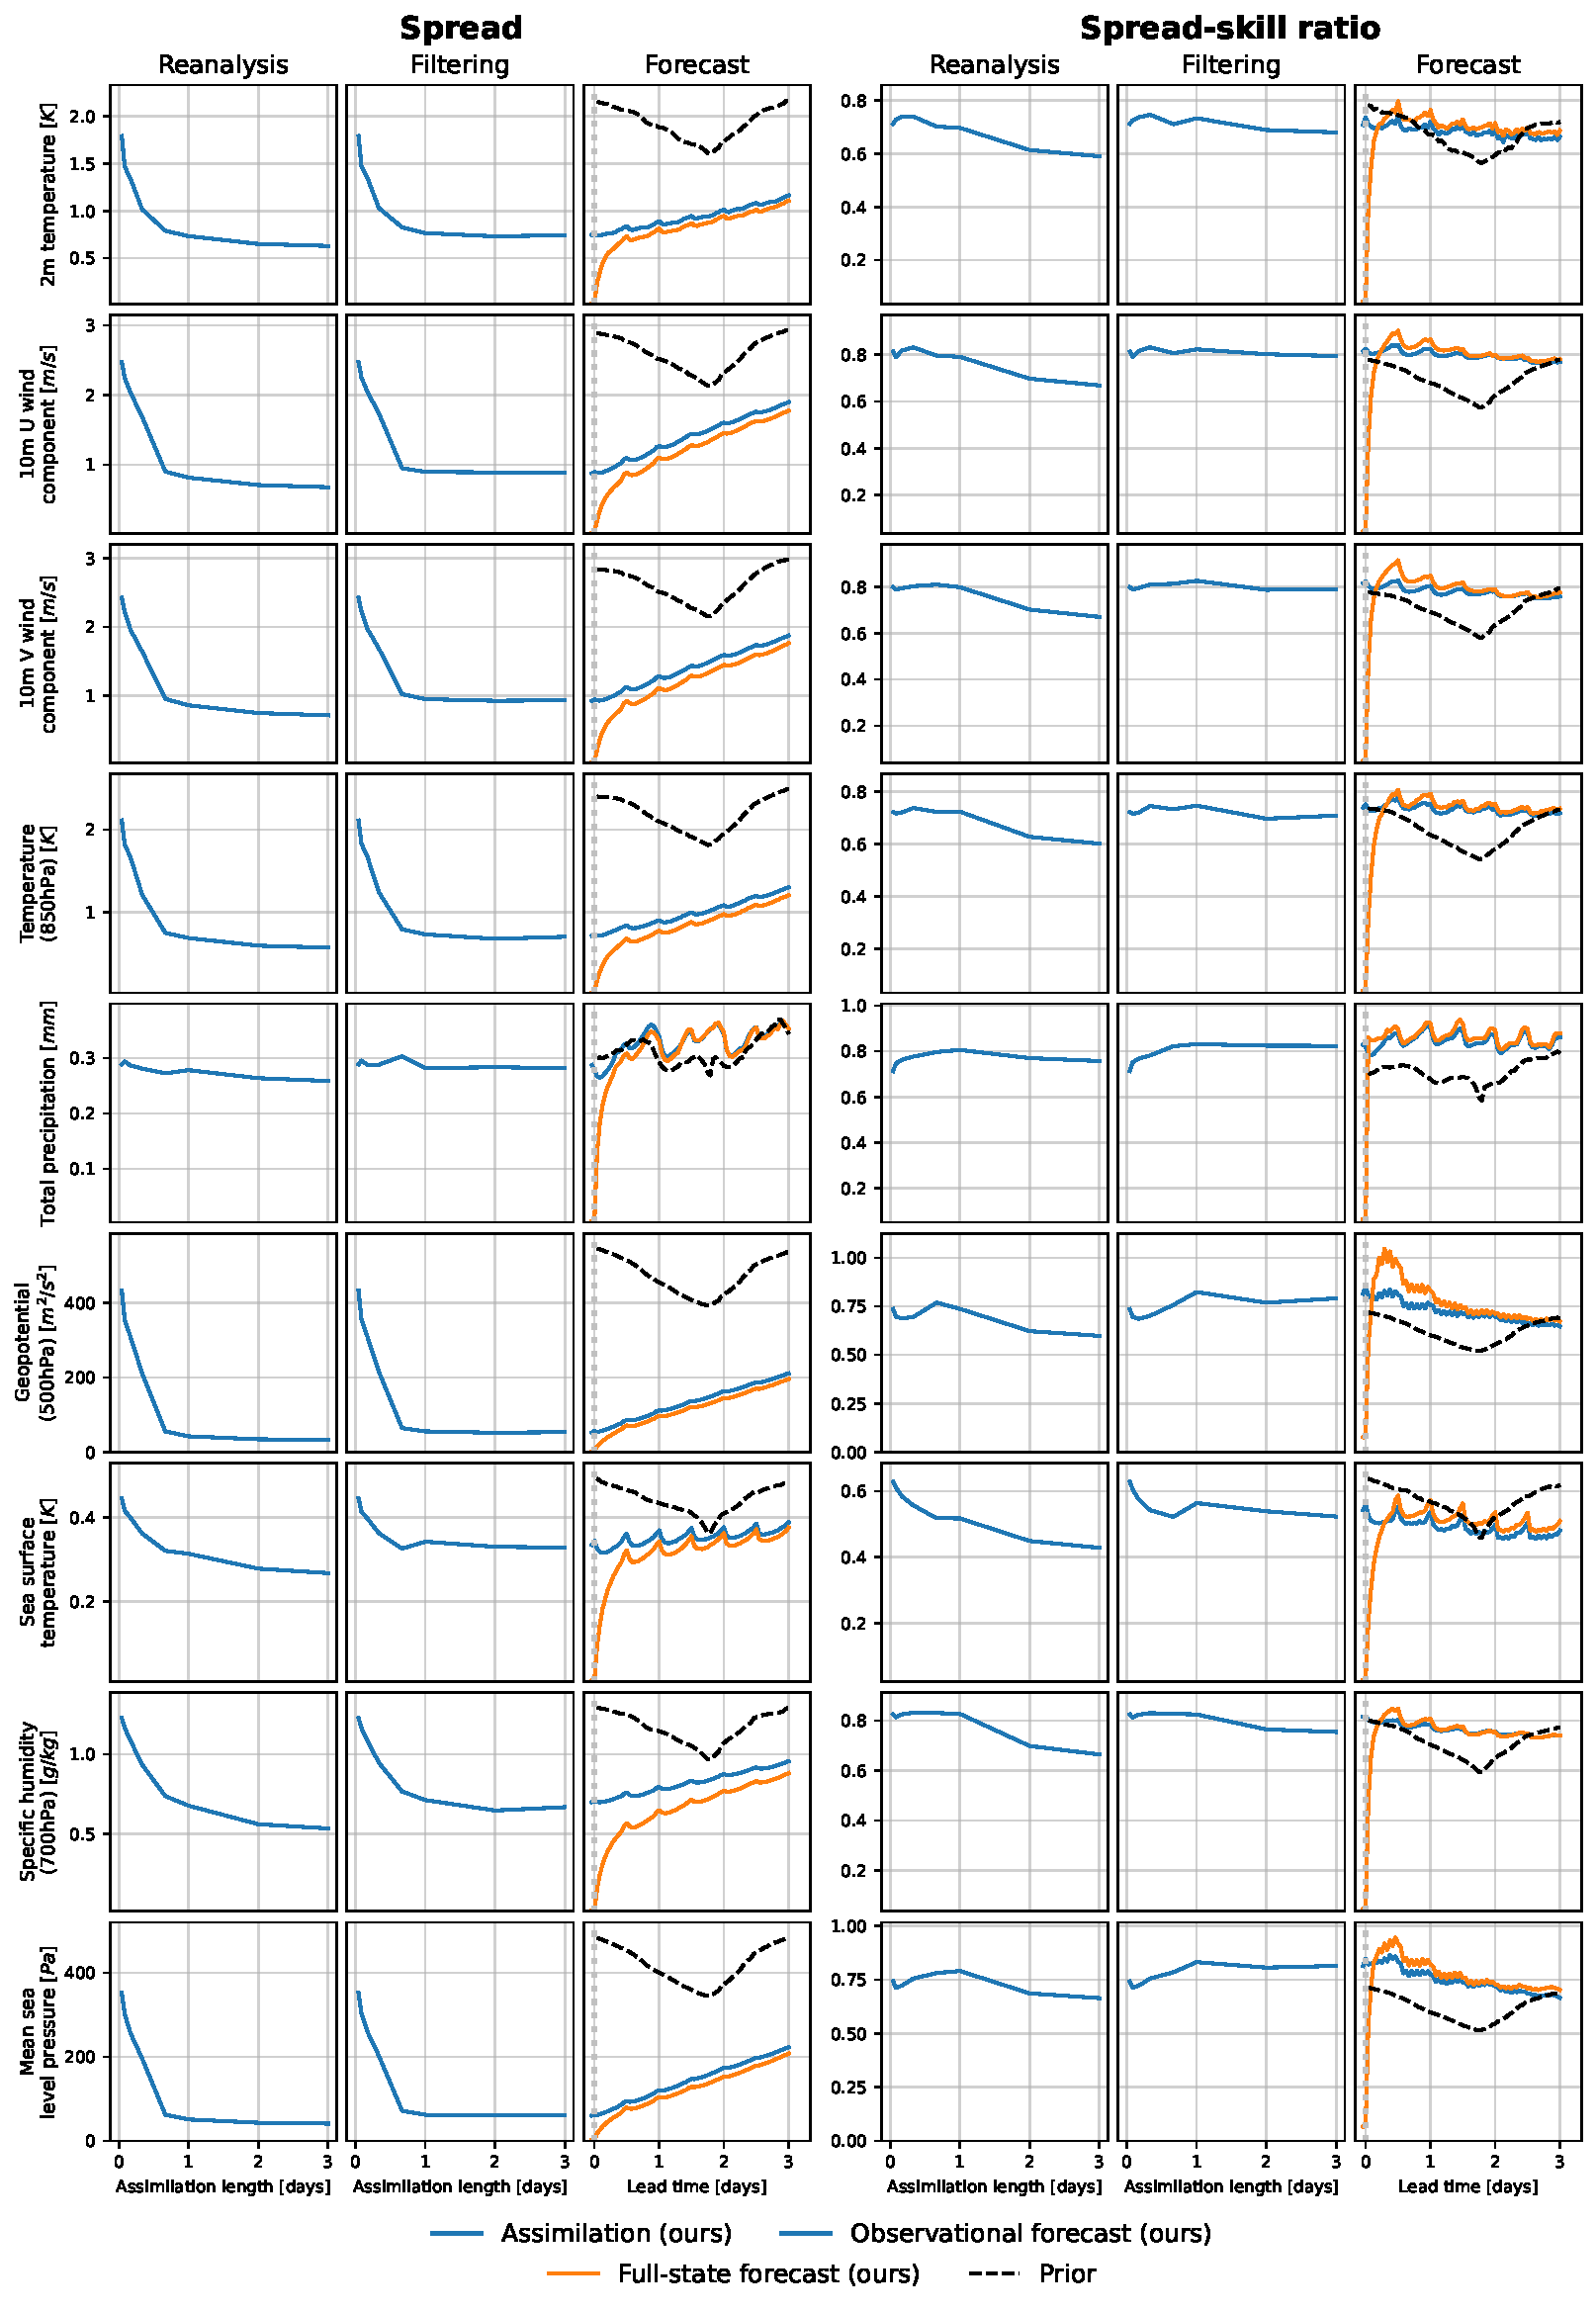
\includegraphics[width=\textwidth]{./chapters/appa/figures/spread_skill_ratio_2023.pdf}
    \caption{Spread and Spread-Skill ratio of representative fields in assimilation tasks over January 2023. Metrics are averaged over assimilation windows $x^{1:L}$, while filtering only considers the last assimilated state $x^L$. Ensemble spread (i.e. uncertainty) decreases with longer assimilation windows, while spread-skill ratios remain constant. A ratio below one indicates overconfidence.}
\end{figure}

\clearpage
\subsection{Physical consistency}

To further evaluate physical consistency, we examine whether our model preserves important physical relationships between variables. First, we analyze the consistency between two different estimators of altitude at given pressure levels. Using the geopotential $\Phi$, altitude can be derived as
\begin{equation}
    H = \frac{\Phi R_e}{g_{0}R_e-\Phi} \, ,
\end{equation}
where $R_e$ is Earth's radius and $g_{0}$ is the Earth gravitational acceleration at the surface. Alternatively, the equation below (which relies on the ideal gas law and hydrostatic equation) relates altitude to pressure and temperature as
\begin{equation}
    \log{\frac{p_0}{p_H}} = \frac{M g_0}{R}\int_0^H \frac{1}{T_h} \partial{h} \, ,
\end{equation}
where $R$ is the universal gas constant, $M$ is an approximation of the atmosphere's molar mass, $p_h, T_h$ are pressure and temperature at height $h$, and $p_0$, $T_0$ are the theoretical pressure and temperature at sea level. This integral can be approximated to extract $H$ using several assumptions about the temperature profile. When comparing these two estimators, Figure~\ref{fig:physical-consistency} shows that our generated samples maintain the same systematic differences $\Delta H$ as seen in ground-truth data. This remarkable consistency indicates that our model successfully preserves this physical relationships between temperature, pressure, and geopotential, allowing altitude to be estimated through two independent methods with nearly identical accuracy to the original ERA5 data.

Second, we examine the geostrophic balance
\begin{align}
    \frac{\partial \Phi}{\partial x} & = \frac{4 \pi \Omega R_e}{N_x} \sin{\phi} \cos{\phi} u_g\\
    \frac{\partial \Phi}{\partial y} & = -\frac{2 \pi \Omega R_e}{N_y} \sin{\phi} v_g
\end{align}
which is the theoretical equilibrium between pressure gradient forces and Coriolis forces that governs large-scale atmospheric motion. In the above system, $\phi$ is the latitude, $N_x$ and $N_y$ are the number of pixels along longitude and latitude, $\Omega$ is the magnitude of the Earth's angular velocity, and $u_g$ and $v_g$ denote the eostrophic components of the wind. In this balance, in the absence of vertical motion, friction, and isobaric curvature, wind direction should be perpendicular to geopotential gradients, with wind speed proportional to gradient magnitude. This relationship can be expressed by comparing two quantities: (1) the angle $\theta$ between wind and geopotential gradients, which should approach \qty{90}{\degree} in geostrophic conditions, and (2) the correlation between wind speed magnitude and geopotential gradient magnitude, which should approach 1 in perfect geostrophic balance. Figure~\ref{fig:physical-consistency} shows that our generated samples accurately reproduce both aspects of this relationship. At \qty{500}{\hecto\pascal}, the approximate level of non-divergence with minimal surface friction effects, both ERA5 data and our generated samples show angles concentrated around \qty{90}{\degree}. Near the surface at \qty{1000}{\hecto\pascal}, where additional forces become significant, both datasets show a systematic deviation in angle. Similarly, the correlation between wind speed and geopotential gradient magnitudes in our samples closely matches the patterns observed in ERA5 data, exhibiting imperfect correlation only at lower pressure levels (explained by the level-weighted training) and following the same decreasing trend as pressure increases toward the surface, where ageostrophic components become more prominent.

These results demonstrate that our latent diffusion model not only preserves the statistical properties of atmospheric fields but also maintains important physical relationships between variables producing trajectories that are physically consistent and realistic. While these analyses confirm strong spatial consistency and physical fidelity, future work should extend our evaluation to more thoroughly quantify the temporal consistency of generated trajectories.

\begin{figure}[!h]
    \centering
    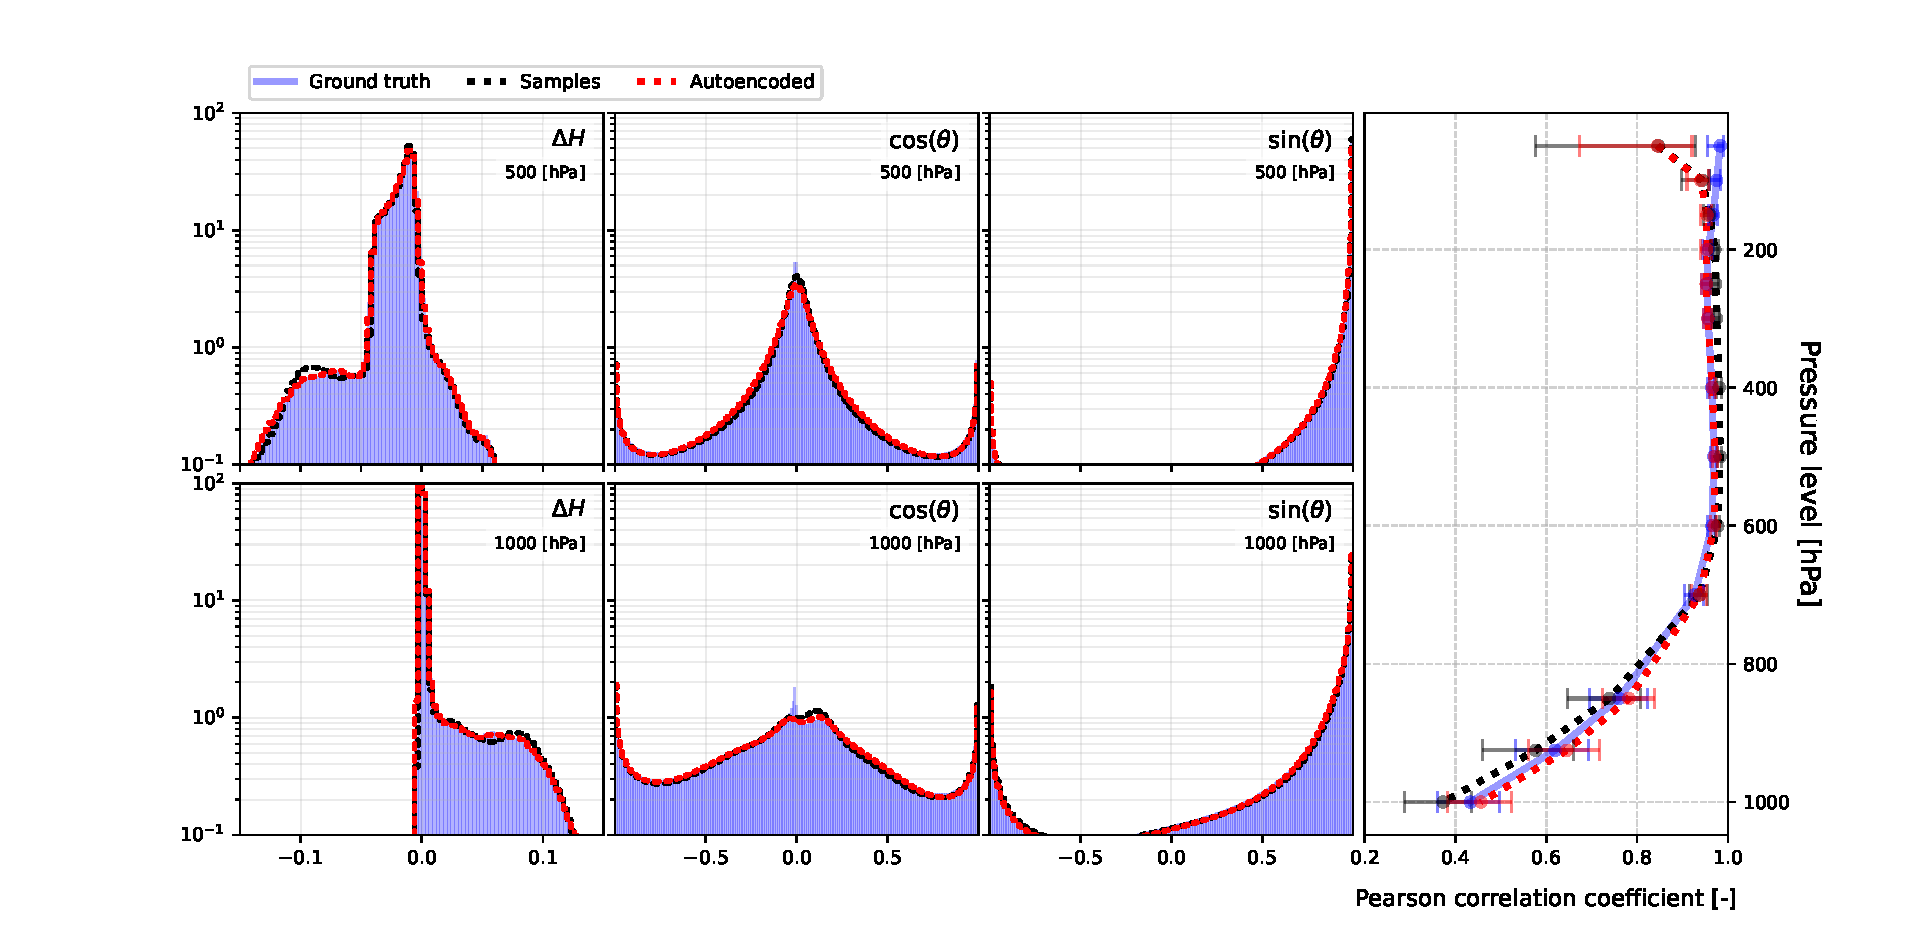
\includegraphics[width=\textwidth]{./chapters/appa/figures/physical_consistency.pdf}
    \caption{Physical consistency analysis of generated atmospheric states.
    \textbf{(top)} Analysis of altitude consistency at \qty{500}{\hecto\pascal} showing the difference $\Delta H$ between two independent altitude estimators, and geostrophic balance assessment through the cosine and sine of the angle $\theta$ between wind direction and geopotential gradients, demonstrating angles concentrated around \qty{90}{\degree}.
    \textbf{(bottom)} Same metrics at \qty{1000}{\hecto\pascal} demonstrating the presence of a significant ageostrophic component near the surface.
    \textbf{(right)} Correlation coefficient between wind magnitude and geopotential gradient magnitude across pressure levels, showing strong correlation at upper levels (near 1) with a consistent decrease toward the surface in both ERA5 data (blue) and generated samples (black dots), confirming Appa's ability to capture complex physical relationships.}
    \label{fig:physical-consistency}
\end{figure}

\clearpage
\subsection{Qualitative snapshots}

In Figures \ref{fig:gallery_t2m} to \ref{fig:gallery_z850}, we illustrate trajectories generated through reanalysis over a window of $L=72$ hours or through forecasting, for six representative fields. The second row of each gallery shows the observed pixels, if any. Surface fields and atmospheric fields have different observation masks (ground station network vs. satellite orbital).

\begin{figure}[!h]
    \centering
    \includegraphics[width=\textwidth]{./chapters/appa/compressed/gallery/reanalysis/2m_temperature.pdf}
    \includegraphics[width=\textwidth]{./chapters/appa/compressed/gallery/forecasting/2m_temperature.pdf}
    \caption{Sampled trajectories for surface temperature assimilation. Reanalysis (top) and observational forecasting (bottom) over a window of 72 hours.}
    \label{fig:gallery_t2m}
\end{figure}

\begin{figure}
    \centering
    \includegraphics[width=\textwidth]{./chapters/appa/compressed/gallery/reanalysis/10m_u_component_of_wind.pdf}
    \includegraphics[width=\textwidth]{./chapters/appa/compressed/gallery/forecasting/10m_u_component_of_wind.pdf}
    \caption{Sampled trajectories for surface zonal wind speed assimilation. Reanalysis (top) and observational forecasting (bottom) over a window of 72 hours.}
    \label{fig:gallery_10u}
\end{figure}

\begin{figure}
    \centering
    \includegraphics[width=\textwidth]{./chapters/appa/compressed/gallery/reanalysis/10m_v_component_of_wind.pdf}
    \includegraphics[width=\textwidth]{./chapters/appa/compressed/gallery/forecasting/10m_v_component_of_wind.pdf}
    \caption{Sampled trajectories for surface meridional wind speed assimilation. Reanalysis (top) and observational forecasting (bottom) over a window of 72 hours.}
    \label{fig:gallery_10v}
\end{figure}

\begin{figure}
    \centering
    \includegraphics[width=\textwidth]{./chapters/appa/compressed/gallery/reanalysis/total_precipitation.pdf}
    \includegraphics[width=\textwidth]{./chapters/appa/compressed/gallery/forecasting/total_precipitation.pdf}
    \caption{Sampled trajectories for total precipitation assimilation. Reanalysis (top) and observational forecasting (bottom) over a window of 72 hours.}
    \label{fig:gallery_tp}
\end{figure}

\begin{figure}
    \centering
    \includegraphics[width=\textwidth]{./chapters/appa/compressed/gallery/reanalysis/specific_humidity_700hPa.pdf}
    \includegraphics[width=\textwidth]{./chapters/appa/compressed/gallery/forecasting/specific_humidity_700hPa.pdf}
    \caption{Sampled trajectories for specific humidity assimilation at \qty{700}{\hecto\pascal}. Reanalysis (top) and observational forecasting (bottom) over a window of 72 hours.}
    \label{fig:gallery_q700}
\end{figure}

\begin{figure}
    \centering
    \includegraphics[width=\textwidth]{./chapters/appa/compressed/gallery/reanalysis/geopotential_850hPa.pdf}
    \includegraphics[width=\textwidth]{./chapters/appa/compressed/gallery/forecasting/geopotential_850hPa.pdf}
    \caption{Sampled trajectories for geopotential assimilation at \qty{850}{\hecto\pascal}. Reanalysis (top) and observational forecasting (bottom) over a window of 72 hours.}
    \label{fig:gallery_z850}
\end{figure}

\end{subappendices}


\newgeometry{margin=2.5cm, footskip=1cm, includefoot}
\cleardoublepage
\part{Epilogue} \label{part:epilogue}
\restoregeometry

\chapter{Discussion} \label{chap:discussion}

\begin{quote}
    \textit{The view that machines cannot give rise to surprises is due, I believe, to a fallacy to which philosophers and mathematicians are particularly subject. This is the assumption that as soon as a fact is presented to a mind, all consequences of that fact spring into the mind simultaneously with it. It is a very useful assumption under many circumstances, but one too easily forgets that it is false. A natural consequence of doing so is that one then assumes that there is no virtue in the mere working out of consequences from data and general principles.}

    \begin{flushright}
        --- Alan Turing (1950) \nocite{turing1950computing}
    \end{flushright}
\end{quote}

\vspace{1em}

As this dissertation reaches its final chapter, we take a moment to look both backward and forward. Throughout this work, we investigate the application of generative models to large-scale inference problems in physics, focusing in particular on systems whose states evolve over time. Such dynamical systems are ubiquitous in nature, science, and engineering and thus constitute a key research area for technological and societal progress. Across the five preceding chapters, we explore multiple facets of probabilistic modeling and dynamical systems, including state estimation, forecasting, reduced-order modeling, and learning from corrupted observations. We now pause to reflect on what has been accomplished, what has been learned, and what lies ahead.

\vspace{-1ex}
\section{Impact}

The cornerstone of our work, introduced in Chapter \ref{chap:sda} and extended in Chapters \ref{chap:sda-2lqg} and \ref{chap:appa}, is a novel framework that combines diffusion models~\cite{sohl-dickstein2015deep, ho2020denoising} and training-free guidance methods~\cite{chung2023diffusion, song2023pseudoinverseguided, boys2023tweedie} to estimate the state of dynamical systems from a series of observations over time; a task known as data assimilation (DA)~\cite{ledimet1986variational, tremolet2006accounting, hamill2006ensemblebased, evensen2009data, carrassi2018data}. Unlike classical DA methods, our method does not require simulating or differentiating through a hand-crafted physical model at inference, and is able to assimilate any observation. While previous studies combine machine learning methods and DA~\cite{mack2020attentionbased, brajard2020combining, brajard2021combining, arcucci2021deep, fablet2021learning, frerix2021variational, yeung2022physicsinformed, andrychowicz2023deep, cheng2023machine}, we are the first to consider generative models, especially diffusion models, in this context. Following the publication of SDA~\cite{rozet2023scorebased}, many studies applied generative models to DA~\cite{huang2024diffda, foroumandi2025harnessing, martin2025generative, manshausen2025generative, schmidt2025generative, shen2025conditional, sun2025alignda, chakraborty2025multimodal, xu2025fuxida}. We are confident that this trend will continue as generative modeling offers a principled way to handle uncertainty, unlike artificially perturbing observations to obtain an ensemble of solutions~\cite{liu2013ensemblebased, hoteit2015mitigating, auligne2016ensemble, bannister2017review}.

While SDA establishes diffusion models as a promising alternative to classical DA methods, the data it relies on during training -- fully observed state sequences -- is rarely accessible. In practice, only incomplete and noisy observations of the states are available, especially in earth and space sciences where the systems of interest can only be probed superficially. This limitation motivates our second contribution, presented in Chapter \ref{chap:diem}, an adaptation of the expectation-maximization algorithm~\cite{hartley1958maximum, dempster1977maximum, wu1983convergence, mclachlan2007em, balakrishnan2017statistical} tailored to diffusion models. With our method, named diffusion-based expectation-maximization (DiEM), it becomes possible to train or tune diffusion models when only corrupted data is available. Remarkably, the learned diffusion model can later be used as prior in Bayesian inference problems, such as gravitational lensing inversion~\cite{warren2003semilinear, morningstar2019datadriven, mishra-sharma2022strong}, accelerated MRI~\cite{wang2016accelerating, hammernik2018learning, han2020kspace, zbontar2018fastmri, knoll2020fastmri}, or ... data assimilation~\cite{ledimet1986variational, tremolet2006accounting, hamill2006ensemblebased, evensen2009data, carrassi2018data}. Although this research question has been approached from different directions~\cite{aali2023solving, daras2023ambient, daras2024consistent, kawar2024gsurebased}, learning from corrupted data remains an underexplored research area, with virtually endless applications and unparalleled potential for impact.

Orthogonal to data availability, computational cost is another limitation of SDA, which becomes prohibitive for long trajectories and high-dimensional states, although it remains cheaper than 4D-Var~\cite{tremolet2006accounting, tremolet2007modelerror}. Our last contribution, unifying the findings of Chapters \ref{chap:lola} and \ref{chap:appa}, is to demonstrate that modeling dynamical systems in a compressed latent representation is a sensible approach to reduce training and inference cost. Latent models are not only more efficient, but can also improve the accuracy of emulation and assimilation compared to physical-space models. In the context of numerical weather prediction, this efficiency could enable assimilation of a larger volume of observations or include physical processes that are currently omitted due to their computational burden, such as the interaction between the atmosphere and oceans.

\vspace{-1ex}
\section{Limitations \& Perspectives}

While the results presented in this dissertation are promising, several methodological and experimental limitations remain. Each of these limitations represents an exciting opportunity for future research, and addressing them will be essential to accelerate the adoption of generative modeling and, more broadly, deep learning by domain scientists. We organize our discussion around three axes: long-term dependencies, posterior validation, and learning from observations.

\vspace{-1ex}
\subsection*{The frontier of long-term assimilation}

A first limitation concerns SDA's ability to capture long-term dependencies. The pseudo-blanket approximation \eqref{eq:sda-pseudo-blanket}, although accurate for high signal-to-noise regimes ($\sigma_t \to 0$), introduces errors as the noise magnitude increases. In retrospect, evaluating this approximation on simplified problems would have provided valuable insight. Later studies~\cite{shysheya2024conditional} revealed that this approximation hinders the propagation of local information beyond the temporal receptive field of the model. This limitation becomes problematic for systems governed by slowly evolving dynamics, where distant past observations strongly constrain present trajectories.\sidenote{\vspace{-4em}\textit{The perturbations which the motions of planets suffer from the influence of other planets, are so small and so slow that they only become sensible after a long interval of time.}\\[1ex] --- C. F. Gauss (1809) \nocite{gauss1809theoria}}

In forecasting tasks, where observations beyond the present-time cutoff are unavailable, \textcite{shysheya2024conditional} demonstrate that an autoregressive generation strategy effectively extends the range of information propagation. Their findings are consistent with our own forecasting experiments in Chapter \ref{chap:appa}. In the case of filtering, this approach is also applicable as past observations can be assimilated autoregressively. Conversely, autoregression is not immediately applicable to reanalysis, where past and future observations must be assimilated simultaneously.

Within the SDA framework, we foresee several approaches to address this persistent limitation. First, training models with wider temporal windows can improve assimilation quality, especially when observations are dense~\cite{shysheya2024conditional}. However, this strategy quickly becomes computationally expensive during training and inference. A related approach would be to coarsen the temporal resolution of the model by increasing the time stride between consecutive window elements. Such model would have to understand long-term dependencies to denoise effectively, while reducing the computational cost compared to the previous proposition. Unfortunately, with this approach, it becomes difficult to assimilate high-cadence observations, whose corresponding states are not present in a coarse trajectory. A model with heterogeneous windows, containing a mixture of dense-local and sparse-global elements, may strike the right balance between fine and coarse temporal resolutions, offering an efficient way to propagate local information globally. In practice, there is a risk that such model learns to ignore the global elements when denoising the local ones, defeating the original purpose.

Beyond architectural modifications, the path to accurate long-term modeling could also stem from algorithmic improvements. A recent line of work \cite{ge2023preserve, chang2024how, daras2024warped} demonstrates that using time-correlated noise, instead of white noise, can transform a pre-trained image diffusion model into a naive video model. Adapting this strategy to the SDA framework could mitigate the issue of long-term decorrelation, but is unlikely to solve it. From another perspective, \textcite{du2023reduce} describe several methods to compose the outputs of multiple diffusion models during generation. These methods are different from the one presented in Chapter \ref{chap:sda} and could lead to better information propagation. Finally, efficient global models could replace local models when the latter become too imprecise. Notably, in low signal-to-noise regimes, analytical denoisers derived from the data's mean and covariance~\cite{sarkka2013bayesian} can outperform local neural network-based denoisers, as they attend to the entire trajectory rather than finite windows. Implementing such an analytical denoiser is technically straightforward and should therefore be prioritized for investigation.

Together, these directions highlight a broader open question~\cite{beltagy2020longformer, tay2021long, gu2022efficiently, dwivedi2022long, su2024roformer} in deep learning: how to encourage long-range understanding in neural networks?

\vspace{-1ex}
\subsection*{Posterior approximations can be unfaithful}

In Bayesian inference, the posterior distribution encapsulates all the knowledge we possess about the problem at hand. If a posterior approximation is too inaccurate, it can lead to misleading conclusions that can propagate through downstream analysis and eventually influence policy or operational decisions. Therefore, posterior validation is not only a matter of scientific rigor, but a necessity to establish trust~\cite{hermans2022trust} in deep probabilistic models. Unfortunately, this aspect is often overlooked within the literature, and this dissertation is no exception.

The main reason for this frequent shortcoming is the overall lack of simultaneously principled and scalable diagnostics. Widespread metrics in the image generation literature, such as PSNR, SSIM~\cite{wang2004image}, and LPIPS~\cite{zhang2018unreasonable} are cheap to evaluate but poorly aligned with posterior faithfulness: PSNR and SSIM favor smooth reconstructions, whereas LPIPS emphasizes perceptual similarity. FID~\cite{heusel2017gans} is sound but applies only to unconditional generation, as the true conditional/posterior distribution is typically unavailable. Conversely, common posterior diagnostics in the Bayesian inference literature, such as expected coverage probability (ECP) of highest posterior density regions~\cite{rozet2021arbitrary, hermans2022trust, miller2021truncated, deistler2022truncated}, are rigorous but expensive in high dimensions, rely on probability density estimates, and fail to detect uninformative posteriors~\cite{hermans2022trust, lemos2023samplingbased}. Recent sample-based alternatives such as TARP~\cite{lemos2023samplingbased} or PQMass~\cite{lemos2025pqmass} appear to be more robust, but remain computationally demanding. In meteorology, the continuous ranked probability score (CRPS)~\cite{hersbach2000decomposition, gneiting2007strictly} is both principled and scalable, but only probes one-dimensional marginals. Multivariate scoring rules exist~\cite{gneiting2007strictly}, but their discriminative power is notoriously limited~\cite{pinson2013discrimination}. Finally, most metrics are meaningful only in expectation over multiple observations and, thus, not appropriate for case-by-case decision making. The local classifier two-sample test ($\ell$-C2ST) proposed by \textcite{linhart2023lc2st} enables localized posterior validation for individual observations, but relies on an auxiliary classifier trained with held-out calibration data and remains untested in high-dimensional regimes.

In other words, developing evaluation diagnostics that are accessible, principled, scalable, and useful remains an open challenge in making deep probabilistic models scientifically trustworthy and actionable.

\vspace{-1ex}
\subsection*{Mining gold from observations}

Beyond methodological and experimental shortcomings, an aspect missing from this dissertation is the integration of the DiEM algorithm, presented in Chapter \ref{chap:diem}, within the SDA framework, introduced in Chapter \ref{chap:sda}.\sidenote{\textit{Tant que l'Algèbre et la Géométrie ont été séparées, leurs progrès ont été lents et leurs usages bornés; mais lorsque ces deux sciences se sont réunies, elles se sont prêté des forces mutuelles et ont marché ensemble d'un pas rapide vers la perfection.}\\[1ex] --- J.-L. Lagrange (1795)} Combining the two could, in principle, enable learning global atmospheric models directly from observational data, thereby circumventing the need for synthetic data and hand-crafted models that typically misrepresent sub-resolution phenomena. This approach recalls the iterative strategy proposed by \textcite{bocquet2020bayesian}and \textcite{brajard2020combining, brajard2021combining}; where data assimilation acts as the expectation step, while training an emulator of the dynamics corresponds to the maximization step. In our work, we either rely on reanalysis data from ERA5~\cite{hersbach2020era5} or synthetic data from a simulator to train models. In both cases, our models inherit the biases of the underlying physical models, and become misspecified with respect to the true dynamics. Detecting and mitigating model misspecification in Bayesian inference is an active area of research \cite{cherief-abdellatif2020mmdbayes, wehenkel2022robust, dellaporta2022robust, cannon2022investigating, ward2022robust, huang2023learning, frazier2023reliable, gao2023generalized, nott2024bayesian, schmitt2024detecting, kelly2024misspecificationrobust, anaumontel2025tests, pierre2025mitigating, wehenkel2025addressing, senouf2025inductive, behrmann2025inferring} and refining misspecified diffusion models with DiEM is a promising approach, adopted by \textcite{barco2025tackling}.

Another long-standing obstacle in data assimilation, inherited by SDA, is to exploit observations for which no explicit and differentiable model of the measurement process exists, such as satellite data. Previous studies~\cite{andrychowicz2023deep, alexe2024graphdop, allen2025endtoend} have tackled this issue by training end-to-end models to predict one modality of observations from another modality. These purely data-driven approaches automatically compensate for unknown phenomena or biases in the data, at the expense of flexibility: incorporating a new type of observation typically requires retraining. This stands in contrast to the modular, plug-and-play nature of training-free guidance methods~\cite{chung2023diffusion, song2023pseudoinverseguided, boys2023tweedie}, central to the SDA framework.

An intermediate solution, compatible with SDA, would be to train differentiable surrogate models for the unknown measurement processes \cite{chevallier2000use} or their inverse. Such surrogates could then be naturally integrated into the perturbed likelihood approximations of Chapters \ref{chap:sda} or \ref{chap:appa}. However, training them requires paired state-observation data, which is rarely accessible in earth sciences. A possible remedy is to integrate this training step within the EM algorithm, using samples from the expectation step to refine surrogate measurement models, in the spirit of Gibbs sampling \cite{geman1984stochastic, heurtel-depeiges2024listening}. This \emph{blind} EM scheme could, in principle, jointly learn a prior model for the dynamics and surrogate models for the unknown measurement processes.

Whether through measurement surrogates, end-to-end models, or EM-like methods, considerable investments remain to be made for integrating a larger fraction of observational data within NWP pipelines.

\vspace{-1ex}
\section{Conclusion}

Ultimately, this thesis argues for a more probabilistic view of dynamical systems and scientific modeling; one that acknowledges uncertainty in observations, states, and models. This objective invites to move beyond the pitfalls of hand-crafted models and embrace data-driven methods, that can learn automatically without inheriting our biases. Our work takes a step forward in this direction by showing that generative models and, in particular, diffusion models can replicate, discover, and abstract the dynamics of our universe, solely from data. Many may oppose our position as they see machines as mere number jugglers, incapable of producing new knowledge. But, as Turing~\cite{turing1950computing} reminds us, there is value in the systematic derivation of consequences from data. Machines do so tirelessly, and the fruits of their labor surprise us with great frequency.

\clearpage
\section*{References}

\printbibliography[heading=none]


\backmatter

% \include{./chapters/quotes.tex}

\end{document}
